\documentclass[
% draft,
fontsize=11pt,
paper=B5,
% DIV=13,
BCOR=5mm,
captions=tableheading,
]{scrbook}

\usepackage{etoolbox}
\newtoggle{full-size-image}  % from etoolbox
\newtoggle{print}
\settoggle{full-size-image}{true}
\settoggle{print}{true}

\iftoggle{print}{}{
\KOMAoptions{twoside=false}
\setlength\evensidemargin{-17pt}
\setlength\oddsidemargin{-17pt}
}

\usepackage{amsmath}
\usepackage{mathtools}
\usepackage{pdfpages}
\usepackage{amsfonts}
\usepackage[style=alphabetic]{biblatex}
\usepackage{xcolor}
\usepackage{graphicx}
\usepackage{bm}
\usepackage{braket}
\usepackage{amsthm}
\usepackage{thmtools}
\usepackage{tikz}
\usepackage{pgfplots}
\usepackage{pgfplotstable}
\usepackage{hyperref}
\usepackage{float}
\usepackage{comment}
\usepackage{slashed}  % Gives the /slashed{A} macro. Consider in the future to switch with manually greated macro /slashed made from /not operator, as read in forum (supposedly looks better)
\usepackage{hyperref}
\hypersetup{
hidelinks=true,
final=true,
}
\usepgfplotslibrary{colormaps}
\pgfplotsset{compat=1.18}
\usepgfplotslibrary{groupplots}

\addbibresource{Master.bib}
\addbibresource{manual.bib}

\newcommand{\cbox}[2][yellow]{%
  \colorbox{#1}{\parbox{\dimexpr\linewidth-2\fboxsep}{\strut #2\strut}}%
}
\newcommand{\todo}[2][orange]{\hfill\break{\bfseries\cbox[#1]{#2}}\break}

% \setlength\multlinegap{0pt}  %% Make multline go all the way left

\newcommand{\pe}{\phantom{=}}
% \newcommand{\sign}{\operatorname{sign}}
\DeclareMathOperator\sign{sign}
\DeclareMathOperator\arctanh{arctanh}
\renewcommand{\vec}{\bm}
\renewcommand{\Im}{Im}
\DeclareMathOperator{\Tr}{Tr}
\newcommand{\qvec}[1]{\mathfrak{#1}} % Used for two-dim vec

\declaretheorem[thmbox=S]{Proposition}
\declaretheorem[thmbox=M, style=remark]{summary}
\declaretheoremstyle[
    spaceabove=6pt,
    spacebelow=6pt,
    headfont=\normalfont\itshape,
    bodyfont = \normalfont,
    postheadspace=1em,
    qed=\( \square \),
    headpunct={:}]{myproofstyle}
\declaretheorem[style=myproofstyle, unnumbered]{Proof}
\declaretheorem[name=Theorem]{theorem}

% \newcommand{\gls}[1]{#1}  % Hack until glossaries work
\newacronym{qed}{QED}{quantum electrodynamics}
\newacronym{qft}{QFT}{quantum field theory}
\newacronym{trim}{TRIM}{time reversal independent momenta}
\makeglossaries


% \includeonly{sections/derivation_tilt}

\begin{document}
\frontmatter
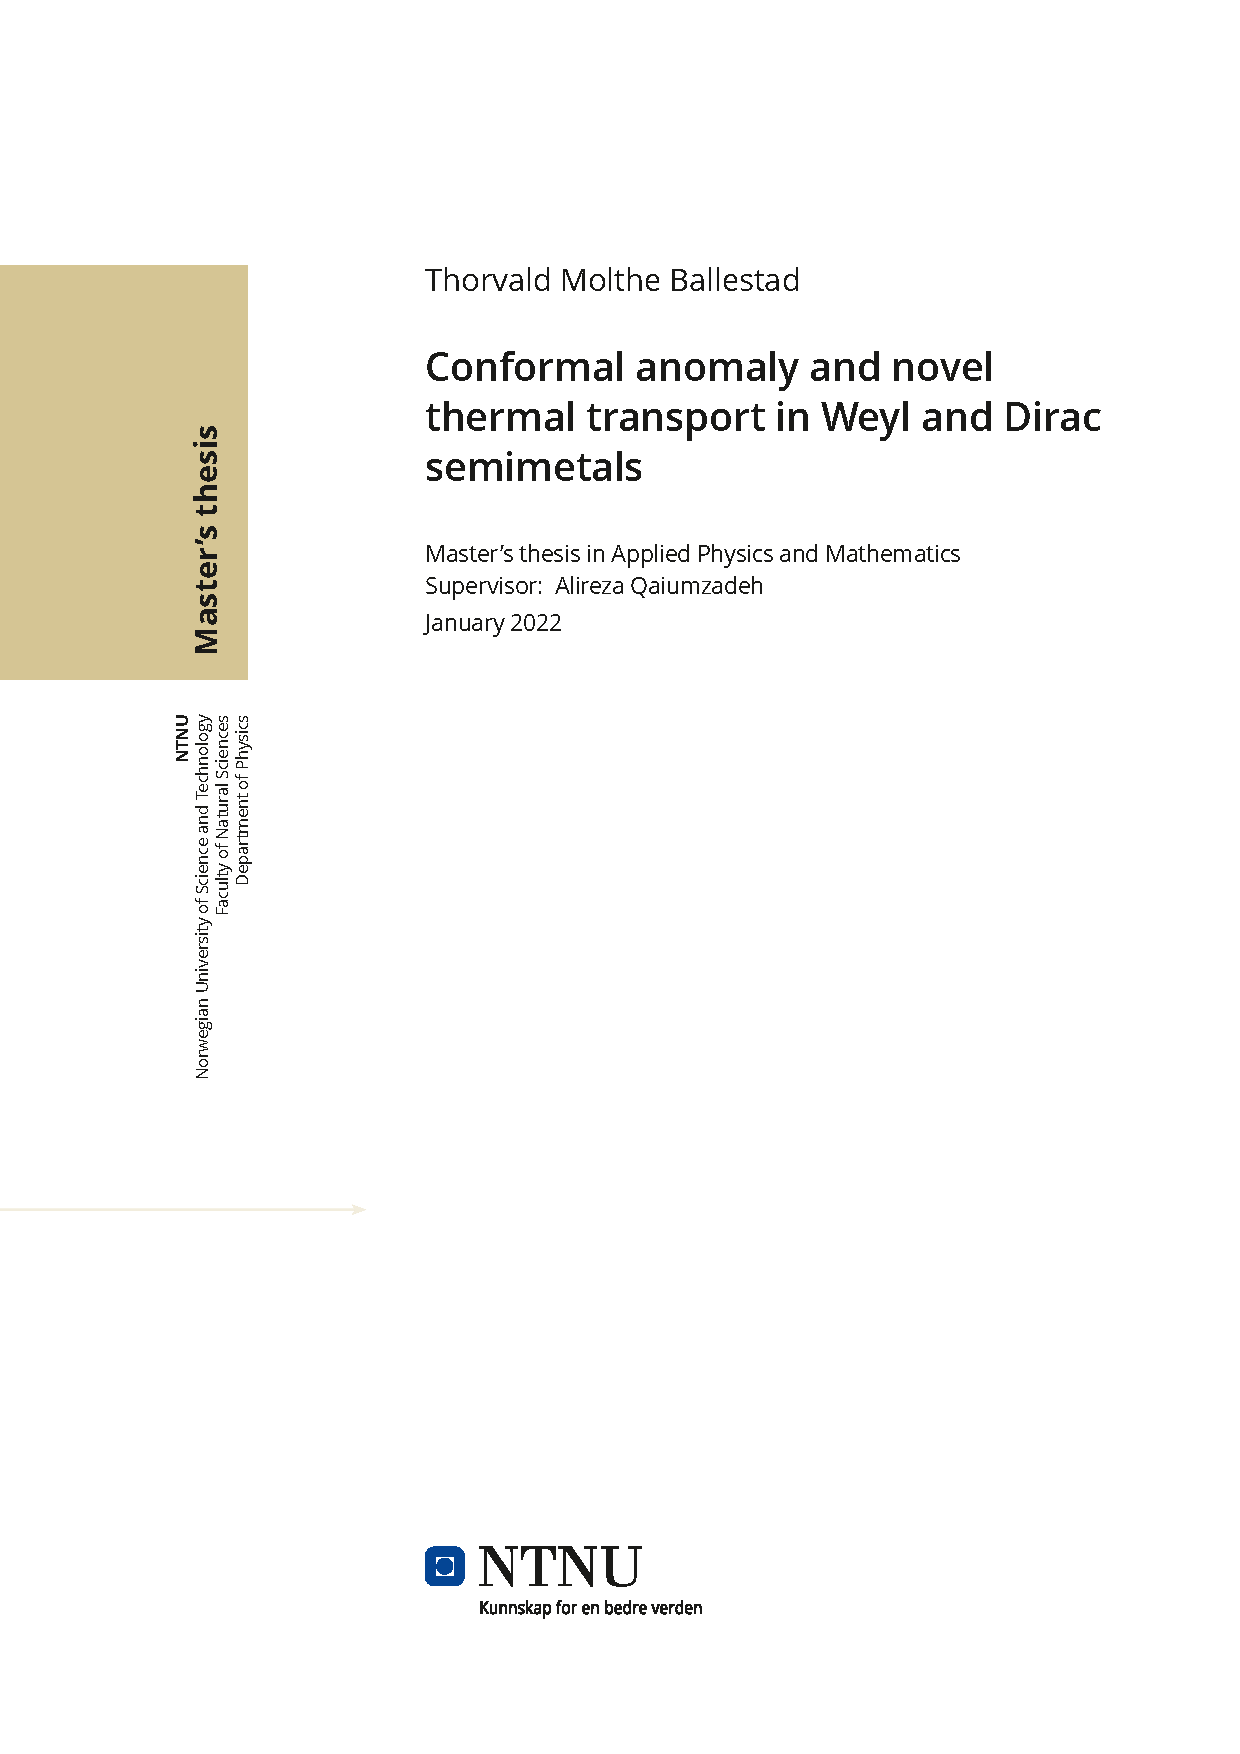
\includepdf[pages=-]{frontpagethesis.pdf}
\KOMAoptions{open=any}
\addchap{Preface}
This thesis constitutes the final part of a ``Sivilingeniør'' (M.Sc.) degree in Physics and Mathematics at the Norwegian University of Science and Technology.
It was written during the spring of 2022, after a five-year study program.
All notes, Mathematica programs, figures, and other files may be found at \href{https://github.com/Northo/MasterThesis}{\textsf{GiHub: https://github.com/Northo/MasterThesis}}.%
\footnote{Which will be made public \emph{after} grading of the thesis, due to plagiarism concerns.}

I would like to thank my supervisor, Alireza Qaiumzadeh, for excellent guidance throughout this last year.
This has been a novel topic for both of us, and our weekly meetings have been filled with interesting discussions and conversations.
% Thank you for guiding me through enormous amounts of information, and helping me see what was relevant.
Thank you for being a guiding lantern through an overwhelming maze of information, letting me see what is relevant and what is not.

Furthermore, I want to thank
\href{https://wp.icmm.csic.es/field-theories-in-condensed-matter-physics/vozmediano/}{María A. H. Vozmediano}\footnote{Materials Science Factory, Instituto de Ciencia de Materiales de Madrid, CSIC, Cantoblanco, 28049 Madrid, Spain\label{address-of-spain}.}
and
\href{https://wp.icmm.csic.es/field-theories-in-condensed-matter-physics/alberto-cortijo/}{Alberto Cortijo}\footnotemark[1]
for excellent discussions during the finalization of the thesis.
Through our meetings, the significance and interpretation of the results were made more clear, and interesting questions and continuations discussed.
It was also reassuring to hear that you had struggled with some of the same issues that we have faced.

The work presented in this thesis is currently being worked into a manuscript written primarily by me and Alireza, in collaboration with Maria and Alberto.


{
  \vfill
  \centering
  \color{black!80}
  \hrulefill\bigskip\\
  \parbox{0.84\textwidth}{
    \centering
    \texttt{This document has been typeset with the intention of printing on B5 paper. Consequently, the text and figures will look too large when printed on A4 paper.}
  }\\
  \bigskip\smallskip\hrulefill
  \vfill
}

\addchap[Summary | Oppsumering]{Summary}
Emergent Dirac equations in topological condensed matter physics may, as opposed to their high energy physics equivalents, have Lorentz-breaking terms.
Several such systems have been discovered both theoretically and experimentally, among them the tilted Dirac and Weyl semimetals.
Non-tilted Dirac and Weyl semimetals have previously been shown to house a transverse thermoelectric effect, a Nernst contribution.
The origin of the effect is the conformal anomaly, a quantum anomaly related to non-flat spacetime.
The effect, importantly, is finite even for zero chemical potential and temperature.
Using the Kubo formalism, we have extended the calculation to find the response function for a system with tilt.

Using Luttinger's relation, we introduce an effective gravitational field from a thermal gradient, which couples to the energy density.
By employing the conservation of energy, we then reformulate the response as a response to the derivatives of off-diagonal elements of the energy-momentum tensor.

We find the effect to be tunable by the direction and magnitude of the tilt with respect to the magnetic field.
Several possible candidates for experimental signatures are presented.
% and this may thus give a possible venue for further experimental investigation of the effect.
This work thus enables further experimental and theoretical investigation into the effect.
Furthermore, we show the importance of the specific choice of the energy-momentum tensor, which for non-zero tilt directly affects the computed response.
The ambiguity of the energy-momentum tensor is well known, however, our results show explicitly that in these types of systems, the choice is not only a conceptual formality but has qualitative consequences.


\addchap{Summary}
Non-tilted Dirac and Weyl semimetals have previously been shown to house a transverse thermoelectric effect, a Nernst contribution.
The origin of the effect is the conformal anomaly, a quantum anomaly related to non-flat spacetime.
The effect, importantly, is finite even for zero chemical potential and temperature.
Using the Kubo formalism, we have extended the calculation to find the response function of tilted Dirac and Weyl semimetals.

Using Luttinger's relation, we introduce an effective gravitational field from a thermal gradient, which couples to the energy density.
By employing the conservation of energy, we then reformulate the response as a response to the derivatives of off-diagonal elements of the energy-momentum tensor.

We find the effect to be tunable by the direction and magnitude of the tilt with respect to the magnetic field.
% Several possible candidates for experimental signatures are presented, and this may thus give a possible venue for further experimental investigation of the effect.
Several possible candidates for experimental signatures are presented.
This work thus enables further experimental and theoretical investigation into the effect.
Furthermore, we show the importance of the specific choice of the energy-momentum tensor, which for non-zero tilt directly affects the computed response.
The ambiguity of the energy-momentum tensor is well known, however, our results show explicitly that in these types of systems, the choice is not only a conceptual formality but has qualitative consequences.

% LTeX: language=no-NO
\addchap*{Oppsummering}
Effektive Dirac likninger i topologisk faststoff-fysikk kan, i motsetning til høy-energi ekvivalentene, ha ledd som bryter Lorentz invarianse.
Flere slike systemer har blitt oppdaget, både teoretisk og eksperimentelt, deriblant skråstilte Dirac og Weyl semimetaller.
% Det har tidligere blitt vist at ikke-skråstilte Dirac og Weyl semimetaller gir opphave til transversale ladningsstrømmer som respons på temperaturgradienter i magnetiske felt, en Nernst effekt.
Det har tidligere blitt vist at ikke-skråstilte Dirac og Weyl semimetaller gir opphave til en transversal  termoelektrisk effekt, et bidrag til Nernst effekten.
Effektens opphav er den konforme anomaliteten, en kvante-anomalitet relatert kurvet romtid.
Effekten består, viktig nok, også ved null kjemisk potensiale og temperatur.
Vi har generalisert utregningen til skråstilte systemer, ved hjelp av Kubo-formalismen.

Gjennom Luttingers relasjon introduserer vi et effektivt gravitasjonsfelt fra en termiske gradient, som vekselvirker med energitettheten.
Ved bevaringsloven for energi, kan dette omformuleres som en respons på den deriverte til ikke-diagonale elementer av energi-impuls-tensoren.

Vi ser at effekten er justerbar ved retning og størrelse på skråstillingen i forhold til magnetfeltet.
Flere kandidater til eksperimentell signatur presenteres, og dette kan dermed være en mulighet for videre eksperimentell utforsking av effekten.
Videre viser vi viktigheten av valg av energi-impuls-tensoren, som for skråstilte systemer påvirker resultatet av beregningen.
Tvetydigheten rundt definisjonen av tensoren er vellkjent, men vårt resultat viser eksplisit at i denne typen systemer, så har valget ikke bare konseptuell betydning, men direkte kvalitative effekt.
% LTeX: language=en-US
  % English and norwegian
\KOMAoptions{open=right}  % summary and oppsumering on same sheet
\addchap{Conventions and Symbols}
\begin{itemize}
\item $e$ is the fundamental charge, i.e. $e = |e|$.
\item $l_B$ is the characteristic length of a $B$-field, given as $l_B= \sqrt{\hbar /eB}$, with $e$ the fundamental charge defined above.
\item The signature of the Minkowski metric is taken to be $-2$, i.e. the metric tensor $\eta _{\mu \nu } = \operatorname{diag} (+1, -1,-1,-1)$.
\item The Fourier transform will be taken to be on the asymmetric form, with opposite sign of the temporal and spatial part, thus treating it as a four vector.
  For a $3+1$ dimensional case ($\vec{q}$ three dimensional), the Fourier transform is defined as
  \begin{equation}
    \label{eq:define-fourier}
    A(\vec{q}, \omega )\! =\!\!
    \iint \mathrm{d}t \mathrm{d} \vec{r}
    e^{i(\omega  t - \vec{q} \vec{r} )}
    A(\vec{r}, t),
    \;
    A(\vec{r}, t) =\!\!
    \iint 
    \frac{\mathrm{d}\omega  \mathrm{d} \vec{q}}{(2\pi )^4}
    e^{-i(\omega  t - \vec{q} \vec{r} )}
    A(\vec{q}, \omega).
  \end{equation}
  For other dimensionalities, the exponent of the $2\pi $ factor must be chosen accordingly.

\item Vectors will be written in bold font, $\vec{v} = (v_1, v_2, v_3)$, and with Roman indices, $i, j, k$, for two and three-dimensional vectors.
  Four dimensional vectors will be typed in normal weight, $v$, with Greek indices, $\mu ,  \nu , \lambda $, and upper and lower indices indicating contravariant and covariant quantities
\item Natural units \( \hbar = c = 1 \) will be used in parts of the thesis, for more clear notation and in order to make it easier for the reader to recognize the similarities with high energy physics literature.
\item For spin degrees of freedom, the Pauli matrices
  % \begin{equation}
  %   \sigma _1 =
  %   \begin{pmatrix}
  %     0 & 1\\ 1 & 0
  %   \end{pmatrix},
  %   \quad
  %   %
  %   \sigma _2 =
  %   \begin{pmatrix}
  %     0 & -i\\ i & 0
  %   \end{pmatrix},
  %   \quad
  %   %
  %   \sigma _3 =
  %   \begin{pmatrix}
  %     1 & 0\\ 0 & -1
  %   \end{pmatrix},
  % \end{equation}
  will be denoted by $\sigma $ for real spin and $\tau $ for pseudo-spin.
  
\item Operators will in general be typed with as normal quantities: $O$ for scalar operators and $\vec{O}$ or $O$ for vector operators, depending on their dimensions.
  The hat symbol, $\hat{O}$, will not be used unless not including a hat will be confusing.

\item In Chapter \ref{ch:charge-current}, we will use capital letters \( M, N \) to indicate the absolute value of the corresponding quantity, \( M = |m| \).
\end{itemize}


\tableofcontents

\mainmatter
\addchap{Introduction}
% What has been done
% What will we do
% Why is it nice?
%
% Topological materials
% Analogous to high energy
% Chiral and gravitational-chiral anomaly
% Conformal anomaly
Topological materials have been of central interest in contemporary condensed matter physics~\cite{fruchartIntroductionTopologicalInsulators2013}, with the first topological phases arising in the context of integer quantum Hall effect~\cites{klitzingNewMethodHighAccuracy1980}[as cited in][]{fruchartIntroductionTopologicalInsulators2013}.
A solid understanding of the topological theory behind this has been developed during the last decade and a half~\cite{fruchartIntroductionTopologicalInsulators2013, bernevigTopologicalInsulatorsTopological2013}, with the Nobel Prize in Physics 2016 awarded for theoretical work on topological matter~\cite{royalswedishacademyofsciencesNobelPrizePhysics}.
An excellent review of topological materials is given in~\cite{fruchartIntroductionTopologicalInsulators2013}.

One interesting phenomenon in topological materials is the emergence of quantum anomalies and the emergent particles' analogy to fundamental particles in \gls{qft}.
% One interesting phenomenon in topological materials is the emergence of quantum anomalies; the emergent particles follow in wonderful mathematical analogy to fundamental particles of quantum field theory.
% One interesting phenomenon in topological materials is the emergence of effective particles with strong analogy to the fundamental particles of \gls{qft}, even housing quantum anomaly effects.
Noether's theorem says that for any continuous symmetry of the action of a system, there is an accompanying conserved current.
This explains, for example, the conservation of momentum and energy as a result of the position and time independence of our universe.
In a quantum mechanical treatment, however, the symmetry of the classical theory may be broken, which gives rise to an \emph{anomaly}.
The chiral anomaly, for example, has been of great interest in condensed matter research in recent years~\cite{arjonaFingerprintsConformalAnomaly2019}.
The chiral anomaly explains the non-conservation of the axial current~\cite{zeeQuantumFieldTheory2010}, and gives rise to exotic transport phenomena in condensed matter systems~\cite{burkovChiralAnomalyTransport2015, wehlingDiracMaterials2014, burkovTopologicalSemimetals2016}.
A less investigated anomaly is the conformal anomaly, the appearance of a non-vanishing trace of the energy-momentum tensor in a conformally scaled metric.
Transport from the conformal anomaly has recently been investigated and shown in Weyl and Dirac semimetals~\cite{chernodubAnomalousTransportDue2016, chernodubGenerationNernstCurrent2018, arjonaFingerprintsConformalAnomaly2019}.

In this thesis, we extend the Kubo calculation done by~\textcite{arjonaFingerprintsConformalAnomaly2019} to find charge current response to thermal perturbations in \emph{tilted} Dirac and Weyl semimetals -- Lorentz breaking extensions of the Dirac equation.
The work combines important theory and concepts from both high energy and condensed matter physics.

The thesis consists of four chapters;
the three first chapters introduce concepts central to the main derivation of the thesis, while the fourth chapter represents the bulk work of the thesis, namely the derivation of the transverse charge current response from thermal perturbations in tilted Dirac and Weyl semimetals.
Note that some sections of the first and second chapter, and most of the third chapter, started as parts of a specialization project report written in the fall of 2021.

The first chapter gives an overview of concepts important to topological materials, starting with symmetries and ending with a more in-depth discussion of Weyl and Dirac semimetals, with a special focus on the tilted type.
In the second chapter, linear responses theory is introduced in light of the Kubo formalism and the Luttinger formalism of thermal transport.
In chapter three, we introduce anomalies of \gls{qft} in the context of high-energy physics.
The thesis also contains three appendices;
\cref{cha:long_expression} contains long expressions not included in the main text, \cref{sec:otherterm-appendix} contains a lengthy calculation that runs somewhat in parallel to the main text, for an alternative choice of the energy-momentum tensor (details discussed in the main text), and lastly, \cref{sec:aux-appendix} contains several minor results the author finds interesting, that are only tangentially relevant to the main work.


% The thesis consists of four chapters;
% the first three chapters introduce central concepts to the derivation, namely topological materials, with a focus on Weyl and Dirac semimetals; linear response theory; and anomalies in quantum field theory.
% The fourth chapter is the derivation of the response function, combining all the previous concepts.
% Note that some sections of the first and second chapter, and most of the third chapter, were initially written for a specialization project report.

% \part{Background material}

\chapter{Topological Materials}
In this chapter, we consider various concepts from physics that are relevant in the context of topological materials.
Firstly, the symmetry-related concepts of parity, time-reversal, Kramer's degeneracy, and accidental degeneracy are explained.
Then follows a quick summary of spin-orbit interactions.
Lastly, Weyl and Dirac cones are discussed, with particular focus on \emph{tilted} cones.
The chapter is intended as a quick introduction to the vast field of topological materials for someone who is not familiar with these concepts.

Some topics discussed are directly applicable to the thesis, while others are included both in order to put the concepts of the thesis in a greater context, and also with regard to further continuation of this work.
\section{Parity}
%% Much of this is taken from
%% Sakurai
We consider now the discrete transformation of space inversion, or \emph{parity}.
Firstly, basic properties of the transformation will be presented and discussed.
Its effect on the position, momentum, and angular momentum operators will be discussed, before a more general discussion on how it transforms proper- and pseudo-tensors.
% This will be applied to see how the parity transformation affects electric and magnetic fields.

Let the parity operator $P$ be a unitary operator
\begin{equation}
  P: \quad \ket{a} \rightarrow P\ket{a}.
\end{equation}
By definition, we require
\begin{align}
  P^\dagger x P &= -x,\\
  P^\dagger p P &= -p,
\end{align}
where $x, p$ are the position and momentum operators.
By the unitarity of $P$, which means that $P^\dagger P = I$,
$$
xP = -Px.
$$
We now use this anticommutation to find an explicit form of the transformation in the position representation.
By noting that, given the position eigenstate $\ket{x_1}$,
\begin{equation}
  x P\ket{x_1} = -P x_1\ket{x_1} = -x_1 P\ket{x_1},
\end{equation}
with $x_1$ the eigenvalue of the state, we may conclude
$$
P\ket{x_1} = \ket{-x_1}
$$
up to some arbitrary phase.
We chose this phase to be unity.
Then
\begin{equation}
  P^2 \ket{x_1} = \ket{x_1}
\end{equation}
for any position eigenstate, which  gives the  operator relation $P^2 = 1 \implies P = \pm 1$.
This also means that $P$ is Hermitian,
$$
P = P^{-1} = P^\dagger.
$$

The treatment of angular momentum is somewhat more involved.
Some sources simply state that as the orbital angular momentum
$$
L = x \times p
$$
is a product of two odd quantities, it must be even under parity.
This, of course, is a gross over simplification, as extra care must be taken when considering the spin angular momentum $S$ contributing to the total angular momentum
$$
J = L + S.
$$
The angular momentum operator is the generator of rotations
$$
R = e^{-i \epsilon J\cdot n} \approx 1 - i \epsilon J \cdot n
$$
where we expanded the operator under the assumption of a small angle, $\epsilon \ll 1$.
As rotations are invariant during space inversion,
\begin{align}
  P^\dagger R P &= R\\
 \mathllap{\implies\;} P^\dagger J \cdot n P &= J\cdot n
\end{align}
from which it follows that
\begin{equation}
P^\dagger J P = J,
\end{equation}
as the parity operator obviously does not act on the normal vector $n$.
Thus, the angular momentum operator, unlike the linear momentum operator, is even under parity.

For a general vector-like\footnote{We use the term \emph{vector-like} instead of vector, as the term vector is defined as something that is odd under parity, as opposed to for example a pseudo vector, even though they naively ``look'' like vectors. This can be compared to tensors. The definition of a tensor is something that transforms like a tensor under a Lorentz transformation, so we may have matrix objects that ``look'' like tensors, but transforms differently.} quantity $V$, we will consider how it transforms during space inversion.
If the quantity ``flips'' during space inversion, $P^\dagger V P = -V$, we say simply that it is a vector, also sometimes known as a polar vector.
Quantities that do not ``flip'', so that they turn into their opposites in the flipped image, we denote pseudo vectors.
Thus, depending on whether the eigenvalue of an operator under space inversion is $+1$ or $-1$ we say that it is either a pseudo-vector or vector, respectively.
Position and momentum are examples of vectors, while angular momentum and the magnetic field are examples of pseudo-vectors.
An illustrative explanation of this is shown in \cref{fig:pseudovector}, which explains both angular momentum and magnetic fields.

\emph{Remark about dimensionality}: The above discussion about parity, which is the standard way to present parity in condensed matter physics, is valid for three dimensions.
In two dimensions, however, one must separate \emph{parity} and \emph{space inversion}.
The former takes a right-handed system to a left-handed system~\cite{sakuraiModernQuantumMechanics2017}, while the latter inverts space, $\vec{x} \to  -\vec{x}$.
In odd dimensions this is the same, while in even dimensions they differ.
In even dimensions, inversion corresponds to a rotation, while a parity transform is different from any rotation.
In more formal terms, inversion is part of the group of proper  rotations $SO(n)$ for even dimensions, as the determinant is $+1$, the definition of a proper rotation.
Parity should in general be taken to be the operation $P$ such that the group of all rotations $O(n) = SO(n) \times \{E, P\}$, with $E$ the identity transformation.
This will not be of direct importance here, but it is an important detail to note.

\begin{figure}[h]
  \centering
  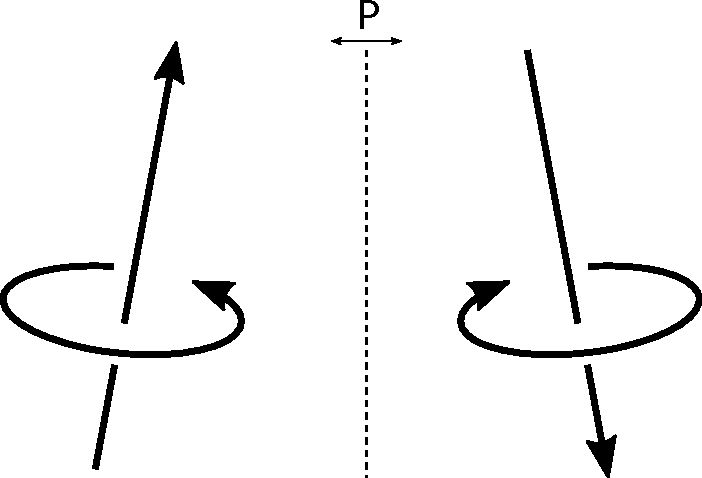
\includegraphics[width=0.5\textwidth]{figures/pseudovector}
  \caption{Schematic illustration of vectors and pseudovectors.
    A vector field with curl, which may be taken to be either momentum or current, is shown as a rotating arrow.
    The curl of this field, which will respectively be the angular  momentum or $B$-field, is shown as a straight arrow.
    Under inversion, shown as a mirror operation, the curl generated by the field is inverted in addition to the mirroring, i.e. rotated.
    This non-formal illustration gives an intuitive explanation of the concepts vector and pseudovector.
    Note that as the example is two-dimensional, mirror symmetry here the same as parity, and not inversion.
    See main text for details.
  }
  \label{fig:pseudovector}
\end{figure}

\section{Time reversal}
%% Much of this is taken from
%% Verneveig's Topological insulator ....
We will now consider the time reversal operator $\Theta $.
Firstly we will show that it must be antiunitary, then we will show $\Theta^2 = \pm 1$, and find a more specific form of $\Theta$ for half-integer spin systems.


The time reversal operator by definition will invert the value of the time
$$
\Theta: t \rightarrow -t
$$
while leaving space unchanged.
The invariance of space is summaries by the operator relation,
\begin{equation}
  \label{eq:TRdef}
  \Theta x \Theta^{-1} = x,
\end{equation}
where $x$ is understood as the position operator.
The momentum operator, however, is flipped due to its time dependence
\begin{equation}
  \label{eq:Pdef}
  \Theta p \Theta^{-1} = - p.
\end{equation}
A schematic representation of inversion symmetry and time reversal symmetry is given in Figure \ref{fig:symmetry_considerations}.

\begin{figure}[h]
  \centering
  \ref{leg_pos}
  \begin{tikzpicture}
    [
    every axis/.style={
      ytick=\empty,
      xtick={-3.14159, 3.14159},
      xticklabels={$-\pi$, $\pi$},
      every tick/.style={draw=none},
      xshift=0.2cm,
      anchor=left of south west,
      width=0.38\textwidth,
      xmin=-3.15, xmax=3.15,
      samples=201,
      cycle list name=linestyles,
      % legend to name=leg_pos,
      axis x line=bottom,
      xlabel=$k$,
    },
    every axis plot/.style={
      mark=none,
    }
    ]
    \begin{axis}[
      name=both,
      legend columns=2,
      axis y line=left,
      axis y line shift=10pt,
      ylabel=$E$,
      legend to name=leg_pos,
      ]
      \addplot {-cos(deg(x))}
      node[left]{$\uparrow$};
      
      \addplot {-cos(deg(x))}
      node[left]{$\downarrow$};
      \legend{$\uparrow$, $\downarrow$}

      \draw[<->] (-1, -0.540302306) node[below left]{$\downarrow, \uparrow$} -- (1, -0.540302306) node[below right]{$\downarrow, \uparrow$};
      \draw[very thin, gray, dotted] (0, -10) -- (0, 40);
    \end{axis}
    \begin{axis}[
      name=inversion,
      at=(both.right of south east),
      axis y line=none,
      ]
      \addplot {-cos(deg(x-1))}
      node[left]{$\uparrow$};
      
      \addplot {-cos(deg(x+1))}
      node[left]{$\downarrow$};
      
      \draw[<->] (-2.2, -0.362357754) node[above]{$\downarrow$} -- (2.2, -0.362357754) node[above] {$\uparrow$};
      \draw[very thin, gray, dotted] (0, -10) -- (0, 40);
    \end{axis}
    % \end{tikzpicture}
    % \begin{tikzpicture}
    \begin{axis}[
      name=time,
      at=(inversion.right of south east), 
      axis y line=none,
      ]
      \addplot {-cos(deg(x))}
      node[left]{$\uparrow$};
      
      \addplot {-cos(deg(x))+0.3}
      node[left]{$\downarrow$};
      
      \draw[<->] (-1, -0.24) node[above]{$\downarrow$} -- (1, -0.24) node[above]{$\downarrow$};
      \draw[very thin, gray, dotted] (0, -10) -- (0, 40);
    \end{axis}
    % \end{tikzpicture}
    % \begin{tikzpicture}
  \end{tikzpicture}
  \caption{Schematic illustration of time and inversion breaking of degenerate energy bands of a two-level system.
    The  two levels are denoted $\uparrow$ and $\downarrow$.
    \textbf{(Left:)} Both time-reversal and inversion symmetry present, with the two energy bands being degenerate at all momenta.
    \textbf{(Center:)} Inversion symmetry is broken. Notice how at the \gls{trim} points, $-\pi, 0, \pi$, the two energy levels are degenerate, as, by definition, we have $\vec{k} = -\vec{k}$.
    \textbf{(Right:)} Time reversal symmetry is broken.
    Notice how in the time reversal symmetric case Kramer's doublet is present, as for any state at $k$, the state at $-k$ is degenerate  in energy and has opposite spin.
    This is not the case when time reversal symmetry is broken, as the spin at  $-k$ has the same spin.
    Figure inspired by \citeauthor{ramazashviliZeemanSpinorbitCoupling2019}~\cite{ramazashviliZeemanSpinorbitCoupling2019}.
  }
  \label{fig:symmetry_considerations}
\end{figure}

We are now in a position to show that $\Theta$ must be antiunitary by requiring the invariance of the commutation relation between momentum and position, $[x, p] = i\hbar$.
\begin{equation}
  \Theta [x, p] \Theta^{-1} = \Theta i\hbar \Theta^{-1} = - [x, p] = -i\hbar.
\end{equation}
In the first equality, the commutation relation was used directly.
In the second equality, Eqs. (\ref{eq:TRdef}) and (\ref{eq:Pdef}) were used to gain a minus sign.
This all leads to the relation
\begin{equation}
  \Theta i \Theta^{-1} = -i.
\end{equation}
From this, we gather that the time reversal operator must be antiunitary.
An antiunitary transformation is a transformation
$$
\ket{a} \rightarrow \ket{\tilde{a}} = \theta \ket{a}, \quad 
\ket{b} \rightarrow \ket{\tilde{b}} = \theta \ket{b},
$$
such that
\begin{align}
  \braket{\tilde{b} | \tilde{a}} &= \braket{b | a}^*,\\
  \theta\left(c_1 \ket{a} + c_2 \ket{b}\right) &= c_1^* \theta\ket{a} + c_2^* \theta\ket{b}.
\end{align}
\emph{A note of caution:} the Dirac bra-ket notation was originally designed to handle linear operators, where it excels.
For anti-linear operators, which antiunitary operators are, the bra-ket notation can be deceiving.
We will always take anti-linear operators to work on kets, never on bras from the right.
So, for example,
$$ \braket{a| O | b} $$
should be understood as
$$ \bra{a} \left(\ket{O |b}\right)$$
and \emph{never}
$$ \left(\bra{a|O}\right) \ket{b}.$$
The left operation of an anti-linear operator on a bra, $\bra{a} O$, will not be defined.

We will in general write
\begin{equation}
  \label{eq:time-rev-def}
  \Theta = U K
\end{equation}
where $U$ is a unitary transformation and $K$ is the complex conjugation.
Now, we will show that $\Theta^2 = \pm 1$, by an elegant method inspired by~\citeauthor{bernevigTopologicalInsulatorsTopological2013}~\cite{bernevigTopologicalInsulatorsTopological2013}.
Consider
\begin{equation}
  \label{eq:1}
  \Theta^2 = UKUK = UU^* = U(U^T)^{-1} \equiv \phi,
\end{equation}
where we in the second last equality used the unitarity of $U$.
As applying the time reversal operator twice must result in the original state, up to some phase, $\phi$ must surely be diagonal.
From Eq. (\ref{eq:1}) it follows
\begin{equation}
  U = \phi U^T, \quad U^T = U \phi
\end{equation}
where the fact that $\phi^T = \phi$ for any diagonal matrix was used.
From this follows that
\begin{equation}
  U = \phi U \phi \Rightarrow U \phi^{-1} = \phi U.
\end{equation}
This holds in general only for $\phi = \pm 1$, and thus $\Theta^2 = \pm 1$.
Furthermore, we will later show that for integer spin particles $\Theta^2 = 1$ while for half-integer spin particles $\Theta^2 = -1$.

\subsection{Time reversal operator on spinful particles}
When considering spinful particles, we must enforce yet another property on the time reversal operator.
As spin is odd under time reversal one must have
\begin{equation}
  \label{eq:2}
  \Theta S \Theta^{-1} = -S.
\end{equation}
Consider now specifically a spin-$s$ state, with the basis $\ket{s, m}$, being an eigenstate of $S_z, \vec{S}^2$, with eigenvalues $m\hbar, s(s+1) \hbar^2$ respectively.
By Eq. (\ref{eq:2}) it follows that $\Theta \ket{s, m}$ is also an  eigenstate of $S_z$, with eigenvalue $-m \hbar $, since
\begin{equation}
  S_z \Theta \ket{s, m} = -\Theta  S_z \ket{s, m} = -m \hbar \Theta \ket{s, m}.
\end{equation}
Let
\[
  \Theta \ket{s, m} = \eta \ket{s, -m},
\]
where $\eta $ is some phase.
Consider now the commutation of the ladder operators $J_{\pm} = S_x \pm i S_y$ with the time reversal operator.
\begin{equation}
  \begin{split}
    \underbrace{\left[ S_x \pm i S_y \right]}_{S_{\pm}} \Theta  &= -\Theta S_x \mp i \Theta S_y\\
    &= -\Theta \underbrace{\left[ S_x \mp iS_y \right]}_{S_{\mp}},
  \end{split}
\end{equation}
where the anti-linearity of $\Theta $ is emphasized.
Thus, operating with $S_+$ on $\Theta \ket{s, m}$ gives
\begin{align}
  S_+ \Theta \ket{s, m} &= \eta_{sm} S_+ \ket{s, -m}\\
  &= \eta_{sm} \hbar \sqrt{(s+m) (s-m+1)} \ket{s, -m +  1}.
\end{align}
On the other hand, commuting the two operators first gives
\begin{align}
  S_+ \Theta  \ket{s, m} &= - \Theta  S_- \ket{s, m}\\
                         &= - \Theta \hbar \sqrt{(s+m)(s-m+1)} \ket{s, m-1}\\
  &= -\hbar \sqrt{(s+m)(s-m+1)} \eta_{s, m-1} \ket{s, -m + 1}.
\end{align}
By comparison, $\eta _{sm}= - \eta _{s, m-1}$; $\eta _{sm}$ has a flip of its sign under increments of $m$.
The $m$ dependence should therefore be $(-1)^m$.
For later convenience, we will choose to also include an $s$-term in the exponent, so that the exponent is integer also for half-integer systems, resulting in
\begin{equation}
  \eta _{sm} = (-1)^{s-m} f(s),
\end{equation}
where  $f(s)$  is some phase that does not depend on $m$.
We are now in a position where we may find $\Theta ^2$, by acting on a general spin $s$ system.
\begin{align}
  \Theta ^2 \sum\limits_{m = -s}^s a_m \ket{s, m} &= \Theta  \sum\limits_m^{} a^{*}_m f(s) (-1)^{s-m} \ket{s, -m}\\
                                                  &= \sum\limits_m^{} a_m f^{*}(s) (-1)^{s-m} \Theta \ket{s, -m}\\
  &= \sum\limits_m^{} a_m |f(s)|^2 (-1)^{2s} \ket{s, m}.
\end{align}
Note that it was important that $(-1)^{s-m}$ was real, which is taken care of by the $s$-term.
As $f(s)$ is only a phase, this gives
\begin{equation}
  \Theta ^2 = (-1)^{2s},
\end{equation}
for any spin $s$ system.
Thus, for half integer spin, $\frac{1}{2}, \frac{3}{2}, \dots $, $\Theta ^2 = -1$, while for integer spin $\Theta ^2= +1$.


\begin{comment}
  We implement this by letting the time reversal operator be a $\pi $ rotation of the spin, around some axis.
  Following the convention of considering this as a rotation around the $y$-axis, the $\Theta = UK$ operator gets the form~\cite{bernevigTopologicalInsulatorsTopological2013}
  $$
  \Theta = \eta e^{-i\pi S_y} K,
  $$
  where $\eta$ is some arbitrary phase and $S_y$ is the spin operator in the $y$-direction.
  Also, $\hbar = 1$ for ease of notation.
  Taylor expanding the exponential, splitting the terms into the $\sin$ and $\cos$ terms, and noting that
  \todo{TODO write something more legit here.}
  $$
  S_y^2 = \frac{1}{2}
  $$
  we can simplify the expression for $\Theta$.
  \begin{equation}
    \Theta = - i \eta \left(2 S_y\right) K.
  \end{equation}
  Thus, one gets
  \begin{equation}
    \Theta^2 =
    4 i \eta^2 S_y K i  S_y K =
    4 i \eta^2 S_y (-i S_y^*) =
    4 i \eta^2 S_y S_y^* =
    -4 i \eta^2 S_y^2.
  \end{equation}
\end{comment}

\section{Kramer's degeneracy}\label{sec:kramers}

%% Some of the material is inspired from
%% Sakurai and Napolitano

Kramer's degeneracy states that for any half-integer system that is time-reversal symmetric, energy levels are at least two-fold degenerate.
The proof of this is simple, and uses the fact that for any half-integer spin system, $\mathcal{T}^2 = -1$.
A heuristic way to see this is the fact that spin is odd under time-reversal, and for half-integer systems there is no zero-spin state, so reversing the spin cannot result in the same state.
\begin{Proof}
  Assume
  $$ [H, \mathcal{T}] = 0 $$
  and that $\ket{n}$ is an eigenstate of the system
  $$ H \ket{n} = E_n \ket{n}.$$\\
  Then
  $$
  H \mathcal{T} \ket{n} = \mathcal{T} H \ket{n} = \mathcal{T} E_n \ket{n} = E_n \mathcal{T} \ket{n}
  $$
  and so $\mathcal{T} \ket{n}$ is also an eigenstate with the eigenvalue $E_n$.
  To assert that the eigenvalue is in fact degenerate, one must also show that the two states are not the same ray.
  That is $\mathcal{T} \ket{n} \neq e^{i \delta} \ket{n}$, where $\delta$ is some phase.
  Suppose that the above is \emph{not} true, $\mathcal{T} \ket{n} = e^{i \delta} \ket{n}$.
  Then,
  $$
  \mathcal{T}^2 \ket{n} = \mathcal{T} e^{i\delta} \ket{n} = e^{-i\delta} \mathcal{T} \ket{n} = + \ket{n}.
  $$
  However, as was stated above, $\mathcal{T}^2 = -1$ for all half-integer systems.
  The assumption must therefore be wrong, and the eigenvalue is degenerate.
\end{Proof}
The two states, $\ket{n}$ and $\mathcal{T} \ket{n}$, are often referred to as Kramer's doublet.
Note that the two states have opposite spin.

\subsection{Generalization to time and parity symmetry}
Consider now a time-reversal and parity symmetric system, $[H, P \mathcal{T}] = 0$.
This will, similar to the case for time-reversal, make the energy levels at least two-fold degenerate.
\begin{Proof}
  Assume
  $$
  [H,P \mathcal{T}] = 0
  $$
  and that $\ket{n}$ is an eigenstate of the system
  $$
  H\ket{n} = E_n\ket{n}.
  $$
  Then
  $$
  H P \mathcal{T}\ket{n} =
  P\mathcal{T} H \ket{n} =
  P \mathcal{T} E_n \ket{n} =
  E_n P\mathcal{T} \ket{n}.
  $$

  Assume now that $P\mathcal{T} \ket{n} = e^{i\delta} \ket{n}$, which we will prove to be false.
  That would lead to
  $$
  (P\mathcal{T})^2 \ket{n} = P\mathcal{T} e^{i\delta} \ket{n}
  = \ket{n}.
  $$
  However, as $[P, \mathcal{T}] = 0$, we have
  $$
  (P\mathcal{T})^2 =
  P\mathcal{T} P \mathcal{T}=
  P\mathcal{T}^2 P=
  -1
  $$
  as $P^2 = 1$.
  As above, the states are thus different, and the eigenvalue is degenerate.
\end{Proof}

\section{Accidental degeneracy}
\label{sec:accidental-degeneracy}
In general, for a two level system depending on some parameter the energy levels of the two levels will not cross, i.e. be degenerate, unless there are symmetries in the system forcing them to be degenerate, as is the case in for example Kramer's degeneracy.
However, even without any symmetries
\footnote{There will always, for a degenerate system, be some symmetry, although it might be a \emph{hidden} symmetry. We here mean no a priori apparent symmetry.}
there will be so-called \emph{accidental degeneracies} if the parameter space is sufficiently large.
Consider a general two-level Hamiltonian
\begin{equation}
  H = f_1 \sigma_x + f_2 \sigma_y + f_3 \sigma_z,
\end{equation}
which will have an energy splitting between the two levels
\begin{equation}
  \Delta E = 2 \sqrt{
    f_1^2 + f_2^2 + f_3^2
  }.
\end{equation}
In general, we may solve $\Delta E = 0$ by tuning the three parameters simultaneously, and thus there must be degenerate points -- accidental degeneracies.
Supposing that the parameters $f_i$ can be expressed as functions of the momentum components, $f_i =f_i(p_i)$, this will correspond to degenerate points in momentum space.

If there are in addition some symmetry constraints on the system, the space of degenerate points may increase.
Suppose, for example, the system is time-reversal symmetric.
Recalling the time-reversal operator defined in \cref{eq:time-rev-def}
$$
\Theta = UK,
$$
with $U$ being a unitary operator and $K$ the complex conjugate, the imaginary Pauli matrix $\sigma_y$ must be excluded.
Thus, the solution to the closing of the band gap has a free parameter, and the degenerate space has dimension one.

\section{Spin-orbit interaction}
Spin-orbit interactions are not used directly in this thesis.
It is, however, relevant to include some superficial introduction to the subject, both in order to conclude that spin-orbit interactions are not something one has to consider in later derivations of this thesis, and also that it might prove useful in future applications of the ideas and theory discussed in the thesis.

Spin-$1 /2$ particles are in general governed by the Dirac equation.
In the non-relativistic regime, as is the case in condensed matter physics, we may reduce the equation to the Pauli equation.
This equation contains as a relativistic correction the spin orbit coupling term~\cite{engelTheorySpinHall2007}
\begin{equation}
  \label{eq:pauli}
  H_{SO} = \lambda_{\text{vac}} \vec{\sigma} \cdot ( \vec{k} \times \nabla \tilde{V}),
\end{equation}
where $\lambda_{\text{vac}}$ is a constant with dimension length squared, $\vec{\sigma}$ are the Pauli matrices representing spin, and $\tilde{V}$ is the total potential in the system.
In preparation of the considerations to come, split up the potential in the periodic crystal potential $V_\text{cr}$ and the remaining potential $V$ from impurities
\begin{equation}
  \tilde{V} = V_{\text{cr}} + V.
\end{equation}
\todo{Should this be the Bloch basis}
Changing basis to a quasi-particle picture of free particles, thus eliminating $V_\text{cr}$ from the equation, one gets the effective Hamiltonian~\cite{engelTheorySpinHall2007}
\begin{align}
  \label{eq:Heff}
  H_\text{eff} &= \epsilon_k + V + H_\text{int} + H_\text{ext},\\
  H_\text{int} &= -\frac12 \vec{b}(\vec{k}) \cdot \vec{\sigma},\\
  H_\text{ext} &= \lambda \vec{\sigma} \cdot( \vec{k} \times \nabla V).
\end{align}
Here, the subscripts denote the effective Hamiltonian $H_{\text{eff}}$, consisting of an intrinsic part, $H_{\text{int}}$, and an extrinsic part, $H_{\text{ext}}$.
$\vec{b}(\vec{k})$ is the intrinsic spin-orbit field, the part of the crystal potential $V_{cr}$ that is not eliminated by our change of basis.
As the intrinsic spin-orbit interaction should be time reversal invariant, we can argue that $\vec{b}$ must be an odd function.
\begin{equation}
  \Theta H_\text{int} \Theta ^{-1} = H_\text{int}
  \implies 
  \vec{b}(\vec{k}) \cdot \vec{\sigma} = -\vec{b}(-\vec{k}) \cdot \vec{\sigma},
\end{equation}
where the well known effects of the time reversal operator was applied to the momentum and spin, as $\Theta \vec{k} \Theta ^{-1} = -\vec{k}$ and $\Theta \vec{\sigma} \Theta ^{-1} = -\vec{\sigma}$.
Obviously, this means that inversion symmetry must be broken for the intrinsic interaction term  to be finite.
This is easily seen as, with $P$ being the parity operator,
\begin{equation}
  P H_\text{int} P^{-1} = H_\text{int} \Rightarrow
  \vec{b}(-\vec{k}) = \vec{b}(\vec{k}),
\end{equation}
since spin is invariant under inversion.


The external contribution to the spin-orbit interaction is contained in $H_\text{ext}$, which does not require any particular symmetry to be present.
A Zeeman term, where time reversal is broken, would be represented in the external part of the Hamiltonian.


The spin-orbit field $\vec{b}(\vec{k})$ may take many forms depending on the specifics of the system at hand.
The Dresselhaus term
\begin{equation}
  H_D = \alpha p_x (p_y^2 - p_z^2) \sigma_x + \text{c.p.}
\end{equation}
where c.p. denotes terms of circular permutation of the indices,~\cite{manchonNewPerspectivesRashba2015} and the Rashba term~\cite{wuTwoDimensionalGiantTunable2020}
\begin{equation}\label{eq:rashba}
  H_R = \alpha (p_y \sigma_x - p_x \sigma_y),
\end{equation}
are arguably the most well-known models.
% In the following we will compare and discuss the symmetries of the Rashba Hamiltonain compared to a Zeeman Hamiltonian.

We immediately see that the Rashba Hamiltonina (\ref{eq:rashba}) does not break time reversal invariance, as both momentum and spin are odd under time reversal.
It is however odd under inversion.
This is of course exactly opposite of a Zeeman term, where we introduce an external magnetic field, thus breaking time reversal symmetry.

Consider a free electron model where we add a Rashba term
\begin{equation}
  H = \frac{p^2}{2m} + \alpha (p_y \sigma _x - p_x \sigma _y).
\end{equation}
The Hamiltonian commutes with the momentum operator, so we may replace the momentum operator with its eigenvalue $\hbar k$.
Solving for the eigenvalue is straight forward, and gives
\begin{equation}
  E_{\pm} = \frac{\hbar k^2}{2m} \pm \alpha k,
\end{equation}
where $k=|\vec{k}|$.
We expect the eigenvalues to be linear combinations of spin up and spin down states, and also that the coefficients depend on $k$, as the Rashba term has copuled spin and momentum.
Take
\begin{equation}
  \psi_{\pm} = \frac{e^{i \vec{k} \vec{r}}}{\sqrt{2}} \left( \ket{\uparrow} + b \ket{\downarrow} \right),
\end{equation}
where $b$ is some phase we must find.
By inserting into the time-independent Schrödinger equation, we find $b = \mp i (k_x + k_y ) /k$, which is obviously $b=\mp i \exp (i \theta )$, where $\theta $ is the angle of the momentum, $\vec{k} = (k \cos \theta , k \sin \theta)$.
Using the matrix representation $\ket{\uparrow} = (1,0)^T, \ket{\downarrow} = (0,1)^T$, the eigenvalues are given as
\begin{equation}
  \psi _{\pm} =
  \frac{e^{i \vec{k} \vec{r}}}{\sqrt{2}}
  \begin{pmatrix}
    1\\
    \mp i e^{i \theta }
  \end{pmatrix}.
\end{equation}
These states have interesting spin expectation values
\begin{equation}
  \braket{\psi_{\pm} | \vec{\sigma} | \psi _{\pm}}
  =
  \pm
  \left[  
    \sin\theta \hat{x} - \cos \theta \hat{y}
  \right].
\end{equation}
The spin is orthogonal to the momentum, making a circular pattern around the origin.
The direction of the rotation defines the chirality of the state.
The spin together with the energy solutions are shown in Figure \ref{fig:rashba}.


\begin{figure}[hp]
  \centering
  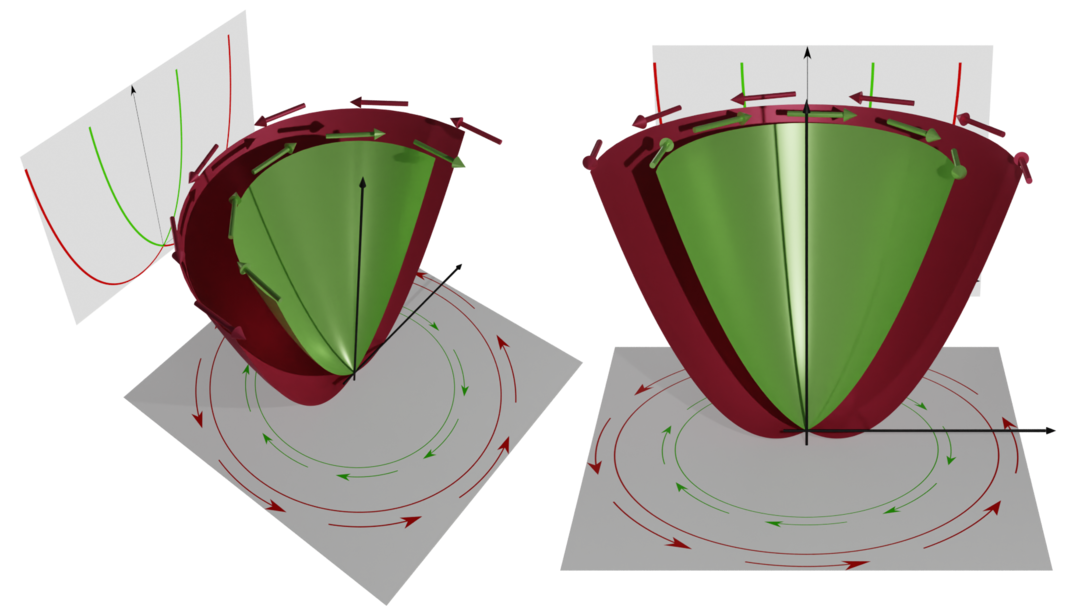
\includegraphics[width=\textwidth]{figures/rashba_combine-wside-small.png}
  \caption{Dispersion curves for a system with Rashba spin-orbit coupling. \textbf{Left:} Seen from above. \textbf{Right:} Seen from the front.
    The projection into the $xy$-plane is shown, as well as a cross section in a plane perpendicular to the $xy$-plane.
    The spin of the two states are shown as arrow above the dispersion curves, which defines the chirality of each state.
    Notice, as is most easily seen in the projection, that the two solutions together form a pair of parabolas separated in momentum.
  }
  \label{fig:rashba}
\end{figure}

% \begin{figure}[ht]
%   \centering
%   \begin{subfigure}[b]{0.48\textwidth}
%     \begin{tikzpicture}
%       \begin{axis} [
%         cycle list name=linestyles,
%         width=\textwidth,
%         ]
%         \addplot {(x-1)^2}
%         node[right]{$\uparrow$};
        
%         \addplot {(x+1)^2}
%         node[right]{$\downarrow$};

%         \draw[<->] (-3, 4) -- (3, 4);
%       \end{axis}
%     \end{tikzpicture}
%     \caption{Band splitting under SoC. Note that Kramer's doublet is not broken.}
%   \end{subfigure}
%   \begin{subfigure}[b]{0.48\textwidth}
%     \begin{tikzpicture}
%       \begin{axis} [
%         cycle list name=linestyles,
%         width=\textwidth,
%         ]
%         \addplot {(x)^2}
%         node[right] {$\uparrow$};
%         \addplot {(x)^2 + 10}
%         node[right] {$\downarrow$};

%         \draw (-3, 4) -- (3, 4);
%       \end{axis}
%     \end{tikzpicture}
%     \caption{Band splitting under Zeeman term. Note the breaking of Kramer's doublet.}
%   \end{subfigure}
%   \caption{Illustration of band splitting when lifting the degeneracy with Zeeman filed and SoC}
%   \label{fig:band_splitting}
% \end{figure}


\begin{comment}
\begin{figure}[ht]
  \centering
  \ref{named}  %% Legend
  \begin{tikzpicture}
    \begin{groupplot}[group style={
        group name=splitting,
        group size=2 by 1,
        horizontal sep=3pt,
      },
      xmin=-5, xmax=5,
      legend to name=named,
      cycle list name=linestyles,
      ]
      \nextgroupplot
      \addplot {(x-1)^2}
      node[left]{$\uparrow$};
      
      \addplot {(x+1)^2}
      node[left]{$\downarrow$};
      
      \draw[<->] (-3, 4) node[above]{$\downarrow$} -- (3, 4) node[above] {$\uparrow$};
      \draw[very thin, gray, dotted] (0, -10) -- (0, 40);

      \nextgroupplot[yticklabels={}]
      \addplot {(x)^2}
      node[left] {$\uparrow$};
      \addplot {(x)^2 + 10}
      node[left] {$\downarrow$};

      \draw[<->] (-3, 3^2) node[above]{$\uparrow$} -- (3, 3^2) node[above]{$\uparrow$};
      \draw[very thin, gray, dotted] (0, -10) -- (0, 40);

      \legend{$\uparrow$, $\downarrow$}
    \end{groupplot}
  \end{tikzpicture}
  \caption{Illustration of band splitting when lifting the degeneracy with Zeeman filed and SoC.
    For the SoC (left) Kramer's doublet is not broken. That is, there is an energy degeneracy with opposite spins and momentum.
    %\todo{find out if this is the actual definiton of Kramer's doublet}
    For the Zeeman case (right) Kramer's doublet is broken.}
  \label{fig:band_splitting}
\end{figure}
\end{comment}
\section[Weyl and Dirac cones]{Weyl and Dirac cones in condensed matter physics}
\label{sec:weyl-dirac-cones}
%% Much is taken from https://www.tandfonline.com/doi/pdf/10.1080/00018732.2014.927109?needAccess=true
Dirac and Weyl cones are the emergence of non-gapped linear energy bands in condensed matter physics, in effect exhibiting relativistic behavior at non-relativistic speeds.
We here give a brief introduction to these materials.
The system and its relation to high energy physics is discussed first.
Then, several perturbations of the system are introduced.
The topological nature of the system is considered in the context of Chern numbers and Berry curvature.
Lastly, we go into tilted Dirac cones in some more depth.
The reader is also advice to consult the many recent reviews on the topic, notably \textcite{armitageWeylDiracSemimetals2018} for a general introduction and overview of the field, \textcite{jiaWeylSemimetalsFermi2016} with a focus on material realizations, and \textcite{chernodubThermalTransportGeometry2021} which is the most directly relevant for our work, discussing in particular thermal transport and the analogy to high energy physics.

% Firstly, we will consider the so-called band crossing, and how the opening of a gap at the band crossing behaves differently in two and three dimensions.
% Then, various perturbations that do not open a gap will be considered, giving interesting effects in the dispersion relations.
% Lastly, a consideration of these materials in light of Berry curvature and the topological quantity of Chern numbers will be given.

The standard model for metals in condensed matter physics is the Landau Fermi liquid \cites{landauTheoryFermiLiquid1956,chernodubThermalTransportGeometry2021}, where electrons are described by the Hamiltonian \( p^2 /2 m^* \), with \( m^* \) some effective mass.
The model works remarkably well for many systems, but fails for Dirac materials, where the electrons behave as ``Dirac fermions''.
The notion of a ``Dirac fermion'' is almost comical from a high energy point of view\cites{chernodubThermalTransportGeometry2021,vozmedianoTheoreticalPhysicsColloquium2021} -- what else can they be?
A fermion is by its very definition a Dirac spinor.
In condensed matter language, however, we mean by fermion that it obeys the Pauli exclusion principle and follows the Fermi-Dirac distribution.
By Dirac fermion in condensed matter we mean fermions whose effective Hamiltonian is linear in momenta, they obey an effective Dirac equation.

This field unifies concepts from high and low energy physics;
a ``new era of grand unification of low and high energy phiscs'' as \textcite{chernodubThermalTransportGeometry2021} puts it.
The emergent Dirac and Weyl cones in condensed matter physics follow in beautiful analogy their high energy counterparts.
Thus, the theory and results from high energy physics may be applied in these emergent Dirac systems.
Likewise, these materials offer the opportunity to probe the fundamental theories of our universe, and beyond, at much lower energy and cost scales.
% Unfortunately, some concepts of \gls{qft} and high energy physics are somewhat inaccessible for condensed matter physicists.
Unfortunately, the language of \gls{qft} and high energy physics is somewhat inaccessible for condensed matter physicists.
At the same time, the condensed matter descriptions have been difficult to relate back to the \gls{qft} formalism.
So while the intersection of the two fields offer the possibility of great new insight, it also comes with some misunderstandings.
Some phenomena are known under different names, while different phenomena may be mistaken for the same.
The recent and excellent review paper by \textcite{chernodubThermalTransportGeometry2021} attempts to make the topics approachable for researchers from both fields, with its ``main purpose [...] to present the basic notions underlying new developments in condensed matter in a language equally accessible to both high energy and condensed matter communities''.

We wish here to briefly illuminate the connection between the high energy Dirac theory and the Dirac and Weyl semimetals of condensed matter physics, assuming the reader to be an expert in neither.
The (massive) Dirac equation reads
\begin{equation}
  (i \slashed{\partial} - m ) \psi = 0,
\end{equation}
where \( \slashed{\partial} = \gamma^{\mu} \partial_{\mu} \), \( \gamma^{\mu} \) are the so-called \emph{gamma matrices} \footnote{Also known as the Dirac matrices. They are any irreducible matrix representation of the Clifford algebra.}, \( m \) is some mass parameter, and \( \psi \) the Dirac spinor.
Note also that natural units \( c = \hbar = 1 \), as usual, is used and that the systems is \( 4\times 4 \).
It may of course be written as the Schrodinger equation\cite{chernodubThermalTransportGeometry2021} \( i \partial_t \psi = H \psi \), with \( H = \gamma^0 m + \gamma^0\gamma^ip_i \).
The great insight of Dirac, was that due to the requirement of Lorentz invariance, the momentum and time operators had to appear at the same order, as opposed to the standard free particle \( H = p^2 /2m \).
% The great insight of Dirac, was that the momentum and time operators had to appear at the same order, due to the requirement of Lorentz invariance.
Shortly after Dirac published his theory, Weyl commented that for a massless particle, the equation could be decomposed into two \( 2 \times 2 \) equations -- a Weyl decomposition.
This yields two independent subsystems, themselves also linear in momentum,
\begin{equation}
  \label{eq:156}
  H_{\pm} = \pm \vec{\sigma} \cdot \vec{p},
\end{equation}
with the \( \pm \) defining the \emph{chirality}.

Interestingly, massless Dirac fermions may appear in condensed matter as low energy effective descriptions of electronic systems near a two-band crossing.
Instead of obeying the Landau Fermi liquid theory, as most materials, they obey a Dirac equation, with the speed of light being replaced by the Fermi velocity $v_F$.
As in the high energy case, the Dirac equation may be decomposed into chiral Weyl equations
\begin{equation}
  \label{eq:3}
H_D = s v_{F} \vec{\sigma} \vec{p},
\end{equation}
where $\vec{\sigma}$ are the Pauli matricies, $v_F$ the Fermi velocity, $\vec{p}$ the momentum, and $s=\pm 1$ denotes the chirality.
% It is here important to note that the spin degree of freedom expressed by the Pauli matricies, may either be real spin or some pseudo spin degree of freedom.
It is here important to note that the Pauli matrices represent either real spin degree of freedom or some pseudo spin degree of freedom.
Examples of pseudo spin is that of bipartite lattices, such as Graphene, in which case one must be careful when for example applying time reversal, as only real spin is odd under this operation, and not pseudo spin.

These linear low energy emergent systems may appear in both 2D and 3D.
There are, however, important differences depending on the dimensionality.
When we here refer to Dirac and Weyl materials, we always mean 3D systems, which has become the norm in the literature.
In some older literature, the term might also be applied to 2D systems, such as graphene.

\label{sec:stability-of-gap}
The dispersion of the Hamiltonian (\ref{eq:3}) has a band crossing at  $\vec{p} = 0$.
For the two-dimensional case, a perturbation on the form $m \sigma_z$, with $m$ some parameter, opens a gap in the dispersion.
This is easily verified by writing out the Hamiltonian and solving the eigenproblem
\begin{align}
  H_D^{(2D)} &= s v_{F} (p_x \sigma_x + p_y \sigma_y) + m \sigma_z,\\
  \left|
  H_D^{(2D)} - E
  \right| &= 0.
\end{align}
As the Hamiltonian commutes with the momentum operator, we replace the momentum operator with its eigenvalues
\begin{equation}
E_{\pm} = \pm v_F \hbar \sqrt{k_x^2 + k_y^2 + \frac{m^2}{\hbar ^2 v_{F}^2}}.
\end{equation}
For a finite \( m \), there are no solutions $k_x, k_y$ making the energy levels degenerate (i.e. \( E_{\pm} = 0 \)).
The crossing is thus only protected by symmetry considerations, and is not \emph{topologically protected}.
\todo{Is this usage of topologically protected correct?}


In three dimensions the situation is somewhat different, with the Hamiltonian  
\begin{equation}
  H_D^{(3D)} = s v_F ( p_x \sigma_x + p_y \sigma_y + p_z \sigma_z).
\end{equation}
In this case, no perturbing term may open a gap at the crossing.
There is no $2\times 2$ matrix $\sigma_4$ that anticommutes with the Pauli matrices and while also being linearly independent, i.e. there is no ``fourth'' Pauli matrix;
therefore no perturbative term will open the gap.
Say for example we add a term like $m \sigma_z$, where the $z$-direction was chosen arbitrarily.
The only effect this will have on the crossing is to translate it in $p_z$.
Tying this back to the accidental degeneracy of section \ref{sec:accidental-degeneracy}, we see that no matter the perturbation, the three-dimensional momentum space will always have a point of degeneracy, i.e., a crossing.
The crossing is \emph{topologically protected}.
A more formal approach to topological materials, is that of topological invariants -- numbers related to the topology of the material.
Having a non-trivial topological invariant number, is the very definition of topological materials, and we will in subsection \ref{sec:chern-number-weyl} show that Dirac cones makes the Chern number of these materials non-trivial.

Opposed to high energy physics, the emergent Dirac equation in condensed matter physics need of course not be Lorentz invariant.
We may therefore introduce terms that break Lorentz invariance.
Introduce to the system a pseudospin degree of freedom, thus extending the system to $4\times 4$-matricies;
in effect re-construct the full Dirac equation from the Weyl equations, and then introduce perturbations.
The Hamiltonian of the system
\begin{equation}
  \label{eq:5}
  H = v_F \tau _x \otimes \vec{\sigma} \vec{p} + m \tau _z \otimes I_2 + b I_2 \otimes \sigma _z + b' \tau _z \otimes \sigma _x,
\end{equation}
with $\vec{\tau}$ the Pauli matrices related to the pseudospin, and $I_2$ the identity matrix of dimension 2.
The perturbing parameters $m, b, b'$ are a mass parameter, and Zeeman fields in the $z$ and $x$ direction, respectively~\cite{armitageWeylDiracSemimetals2018}.
Ignore for now $b'$, i.e. $b' = 0$, which is related to a state known as the line node semimetal.
Notice that the $b$ term breaks time reversal symmetry in the system, as the real spin $\sigma $ is odd under time reversal.
The eigenvalues of this system~\cite{armitageWeylDiracSemimetals2018}
\begin{equation}
  E_{s \mu }(\vec{k}) = s \left[
    m^2 + b^2 + v_{F}^2k^2 + 2 \mu  b \sqrt{v_F^2 k_z^2 + m^2}
  \right]^{\frac{1}{2}},
\end{equation}
with $s=\pm 1, \mu = \pm 1$ encoding the degeneracies related to the spin and pseudospin degrees of freedom, respectively.
There are still linear dispersions for $b > m$, for $b < m$, a gap opens, and the dispersion is non-linear.
In fact, for \( b > m \), the perturbation is simply a shift in $k_z$ of the Dirac cone, as  is seen by rewriting
\begin{equation}
  E_{s \mu }(\vec{k}) = s v_F
  \left[
    k_x^2 + k_y^2 + \left( \sqrt{k_z^2 +  \frac{m^2}{v_{F}^2}} + \mu \frac{b}{v_{F}} \right)^2
  \right]^{\frac{1}{2}}.
\end{equation}
This still has Weyl node solutions at $k_z^2 = (b^2-m^2) /v_F^2$, where the dispersion is linear in the vicinity of the nodal solutions.
This thus separates two Dirac nodes in momentum space, giving  a \emph{Weyl} semimetal.
This also illustrates that the decomposition in Eq. (\ref{eq:3}) is valid around either of the shifted nodes.
Expanding around one of the Dirac points of the Weyl semimetal, the Hamiltonian is exactly Eq. (\ref{eq:3}), after decomposing the $4 \times 4$ Hamiltonian into its two chiral  $2\times 2$ Weyl constituents.
If one instead perturbs the system with a Zeeman field in the $x$-direction, $b' \neq 0$, the separation is instead in energy, giving nodal loop where the two cones intersect.
We will not go into any depth on these types of materials.

The three cases described here: unperturbed, where the two cones are superimposed; perturbed by $b$, where the cones are separated in momentum; and perturbed by $b'$, where the cones are separated in energy, are shown in Figure~\ref{fig:conetypes}.
Notice that in the two latter cases, the Dirac points, i.e. crossings, are not superimposed.
As will be substantiated more in section \ref{sec:chern-number-weyl}, this makes the crossings very robust, as the two nodes must merge before a gap may be opened.


The Hamiltonian in Eq.~(\ref{eq:3}) is not the most general \( 2 \times 2 \) Weyl system, if we allow for anisotropy in the system.
In three dimensions we have more generally the \emph{tilted} Weyl Hamiltonian
\begin{equation}
  \label{eq:4}
  H_s = (\vec{t}^{s} + s \vec{\sigma}) (\vec{v} \odot \vec{p}),
\end{equation}
where $\vec{t}$ is  the \emph{tilt vector}, $\vec{v}$ is some anisotropic velocity, $(\vec{v} \odot \vec{p})_i = v_i p_i$ is the Hadamard product of the anisotropic velocity and the momentum,  and $\vec{\sigma}$ are the Pauli matrices corresponding to spin degree of freedom.
By a simple rescaling of the momenta, we may in general consider a system with isotropic Fermi velocity \( v_F \), giving
\begin{equation}
  \label{eq:hamil-tilt-isotropic}
  H_s = s v_F \vec{\sigma} \vec{p} + v_F \vec{t}^s \vec{p}.
\end{equation}
The energy bands are
\begin{equation}
  \label{eq:tilted-eigenvalue}
  E_s(\vec{k}) = \pm v_F |k| + v_F \vec{t}^{s} \vec{k}.
\end{equation}
These types of systems, which are the systems of interest for this thesis, are considered in detail in section \ref{sec:typeii}.

\begin{figure}[p!]
  \centering
  % \includegraphics[width=\textwidth]{figures/cone}
  % \includegraphics[width=\textwidth]{figures/cones_types-verysmall}
  % 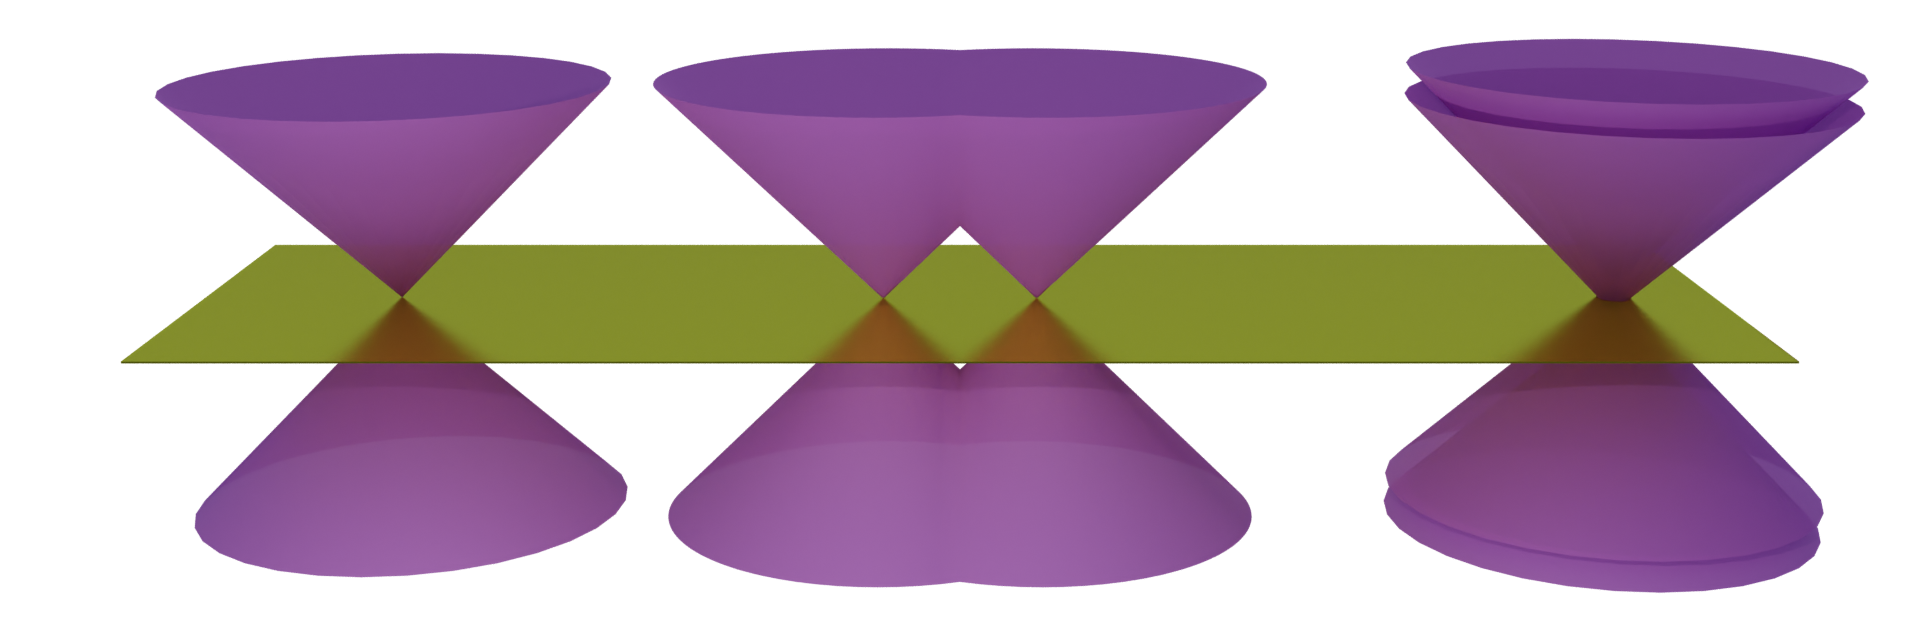
\includegraphics[width=\textwidth]{figures/cones-types-col1-opaque.png}
  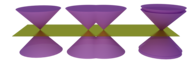
\includegraphics[width=\textwidth]{figures/cones-types-col1-opaque-small.png}
  \caption{Dispersion curves in the $k_z, k_x$-plane. \textbf{(Left)} Dirac material with superimposed cones. \textbf{(Center)} Time reversal symmetry broken, giving a Weyl material with the cones separated in momentum  space. \textbf{(Right)} The cones shifted in energy, givng a nodal loop.
    \todo{Consider making middle one with mass term.}
  }
  \label{fig:conetypes}
\end{figure}

\begin{figure}[p!]
  \centering
  % \includegraphics[width=0.75\textwidth]{figures/tilt_cone}
  % \includegraphics[width=0.75\textwidth]{figures/conesTransparent-verysmall.png}
  % 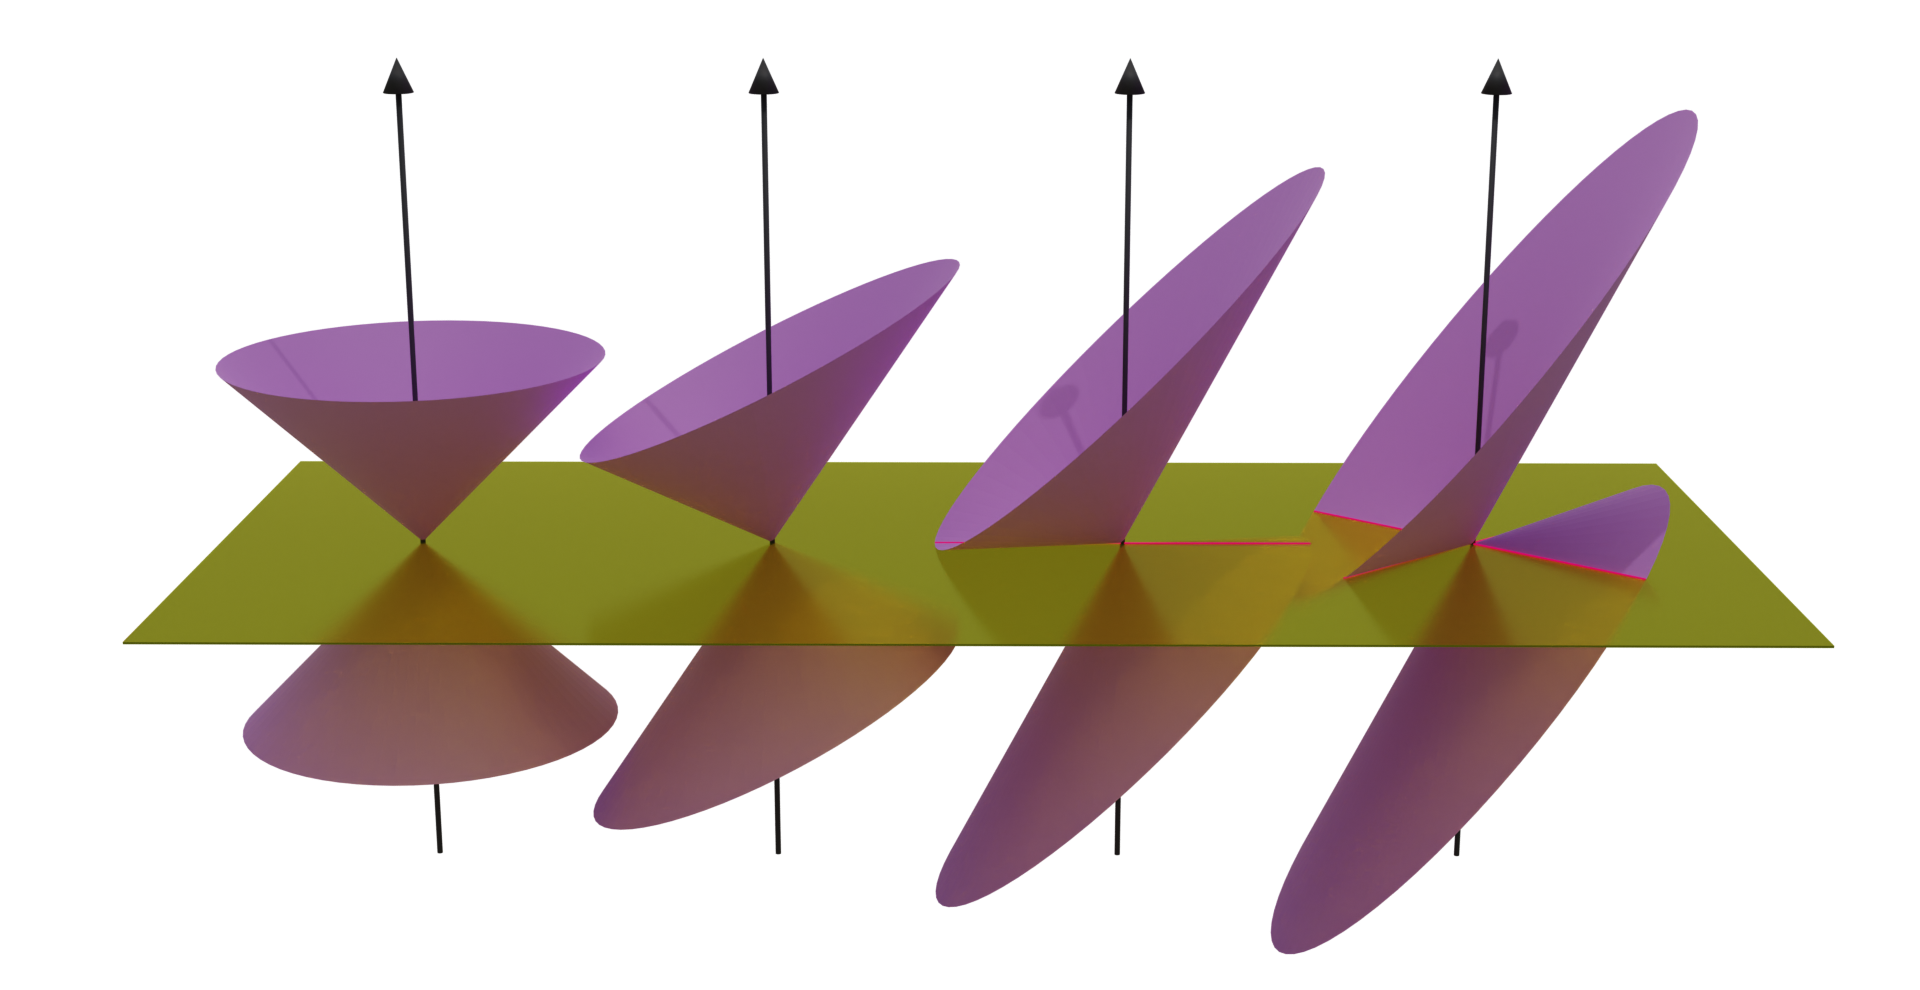
\includegraphics[width=\textwidth]{figures/cones-tilt-color1.png}
  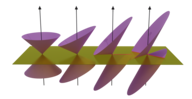
\includegraphics[width=\textwidth]{figures/cones-tilt-color1-small.png}
  \caption{Tilted Dirac cones.
    From left to right the tilt increases, from no tilt in the first cone to overtilt in the last.
    The three first are Type-I Weyl semimetals, the last is a Type-II semimetal.
    The Fermi surface is marked in red.
    See main text for details.
    \label{fig:tilted-cones}
  }
  % \caption{Tilted cone. \textbf{(Left)} Type I Weyl semimetal, with no tilt.
  %   \textbf{(Center)} Type  I Weyl semimetal, with tilt.
  %   \textbf{(Right)} Type II Weyl semimetal, meaning the tilt makes the upper part of the cone go below horizontal.}
  \label{fig:tiltcone}
\end{figure}

\subsection{Chern number of the Weyl point}\label{sec:chern-number-weyl}
In order to more explicitly demonstrate the topological nature of the tilted Weyl cone in Eq.~(\ref{eq:3}), we will find a non-zero topological invariant associated with that state.
Thereby showing that the material is a topological material.
The topological number we will calculate is the Chern number, related to the Berry curvature of the bands in some enclosed surface.
In order to calculate the Chern number, we must first find an expression for the Berry curvature of our system.
This derivation will follow closely Berry's original derivation~\cite{berryQuantalPhaseFactors1984} of the Berry phase of a two-level system with the Hamiltonian
\begin{equation}
  \label{eq:6}
  H(\vec{R}) = \frac12 \vec\sigma \vec{R}.
\end{equation}
Some notation has been modernized with inspiration from the treatment of the Berry phase of the spin-$1 /2$ particle in an external magnetic field in~\citeauthor{holsteinAdiabaticTheoremBerry1989}~\cite{holsteinAdiabaticTheoremBerry1989}.

Suppose we have a Hamiltonian $H(t)$, and that its $t$-dependence can be parameterized by $\vec{R} = \vec{R}(t)$, as in $H(t) = H(\vec{R}(t))$.
Any evolution of the Hamiltonian through time, may then be described as a geometric path through the $\vec{R}$-space.
As the reader might be aware, Berry's most famous discovery was that a closed path through $\vec{R}$-space gives an observable phase to the system, unlike the non-physical dynamical phase, which may be removed by a suitable choice of gauge.
Here we will however focus on the so-called Berry curvature, $\vec{B}$, a vector field which will be shown to be useful in the categorization of topological materials.
Note that there is some variation in the literature on the naming of the various quantities, and the sign convention used.
In particular, the word Berry curvature will in some literature refer to a rank two tensor, while our quantity $\vec{B}$ is referred to as the Berry field strength.
In particular, if we let the rank two tensor be denoted $F_{ij}$, the Berry field strength $\vec{B}$ is given by
\begin{equation}
  B_i = \epsilon_{ijk} F_{jk}.
\end{equation}
\todo{Consider rewriting some of  this. Look in topology book}
The Berry curvature for the state $n$ is explicitly defined as~\cite{berryQuantalPhaseFactors1984}
\todo{Should we add some more comments about adabiatic? See topo book}
\begin{equation}
  \vec{B_n}(\vec{R}) =
  -\Im \sum_{m\neq n}
  \frac{
    \braket{n(\vec{R}) | \nabla_{\vec{R}} H | m(\vec{R}) }
    \times
    \braket{m(\vec{R}) | \nabla_{\vec{R}} H | n(\vec{R}) }
  }{
    (E_m(\vec{R}) - E_n(\vec{R}))^2
  },
\end{equation}
where $\times $ denotes the cross product.
Notice that for a degeneracy $E_n = E_m$ there will be an infinity in $\vec{B_n}$.
Considering the Berry curvature as a field in $\vec{R}$-space, this resembles a source, as will become relevant later.
This may now be applied to for example the Weyl semimetal, both in the interest of solidifying the above theory, and as it will be useful in future  consideration.

The Hamiltonian around the (untilted) Weyl point is
\begin{equation}
  H = v_F \vec{\sigma} \cdot \vec{p},
\end{equation}
with $v_F$ the Fermi velocity, $\vec{\sigma}$ the Pauli matrices, and $\vec{p}$ the momentum operator.
% \todo{Now suddenly R is not dependent  on t??}
By letting $\vec{R} = v_F \vec{p}$, the Berry curvature of the Hamiltonian can be found.
The eigenvalues of this system are
\begin{equation}
    E_+ = -E_-
    = |R|.
\end{equation}
The aforementioned degeneracy is here of course the Weyl point, where $E_+ = E_- = 0$.
Noting that
\begin{equation}
  \label{eq:gradHamil}
  \nabla_{\vec{R}} H = \vec\sigma,
\end{equation}
we can calculate the Berry curvature easily.
Denote by $\ket{+}$ the state with the eigenvalue $E_+$ and $\ket{-}$ the state with the eigenvalue $E_-$.
Take also, without loss of generality, $\vec{R}$ to be in the $z$-direction.
This gives
\begin{equation}
  \vec{B}_+ = -\Im
  \frac{
    \braket{+ | \vec\sigma | -}
    \times
    \braket{- | \vec\sigma | +}
  }{
    4 R^2
  }.
\end{equation}
As $\ket{+}$ and $\ket{-}$ are eigenstates of $\sigma_z$ and orthogonal to each other, only the $z$-component of the cross product may contain non-zero contributions.
\begin{equation}
  \begin{split}
    \vec{B}_+ &= - \frac{\hat{z}}{4 R^2}
    \Im \left(
    \braket{+ | \sigma_x | -}
    \braket{- | \sigma_y | +}
    -
    \braket{+ | \sigma_y | -}
    \braket{- | \sigma_x | +}
    \right)\\
    &= - \frac{ \hat{z}}{2 \vec{R}^2}.
  \end{split}
\end{equation}
Here, the effect of the Pauli matrices on the eigenvectors was used, according to
\begin{align}
  \sigma_x \ket{\pm} &= \ket{\mp}\\
  \sigma_y \ket{\pm} &= \pm i \ket{\mp}
\end{align}
Returning to general axis orientations, one has
\begin{equation}
  B_+ = - \hat{R} / 2\vec{R}^2 = - \vec{R} / 2 \vec{R}^3.
\end{equation}
For the $\ket{+}$-band, the Weyl point thus takes the form of a negative monopole in $R$-space;
this motivates the requirement that Weyl points must always appear in pairs of opposite chirality, as the divergence of the Berry curvature must always be zero over the entire sample.
\todo{There should probably be some care taken here with the sign of $v_F$.}

Extending the calculation to a tilted Weyl cone
\begin{equation}
  H = v_F \vec{\sigma} \cdot \vec{p} + v_F \vec{t} \cdot \vec{p},
\end{equation}
is trivial.
The energies gain a factor \( v_F \vec{t}\cdot \vec{p} = \vec{t} \cdot \vec{R}\), however, this does not change the difference between the energies of the states.
Furthermore, the gradient of the Hamiltonian, Eq.~\eqref{eq:gradHamil}, gains a factor
\begin{equation}
  \nabla_{\vec{R}} H = \vec\sigma + \vec{t},
\end{equation}
which does not affect the result, as \( \braket{\pm | \vec{t} | \mp} = 0 \).

As mentioned, the Chern number is one of several numbers that is used to classify topological materials.
The Chern number is defined as
\begin{equation}
  C = \frac{1}{2\pi} \oint_{\partial C} \vec{B_+} \cdot \mathrm{d}\vec{S},
\end{equation}
where the integral is taken over the closed surface $\partial C$, enclosing the volume $C$.
Noting that the Berry curvature has the shape of a monopole source at $\vec{p} = 0$, we immediately know the value of this quantity from electromagnetism.
We will, however, carry out the computation explicitly here.
With the divergence theorem in mind, it behooves us to find the divergence of the Berry curvature.
This divergence is zero everywhere except in the monopole source, giving
\begin{equation}
  \nabla \cdot \vec{B_+} = -\frac12 \nabla \cdot \hat{R} / R^2 = -2 \pi \delta(\vec{p}),
\end{equation}
where $\delta$ is the Dirac delta distribution.
By virtue of the divergence theorem the Chern number is then found to be
\begin{equation}\label{eq:chern}
  C = \frac{1}{2\pi} \int_C \nabla \cdot \vec{B_+} \mathrm{d} C = -1,
\end{equation}
where the property of integrals over Dirac delta distributions was used.

Note that some literature will have a Chern number differing from \eqref{eq:chern} by the sign of the Fermi velocity,
\begin{equation}
  C = - \operatorname{sign}(v_F).
\end{equation}
This simply comes from the definition of the eigenstates.
We have put the sign dependence in the state, making the $E_+$ state always have positive eigenenergy.
In literature that instead defines $E_+ = v_F |R|$ the state's energy will depend on the sign of the Fermi velocity, and as a consequence, the sign dependence will end up in the Chern number instead.

The overall divergence of Berry curvature must be zero, or equivalently, the sum of the Chern numbers must be zero.
The Hamiltonian Eq. (\ref{eq:6}) chosen with the opposite chirality,
\begin{equation}
  H(\vec{R}) = -\frac{1}{2} \vec{\sigma} \vec{R},
\end{equation}
has the opposite Berry curvature, and also the opposite Chern number.
Thus, Dirac cones must appear in pairs of opposite chirality, either superimposed as the Dirac semimetal case or separated in momentum space, as the Weyl semimetal.

In light of the interpretation of the Dirac point as a monopole of Berry curvature, the discussion in section~\ref{sec:weyl-dirac-cones}, on page \pageref{sec:stability-of-gap}, on the stability of the band crossing in two and three dimensions gets an intuitive and geometric interpretation.
In Figure~\ref{fig:curvature_plane} the Berry curvature pole is shown in $p$-space, together with a plane parallel to the $xy$-plane, which we will denote the \emph{state plane}.
In the two-dimensional case, the state is confined to the state plane, with the $z$-position of the plane given by any mass terms $m \sigma _z$.
In the three-dimensional case, the state is not confined to this plane, as the parameter $p_z$ is a free variable, or alternatively it may be considered as a freedom to move the state plane freely, with its initial position simply shifted by any mass terms.
It is thus obvious that one may never reach the monopole in the two-dimensional case, and thus for no $\vec{k}$ is there a band crossing.
Importantly, the Berry curvature is indeed non-zero, however any closed  curve of integration will give a Chern number of zero;
the  monopole has been moved outside the dimensionality of freedom.
\begin{figure}[ht]
  \centering
  % 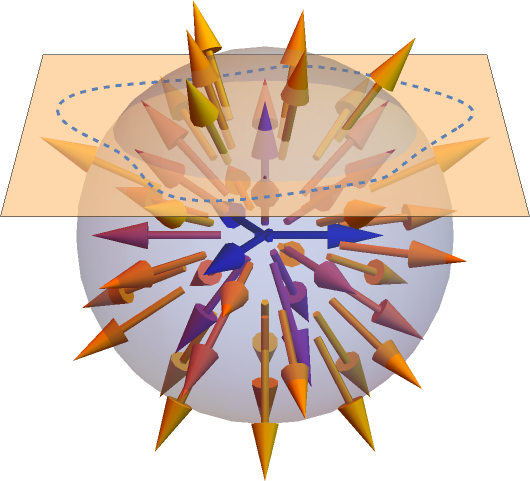
\includegraphics[width=0.5\textwidth]{figures/berryCurvePlanewpath.png}
  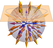
\includegraphics[width=0.5\textwidth]{figures/berryCurvePlanewpath-small.png}
  \caption{The state plane, transparent yellow, parallel to the $xy$-plane and a Berry curvature monopole at the origin.
  An integration contour is shown in blue dashed.
  See main text for details.}
  \label{fig:curvature_plane}
\end{figure}


% \begin{figure}[ht]
%   \centering
%   \begin{tikzpicture}
%     \coordinate (O) (0,0,0);
%     \draw[->] (O) -- (5,0,0); 
%     \draw[->] (O) -- (0,5,0); 
%     \draw[->] (O) -- (0,0,5); 

%     \def\N{9}
%     \foreach \n in {0,...,\N}
%     {
%       \foreach \t in {0,...,\N}
%       {
%         \draw[->] (xyz spherical cs:radius=1.5,latitude={\n*360/\N},longitude={\t*360/\N}) -- (xyz spherical cs:radius=2,latitude={\n*360/\N},longitude={\t*360/\N});
%       }
%     }
%     \begin{scope}[canvas is zx plane at y=1.7,fill=red]
%       \draw[help lines, opacity=0.7] (-2,-2) grid (2,2);
%       \draw [cyan,thick] plot [smooth cycle] coordinates { (-1,0) (1,1) (1,-2) (0,-1) (-1, -1)};
%       \node[transform shape, rotate=90, yscale=2] at (-1.7,1.5) {$z = 2$}; 
%     \end{scope}
%   \end{tikzpicture}
%   \caption{todo}
% \end{figure}

\begin{comment}
%%%%   Old text, probably to be deleted %%%%%
\newpage

While the nearly free quasi-particle model performs very well for most metals, with the Hamiltonian $\frac{p^2}{2m^*}$, this models fails for the Dirac-materials.
Instead of obeying the Schrödinger equation as most materials, they obey a Dirac equation with the speed of light being replaced by the Fermi velocity $v_F$.
$$
H_D = v_F \sigma p + m v_F^2 \sigma_z.
$$
Here the spin degree of freedom $\sigma$ is either from the actual spin of the particle or some pseudo-spin degree of freedom such as a bipartite lattice.

The origin of this form for the Hamiltonian varies for different materials.
For graphene, for example, this form of the Hamiltonian follows directly from the tight binding model with a bipartite lattice.
Notice, however, that the spin degree of freedom in this case does not come from the actual spin of the particle, but is rather a pseudo spin degree of freedom coming from the effective two level system that appears as a result of the two positions in each cell.

The band structure of the Hamiltonian is easily found.
Writing out the Hamiltonian, setting $v_F=1$ for simplicity, we get
\begin{equation}
  H_D = p_x \sigma_x + p_y\sigma_y + m \sigma_z,
\end{equation}
which has eigenvalues at
$$
| H_D - E I | = 0.
$$
This gives us the solutions
\begin{equation}
  E = \pm \sqrt{
    k_x^2 + k_y^2 + m^2
  }.
\end{equation}

Just as in the particle physics case, the Dirac equation will exhibit gapless band structures as $m\rightarrow 0$.
As introducing a term $m\sigma_z$ would break inversion symmetry, such systems cannot be gapped.
One may show that in graphene, time and inversion symmetry will force the mass term to be zero, and the gap disappears.
\end{comment}
\begin{comment}
  \begin{figure}
    \begin{tikzpicture}
      \begin{axis}[
        legend style={
          at={(0.5, 0.95)},
          anchor={north},
        },
        legend cell align=left,
        width=13cm,
        cycle list name=linestyles,
        domain=-pi/2:pi/2,
        samples=201,
        ]
        \pgfplotsset{cycle list shift=-1}
        \foreach \m in {0, 0.1, 1, 2} {
          \addplot+[forget plot] {sqrt(x^2 + \m^2)};
          \addplot+ {-sqrt(x^2 + \m^2)};
          \addlegendentryexpanded{$m=\m$}
        }
      \end{axis}
    \end{tikzpicture}
    \caption{Band structure for the 2D Weyl Hamiltonian for various values of the mass term.} 
  \end{figure}
\end{comment}

\clearpage
% \section{Type II Weyl semimetals}
\subsection{Tilted Dirac semimetals}
\label{sec:typeii}
% \setlength{\wrapoverhang}{\marginparwidth}
% \addtolength{\wrapoverhang}{\marginparsep}
% \addtolength{\wrapoverhang}{-1cm}
\begin{wrapfigure}[15]{r}{.25\textwidth}
  \centering
  \vspace{-2.6em}
  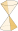
\includegraphics[width=.25\textwidth]{figures/conicSection}
  \setcapindent*{0pt}
  \caption{The conic section. \label{fig:conic-section-sketch}}
\end{wrapfigure}
The conic section problem with the intersecting plane restricted to pass through the node of the cone is trivially seen to have two solutions: a point and two intersecting lines, shown schematically in \cref{fig:conic-section-sketch}.
Despite this, the possibility of a Weyl cone tilted beyond the Fermi level was never considered before \textcite{soluyanovTypeIIWeylSemimetals2015} described this new class of Weyl semimetals in 2015.
This now seemingly obvious possibility made an already rich field even more exciting, opening up for a wider range of novel and interesting effects~\cite{soluyanovTypeIIWeylSemimetals2015,sharmaChiralAnomalyLongitudinal2017,yuPredictedUnusualMagnetoresponse2016,tchoumakovMagneticFieldInducedRelativisticProperties2016,ferreirosAnomalousNernstThermal2017}.

% \begin{figure}[ht]
%   \centering
%   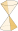
\includegraphics[width=0.25\textwidth]{figures/conicSection}
%   \caption{Sketch of the conic section with the plane passing through the node of the cone. The intersection surface is either a point at the node or two intersecting lines. \label{fig:conic-section-sketch}}
% \end{figure}

In this section, we investigate in more detail the tilted Weyl cone, the star of this thesis.
The tilted Hamiltonian was introduced in \cref{eq:hamil-tilt-isotropic}
\[
H_s = s v_F \vec{\sigma} \vec{p} + v_F \vec{t}^{s} \vec{p},
\]
where we chose isotropic Fermi velocity.
As discussed earlier, the proper Dirac equation of particle physics cannot include such a tilting term, as it obviously breaks Lorentz invariance.
The emergent Dirac equation of condensed matter physics, however, need not respect the Lorentz invariance and such a tilting term is no problem.
\todo{I am pretty sure there is some neat analogy here that should be included. Light cone etc.}

As was alluded to in the introduction to the section, the Weyl cone has two distinct phases: Type-I and
Type-II.
Tilting the Weyl cone, the upper and lower bands will at some tilt angle touch the Fermi level, a \emph{critical} tilt.
Going beyond this, the upper (lower) band dips below (above) the Fermi level, and we have what is known as a Type-II Weyl semimetal.
Although the two states are similar in many ways, they also have hugely important differences separating them from one another.
In the Type-I regime, the density of states goes to zero at the Fermi level.
In the Type-II regime, however, particle and hole pockets appear -- the intersection of the cone and the Fermi level goes from a singular point to two infinite lines (shown in \cref{fig:tilted-cones} on page \pageref{fig:tilted-cones}).
This abrupt change of the topology of the Fermi surface, from closed to open, is known as a Lifshitz transition \cite{volovikTopologicalLifshitzTransitions2017}.
This gives Type-II Weyl semimetals manifestly different properties from Type-I, useful both in practical applications and as an interesting phenomenon seen from a purely scientific perspective.

% In the case of massless fermions, the particle physics equivalent of the Weyl semimetal, such a tilt is not possible, due to the requirement of Lorentz invariance \todo{add cite or explain}.
% In condensed matter physics, however, this is not an issue, and it is indeed a real class of materials \todo{cite examples}.
% We denote these types of materials Type-II Weyl semimetals, as opposed to Type-I.
% The transition between Type-I and Type-II is abrupt -- the Fermi surface goes from a single point to two intersecting lines, in other words going from a zero dimensional to a one dimensional surface.
% \todo{Make sure this is indeed a one dimensional surface. It is kind of 1DxZ(2)}
% \todo{Make sure it is one dim also for the 3D case, quadric surface, not conic intersection}
% Type-II also has electron and particle pockets at the Fermi level.
% While the density of states for a Type-I semimetal goes to zero as one approaches the Fermi level, this causes Type-II to have a finite density of states at the Fermi level.
% \todo{End with something like: all in all this gives type ii weyl semimetal manifestly different properties from tyep i, useful both in practical applications and as an interesting phenomena seen from a purely scientific perspective}

\subsubsection{Linear Dirac equation from tight binding model}
\label{sec:tilt:tightbindingmodel}
We will firstly consider a slightly more realistic tight binding toy model for a Weyl semimetal, with a parameter taking the system from a Type-I to a Type-II.
This is instructive both in order to more intuitively see the origin of the terms causing the tilting of the Dirac cone, and also to discuss the validity of the linear model in different contexts.
We will linearize the model around the Weyl points, regaining the familiar form of a Dirac cone, with an additional anisotropy term causing the tilt.

We will use the general time-reversal breaking model described by \textcite{mccormickMinimalModelsTopological2017}
\begin{equation}
  \begin{split}
    H(\vec{k}) &= \left[ ( \cos k_y + \cos k_z - 2 )m - 2 t (\cos k_x - \cos k_0) \right] \sigma_1\\
    &\pe - 2 t \sin k_y \sigma_2 - 2t \sin k_z \sigma_3
    + \gamma (\cos k_x - \cos k_0),
  \end{split}
\end{equation}
where \( t \) must not be confused with the tilt term of the linear model.
There are Weyl nodes at \(\vec{K}' = (\pm k_{0}, 0,0)\), and the parameter $\gamma$ controls the tilting of the emerging cones.
For \( k_0 = \pi /2 \), the cones are isotropic in low-energy expansion.
As \( k_0 \) is reduced, the cones are brought closer together and made anisotropic, as the effective Fermi velocity is not the same in the \( x \) and \( y \) direction, as shown in \cref{fig:typeii:move-nodes}, where two cones are moved until they meet at the origin.
% \cref{fig:ridgeline} shows the cross section \(k_{y} = 0\) of the eigenvalues of this system, as \(\gamma\) is gradually increased from 0 to 0.15 \todo{verify numbers}.
\cref{fig:typeii:bendbands} shows the eigenvalues of the system, as \( \gamma \) is increased from 0 to \( 3t \).
A value of $\gamma=0$ gives no tilt, while for $\gamma > |2 t|$ the Type-II system emerges.
The \(\gamma\)-term ``warps'' the bands, and in the limit of Type-II the hole band crosses the Fermi level into positive energy, while the particle band crosses the Fermi level into negative energies.
We call these electron and hole pockets, respectively.
Note that in this model, the pockets are shared between the two nodes.
One may also construct tight binding models with isolated pockets \cite{mccormickMinimalModelsTopological2017}.

\begin{figure}[p]
  \centering
  \begin{subcaptionblock}[t]{\textwidth}
    \centering
    % 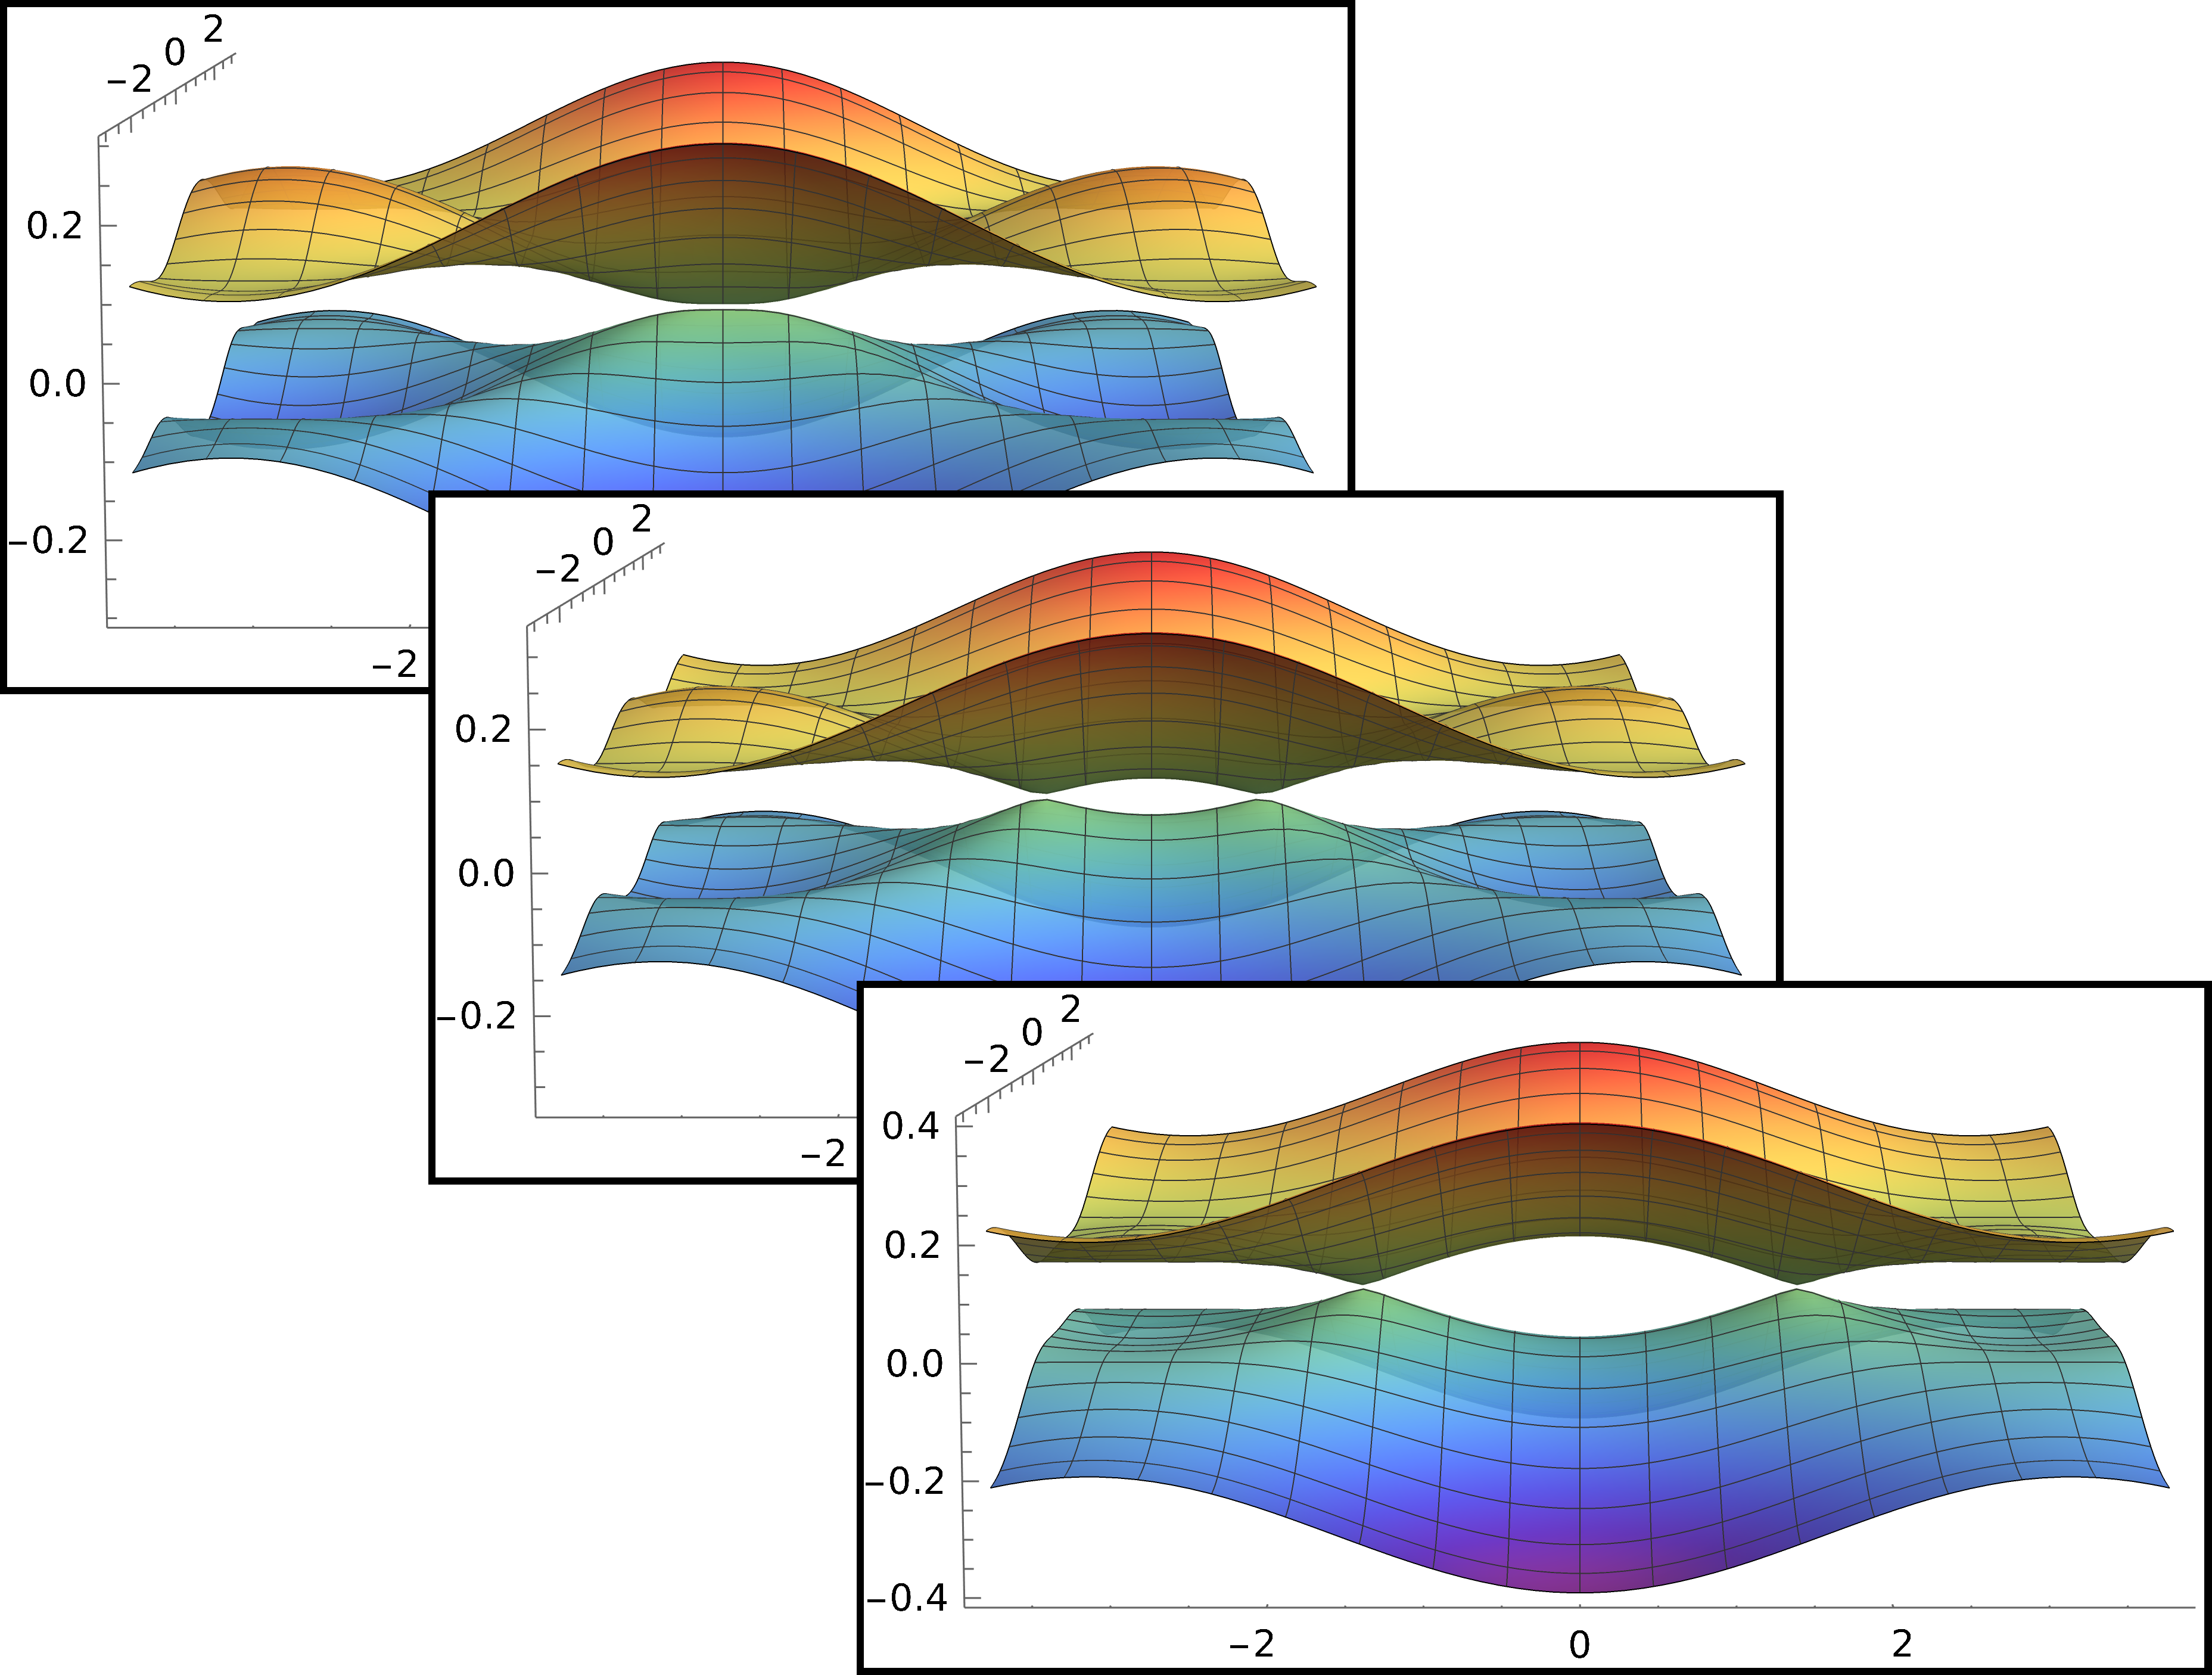
\includegraphics[width=0.7\textwidth]{figures/movetypeiinode}
    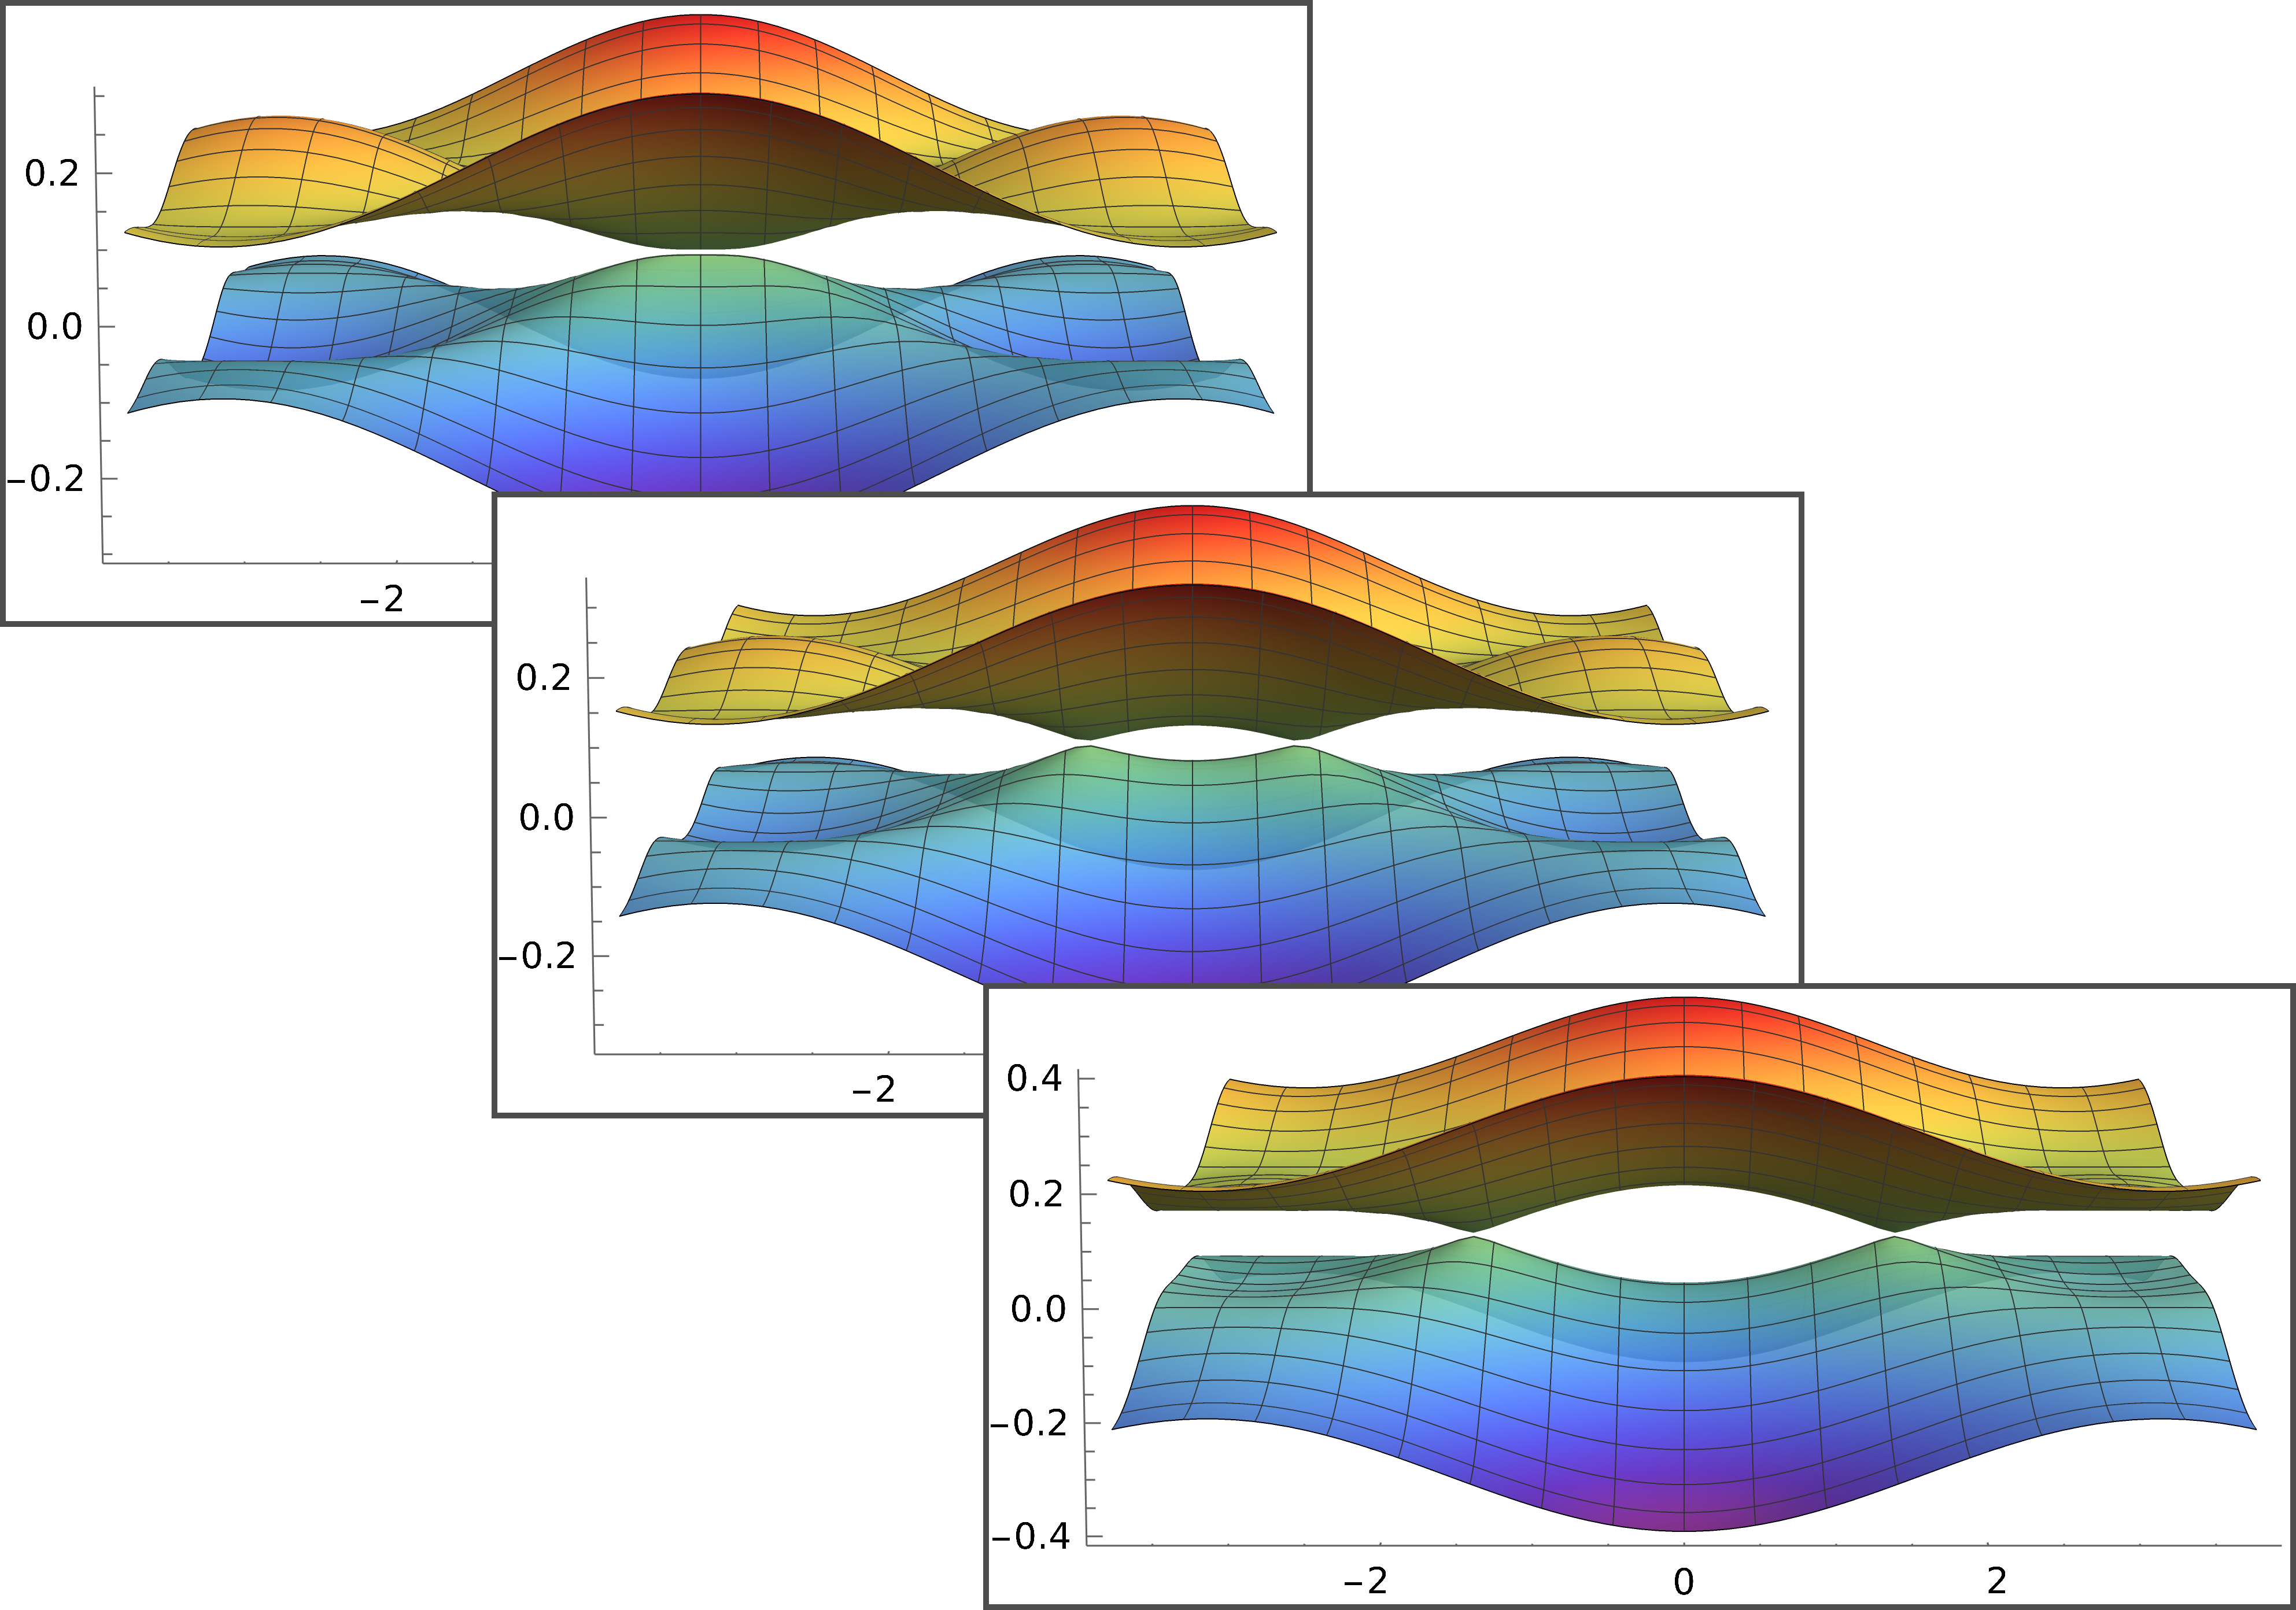
\includegraphics[width=.7\textwidth]{figures/typeIImoveTransition}
    \caption{\label{fig:typeii:move-nodes}A Type-I Weyl semimetal with separation between the nodes \(2k_{0} = 0, \pi/2, \pi \).}
  \end{subcaptionblock}
% \end{figure}
% \begin{figure}[!htb]
  \begin{subcaptionblock}[t]{\textwidth}
    \centering
    % \vspace{1em}  % More space to fig above
    \medskip
    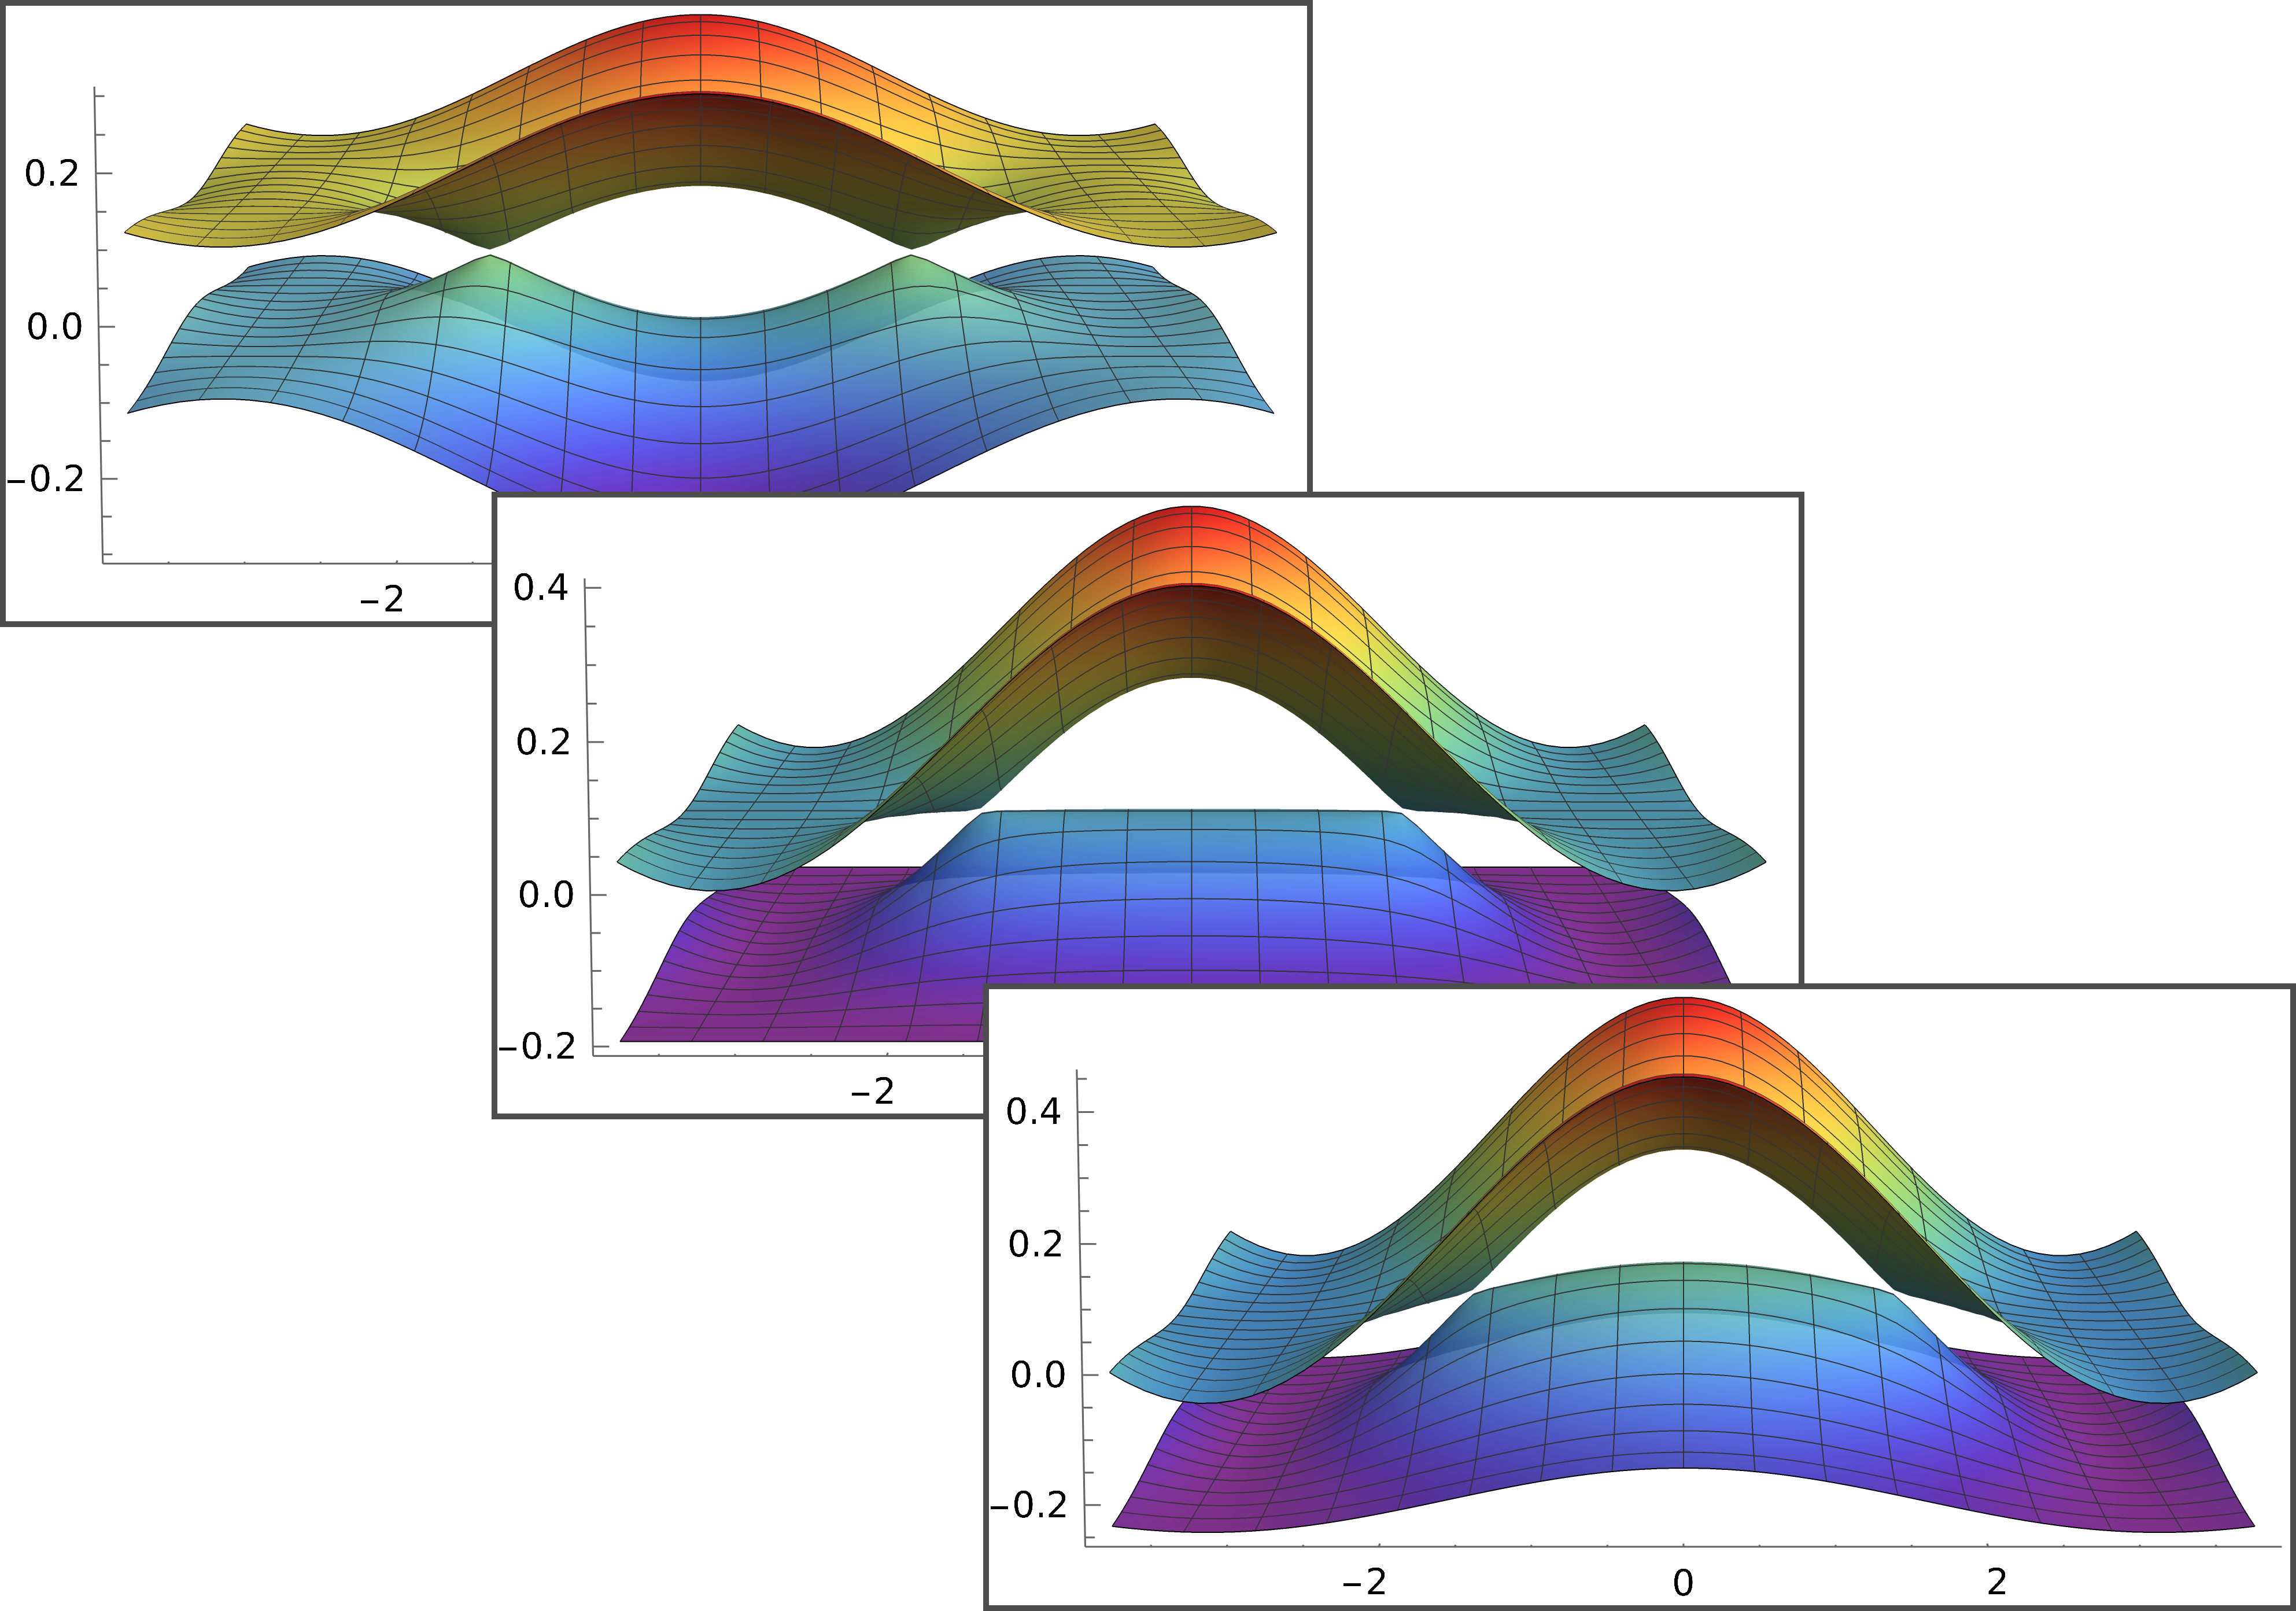
\includegraphics[width=.7\textwidth]{figures/bendingTransition.png}
    \caption{\label{fig:typeii:bendbands}The ``warping'' parameter \( \gamma \) increased from left to right, %
      \( \gamma = 0, 2 t, 3 t \), %
      transitioning the system from Type-I to Type-II.}
  \end{subcaptionblock}
  \caption{Two-band tight binding model for a tilted Dirac semimetal.
    Shown are the two energy bands plotted in the \( xz \)-plane in momentum space;
    the separation of the nodes is in the \( x \)-direction.
    In \subref{fig:typeii:move-nodes} the separation between the two nods is adjusted.
    In \subref{fig:typeii:bendbands} the bands are ``warped'' to induce tilt.
    See main text for details of the model.
  }
\end{figure}

Linearizing around the Weyl nodes the Hamiltonian reduces to the familiar expression of a Dirac cone
\begin{equation}
  \label{eq:7}
  H(\vec{K} ^{'\pm} + \vec{k}) \approx \mp 2 t k_{x} \sin k_{0} \sigma_{1} - 2 t (k_{y} \sigma_{2} + k_{z} \sigma_{3}) \mp \gamma k_{x} \sin k_{0} \sigma_{0}, \: k_{x}, k_{y}, k_{z} \ll 1.
\end{equation}
When the separation between the two nodes is \(\pi\), i.e. \(k_{0} = \pi/ 2 \), the linearized Hamiltonian around the cone is
\begin{equation}
  \label{eq:8}
  H'(\vec{k}) = \mp 2 t k_{x} \sigma_{x} - 2t k_{y} \sigma_{y} - 2 t k_{z} \sigma_{z} \mp \gamma k_{x},
  % h'(\vec{v}) = -2t \vec{k} \vec{\sigma} - \gamma k_{x}.
\end{equation}
with \( \mp \) corresponding to the node at \( \vec{K}^{' \pm} \).
For a system
\begin{equation}
  \label{eq:155}
  H = \gamma_i k_i + k_i A_{ij} \sigma_j,
\end{equation}
the chirality of the node \( s = \det(A_{ij}) \) \cite{mccormickMinimalModelsTopological2017}, and we see this gives a negative cone at \( k_x = \pi /2 \) and positive at \( k_x = -\pi /2 \).
We could arrive at a more familiar form of the expression by letting \( 2 t \to v_F, \gamma \to v_F t \), and do a \( \pi \) rotation around \( x \) at the positive cone, giving
\begin{equation}
  \label{eq:158}
  H'^{s}(\vec{k}) = s v_F \vec{k} \cdot \vec{\sigma} + s v_F t k_x.
\end{equation}
The model thus gives rise to a pair of Weyl cones, with an inversion symmetric tilt, i.e. they tilt with equal magnitude in the opposite direction.
Moving the two nodes closer together, the effective Fermi velocity in the \(x\)-direction is rescaled, and the system is anisotropic even for no tilt (\(\gamma=0\)).
As discussed earlier, this may be mitigated by a rescaling of \( k_x \).

% \begin{figure}[ht]
%   \centering
%   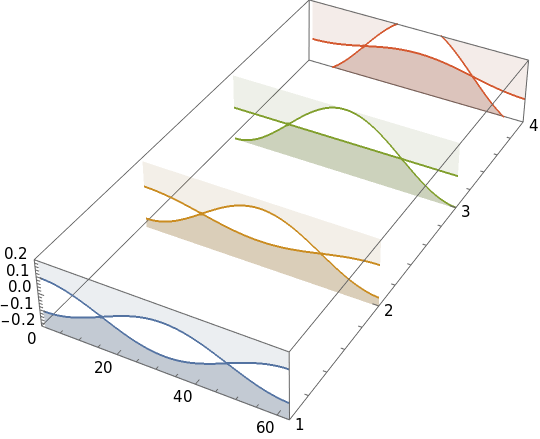
\includegraphics[width=0.7\textwidth]{figures/typeIIridgeline}
%   \caption{The values of the parameters were chosen to be \(m=0.15, t=-0.05, \) and \(2 k_{0}=\pi\).\label{fig:ridgeline}\todo{Write this}}
% \end{figure}

% \begin{figure}[ht]
%   \centering
%   \tikzsetnextfilename{ridgeline}
%   \begin{tikzpicture}
%     \pgfplotscreateplotcyclelist{myexotic}{
%       teal,fill=teal!80!black\\
%       orange,fill=orange!80!black\\
%       cyan!60!black,fill=cyan!80!black\\
%       lime!80!black,fill=lime\\
%       red,fill=red!80!black\\
%       yellow!60!black,fill=yellow!80!black\\
%       black,fill=gray\\
%       red,fill=red!80!black\\
%     }
%     \begin{axis}[
%       area plot/.style={
%         fill opacity=0.75,
%         % draw=#1!80!black,thick,
%         % fill=#1,
%         mark=none,
%       },
%       cycle list name={myexotic},
%       plot box ratio=3 5 1,
%       view={-40}{20},
%       zmin=-0.2, zmax=0.2,
%       xlabel=\( k_x \),
%       ylabel=\( \gamma \),
%       zlabel=Energy,
%       xtick={-3.1415,-1.5708,0,1.5708,3.1415},
%       xticklabels={\( -\pi \), \( -\frac{\pi}{2} \), 0, \( \frac{\pi}{2} \), \( \pi \)},
%       ytick={1,2,3,4},
%       yticklabels={0,0.05,0.1,0.15},
%       ]

%       % \addplot3[area plot=orange] table[z index=1, y expr=1, col sep=comma] {data/tightBindModel-topbottom.csv};
%       % \addplot3[area plot=orange] table[z index=2, y expr=1, col sep=comma] {data/tightBindModel-topbottom.csv};

%       % \addplot3[area plot=blue] table[z index=3, y expr=2, col sep=comma] {data/tightBindModel-topbottom.csv};
%       % \addplot3[area plot=blue] table[z index=4, y expr=2, col sep=comma] {data/tightBindModel-topbottom.csv};

%       % \addplot3[area plot=teal] table[z index=5, y expr=3, col sep=comma] {data/tightBindModel-topbottom.csv};
%       % \addplot3[area plot=teal] table[z index=6, y expr=3, col sep=comma] {data/tightBindModel-topbottom.csv};

%       % \addplot3[area plot=teal] table[z index=7, y expr=4, col sep=comma] {data/tightBindModel-topbottom.csv};
%       % \addplot3[area plot=teal] table[z index=8, y expr=4, col sep=comma] {data/tightBindModel-topbottom.csv};


%       \addplot3+[forget plot, area plot=teal] table[z index=7, y expr=4, col sep=comma] {data/tightBindModel-topbottom.csv};
%       \addplot3+[area plot=teal] table[z index=8, y expr=4, col sep=comma] {data/tightBindModel-topbottom.csv};

%       \addplot3+[forget plot, area plot=teal] table[z index=5, y expr=3, col sep=comma] {data/tightBindModel-topbottom.csv};
%       \addplot3+[area plot=teal] table[z index=6, y expr=3, col sep=comma] {data/tightBindModel-topbottom.csv};

%       \addplot3+[forget plot, area plot=blue] table[z index=3, y expr=2, col sep=comma] {data/tightBindModel-topbottom.csv};
%       \addplot3+[area plot=blue] table[z index=4, y expr=2, col sep=comma] {data/tightBindModel-topbottom.csv};

%       \addplot3+[forget plot, area plot=orange] table[z index=1, y expr=1, col sep=comma] {data/tightBindModel-topbottom.csv};
%       \addplot3+[area plot=orange] table[z index=2, y expr=1, col sep=comma] {data/tightBindModel-topbottom.csv};
%     \end{axis}
%   \end{tikzpicture}
%   \caption{The values of the parameters were chosen to be \(m=0.15, t=-0.05, \) and \(2 k_{0}=\pi\).\label{fig:ridgeline2}\todo{Write this add ref}}
% \end{figure}


The linearized model is accurate in describing low energy interactions around the Fermi level.
For higher energies, its validity falls apart, and more complex models are warranted.
For our calculations, we will take the linear model to be sufficient.
It is much easier to work with and sufficient in most cases.

\label{sec:tilt:fermisurface-paragraph}
One of the most obvious differences between the tight binding model and the linear model is the finiteness of the former.
This is particularly important with regard to two aspects: the Dirac sea and the topology of the Fermi surface.
In high energy physics, the Dirac sea is infinitely deep \cites{burkovTopologicalSemimetals2016,vozmedianoTheoreticalPhysicsColloquium2021}, whereas, in condensed matter physics, it is not.
As is seen from the tight binding model, the Dirac sea of the two cones is really connected;
this has consequences for, among others, the interpretation of the chiral anomaly.
In our context, also the topology of the Fermi surface is of importance.
As mentioned, in the Lifshitz transition from Type-I to Type-II, the Fermi surface goes from being closed to open in the linear model.
This is not the case in the tight binding model, whose Fermi surface is shown in \cref{fig:fermiSurfaceTight}.
According to \textcite{ferreirosAnomalousNernstThermal2017} the linear model will be able to give qualitatively correct results for Type-II in the deep tilt limit.
We propose yet another argument for this claim here.
Consider again the Fermi surface in \cref{fig:fermiSurfaceTight};
as the tilt is increased the Fermi surface resembles more and more that of the linear model.
Although this is in no way rigorous, it gives hope that the linear model may give qualitatively valid results for Type-II materials in the deep tilt limit.

A priori, it is not obvious when and how the linear model falls short, and a critical interpretation and evaluation of results derived from it is always warranted.
It is, however, a very useful and interesting model.
One of the more obvious remedies one might consider, is a momentum cutoff, restricting the model to the region where it is the most correct, as is common in for example graphene calculations.
\todo{cite graphene}

\begin{figure}[htb]
  \centering
  \tikzsetnextfilename{fermiSurfaceTight}
  \begin{tikzpicture}
    \begin{axis}[
      every axis plot post/.append style={mark=none},
      ymin=-pi+0.01, ymax=pi-0.01, % Hide masked values
      xmin=-pi, xmax=pi,
      xlabel=\( k_x \), ylabel=\( k_y \),
      legend style={at={(0.5,1.05)}, anchor=south},
      legend columns=-1,
      cycle list={{dotted},{dashed},{dashdotted},{solid}},
      legend entries={
        \( \gamma = 2.0 t\),
        \( \gamma = 2.2 t\),
        \( \gamma = 3.0 t\),
        \( \gamma = 6.0 t\),
      },
      ]
      %% Critical tilt
      \addplot+[domain=-pi:-pi/2, blue, forget plot] {0};
      \addplot+[domain=pi/2:pi, blue, forget plot] {0};
      \addplot+[domain=-pi/2:pi/2, red, legend image post style={black}] {0};

      % \addplot[samples=100] {atan(sqrt(10)*cos(x)*sqrt(1/(27+32*cos(x)-5*cos(2*x))))};
      % CSV has a strange format
      % outer only given for positve
      \foreach \idx in {1,5,6}{
        % Upper
        \addplot+[red, forget plot] table[col sep=comma, y index=\idx] {data/fermiLevelTightInner.csv};
        \addplot+[blue, forget plot] table[col sep=comma, y index=\idx] {data/fermiLevelTightOuter.csv};
        \addplot+[blue, forget plot] table[col sep=comma, y index=\idx, x expr=-\thisrowno{0}] {data/fermiLevelTightOuter.csv};

        % Lower
        \addplot+[red, forget plot] table[col sep=comma, y expr=-\thisrowno{\idx}] {data/fermiLevelTightInner.csv};
        \addplot+[blue, forget plot] table[col sep=comma, y expr=-\thisrowno{\idx}] {data/fermiLevelTightOuter.csv};
        \addplot+[blue, legend image post style={black}] table[col sep=comma, x expr=-\thisrowno{0}, y expr=-\thisrowno{\idx}] {data/fermiLevelTightOuter.csv};
      }
      \addplot[domain=0.7:pi-0.7,gray, forget plot] {-pi/2 + x};
      \addplot[domain=0.7:pi-0.7,gray, forget plot] {pi/2 - x};
      \addplot[domain=-pi+0.7:-0.7,gray, forget plot] {pi/2 + x};
      \addplot[domain=-pi+0.7:-0.7,gray, forget plot] {-pi/2 - x};
    \end{axis}
  \end{tikzpicture}
  \caption{The Fermi surface of the tight binding model in the Type-II phase, with the Fermi surface of the linear model for \( \gamma=3t \) superimposed (gray).
    The Figure shows the \( k_x, k_y \) plane, with \( k_z = 0 \).
    Electron pockets are shown in red, hole pockets shown in blue.
    Note that the Fermi surface of the linear model is infinite, and here truncated for clarity.
  Figure inspired by \textcite{mccormickMinimalModelsTopological2017}.}
  \label{fig:fermiSurfaceTight}
\end{figure}

% In our calculations the linear models is sufficient, and much easier to work with, and we will thus mainly consider the linear model from here on.

\subsubsection{The tilt term -- symmetries and Type-I vs.\! Type-II}
% For tilted Dirac cones we will consider the Hamiltonian
% \begin{equation}
%   \label{eq:10}
%   H =  s v_F \vec{p} \vec{\sigma} + v_F \vec{t}^s \vec{p},
% \end{equation}
% where \( s \) denotes the chirality of the Dirac cone, \( v_F \) is the Fermi velocity, and \( \vec{t} \) is the \emph{tilt vector}.
% In general the Fermi velocity is anisotropic, as was the case in the general Dirac Hamiltonian given in \cref{eq:4}.
% By an anisotropic scaling of the momenta \( \vec{k} \), the system may always be mapped to an isotropic case, which we will consider here.
In this thesis, we consider the tilted Weyl cone Hamiltonian
\[
H^s = s v_F \vec{\sigma} \vec{p} + v_F \vec{t}^s \vec{p}.
\]
The tilt vector will in general depend on the chirality of the cone.
As the cones always appear in pairs, \( \vec{t}^s = s \vec{t} \) will give a system with inversion symmetry, as was the result from the tight binding model in the previous subsection.
In the case of broken inversion symmetry, we will consider the case of a tilt equal in direction and magnitude between the two cones, \( \vec{t}^s = \vec{t} \).
In short, we define
\begin{equation}
  \vec{t}^s =
  \begin{cases}
    \vec{t} & \text{broken inversion symmetry},\\
    s \vec{t} & \text{inversion symmetry}.
  \end{cases}\label{eq:11}
\end{equation}
This convention is used in most literature \cite{vanderwurffMagnetovorticalThermoelectricTransport2019,ferreirosAnomalousNernstThermal2017}.

With no magnetic field, the eigenvalues of the system are
\begin{equation}
  \label{eq:12}
  E_s(\vec{k})
  = \pm v_F |k| + v_F \vec{t}^s \vec{k},
  % = v_F \vec{t} \vec{k} \pm \sqrt{(v_{i} k_{i})^{2}}
  %
  % = |(t^{s}_i \pm 1)| \sqrt{( v_{i} k_{i})^{2}} \pm \sqrt{(v_{i} k_{i})^{2}}
  % = \sqrt{(t_{i} v_{i} k_{i})^{2}} \pm \sqrt{(v_{i} k_{i})^{2}},
\end{equation}
where in the literature the first term is sometimes referred to as the \emph{potential} term while the latter is the \emph{kinetic} term.
The definition for the system to be Type-II is that there exists a direction in momentum space for which the kinetic term dominates over the potential term \cite{soluyanovTypeIIWeylSemimetals2015}.
The \(\vec{t}\)-vector is thus a convenient tool for categorization -- if \(t > 1\) we have a Type-II, else we have a Type-I.


\begin{Proof}
  We may always rotate our coordinate system such that, without loss of generality, \(\vec{t} = t \hat{x}\).
  In that case, the first term dominates in the \(x\)-direction, when $t>1$.
\end{Proof}

% To properly investigate the symmetry properties of the system, we must consider the \(4\times 4\), not \(2\times 2\) Hamiltonian.
% While the 2x2 system does a goood job at describing a single cone, much important phsycis is lost when reducing the 4x4 Hamiltonian.
% For example, the requirement that the total Berry curvature over the entire Briolluine zone is zero is not met for the 2x2 Hamiltonian, as it describes only one cone of a certain chirality.
% The 4x4, however, includes two cones, which may in general be superimposed, thus conserving the total zero-divergence of the Berry curvature.
% As a matter of fact, the inclusion of both cones is important also for symmetry considerations.

When considering the symmetry properties of the system, we must consider the full \( 4\times 4 \) Dirac equation.
The \( 2\times 2 \) Weyl equation describing one cone does not capture the symmetries of the full system, which involve both Weyl cones.
Let
\[
  H = v_{F} \tau _{z} \otimes \vec{\sigma} \vec{p},
\]
where \(\tau \) is some pseudo spin degree of freedom, transforming like \(\vec{r}\).
This system describes two superimposed cones at the origin, with opposite chirality.
The effect of parity \(\mathcal{P}\) and time-reversal \(\mathcal{T}\) is
\begin{equation}
  \label{eq:135}
  \begin{aligned}
    \mathcal{P} \tau \mathcal{P}^{\dagger} &= -\tau, & \mathcal{T} \tau \mathcal{T}^{\dagger} &= +\tau,\\
    \mathcal{P} \sigma  \mathcal{P}^{\dagger} &= + \sigma,  & \mathcal{T} \sigma  \mathcal{T}^{\dagger} &= -\sigma, \\
    \mathcal{P} k \mathcal{P}^{\dagger} &= -k, & \mathcal{T} k \mathcal{T}^{\dagger} &= -\vec{k},
  \end{aligned}
\end{equation}
compactly summarized in \cref{tab:sign-transform}.
\begin{table}[h]
  \centering
  \begin{tabular}{lcc}
    \toprule
    & \(\mathcal{P}\) & \(\mathcal{T}\)\\
    \cmidrule{2-3}
    \(\tau \) & - & +\\
    \(\sigma \) & + & -\\
    \(p\) & - & -\\
    \bottomrule
  \end{tabular}
  \caption{The transformation rules for \( \tau, \sigma, p \) under parity~\( \mathcal{P} \) and time-reversal~\( \mathcal{T} \).
   \label{tab:sign-transform}
  }
\end{table}
Obviously then, the Hamiltonian is both time-reversal and parity invariant, as \(\mathcal{P} \mathcal{P}^{\dagger} = \mathcal{T} \mathcal{T}^{\dagger} = 1\).
Notice that as \( \mathcal{P} \tau \mathcal{P}^{\dagger} = - \tau \), the chiralities of the cones are interchanged under a parity transformation.

The tilt term takes the form \(v_F \tau_z^i \otimes \mathcal{I}_{2} \, \vec{t} \cdot \vec{p} \), where \( i=1 \) for inversion symmetric systems (\( \vec{t}^s = s \vec{t} \)) and \( i=2 \) for broken inversion symmetry (\( \vec{t}^s = \vec{t} \)).
We thus see explicitly, by applying the parity and time-reversal operators, that the term breaks time-reversal symmetry, and that we get self-consistency for the parity transformation.
This is also shown in \cref{fig:spin-struct-tilt}.

\begin{figure}[h]
  \centering
  \tikzsetnextfilename{symmetryspin}
  \begin{tikzpicture}
    \draw[->] (-4, 0) -- (4, 0) node[right] {\(k\)};
    \draw[->] (0, 0) -- (0, 4) node[right] {\(E\)};

    % vf = 1, v0 = 0.8
    \draw[blue] (-3.5, 0.7) -- (0, 0) -- (2, 3.6) node[right] {\(\ket{\uparrow}\)} coordinate[pos=0.7] (a);
    \draw[red] (3.5, 0.7) node[right] {\(\ket{\downarrow }\)} -- (0, 0) -- (-2, 3.6)
    coordinate[pos=0.7] (b);

    \draw[->] (a) -- ++(1, 0);
    \draw[->] (b) -- ++(1, 0);
  \end{tikzpicture}
  \caption{Time reversal breaking in tilted system.
    The cross-section in the tilt direction is shown, with blue showing one cone and red the other.
    Black arrows indicate spin direction, which for \(\ket{\uparrow {}}\) is parallel to  \(\vec{k}\) while for \(\ket{\downarrow {}}\) is parallel to \( -\vec{k} \).
    \label{fig:spin-struct-tilt}
  }
\end{figure}

The unperturbed Dirac Hamiltonian is Lorentz invariant, given that we consider an ``effective speed of light'', namely the Fermi velocity, instead of the actual speed of light \( c \).
Specifically, Lorentz invariance means invariance under the \emph{Lorentz group}.
The Lorentz group is the \( O(1,3) \) Lie group that conserves
\[
x_{\mu } x^{\mu } = t^2 - x^2 - y^2 - z^2,
\]
i.e. all isometries of Minkowski space.
More specifically, the group consists of all 3D rotations, \( O(3) \), and all \emph{boosts}.
A boost is a hyperbolic rotation from a spacial dimension to the temporal dimension.
If we now direct our focus at the Hamiltonian of the Dirac cone
\[
H = \pm v_{F} \vec{\sigma} \vec{p},
\]
we may easily show the Lorentz invariance of the system.
The time independent Schrödinger equation is
\begin{equation}
  \label{eq:136}
  H \ket{\psi } = E \ket{\psi } \implies (H^2 - E^2) = 0.
\end{equation}
As
\[
p^{\mu } = \left(\frac{E}{c}, \vec{p}\right),
\]
the operator in \cref{eq:136} is nothing more than
\begin{equation}
  \label{eq:137}
  H^2-E^2 = v_{F}^2 \vec{p}^2 - c^2 \left(p^0\right)^2 ,
\end{equation}
where we used the anticommutation relation
\[
\{\sigma_{i}, \sigma_{j}\} =  2 \delta _{ij}
\]
of the Pauli matrices.
Using now the effective speed of light \( c=v_F \), \cref{eq:136} is
\begin{equation}
  \label{eq:138}
  - v_F^2 p_{\mu } p^{\mu } = 0.
\end{equation}
The invariance of \( x^{\mu} x_{\nu} \) is the very definition of the Lorentz group, and so is obviously Lorentz invariant.

Consider now a \emph{tilted} Dirac cone
\begin{equation}
  \label{eq:139}
  H = \pm v_F \vec{\sigma} \vec{p} + v_F t_x p_x,
\end{equation}
where we, without loss of generality, chose the tilt to be in the \( x \)-direction.
By the same argumentation as above, the eigen-equation
\[
  H \ket{\psi} = E\ket{\psi} \implies (H^2 - E^2) = 0
\]
leads to the equation
\begin{equation}
  \label{eq:140}
  -v_F^2 p^{\mu} p_{\mu} + v_{F} t_{x} p_x (2 E - v_F t_x p_x) = 0.
\end{equation}
This is \emph{not} invariant under a Lorentz transformation, as can be seen by, for example, a rotation around the \( z \)-axis.

\todo{
In literature, however, it is sometimes written that Type-II breaks Lorentz symmetry,
\todo{cite}
however, we showed that any finite tilt breaks Lorentz invariance.
What is meant is the following:
the energy of an untilted cone is
\[
E = \pm v_F |k|.
\]
Under a Lorentz boost, which we will take to be in the \( x \) direction without loss of generality, the  energy transforms as
\[
\tilde{E} = \gamma (E - \beta v_F k_x) = \gamma v_F (\pm |k| - \beta k_x).
\]
Rescaling the energy by \( \gamma \), this is a tilted cone.
Importantly, the Lorentz boost is only properly defined up to \( |\beta| < 1 \), exactly restricting us to a Type-I system.
}


\chapter{Linear Response Theory}
% We will now introduce the general theory of linear response, also referred to as the Kubo formalism.
We will now introduce the Kubo formalism of linear response theory.
Later, the theory will be specialized to thermoelectric response.
The material of this section is mostly inspired by the explanations given in~\textcite{giulianiQuantumTheoryElectron2005}.
The specialization to the electric response and Luttinger's method is also inspired by~\textcite{mahanManyparticlePhysics2000}.

We are interested in expressing the response of the observable ${A}$ to some field $F$ coupling to another observable ${B}$.
Let the uncoupled system be described by the Hamiltonian $H_{0}$ and the coupling term be $H_F(t) = F(t) {B}$.
Assume also that the coupling field $F$ is turned on at $t=t_0$,  such that $H_F(t) = 0$ for $t < t_0$.
Let the unperturbed Hamiltonian be $H_0$, which will be assumed time independent.
The total Hamiltonian describing the coupled system is
\begin{equation}
  \label{eq:kubo-perturbation}
{H}(t) = H_0 + H_F(t) = H_0+ F(t) {B}.
\end{equation}
Linear response theory tells us then that the response $\delta {A}$ is given by~\cite{giulianiQuantumTheoryElectron2005}
\begin{equation}\label{eq:lin-response-1}
  \delta {A} = -\frac{i}{\hbar} \int\limits_{t_0}^t
  \Braket{\left[
{A}(t), {B}(t')
\right]}_{0}
F(t') \mathrm{dt'},
\end{equation}
where $[{A}, {B}]$ is the operator commutator and $\braket{\dots}_0$ denotes the average in the thermal equilibrium ensemble.
A  non-rigorous motivation for this form of the response is the fact that
\begin{equation}
  \dot{{A}} = -\frac{i}{\hbar } \left[ {A}, H \right]
  + \frac{\partial {A}_{S}}{\partial t}, 
\end{equation}
with $A_S$ the Schrödinger picture operator, whose derivative is from here on assumed zero.
Taking $H=H_F$, the part of the Hamiltonian whose dynamics we are interested in, and integrateing over the interaction time, the result is reminiscent of \cref{eq:lin-response-1}.
For a proper derivation see for example~\textcite[Chapter 3.3]{giulianiQuantumTheoryElectron2005}.
\todo{Note about time dependent vs independent operators/picture ? see Giuliani and Vaginal (3.29).}
\todo{Some other formulation for what the $\braket\dots_0$ means.}

We will now try to make this expression slightly more manageable, and in the process we will highlight some important physical properties of the expression.
Firstly, by taking advantage of the time translation invariance of the uncoupled Hamiltonian $H_0$, we may realize that the average taken in the unperturbed basis may be taken at a more convenient time, preserving the time separation of the operators
\begin{equation}
  \Braket{\left[
      {A}(t), {B}(t')
    \right]}_0
=
\Braket{\left[
    {A}(t-t'), {B}(0)
    \right]}_0.
\end{equation}
Inserting this back to \cref{eq:lin-response-1}, and performing a change of variable $\tau = t  - t'$ we have
\begin{equation}
\label{eq:13}
\delta {A} = -\frac{i}{\hbar} \int\limits_{0}^{t-t_0}
\Braket{\left[
    {A}(\tau), {B}(0)
  \right]}_{0}
F(t - \tau) \mathrm{d\tau}.
\end{equation}
In this form the retardedness of the coupling is apparent -- no observable can be affected by a future perturbation, shown schematically in \cref{fig:interaction}.

\begin{figure}[ht]
  \centering
    \resizebox{\textwidth}{!}{\begin{tikzpicture}
        \draw[->] (-5, 0) -- (4, 0) node[right]{$t$};
        \draw (-4, 0) +(0, 0.1) -- +(0, -0.1) node[below] {$t_0$};
        \draw (0, 0) +(0, 0.1) -- +(0, -0.1) node[below] {$t$};
        \draw (2, 0) +(0, 0.1) -- +(0, -0.1) node[below] {$t+\Delta t$};

        \draw[very thick] (-4, 0) -- (0,0);
        \draw[decorate, decoration={brace, amplitude=4pt}] (-4, 0.3) -- (0, 0.3) node[midway, above] {``Interaction region''};
      \end{tikzpicture}
    }
  \caption{Interacting region of a perturbation turned on at $t_0$. Note that the perturbation in the future, $t+\Delta t$, does not interact, as this is the retarded interaction.}
  \label{fig:interaction}
\end{figure}
For future convenience, and convention, we will in this last step introduce the \emph{response function}
\begin{equation}
\label{eq:14}
\chi_{AB}(\tau) = -\frac{i}{\hbar} \Theta(\tau)
\Braket{\left[
{A}(\tau), {B}(0)
  \right]}_0,
\end{equation}
where the step-function $\Theta$ was introduced to make the response function explicitly \emph{retarded}.
Then our final expression for the response of ${A}$ is
\begin{equation}
  \label{eq:linearResponse}
\delta {A} = \int\limits_{0}^{t-t_0}
\chi_{AB}(\tau) F(t - \tau) \mathrm{d\tau}.
\end{equation}
Note of course that the limits could be altered to $\int_{-\infty}^{\infty}$ given that the coupling field is zero for times earlier than $t_0$ and we have chosen the retarded response function.

% \section[Charge response from electromagnetic coupling]{Linear response in charge current from electromagnetic coupling}
\section{Charge current from electromagnetic coupling}
We will now discuss the electric \emph{conductivity} in light of the Kubo formalism, as an example to better understand and demonstrate the preceding discussion.
Firstly the concept of conductivity will be presented, then it will be derived using the machinery of the Kubo formula.
As mentioned above, this part follow the derivation of~\textcite{mahanManyparticlePhysics2000}.

The charge current $\vec{J}$ that is induced from an electric field $\vec{E}$ in the linear scheme is expressed by Ohm's law
\begin{equation}
  \label{eq:ohm}
  \vec{J}_i(\vec{r}, t) =
  \int\limits_{V} \mathrm{d} \vec{x} \!\int\limits_{-\infty}^t \mathrm{dt} \;
  \sigma_{ij}(\vec{r}, t, \vec{x}, s)
  \vec{E}_j(\vec{x}, s).
\end{equation}
Above the Einstein summation convention is used, and $\sigma_{ij}$ is the \emph{conductivity tensor}.
We see of course that this has the familiar form of a response relation.
In the case of a simple and isotropic material, meaning symmetric under SO(n) and with no transverse response, the tensor is diagonal with $\vec{\sigma} = \sigma I$ and one gets the more well-known version of Ohm's law $\vec{J} = \sigma \vec{E}$.

Again, by the principle of causality, the response of $\vec{J}$ can only depend on $\vec{E}$ in the \emph{past};
thus $\sigma_{ij}(\vec{r}, t, \vec{x}, s)$ can be finite only where the time separation $t-s$ is less than the time light takes to cover the spatial separation $\vec{r} - \vec{x}$.
Moreover, if we assume spatial and temporal invariance, i.e. that the response only depends on the separation $t-s$ and $\vec{r} - \vec{x}$, the expression is simplified somewhat more by transforming it to the Fourier domain.
Note that this assumption is \emph{not} valid on an atomic scale;
it is here used under the assumption that currents are averaged over multiple unit cells, a common practice in electromagnetism of solids.
Let $\sigma_{ij}(\vec{r} - \vec{x}, t-s) \equiv \sigma_{ij}(\vec{r}, t, \vec{x}, s)$ and introduce the Fourier transform
\begin{equation}
  \label{eq:15}
  A(\vec{q}, \omega ) =
  \iint \mathrm{d}t \mathrm{d} \vec{r}
  e^{i(\omega  t - \vec{q} \vec{r} )}
  A(\vec{r}, t),
  \quad
  A(\vec{r}, t) =
  \iint 
  \frac{\mathrm{d}\omega  \mathrm{d} \vec{q}}{(2\pi )^4}
  e^{-i(\omega  t - \vec{q} \vec{r} )}
  A(\vec{q}, \omega).
\end{equation}
% \begin{equation}
% \label{eq:16}
% \sigma_{ij}(\vec{q}, \omega) = \iint \mathrm{d}t \mathrm{d}\vec{r}
% e^{i(\omega t -\vec{r}\vec{q})} \sigma_{ij}(\vec{r}, t),
% \end{equation}
Recognizing the right-hand side of \cref{eq:ohm}
\begin{equation}
  \int \mathrm{d} \vec{x} \int \mathrm{d} t
  \sigma _{ij} (\vec{r}-\vec{x}, t-s ) \vec{E}_{j}(\vec{x}, s)
\end{equation}
as a convolution, we can write \cref{eq:ohm} as
\begin{equation}
\label{eq:ohm-fourier}
  \vec{J}_i(\vec{q}, \omega) =
  \sigma_{ij}(\vec{q}, \omega)
  \vec{E}_j(\vec{q}, \omega),
\end{equation}
by using the well known result that the Fourier transform of a convolution is the product of the transformed functions of the convolution~\cite{rottmannMatematiskFormelsamling1995}.
Alternatively, the same result is found by simply inserting the definition \cref{eq:15} for both $\vec{E}$ and $\sigma $ in \cref{eq:ohm}, and use
\[
\int \mathrm{d} x e^{-i x a} = 2\pi \delta (a).
  \]

We now attempt to conclude at the result \eqref{eq:ohm-fourier} using the Kubo formalism.
The current couple to the electromagnetic potential $\vec{A}$ by a Hamiltonian term
\begin{equation}
  \label{eq:electromagnetic-coupling}
  H_{\vec{A}} = -\int \mathrm{d}\vec{r}
   \vec{A}(\vec{r}, t) \cdot \vec{J}(\vec{r}).
\end{equation}
Comparing with the notation introduced earlier for general linear response, where the perturbing Hamiltonian in \cref{eq:kubo-perturbation} was
\[
F(t) {B},
\]
we identify the perturbing field $F$ as $\vec{A}$ and the observable ${B}$ as the current density.
We thus identify the \emph{response function}
\begin{equation}
  \chi_{ij}(\vec{r}, t, \vec{x}, s) = - \frac{i}{\hbar}
  \Theta(t-s)
  \Braket{
    \left[
      \vec{J}_{i}(\vec{r}, t), \vec{J}_{j}(\vec{x}, s)
    \right]
  }_{0}.
\end{equation}
This gives the response
\begin{equation}
  \label{eq:conductivity-kubo}
  \delta  \vec{J}_{i}(\vec{r}, t) =
  \int\limits_{t_0}^{t} \! \mathrm{d}s
  \int \mathrm{d}\vec{x}
  \chi_{ij}(\vec{r}, t, \vec{x}, s)
  \vec{A}_{j}(\vec{x}, s).
\end{equation}
Assuming spatial and temporal translational invariance,
\begin{equation}
  \label{eq:response_trans_invariant}
  \chi_{ij}(\vec{r}-\vec{x}, t-s) \equiv \chi_{ij}(\vec{r}, t, \vec{x}, s),
\end{equation}
the expression can be simplified quite a bit.
Firstly, we will make a change of variables, and then Fourier transform both the spatial and temporal argument.
With $\tau = t-s$ and $\vec{x'} = \vec{r} - \vec{x}$,
\begin{equation}
  \label{eq:conductivity-kubo-invariant}
  \delta \vec{J}_i(\vec{r}, t) =
  \int\limits_0^{t-t_0} \mathrm{d}\tau
  \int \mathrm{d}\vec{x'}
  \chi_{ij}(\vec{x'}, \tau)
  \vec{A}_{j}(\vec{r} - \vec{x'}, t-\tau).
\end{equation}
By the Fourier transformation introduced in \cref{eq:15}
\[
  \vec{A}(\vec{q}, \omega ) =
  \iint \mathrm{d}t \mathrm{d} \vec{r}
  e^{i(\omega  t - \vec{q} \vec{r} )}
  \vec{A}(\vec{r}, t),
\]
the time transformed version of \cref{eq:conductivity-kubo-invariant} is 
\todo{Should either implicitly or explicitly put the $t-t_0$ limit of the integral inside of A, so that the Fourier transform is simple}
\begin{equation}
  \delta \vec{J}_{i}(\vec{r}, \omega) =
  \int\limits_0^{t-t_0} \! \mathrm{d}\tau
  \int \mathrm{d}\vec{x'}
  \chi_{ij}(\vec{x'}, \tau)
  \underbrace{
    \int\limits_{-\infty}^{\infty} \mathrm{d}t
    e^{i \omega t}
    \vec{A}_{j}(\vec{r} - \vec{x'}, t-\tau)
    }_{\equiv e^{i\omega \tau} \vec{A}_{j}(\vec{r} - \vec{x'}, \omega)}.
\end{equation}
Similarly, Fourier transforming the spatial component yields
\begin{equation}
  \label{eq:resonse_fourier}
  \delta \vec{J}_{i}(\vec{q}, \omega) =
  \int\limits_0^{t - t_0}\mathrm{d}\tau
  \int \mathrm{d} \vec{x'}
  \chi_{ij}(\vec{x'}, \tau)
  e^{i \omega\tau}
  \underbrace{
    \int \mathrm{d}\vec{r} \;
    e^{-i \vec{q} \vec{r}}
  \vec{A}_{j}(\vec{r} - \vec{x'}, \omega)
  }_{\equiv e^{-i \vec{q} \vec{x'}} \vec{A}_{j}(\vec{q}, \omega)}.
\end{equation}
Identifying the remaining part as the Fourier transform of the response function, we finally end up with,
\begin{equation}
  \delta \vec{J}_{i}(\vec{q}, \omega) =
  \chi_{ij}(\vec{q}, \omega)
  \vec{A}_{j}(\vec{q}, \omega).
\end{equation}
One could of course also have used the observation that the original expression is a convolution or the direct insertion of the Fourier transform for $\chi $ and $\vec{A}$, as shown earlier.

In the current derivation, the scalar field potential $\phi$ is taken to be zero, as transverse electric field is assumed, so the electric field is related to the vector potential as
\begin{equation}
  \label{eq:em_field_electric}
  \vec{E}(\vec{r}, t) = -\partial_t \vec{A}(\vec{r}, t) \implies \vec{E}(\vec{r}, \omega) = -i \omega \vec{A}(\vec{r}, \omega).
\end{equation}
Thus, the response can be written as
\begin{equation}
  \label{eq:response_kubo}
  \delta \vec{J}_{i}(\vec{q}, \omega) =
  \frac{i}{\omega}
  \chi_{ij}(\vec{q}, \omega)
  \vec{E}_{j}(\vec{q}, \omega).
\end{equation}
The expression \eqref{eq:response_kubo} found using the Kubo formalism may now be compared to Ohm's equation (\ref{eq:ohm-fourier}), where we see that, re-inserting the component indices explicitly,
\begin{align}
    \sigma_{ij}(\vec{q}, \omega) &= \frac{i}{\omega} \chi_{ij}(\vec{q}, \omega), \\
  \chi_{ij}(\vec{q}, \omega) &= \int \mathrm{d}\vec{x} \int \mathrm{d} t \; e^{i\omega t -i \vec{q} \vec{x}}\chi_{ij}(\vec{x}, t)\\
  &=
    -\frac{i}{\hbar}\int \mathrm{d} \vec{r} \int \mathrm{d} t \; e^{i \omega t - i \vec{q} \vec{x}}
    \Theta (t)
    \Braket{\left[
       \vec{J}_{i}(\vec{r}, t), \vec{J}_{j}(0, 0)
      \right]}_0. \nonumber
\end{align}
It is here important to remember that it was here assumed only transverse current.
If that was not the case, there would be an additional contribution to the $\sigma_{ii}$ components.

%fourier transform, introduce autocorrelation function, chose guage and express ohm law in A field, 

\section{The Luttinger approach to thermal transport}
Thermal transport, i.e. response to thermal gradients, is more convoluted than the response to an electromagnetic field, as there is no well-defined Hamiltonian describing the temperature gradient, which of course is a statistical property of the system.
\todo{Consider including some of Mahan's  disucssion about having a thermal gradient when we in the calculations have assumed constant temperature.}
In his now illustrious paper~\cite{luttingerTheoryThermalTransport1964} Luttinger seeks to make the theory of transport due to temperature gradients more formal and ``mechanical'', as he puts it.
Inspired by the mechanical derivation of Kubo for the electric transport, he introduces a method where the transport may be derived mechanically from a phenomenological term in the Hamiltonian -- the \emph{Luttinger term}.
Earlier calculations of the transport properties of temperature gradients was conducted from local variable theories;
Luttinger~\cite{luttingerTheoryThermalTransport1964} mentions the derivations of Green and Mori, where they respectively had assumed a Markoff process and ``local equilibrium distribution''.
Luttinger's method attempts to put the results of those calculations on a ``more solid basis''.

We will here simply outline the basic idea of Luttinger, without a rigorous derivation.
Introduce to the Hamiltonian a \emph{gravitational} scalar potential field $\psi$ coupling to the energy density, here denoted by the $T^{00}$ component of the energy-momentum tensor,%
\footnote{Also known as the \emph{stress-energy tensor} and \emph{stress-energy-momentum tensor}.}
of the (flat) system~\cite{luttingerTheoryThermalTransport1964}
\begin{equation}
  \label{eq:luttinger-term}
  H_L = \int \mathrm{d}\vec{r} \psi T^{00}.
\end{equation}
Note that the $T^{00}$ component of the energy-momentum tensor must not be confused with the temperature $T$.
% In the thermal equilibrium, Luttinger showed that the temperature perturbation is balanced out by this gravitational potential, given that the gravitational field is related to the temperature by
Luttinger showed that the system is in equilibrium, i.e. the thermal and gravitational driving forces balance out, given that the gravitational field is related to the temperature by
% Luttinger showed that the response to this gravitational field is equivalent to the response of a thermal perturbation, given that the gravitational field is related to the temperature by
\begin{equation}
  \label{eq:balance}
  \nabla\psi + \frac{\nabla T}{T} = 0.
\end{equation}
% Note that the relative sign of the two terms may vary depending on the convention.
Borrowing the language of Tatara~\cite{tataraThermalVectorPotential2015}, this is essentially a trick to be able to calculate transport coefficients without introducing temperature gradients in the Hamiltonian.
Instead, one introduces the fictitious field $\psi$, for which the origin is not addressed, and find the transport coefficients for this system.
The situation is depicted in \cref{fig:luttinger-idea}, where the temperature field is shown, together with an accompanying gravitational field.
% \todo{Need some more explanation of what actually happens here. I believe the idea is something like that by introducing the field, we may have temperature gradients in the equilibrium state, thus we may use equilibrium quantum mechanics to calculate everything}
\begin{figure}[h]
  \centering
  % \import{figures/}{LinearResponse_bump}
  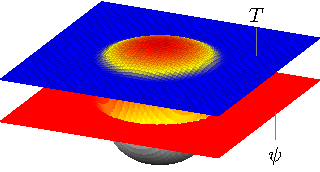
\includegraphics{figures/LinearResponse_bump}
  \caption{Illustration of Luttinger's solution to heat transport. To include a temperature fluctuation $T$, couple the system to some (fictions) gravitational potential $\psi$ giving the same current response as the temperature fluctuation.}
  \label{fig:luttinger-idea}
\end{figure}

A temperature gradient, together with external electric field $\vec{E}$ and chemical potential $\mu$, gives a response in the electrical current $\vec{J}$ and energy current $\vec{J}_E$~\cite{mahanManyparticlePhysics2000}.
One commonly defines the transport coefficient tensors \( L^{ab},\; a,b=1,2 \) containing the response functions such that
\begin{align}
\label{eq:17}
  J_{i} &= -e L^{11}_{ij} \left[
          E_j - T \nabla_j \frac{\mu}{T}
  \right]
  - e L^{12}_{ij} T \nabla_j \frac{1}{T},\\
  J_{E,i} &= L^{21}_{ij} \left[
          E_j - T \nabla_j \frac{\mu}{T}
  \right]
  + L^{22}_{ij} T \nabla_j \frac{1}{T},
\end{align}
with the electric charge \( e = |e| \).
Or, more compactly,
\begin{equation}
  \begin{pmatrix}
    -J_{i} /e \\ J_{E,i }
  \end{pmatrix}
  =
  \vec{L}_{ij}
  \begin{pmatrix}
    E_j - T \nabla_j \frac{\mu}{T}\\
    T \nabla_j \frac{1}{T}
  \end{pmatrix}.
\end{equation}
Importantly, note that these relations are valid when \( \vec{J}, \vec{J}_E \) are understood as the \emph{transport} currents, as opposed to the total currents containing also local non-transporting currents.
This is discussed more with regards to the results of this thesis in \cref{sec:transport-magnetization}.
The coefficients of transportation, $\vec{L}_{ij}$ is a widely used convention, however, several slight variations are used, which at times may cause confusion.
In particular these differences are on which factors of \( T \) and \( \mu \) are included explicitly;
the reason for choosing other definitions might be to have more convenient expressions for the Onsager relation, Seebeck coefficient, thermal conductivity tensor, etc~\cites{mahanManyparticlePhysics2000,chernodubThermalTransportGeometry2021,lundgrenThermoelectricPropertiesWeyl2014}.
The success of Luttinger's method was that the transport coefficients could now be calculated directly, and yielded the same results as had previously been found by less formal approaches.

By the introduction of the Hamiltonian perturbation $H_L$, the response may now be investigated in the Kubo formalism.
By the response in \cref{eq:lin-response-1} the electric current generated from the gravitational perturbation is
% \begin{equation}
%   \braket{\vec{J}^i}(t, \vec{r}) =
% \int \mathrm{d}t' \mathrm{d} \vec{r'} \left\{
%   \frac{-i}{\hbar} \Theta(t-t') \Braket{\left[
% \vec{J}^i(t, \vec{r}), T^{00}(t', \vec{r'})
%     \right]}
% \right\} 
% g_{00}(t', \vec{r'}),
% \end{equation}
\begin{equation}
  \label{eq:current-from-gravity}
  \braket{\vec{J}^i}(t, \vec{r}) =
\int \mathrm{d}t' \mathrm{d} \vec{r'} \left\{
  \frac{-i}{\hbar} \Theta(t-t') \Braket{\left[
\vec{J}^i(t, \vec{r}), T^{00}(t', \vec{r'})
    \right]}
\right\} 
\psi (t', \vec{r'}),
\end{equation}
where the integration is taken over the entire spacetime.
In order to express this as a response to the thermal gradient, we wish to get the gradient of the gravitational potential.
To do this, firstly the $00$-element of the energy-momentum tensor will be expressed in terms derivatives of $T^{j0}$, and then a partial integration will swap the derivative between the energy-momentum tensor and gravitational potential.
Note first that in the flat system the conservation law of the  energy and momentum is simply
\begin{equation}
  \partial _0 T^{00}(t, \vec{r}) + v_F \partial _i T^{i0} (t, \vec{r}) = 0,
\end{equation}
where $v_F$ is the Fermi velocity.
By the fundamental theorem of calculus this obviously gives for the zero-zero component of the energy-momentum tensor
\begin{equation}
  \label{eq:18}
  T^{00}(t, \vec{r}) = - \int\limits_{-\infty }^t \mathrm{d}t'
  v_F \partial _i T^{i 0}(t', \vec{r}).
\end{equation}
Introduce \cref{eq:18} in the response relation \cref{eq:current-from-gravity}, and use integration by parts
\begin{equation}
  \int u v' = uv - \int u' v,
\end{equation}
giving
\begin{equation}\label{eq:current-luttinger-gravity-final}
  \braket{\vec{J}^i}(t, \vec{r}) =
  \int\limits_{-\infty}^{t} \mathrm{d}t'
  \int \mathrm{d} \vec{r'}
  \int\limits_{-\infty }^{t'} \mathrm{d}t''
  \left\{
    \frac{-i v_{F}}{\hbar} \Braket{\left[
        \vec{J}^i(t, \vec{r}), T^{j0}(t'', \vec{r'})
      \right]}
  \right\} 
  \partial'_j \psi (t', \vec{r'}),
\end{equation}
where we have defined \( \partial'_i = \partial /\partial r'_i \).
By Luttinger's relation
\begin{equation}\label{eq:current-luttinger-final}
  \braket{\vec{J}^i}(t, \vec{r}) =
  \int\limits_{-\infty}^t \mathrm{d}t'
  \int \mathrm{d} \vec{r'}
  \int\limits_{-\infty }^{t'} \mathrm{d}t''
  \left\{
    \frac{i v_{F}}{\hbar} \Braket{\left[
        \vec{J}^i(t, \vec{r}), T^{j0}(t'', \vec{r'})
      \right]}
  \right\} 
  \frac{
    \partial'_j T (t', \vec{r'})}{
    T(t', \vec{r'})
  },
\end{equation}
where care must be taken to distinguish the energy-momentum tensor $T^{j0}$ and the temperature $T$, differentiated by the indices, or lack thereof.
\todo{Check the sign here. Depending on how we understand Luttinger's method, it should be positive or negative.}


% \todo{The following section might  be moved. If we want it, need to unify. See park}
% In the interest of expressing  the gravitational potential in terms of the metric tensor, recall that in the Newtonian limit of general relativity, corresponding to $v /c \to 0$, the metric reduces to~\cite{kachelriessQuantumFieldsHubble2018}
% \begin{equation}
%   \mathrm{d}s^2 = \left( 1 + 2\psi  \right) \mathrm{d}t^2 - \left( 1 - 2 \psi  \right) \left( \mathrm{d}x^2 + \mathrm{d}y^2 + \mathrm{d}z^2 \right),
% \end{equation}
% with $\psi $ being the well-known Newtonian gravitational potential.
% Thus, we see that, remembering the definition of the line element $ds = g_{\mu \nu } \mathrm{d}x^{\mu } \mathrm{d}x^{\nu }$,
% \begin{equation}
%   g_{00} = 1 + 2\psi.
% \end{equation}
% One may therefore equivalently to \cref{eq:current-from-gravity} consider the response to variations of the metric component $g_{00}$ giving a term in the Hamiltonian
% \begin{equation}
%   H_L' = \int \mathrm{d}\vec{r}  \frac{g_{00}}{2} T^{00}
% \end{equation}
% with response 
% \begin{equation}
%   \braket{\vec{J}^i}(t, \vec{r}) =
% \int \mathrm{d}t' \mathrm{d} \vec{r'} \left\{
%   \frac{-i}{\hbar} \Theta(t-t') \Braket{\left[
% \vec{J}^i(t, \vec{r}), T^{00}(t', \vec{r'})
%     \right]}
% \right\} 
% \frac{\psi (t', \vec{r'})}{2},
% \end{equation}
% where the two response functions are equal.

% \todo{There is something wrong here. See park et al etc. What happens in the determinant?}


% \setchapterpreamble[or]{%
% \vspace{-1cm}%
% \renewcommand{\dictumwidth}{0.5\textwidth}\renewcommand{\raggeddictum}{\raggedleft}\renewcommand{\raggeddictumauthor}{\raggedleft}%
% % \dictum[Zee]{Not Fermi, nor Teller, nor Wentzel could recall what Feynman had said. All they remembered was his strange notation: p with a funny slash through it.}
% \dictum[Paul Dirac\footnotemark{}]{``I have an equation; do you have one too?''}%
% }

\setchapterpreamble[u]{%
\vspace{-2em}%
\renewcommand{\dictumwidth}{0.5\textwidth}%
\dictum[Paul Dirac\footnotemark{}]{``I have an equation; do
  you have one too?''}%
\vspace{1em}%
}
\chapter{Anomalies in Quantum Field Theory}
\footnotetext{As quoted in~\cite{zeeQuantumFieldTheory2010}.}
%% http://tp.lc.ehu.es/TAE/lectures/lecture4.pdf
% An anomaly is the breaking of a classical symmetry due to quantum corrections.
% More explicitly, we say we have an anomaly when Noether's theorem predicts a conserved current do to a symmetry in the classical action, which is shown to not be conserved when considering quantum corrections to the current.

From Noether's theorem, described in the following section, we know that any continuous symmetry of the Lagrangian $\mathcal{L}$ in a classical consideration will lead to a conserved current.
However, we know from the path integral formulation of \gls{qft} that for a system with fields $\phi $ and an external source $J$, it is the generating functional
\begin{equation}
  \label{eq:generating_functional}
  Z[J] \equiv
  \int \mathcal{D}\phi 
  \exp \left[
  i \left( S[\phi] + \int \mathrm{d}^4x J(x) \phi(x) \right)
  \right] 
\end{equation}
that must be invariant for a transformation to be a symmetry operation of the system.
Quantum corrections from the second quantization can lead to the symmetry group of the generating functional to be smaller than the symmetry group of the classical action, in which case we say there is an \emph{anomaly}.
In that case, the conserved current predicted by Noether's theorem is no longer protected by symmetry, as the operation is indeed not a symmetry of the system.
The terms breaking the classical conservation are called \emph{anomalies}.

It should also be noted that the terminology \emph{anomaly} and \emph{breaks the classical symmetry} are somewhat misleading;
there is no actual symmetry breaking -- in the quantum theory there is no symmetry to begin with, and a more fitting language to describe the situation is that there is an anomalous symmetry in the classical Lagrangian, which is not there in the ``real'' theory.
Thus, the situation must not be confused with spontaneous symmetry breaking, and there is no Goldstone boson present.

\section{Noether's theorem}
The following section is inspired by the derivation of~\citeauthor{kachelriessQuantumFieldsHubble2018}~\cite{kachelriessQuantumFieldsHubble2018}.

Noether's theorem is one of the most central results in theoretical quantum physics.
It relates continuous symmetries with conserved quantities, which for example explain fundamental principles such as conservation of momentum and conservation of energy.
Given a Lagrangian $\mathcal{L}(\phi_a, \partial_{\mu}\phi_a)$ dependent on the fields $\phi_a$, we will consider the variations $\delta\phi_a$ that leave the action, and thus equations of motion, invariant.
That is, the variations that are generators for some continuous symmetry of the system.
Firstly, we will restrict our consideration to the case where the Lagrangian itself is invariant
\begin{equation}
  0 = \delta \mathcal{L} =
  \frac{\delta \mathcal{L}}{\delta \phi_a} \delta\phi_a + \frac{\delta \mathcal{L}}{\delta\partial_{\mu}\phi_a} \delta\partial_{\mu}\phi_a.
\end{equation}
In the last term use that the variation and derivation may be exchanged, $[\delta\partial_{\mu}, \partial_{\delta}\delta] = 0$, and in the first term use the Lagrange equations
\begin{equation}
  \label{eq:lagrange_eq}
  \frac{\delta \mathcal{L}}{\delta\phi_a} = \delta_{\mu} \left( \frac{\delta \mathcal{L}}{\delta \partial_{\mu}\phi_a} \right).
\end{equation}
By the product rule it follows that
\begin{equation}
  \label{eq:noether-1}
  0 = \delta \mathcal{L} =
  \partial_{\mu}\left( \frac{\delta \mathcal{L}}{\delta\partial_{\mu}\phi_a} \right) \delta \phi_a
  + \frac{\delta \mathcal{L}}{\delta\partial_{\mu}\phi_a} \partial_{\mu}\delta \phi_a
  = \partial_{\mu} \left( \frac{\delta \mathcal{L}}{\delta\partial_{\mu}\phi_a} \delta\phi_a \right).
\end{equation}
Thus, we see that the quantity in the parenthesis after the last equality must be conserved.
We denote this quantity $j^{\mu}$, and call it a \emph{current}.

So far, we have the result that for any variation $\delta \phi_a$ that leave the Lagrangian invariant, there is a conserved current
\begin{equation}
  j^{\mu} = \frac{\delta \mathcal{L}}{\delta \partial_{\mu}\phi_a} \delta\phi_a, \quad \partial_{\mu}j^{\mu} = 0.
\end{equation}
There is, however, an even stronger formulation of Noether's theorem.
As the equations of motion are only dependent on the transformation being a symmetry transformation of the action, we realize that even a change in the Lagrangian of the form $\delta \mathcal{L} = \partial_{\mu}K^{\mu}$ will not change the equations of motion, as long as boundary terms of the integral over the Lagrangian may be dropped ($K\to  0, r \to \infty$).
Thus, altering the starting point in Eq. (\ref{eq:noether-1}) to $0 = \delta \mathcal{L} - \partial_{\mu}K^{\mu}$ we get Noether's theorem, theorem \ref{sec:noethers-theorem}.
\begin{theorem}[Noether's theorem]\label{sec:noethers-theorem}
  For any continuous transformation that leave the Lagrangian $\mathcal{L}$ invariant up to a total derivative $\partial _{\mu }K^{\mu }$, there must be an associated conserved current
  \begin{equation}
    \label{eq:noether_thm}
    j^{\mu} = \frac{\delta \mathcal{L}}{\delta \partial_{\mu} \phi_a} \delta \phi_a - K^{\mu}, \quad \partial_{\mu }j^{\mu } =0.
  \end{equation}
\end{theorem}


\section{The axial/chiral anomaly}
%% Note: look at https://www.damtp.cam.ac.uk/user/tong/gaugetheory/3anom.pdf
%% Note: could we include some of the discussion about
%%       Tr([a,adagger]) in https://www.damtp.cam.ac.uk/user/tong/gaugetheory/3anom.pdf
%%       This might be useful when later dealing with fingerprints approach.
We will first give a quick and somewhat superficial introduction to the axial anomaly\footnote{Also known as the chiral anomaly.}, and why it matters in condensed matter physics.
That discussion will be based on the discussion given in~\citeauthor{wehlingDiracMaterials2014}~\cite{wehlingDiracMaterials2014} and~\citeauthor{tongGaugeTheoryLecture}~\cite[Ch.~3]{tongGaugeTheoryLecture}.
Then we will present a more thorough derivation of the anomaly, based on the derivation of~\citeauthor{zeeQuantumFieldTheory2010}~\cite{zeeQuantumFieldTheory2010} and~\citeauthor{kachelriessQuantumFieldsHubble2018}~\cite{kachelriessQuantumFieldsHubble2018}.

In the massless case the Dirac equation reduce to the Weyl equation, whose solutions are right and left moving fermions.
In 1+1 dimensions they have the energy dispersion
\[
  \epsilon  _{\pm} = \pm |p|,
\]
where the $\pm$ indicate positive and negative energy solutions.
Consider the case now in the Dirac sea picture.
The negative energy solutions, antiparticles in high energy physics  and holes in condensed matter physics, are all filled, with the energy band going to $\pm \infty $ momentum.
The particles with energy $\epsilon  = +p$ are right moving solutions, while $\epsilon  = -p$ represent left moving solutions.
Note that in this language, an antiparticle with negative momentum, is right moving, and of course a particle with positive momentum is right moving.
The situation is shown in the left pane of Figure \ref{fig:chiral-dispersion}.
Introduce now an electric field \(E\).
This will cause the states to shift, according to $\dot{p} = e E$, with $e$ being the electric coupling, which is here taken to be the fundamental charge;
note that this shift does not discriminate against left and right movers, they are both shifted the same.
For a field $E > 0$ the right movers are shifted towards higher energies and the left movers are shifted towards lower energies, shown in the right pane of Figure \ref{fig:chiral-dispersion}.
This also shifts the densities of left and right movers!
Denote by $n_+$ the right movers and $n_-$ the left movers.
The total density $n = n_+ + n_-$ is constant, however, the difference $n_+ - n_-$ is not conserved.
Identifying $J = n_+ + n_-$ as the vector current and $J_A = n_+  - n_{-}$ as the axial current, we see that the vector current is conserved, but the \emph{axial} current is not!
Notice how the origin of the anomaly in this context, is the infinite depth of the Dirac sea.

\begin{figure}[th]
  \centering
  % \resizebox{0.4\textwidth}{!}{
    \begin{tikzpicture}
      \begin{axis}[
        cycle list shift=-2,
        width=0.4\textwidth,
        xlabel=\(k\),
        ylabel=\(\epsilon \),
        ytick=\empty,
        xticklabels={,,}, yticklabels={,,},
        extra y tick style = {grid = major },
        extra y tick labels = 0,
        extra y ticks = 0,
        legend columns = 3,
        legend entries = {Filled right movers, Filled left movers},
        legend to name = leg,
        ]
        \addplot [domain=-4:0, samples=10, mark=none, very thick, blue] {x};
        \addplot [domain=0:4, samples=10, mark=none, very thick, red] {-x};
        \addplot[domain=0:4, samples=2, mark=none] {x};
        \addplot[domain=-4:0, samples=2, mark=none] {-x};
      \end{axis}
    \end{tikzpicture}
    % }
  % \resizebox{0.4\textwidth}{!}{
    \begin{tikzpicture}
      \begin{axis}[
        cycle list shift=-2,
        width=0.4\textwidth,
        xlabel=\(k\),
        ylabel=\(\epsilon \),
        ytick=\empty,
        xticklabels={,,}, yticklabels={,,},
        extra y tick style = {grid = major },
        extra y tick labels = 0,
        extra y ticks = 0,
        domain=-4:4,
        ]
        \addplot[samples=2, mark=none] {x};
        \addplot[samples=2, mark=none] {-x};
        \addplot [domain=-4:1, samples=10, mark=none, very thick, blue] {x};
        \addplot [domain=1:4, samples=10, mark=none, very thick, red] {-x};
      \end{axis}
    \end{tikzpicture}\\

    \ref{leg}  % Legend
    % }
    \caption{Dispersion of Weyl fermions, black showing unfilled states, blue filled right movers, and red filled left movers.
      \textbf{(Left)} No electric field applied, Fermi level at the crossing.
      \textbf{(Right)} Electric field in the positive direction applied, shifting the filled states.
      See main text for details.
    \label{fig:chiral-dispersion}}
\end{figure}

\begin{comment}
  % Taken  from wehling
  To put this in the context of condensed matter physics, we will consider the lowest Landau level in a 3D Weyl SM, with the energy $\epsilon = - s\hbar v_F \vec{k} \cdot \hat{B}$, where $s$ is the chirality of the Weyl point and $\hat{B}$ is the direction of the $\vec{B}$-field~\cite{arjonaFingerprintsConformalAnomaly2019}.
  Applying then an electric field $\vec{E}$ perpendicular to the magnetic field $\vec{B}$, all states will be shifted along the electric field according to $\hbar \vec\dot{k} = -e \vec{E}$, with the minus sign coming from the electron having negative charge.
  For the lowest level state, which is chiral, this means that electrons are either disappearing or appearing at the Weyl point.
  The charge is thus not locally conserved around the Weyl point, with the modified continuity equation
  \begin{equation}
    \frac{\partial n}{\partial t} + \nabla \cdot \vec{J} =
    \pm \frac{e^2}{4 \pi^2 \hbar^2 } \vec{E} \cdot \vec{B}.
  \end{equation}
  This non-conservation is an inherently quantum effect.
  Interestingly, this gives yet another explanation, in addition to the Chern conservation explanation, as to why Weyl points must always appear in pairs of opposite chirality, as overall the charge must of course be conserved.
  This gives rise to an interesting effect, which manifests itself in the materials transport properties.
  For a pair of opposite Weyl points separated in momentum space, the anomaly gives an imbalance between the two nodes
  \begin{equation}
    \frac{\partial (n_+ - n_-)}{\partial t} = \frac{e^2}{2 \pi^2 \hbar^2} \vec{E} \cdot \vec{B}.
  \end{equation}
  This charge imbalance, between the nodes separated in momentum space, can be relaxed only by a large momentum scattering, and thus the relaxation time is very long for systems with few impurities.
  This causes the conductivity along the direction of the magnetic field to increase~\cite{wehlingDiracMaterials2014}.
\end{comment}

We will now give a purely field theoretical derivation of the axial anomaly, under a gauge transformation
\begin{equation}
  \psi \to  e^{i \theta + i\theta \gamma^5} \psi,
\end{equation}
corresponding to a gauge transformation of the coupling fields.
\todo{remove or write more about these coupling fields, as we do not have them in our Lagrangian. See Zee and Kachelriess}
As is often the case, there are many ways to do this.
For example, one could show directly that the measure of the path integral is not invariant under a transformation.
We will, however, show it in a somewhat crude way, but where there are no complicated formal considerations, only brute force calculation which is hopefully more readily appreciated by those not familiar to the concept.
The calculation also has some historical importance, as the problem we will solve is in fact exactly the same as the problem that led to the discovery of anomalies!
\todo{Consider to spice up this historic reference}

We will calculate the triangle diagram
% \begin{figure}[h]
  % \centering
\begin{center}
  \feynmandiagram [vertical'=t2 to t3, spring electrical layout]{
    t1[label=left:\(\gamma ^{\lambda }\gamma ^5 \)]
    -- [fermion, edge label=\(p\)] t2 [label=above:\(\gamma ^{\mu }\)]
    -- [fermion, edge label=\(p-k_1\)] t3 [label=below:\(\gamma ^{\nu }\)]
    --  [fermion, edge label=\(p-q\)] t1,
    t2 -- [photon] p1 ,
    t3 -- [photon] p2 ,
    p1 -- [opacity=0] p2, %% Helper line to make photons parallell
  };
\end{center}
% \end{figure}
and show that this leads to the conclusion that either the vector current or the axial current is non-conserved.
The amplitude of the diagram is
\begin{equation}
  \Braket{0|
    T J_5^{\lambda} J^{\mu} J^{\nu}|
  0},
\end{equation}
with the vector current $J^{\mu }= \bar{\psi} \gamma ^{\mu } \psi $ and the axial current $J_5^{\mu } = \bar{\psi} \gamma ^{\mu } \gamma ^5\psi $.
Written out explicitly in momentum space
\begin{multline}
  \label{eq:amplitude}
  \mathcal{A}^{\lambda \mu \nu}(k_1, k_2) =\\
  (-1) i^3 \int \frac{\mathrm{d}^4p}{(2 \pi)^{4}}
  \operatorname{Tr}\left(
    \gamma^{\lambda}\gamma^5 \frac{1}{\slashed{p} - \slashed{q}}
    \gamma^{\nu} \frac{1}{\slashed{p} - \slashed{k}_{1}}
    \gamma ^{\mu} \frac{1}{\slashed{p}}
    % Next term %%%
    +
    \gamma ^{\lambda}\gamma^5 \frac{1}{\slashed{p} - \slashed{q}}
    \gamma ^{\mu } \frac{1}{\slashed{p} -\slashed{k}_{2}}
    \gamma ^{\nu } \frac{1}{\slashed{p}}
  \right),
\end{multline}
where $q = k_1 + k_2$.
For the vector current to be conserved the requirement $k_{1\mu }\mathcal{A} ^{\lambda \mu \nu } = k_{2\nu }\Delta ^{\lambda \mu \nu } = 0$ must hold.
For the axial current to be conserved, the requirement is $q_{\lambda }\mathcal{A}^{\lambda \mu \nu } = 0$.
\todo{show or cite the requirements. I think maybe it is quite simple to see from the wick contractions}

One must be careful when carrying out this calculation, as is also stressed in many textbooks dealing with this issue, for example~\cite{kachelriessQuantumFieldsHubble2018} and~\cite{zeeQuantumFieldTheory2010}.
Consider the criterion for the vector current to be conserved
\begin{equation}
  \label{eq:criterion-conserved}
  k_{1\mu } \mathcal{A} ^{\lambda \mu \nu } (k_1, k_2) =
  i\int \frac{\mathrm{d}^4p}{ (2\pi)^{4}}
  \operatorname{Tr}\left(
    \gamma ^{\lambda } \gamma ^5 \frac{1}{\slashed{p} - \slashed{q}} \gamma ^{\nu}
    \frac{1}{\slashed{p} - \slashed{k}_{1}}
    -
    \gamma ^{\lambda }\gamma ^5 \frac{1}{\slashed{p} -\slashed{k}_{2}} \gamma ^{\nu }\frac{1}{\slashed{p}}
  \right)
  = 0.
\end{equation}
When calculating the integral it might be tempting to simply perform a change of variables, rendering the two terms equal and thus concluding that the criterion  is met.
However, we must notice that the integrand goes like $1 / p^2$ while the boundary surface of a 3-sphere is proportional to $p^3$.
The boundary terms does therefore not vanish, and there is an extra term associated with performing such a change of variables.

Consider that we want to integrate over the function $f$
\begin{equation}
  \int \mathrm{d}^dp f(p).
\end{equation}
If we perform the change of variables $p \to p+a$, one could in theory get an extra contribution from boundary terms, which we will now find.
We will calculate
\begin{equation}
  \int \mathrm{d}^dp \left[ f(p+a) - f(p) \right],
\end{equation}
where we in the first term has ``naively'' performed a change of variables, without considering the boundary terms.
Thus, the result of this integral is indeed the boundary terms.
Firstly, we will perform a Wick rotation into Euclidean space
\todo{some note about why this is allowd, i.e. that there exists some Feynamn parametrization for the}
\begin{equation}
  \int \mathrm{d}^d_Ep \left[ f(p+a) - f(p) \right]
  = \int \mathrm{d}_E^d p \left[ a^{\mu }\partial_{\mu} f(p) + \dots \right].
\end{equation}
Ignoring the higher order terms, the RHS may be rewritten as a surface integral by Gauss's theorem.
Taking the average over the surface integral, and denoting by $S_d(r)$ the surface of a d-sphere with radius r, we write the integral as
\begin{equation}
  \lim_{P\to \infty } a^{\mu } \left( \frac{P_{\mu }}{P} \right) f(P) S_{d-1}(P).
\end{equation}
Rotating back to Minkowski space we gain an additional i, with
\begin{equation}
  \label{eq:shift-trickery}
  \int \mathrm{d}^{d}p \left[ f(p+a) - f(p) \right]
  = \lim_{P\to \infty } ia^{\mu } \left( \frac{P_{\mu }}{P} \right) f(P) S_{d-1}(P).
\end{equation}

We will now perform such a shift of variables in the second term of the trace in Eq.~(\ref{eq:criterion-conserved}), as we notice that shifting $p \to p-k_1$ makes the two terms cancel, leaving only the boundary term.
Let
\begin{equation}
  \label{eq:trace-trickery}
  f(p) = \operatorname{Tr}\left(
  \gamma ^{\lambda }\gamma ^5 \frac{1}{\slashed{p} - \slashed{k}_2} \gamma ^{\nu } \frac{1}{\slashed{p}}
  \right)
  = \frac{\operatorname{Tr}\left(
  \gamma ^5 (\slashed{p}-\slashed{k}_2) \gamma ^{\nu }\slashed{p}\gamma ^{\lambda }
\right)}{
(p-k_2)^2 p^2}
= \frac{{4 i \epsilon ^{\tau \nu \sigma \lambda } k_{2\tau }P_{\sigma }}}{(p-k_2) p^2}.
\end{equation}
Here we used in the first equality the property $1 /\slashed{a} = \slashed{a} /a^2$ twice, and the cyclic permutation invariance of the trace, $\operatorname{Tr}(ABC) = \operatorname{Tr}(BCA)$.
In the second equality, we first wrote the Feynman slash operator by its definition $\slashed{a}=\gamma ^{\mu }a_{\mu }$, and then used the property
\begin{equation}
  \label{eq:trace-gamma}
  \operatorname{Tr}(\gamma ^5\gamma ^{\tau }\gamma ^{\nu }\gamma ^{\sigma }g^{\lambda }) = -4i\epsilon ^{\tau \nu \sigma \lambda },
\end{equation}
where $\epsilon $ is the totally antisymmetric tensor.
The trace can be split into two terms, where the first vanishes as it is proportional to $\epsilon ^{\tau \nu \sigma \lambda }p_{\tau }p_{\sigma }$, and one is left with the expression in Eq. (\ref{eq:trace-trickery}).
Thus, Eq. (\ref{eq:criterion-conserved}) becomes
\begin{equation}
  \label{eq:criterion-conserved-simp}
  k_{1\mu } \mathcal{A}^{\lambda \mu \nu } =
  \frac{i}{(2\pi)^{4}} \lim_{P\to \infty } i(-k_1)^{\mu } \frac{P_{\mu }}{P}
  \frac{{4 i \epsilon ^{\tau \nu \sigma \lambda } k_{2\tau } P_{\sigma }}}{P^{4}} 2\pi^2 P^3
  = \frac{i}{8\pi^2} \epsilon ^{\lambda \nu \tau \sigma } k_{1\tau }k_{2\sigma }.
\end{equation}

Consider now, however, what happens if we shift $p\to p+k_2$ in the first term of Eq.~(\ref{eq:criterion-conserved}) instead.
Surely, if our answer above is correct, any arbitrary shift must yield the same answer.
Similarly to before, let
\begin{multline}
  f(p) = \Tr\left(\gamma^{\lambda }\gamma^5 \frac{1}{\slashed{p} - \slashed{q}} \gamma^{\nu } \frac{1}{\slashed{p} - \slashed{k}_{1}} \right)\\
  = \frac{\Tr \left( \gamma ^5 (\slashed{p}-\slashed{q}) \gamma ^{\nu } (\slashed{p}-\slashed{k}_1)\gamma ^{\lambda } \right)}{
   (p-q)^2(p-k_1)^2
  }
  =
  \frac{-4i\epsilon ^{\tau \nu \sigma \lambda } k_{2\tau } (k_{1\sigma } - p_{\sigma })}{
   (p-q)^2(p-k_1)^2
  },
\end{multline}
where we as above removed all terms symmetric under $\sigma \leftrightarrow \tau$.
Now, Eq. (\ref{eq:criterion-conserved}) becomes
\begin{equation}
  k_{1\mu } \mathcal{A}^{\lambda \mu \nu } =
  \frac{i}{(2\pi)^4} \lim_{P \to \infty } ik_2^{\mu } \frac{P_{\mu }}{P}
  \frac{{-4i\epsilon ^{\tau \nu \sigma \lambda } k_{2\tau } (k_{1\sigma }-p_{\sigma })}}{P^{4}}
  2\pi^2P^3
  = \frac{i}{8\pi^2} \epsilon ^{\lambda \nu \tau \sigma } k_{2\tau }k_{2\sigma }.
\end{equation}
\todo{Check there is not misssing a -1 in last espression}
Where we used that the only term contributing is the $p_{\sigma }$, as the term with $k_{1\sigma }$ goes like $P^{-1}$.
Our results differ depending on the non-physical shift of variables!
As is shown by several textbooks,~\cite{zeeQuantumFieldTheory2010}~\cite{kachelriessQuantumFieldsHubble2018}, this comes from the fact that the integral we started with is in fact linearly divergent -- its value is not well-defined.
What we will have to do, is consider an arbitrary shift $a$ in the integration variable of the amplitude Eq. (\ref{eq:amplitude}), which we will show changes the amplitude by a quantity dependent on $a$.
To cancel this, a counter term must be inserted;
however, as we will see, this counter term can only make either the axial current or the vector current conserved!
Consider now a shift in the integration variable $p \to p - a$ in the amplitude (\ref{eq:amplitude}), where we denote the amplitude with shifted integration variable
\begin{multline}
  \label{eq:amplitude-shift}
  \mathcal{A}^{\lambda \mu \nu}(a, k_1, k_2) =
  (-1) i^3 \int \frac{\mathrm{d}^4p}{(2\pi)^{4}}
  \Tr \left(
    \gamma ^{\lambda } \gamma ^5 \frac{1}{\slashed{p} - \slashed{a} - \slashed{q}} \gamma ^{\nu } \frac{1}{\slashed{p} - \slashed{a}- \slashed{k}_{1}} \gamma ^{\mu } \frac{1}{\slashed{p} - \slashed{a}} \right.\\
    +
   \left. \gamma ^{\lambda }\gamma ^5 \frac{1}{\slashed{p} - \slashed{a}- \slashed{q}} \gamma ^{\mu } \frac{1}{\slashed{p} - \slashed{a} - \slashed{k}_2} \gamma ^{\nu } \frac{1}{\slashed{p} - \slashed{a}}
  \right).
\end{multline}

From Eq. (\ref{eq:shift-trickery}) we already have a formula for the difference
\begin{equation}
  \label{eq:amplitude-difference}
  \mathcal{A}^{\lambda \mu \nu } (a, k_1, k_2) - \mathcal{A}^{\lambda \mu \nu }(k_1, k_2),
\end{equation}
by choosing
\[
  f(p) = \frac{i}{(2\pi)^{4}} \Tr \left( \gamma ^{\lambda }\gamma ^5 \frac{1}{\slashed{p} - \slashed{q}} \gamma ^{\nu } \frac{1}{\slashed{p} - \slashed{k}_{1}} \gamma ^{\mu } \frac{1}{\slashed{p} } \right). 
\]
Ignore for now the prefactor, and note that in the limit
\begin{equation}
  \begin{split}
    \lim_{p\to \infty } f(p) &=
    \frac{\Tr(\gamma ^{\lambda }\gamma ^5 \slashed{p} \gamma ^{\nu } \slashed{p}\gamma ^{\mu }\slashed{p})}{p^6}\\
    &= \frac{2 \Tr(\gamma ^{\lambda }\gamma ^5 \slashed{p}\gamma ^\nu \slashed{p}) - p^2\Tr(\gamma ^{\lambda }\gamma ^5 \slashed{p} \gamma ^{\nu }\gamma ^{\mu })}{p^6}\\
    &= \frac{{4i p_{\sigma }\epsilon ^{\sigma \nu \mu \lambda }}}{p^{4}}.
  \end{split}
\end{equation}
In the second equality we used the anti-commutation relation of gamma matrices in $\slashed{p} \gamma ^{\mu } = 2p^{\mu } - \gamma ^{\mu } \slashed{p}$ and $\slashed{a}^2 = a^2$.
In the last equality, we used again Eq. (\ref{eq:trace-gamma}), and the vanishing of all terms symmetric under interchanging indices when contracted with the fully antisymmetric tensor.
We now find the amplitude difference (\ref{eq:amplitude-difference}).
Firstly, we simplify the  expression slightly as
\begin{equation}
  \Delta \mathcal{A}^{\lambda \mu \nu }(a, k_1, k_2) \equiv \int \mathrm{d}^4p f(p-a) - f(p) +  \{(k_1,\mu ) \leftrightarrow (k_2, \nu )\},
\end{equation}
where the last term indicates to repeat the preceding expression with interchange of $k_1 \leftrightarrow  k_2$ and $\mu \leftrightarrow \nu$.
Thus, by Eq. (\ref{eq:shift-trickery}),
\begin{equation}
  \label{eq:amplitude-difference-explicit}
  \begin{split}
  \Delta \mathcal{A}^{\lambda \mu \nu}(a, k_1, k_2) &=
%  \lim_{p\to \infty } i  a^{\mu } \left( \frac{p_{\mu }}{p} \right) f(p) 2\pi^2p^3
    \lim_{p\to \infty } i  a^{\mu } \left( \frac{p_{\mu }}{p} \right)
  \frac{i}{(2\pi)^{4}} \frac{{4ip_{\sigma }\epsilon ^{\sigma \nu \mu \lambda }}}{p^{4}}
  2\pi^2p^3\\
  &\phantom{=}+ \{(k_1,\mu ) \leftrightarrow (k_2, \nu )\}\\
  &= \lim_{p\to \infty } \frac{{-ia^{\mu }}}{2\pi^2} \frac{{p_{\mu }p_{\sigma }}}{p^2} \epsilon ^{\sigma \nu \mu \lambda } +  \{(k_1,\mu ) \leftrightarrow (k_2, \nu )\}\\
  &= - \frac{ia_{\sigma }}{8 \pi^2}\epsilon ^{\sigma \nu \mu \lambda } +  \{(k_1,\mu ) \leftrightarrow (k_2, \nu )\}.
  \end{split}
\end{equation}
\todo{Figure out if there is missing an overall minus sign}

Now is the time to take a break from the calculations and consider in some detail what this result means, before we will finally carry out the derivation to its end and show the anomaly.
A priori $\mathcal{A}^{\lambda \mu \nu }(a, k_1, k_2)$ should be just as valid as $\mathcal{A}^{\lambda \mu \nu }(k_1,  k_2)$, i.e. setting $a=0$.
In fact, that formulation is quite the misnomer, as $a=0$ is no less arbitrary than any $a\neq 0$ in this setting;
% $p$ is simply a name we have denoted the momentum transfer in our diagram.
$p$ is simply a name by which we denote the moment transfer in our diagram.
\emph{However}, using Eq. (\ref{eq:amplitude-difference-explicit}), leading to
\begin{multline}
  \label{eq:17}
  k_{1\mu } \mathcal{A}^{\lambda \mu \nu }(a, k_1, k_2) - k_{1\mu }\mathcal{A}^{\lambda \mu \nu }(a=0, k_1, k_2) =\\
  -\frac{i}{8\pi^2} \left[
  \epsilon ^{\sigma \nu \mu \lambda } a_{\sigma } +  \{(k_1,\mu ) \leftrightarrow (k_2, \nu )\} \right] k_{1\mu }, 
\end{multline}
we see that the criterion for vector current conservation (\ref{eq:criterion-conserved}) may or may not be met depending on our choice of $a$!
\todo{Should this be related to counter terms as Kachelriess does? What does it really mean that we have to choose some shift}
Owning to a trick from~\citeauthor{zeeQuantumFieldTheory2010}~\cite{zeeQuantumFieldTheory2010}, we will show that the resolve of this is to chose one particular $a$, and the choice will be that $a$ which preserves the consistency of our theory.
Now, this may indeed seem both strange and ad-hoc, how can we justify \emph{choosing} some parameter to get the result we want?
This is, in fact, common in \gls{qft}.
Recall that both the UV-cutoff and dimensional regularization schemes introduce a parameter, which must be determined ``outside'' of our theory.

Let $a=\alpha (k_1+k_2) + \beta (k_1-k_2)$.
This is allowed as $k_1, k_2$ are independent, and the only parameters of our equations.
The $\alpha$ term is obviously symmetric under interchange of $k_1, k_2$, while the $\beta$ term is antisymmetric.
Thus, we see that in Eq. (\ref{eq:17}) only the $\beta $ part survives when adding the pair with interchanged indices and momenta.
Thus,
\begin{align}
  k_{1\mu }\mathcal{A}^{\lambda \mu \nu }(a, k_1, k_2) &=
                                                         -\frac{i}{4\pi^2} \epsilon ^{\sigma \nu \mu \lambda } \beta (k_{1\sigma } - k_{2\sigma })k_{1\mu } + k_{1\mu }\mathcal{A}^{\lambda \mu \nu }(k_1, k_2)\\
                                                       &= \frac{i}{8\pi^2} \left(
                                                         \epsilon ^{\lambda \nu \tau \sigma }k_{1\tau }k_{2\sigma } - 2 \epsilon ^{\sigma \nu \mu \lambda } \beta (k_{1\sigma } - k_{2\sigma })k_{1\mu }\right)\\
  &= \frac{i}{8\pi^2} \epsilon ^{\lambda \nu \tau \sigma } k_{1\tau }k_{2\sigma } (1+ 2\beta ).
\end{align}
Here we inserted our previous result for $k_{1\mu }\mathcal{A}^{\lambda \mu \nu }$ given in Eq. (\ref{eq:criterion-conserved-simp}).
In the last equation we used that $k_{1\sigma }k_{1\mu }$ vanishes when contracted with the Levi Cevita symbol, and relabeled the dummy indices.
It is now  apparent that choosing $\beta = -1 / 2$ makes the criterion for conservation of vector current hold!

By choosing the shift appropriately, the vector current is preserved.
However, it does come at a price.
The requirement for the axial current to be conserved, as mentioned earlier, is
\[
  q_{\lambda } \mathcal{A}^{\lambda  \mu  \nu } = 0.
\]
This amplitude is in fact also set by the parameter $\beta $, as also here $\alpha $ drops out;
we have no free parameter  to tune after fixing $\beta $.
With the choice $\beta  = -1 / 2$, required to conserve the vector current, the axial current will not be conserved!
This is the chiral anomaly.

We could have, of course, instead chosen $\beta $ such that the axial current is conserved, at the expense of the conservation of the vector current.
However, as~\citeauthor{zeeQuantumFieldTheory2010}~\cite{zeeQuantumFieldTheory2010} describes, this would have catastrophic consequences, rendering the entire theory useless.
A non-conserved vector current, would make the fermion number not conserved, clearly non-acceptable.
We therefore chose to sacrifice the axial current instead of the vector current.


\section{The conformal anomaly}
Consider massless \gls{qed}
\begin{equation}
  \mathcal{L} = -\frac{1}{4} F^{\mu\nu}F_{\mu\nu} + i \bar{\psi} \slashed{D} \psi,
\end{equation}
with $\psi$ the Dirac field, $\bar{\psi} = \psi^{\dagger}\gamma^0$, $\slashed{D} = \gamma^{\mu} D_{\mu}$, $D$ the covariant derivative $D_{\mu} = \partial_{\mu}-ieA_{\mu}$, $\gamma^{\mu}$ the Dirac matrices, and $F$ the electromagnetic field.
$A$ is the electromagnetic potential, $\partial _{\mu }A_{\nu } - \partial _{\nu } A_{\mu }$, and $e$ is the coupling, here the fundamental charge.
The theory is classically scale invariant.
That is, under the transformation
\begin{equation}
  x \to \lambda^{-1} x, \quad A_{\mu} \to  \lambda A_{\mu}, \quad \psi \to  \lambda^{\frac{3}{2}}\psi,
\end{equation}
the Lagrangian transforms as
\begin{equation}
  \mathcal{L} \to \lambda^4 \mathcal{L},
\end{equation}
which is canceled by the transformation of measure $\mathrm{d}^4 x \to \mathrm{d}^4x \lambda ^{-4}$ in the action.
As the action is invariant, thus so are the equations of motion.

By Noether's theorem there must be some conserved current corresponding to this symmetry transformation, which we will now show is the dilation current $j_D^{\mu } = T^{\mu \nu } x_{\nu }$.
Consider a conformal transformation of the type $g_{\mu \nu } = e^{2\tau } \eta _{\mu \nu }$, also known as a Weyl transformation of the metric.
The variation of the metric is obviously $\delta g_{\mu \nu } = 2 \tau \eta _{\mu \nu }$.
Recall also that the stress-energy tensor is defined as the response of the action to a variation of the metric
\begin{equation}
  T_{\mu \nu } = \frac{2}{\sqrt{|g|}} \frac{{\delta S}}{\delta  g^{\mu \nu }},
\end{equation}
where $g$ is the determinant of the metric.
Now, using this we see that
\begin{equation}
  \label{eq:diff-action}
  \begin{split}
    \delta  S &= \int \mathrm{d}^4x \frac{\delta S}{\delta g^{\mu \nu }} \delta g^{\mu \nu }\\
    &= \int \mathrm{d}^4x \frac{\sqrt{|g|}}{2 } T_{\mu \nu } \delta g^{\mu \nu }\\
    &= \int \mathrm{d}^4x T_{\mu \nu } \sqrt{|g|} \tau (x) \eta ^{\mu \nu }(x)\\
    &= \int \mathrm{d}^4x \sqrt{|g|} \tau (x) T^{\mu }_{\mu }.
  \end{split}
\end{equation}
As the scaling is a symmetry operation, Eq. \ref{eq:diff-action} must be zero.
As the scaling factor $\tau $ is an arbitrary function, we conclude that the trace $T^{\mu }_{\mu }$ must vanish.
The vanishing trace ensures the conservation of the dilation current as
\begin{align}
  \label{eq:dilation-diff}
  \partial _{\mu } J_D^{\mu } &= T^{\mu \nu }\partial_{\mu } x_\nu +
                                \underbrace{\left( \partial _{\mu }T^{\mu \nu } \right)}_{=0} x_{\nu }\\
  \nonumber &= T^{\mu \nu }\delta _{\mu \nu } = T^{\mu }_{\mu },
\end{align}
where we used the property of the stress-energy tensor that $\partial _{\mu }T^{\mu \nu } = 0$.
As the trace is zero, the dilation current is conserved in the classical picture.

However, this symmetry does not hold when quantum corrections are taken into account.
Loop effects give non-vanishing contributions to the trace, and by Eq.~(\ref{eq:dilation-diff}) this makes the dilation current non-conserved.
Due to this, the conformal anomaly is also often referred to as the trace anomaly.
% Firstly, an intuitive and quick explanation for why the loop effect breaks the symmetry will be given, and then a more lengthy calculation showing this explicitly.
Recall that when calculating the propagators of the \gls{qed} theory, we end up with infinities.
These, we regularize and renormalize, for example with dimensional regularization or UV-cutoff.
In any case, this introduces some dimensionfull scale, $\mu $, the renormalization scale and the cutoff energy respectively for the regulators mentioned.
This scale dependence is encoded in the beta function of the theory, encoding the dependence of the coupling $e$ on the scale,
\begin{equation}
  \beta (e) = \frac{\partial e}{\partial \log \mu };
\end{equation}
if the beta function does not vanish, our theory now has a scale dependence, rendering our theory no longer scale invariant!

% Consider having a derivation of the conformal anomaly here.

When taking into account the loop effects, the trace of the stress-energy tensor is~\cite{kachelriessQuantumFieldsHubble2018}
\begin{equation}
  T_{\mu }^{\mu } = \frac{\beta (e)}{2 e} F_{\mu \nu }F^{\mu \nu },
\end{equation}
where $\beta (e)$ is the beta function of the theory.
This beta function makes the anomaly not exact in one loop, as opposed to the axial anomaly.
In one loop, the massless fermion beta function is~\cite{chernodubAnomalousTransportDue2016}
\begin{equation}
  \label{eq:beta-function}
  \beta ^{(1)} = \frac{e^3}{12 \pi^2}.
\end{equation}

\begin{comment}
  Relating the perturbation $\tau $ to the gravitational potential $\phi $.
  In the Newtonian limit of general relativity, corresponding to $v /c \to 0$, the metric reduces to~\cite{kachelriessQuantumFieldsHubble2018}
  \begin{equation}
    \mathrm{d}s^2 = \left( 1 + 2\Phi  \right) \mathrm{d}t^2 - \left( 1 - 2 \Phi  \right) \left( \mathrm{d}x^2 + \mathrm{d}y^2 + \mathrm{d}z^2 \right),
  \end{equation}
  with $\Phi $ being the well-known Newtonian gravitational potential, coupling to the mass as
  \begin{equation}
    \mathcal{L}_{\text{gravity}} = -\rho \Phi.
  \end{equation}
  \todo{This above is taken simply from my memory. Verify}
  Thus, we see that, remembering the definition of the line element $ds = g_{\mu \nu } \mathrm{d}x^{\mu } \mathrm{d}x^{\nu }$,
  \begin{equation}
    g_{00} = 1 + 2\Phi .
  \end{equation}

  Thus, for a conformal transformation of the metric
  \[
    g_{\mu \nu } = e^{2\tau }\eta _{\mu \nu }, \quad \tau << 1,
  \]
  we identify the Newtonian gravitational potential as $\Phi = 2\tau $
\end{comment}

\begin{comment}
  \section{Notes for the section}
  %% Notes for this section:
  In order to better understand this ... introduce \gls{qft}, Path Integral, Chiral Anomlay
  The renormalization introduces a scale-invariance breaking quantity $\mu$.

  Anomalies must not be confused with spontaneous symmetry breaking, where sym of state is lower than sym of hamiltonian.

  These anomalous currents may give novel transport laws not present in the classical theory.

  There is some word for magnetically reduced/increased conductivity I believe. Magneto-somethingsomething

  The \emph{conformal} scale transformation $g \to g' = e^{2\omega} g$ because lengths are rescaled by a constant factor, while angles are conserved (Kachelriess (17.1))


  Is it not insane that adding the fictitious gravitational potential as we do in Luttinger's approach, can here be treated as an actual metric perturbation!! ???
\end{comment}


% \part{New work}
% \chapter{Charge current from the conformal anomaly}\label{ch:charge-current}
\chapter{Thermoelectric Effect from the Conformal Anomaly}\label{ch:charge-current}
In 2016~\textcite{chernodubAnomalousTransportDue2016} showed that the conformal anomaly of \gls{qed} leads to electrical currents in an inhomogeneous gravitational background.
This effect was further explored by~\textcite{chernodubGenerationNernstCurrent2018}, showing through Luttinger's method that such an anomalous transport could be generated from a temperature gradient, giving additional contributions to the Nernst current.
The same effect was shortly after derived more formally through the Kubo formalism, by \textcite{arjonaFingerprintsConformalAnomaly2019}.

In this chapter we extend the Kubo calculation to tilted Weyl cones.
Firstly, the result for the untilted system is rederived, where we also show several simplifications compared to previous computations.
The results for the untilted cone are then generalized to tilted cones.
The computation is quite lengthy, and the thesis is explicit in each step, with the goal being that a graduate level student should be able to comfortably follow the calculations.

The chapter is divided into sections, each representing a somewhat contained part of the calculation.
The text is not, however, written such that a reader should expect to understand a section without reading the preceeding one.
Due to the nature of the work, certain sections are rather technical.
For the benefit of the reader, we have included summaries of intermediate results, enabling the reader to skip the more technical parts.
In particular, the latter part of \cref{sec:ll-tilt} and section~\ref{sec:explicit-form-tilt} may be skipped without much loss.

We will find the current response of a single Dirac cone, with a temperature gradient $\nabla_y T$ and a magnetic field $B_z$.
The current response of interest in the given geometry is thus in the $x$-direction,
\begin{equation}\label{eq:20}
  J^x = \chi ^{xy} \frac{- \nabla _yT}{T},
\end{equation}
with $\chi^{xy}$  being the response\footnote{The sign in \cref{eq:20} depends on the choice of the response function being the response of the gravitational potential or the temperature gradient. Thus, the sign may differ in the literature.}.
This geometry is shown in \cref{fig:setup}.
\begin{figure}[ht]
  \centering
  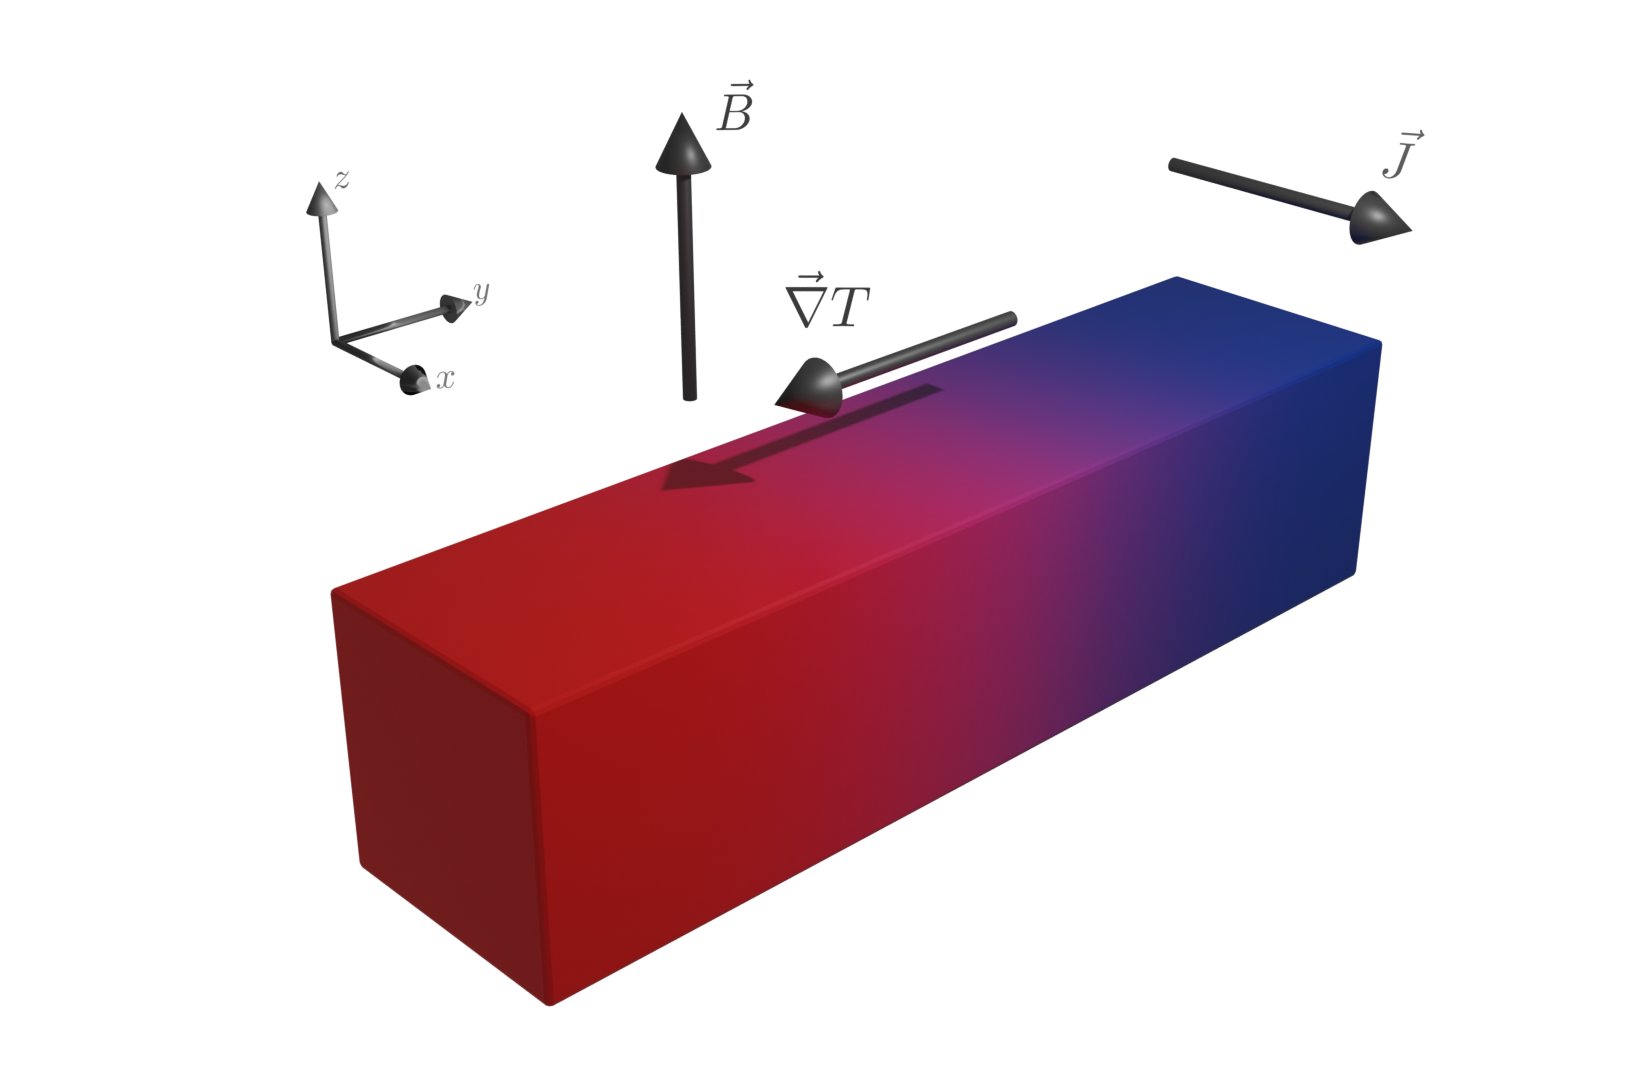
\includegraphics[width=0.7\textwidth]{figures/setup.png}
  \caption{Sketch of the geometry used in the derivation. Note that we consider only bulk response, and the finite sample is only for illustration purposes. \label{fig:setup}}
\end{figure}
In the derivation of~\citeauthor{chernodubGenerationNernstCurrent2018}~\cite{chernodubGenerationNernstCurrent2018} the response
\begin{equation}
  \chi ^{xy} = \frac{e^2 v_F B}{18 \pi ^2 \hbar }
\end{equation}
was found, while the derivation of~\citeauthor{arjonaFingerprintsConformalAnomaly2019}~\cite{arjonaFingerprintsConformalAnomaly2019} found
\footnote{The paper is somewhat unclear on what is their final result, as there is some possible confusion related to the number of Landau levels included and whether one is including both or only one Dirac cone.
The above result is what is meant, to the best of our understanding.}
\begin{equation}
  \chi ^{xy} = \frac{e^2 v_F B}{4 \pi ^2 \hbar }.
\end{equation}

Recall the linear response from the Kubo formalism in \cref{eq:current-luttinger-final}, found through Luttinger's approach.
\begin{equation}
  \label{eq:21}
  \braket{J^i}(t, \vec{r}) = \!\!
  \underbrace{
    \int\limits_{-\infty }^{t} \mathrm{d}t'
    \int \mathrm{d}\vec{r}' \!\!
  \int\limits_{-\infty }^{t'} \mathrm{d}t''
  \left\{
    \frac{-i v_F}{\hbar }
    \Braket{
      [J^i(t, \vec{r}), T^{j 0} (t'', \vec{r}')]
    }
  \right\}
  }_{\chi^{ij}}
  \frac{- \partial _j' T(t', \vec{r}')}{T}.
\end{equation}
Fourier transforming now to the frequency and momentum domain, will be beneficial in our calculations.
As before, the non-perturbed system will be taken to be time and position invariant, such that the correlator in \cref{eq:21} can be taken to depend only on the differences $t-t''$ and $\vec{r} - \vec{r}' $.
Starting with Fourier transforming the position part, notice that the structure of \cref{eq:21} is
\[
  \braket{J^i}(\vec{r}) = \int \mathrm{d} \vec{r}' \chi (\vec{r} - \vec{r}') (-\partial _j' T(\vec{r}') /T),
\]
where the temporal parts were dropped for clarity.
This is a convolution, and the Fourier transform is thus simply given by the product of the two factors~\cite{rottmannMatematiskFormelsamling1995}.
\begin{equation}
  \braket{J^i}(\vec{q}) = -
  \chi (\vec{q}) (iq_j) T(\vec{q}) /T,
\end{equation}
where it was also used that the Fourier transform of a derivative gives the component of the variable.
Showing explicitly how to find the form of the response $\chi $ in momentum space is often overlooked in much literature, and as it does involve some finesse, we want to show it here.
This trick is courtesy of~\citeauthor{changLectureNotesManybody2018}~\cite{changLectureNotesManybody2018}.
By definition, the Fourier transform of the response is, where the variable of integration has been chosen to be $\vec{r}-\vec{r}'$ for later convenience,
\begin{align}
  \chi (\vec{q}) &= \int \mathrm{d}(\vec{r} - \vec{r}') e^{-i\vec{q}(\vec{r}-\vec{r}')} \chi (\vec{r} - \vec{r}')\\
                 &= \int \mathrm{d}(\vec{r} - \vec{r}') e^{-i\vec{q}(\vec{r}-\vec{r}')} C \Braket{
                   \left[
J^i (\vec{r}), T^{j 0}(\vec{r}')
                   \right]},\\
\end{align}
where $C$ denotes $t$-dependent prefactors and integrals over time are omitted, again for clarity of notation.
Note that
\begin{equation}
  \int \mathrm{d}(\vec{r} - \vec{r}') = \frac{1}{\mathcal{V}} \int \mathrm{d}\vec{r} \mathrm{d} \vec{r}',
\end{equation}
where $\mathcal{V}$ is the volume of the system.
Thus,
\begin{equation}
  \begin{split}
    \chi (\vec{q}) &= \frac{1}{\mathcal{V}} \int \mathrm{d}\vec{r} \mathrm{d}\vec{r}'
    e^{-i\vec{q}(\vec{r}-\vec{r}')}
    C \Braket{\left[
        J^i(\vec{r}), T^{j 0}(\vec{r}')
      \right]}\\
    &= \frac{C}{\mathcal{V}} \Braket{\left[ J^i(\vec{q}), T^{j 0}(-\vec{q}) \right]}.
  \end{split}
\end{equation}

Considering now the temporal part, the procedure is simpler.
The linear response still has the form of a convolution, as the response function is only dependent on the difference $t-t'$ by
\todo{Add indices to energy-momentum tensor}
\begin{equation}
  \chi (t-t') = \int\limits_{-\infty }^0 \mathrm{d} t'' \Theta (t - t')
  \Braket{\left[ J^i(t-t'), T^{j0}(t'') \right]},
\end{equation}
where $t''$ was shifted by $t' $, and then the translational invariance of the correlator was used.
In frequency space
\begin{align}
  \chi (\omega ) &= \int \mathrm{d} t e^{i \omega  t} \chi (t)\\
                 &= \int \mathrm{d} t e^{i \omega  t} \int\limits_{-\infty  }^0 \mathrm{d} t''
                   \Theta (t) \Braket{\left[ J^i(t), T^{j 0}(t'') \right]}.
\end{align}
In frequency and momentum space the response function is thus
\begin{equation}\label{eq:22}
  \chi ^{ij} (w, \vec{q}) =
  \frac{-iv_F}{\mathcal{V} \hbar }
  \int \mathrm{d}t e^{i\omega t}
  \int\limits_{-\infty }^{0} \mathrm{d}t'
  \Theta (t)
  \Braket{\left[
      J^i(t, \vec{q}), T^{j 0}(t', -\vec{q})
    \right]}.
\end{equation}

% \section{Complications and considerations}
\section{General remarks}
Before beginning the computation, we here briefly mention some complications and considerations important to our result.
Firstly we discuss how the charge current form a Kubo calculation relate to experimentally measurable currents.
Secondly we discuss the ambiguity related to the energy-momentum tensor.

\subsection{Transport and magnetization}
\label{sec:transport-magnetization}
Recall that we generally define the transport coeffieicents (\cref{eq:17})
\[
J^i = -e L_{ij}^{11} \left[
          E_j - T \nabla_j \frac{\mu}{T}
  \right] - e L^{12}_{ij} T \nabla_j \frac{1}{T},
\]
where \( J^i \) is the electrical current.
In our work, we focus on the \( L^{12} \) coefficient, however the following discussion is valid also more generally.
The definition of transport currents becomes more subtle in systems with broken time-reversal symmetry\cite{vanderwurffMagnetovorticalThermoelectricTransport2019, chernodubThermalTransportGeometry2021}.
In such systems, unobservable, circulating \emph{magnetization} currents arise.
These currents do not contribute to transport, but the Kubo treatment derives the local current, which in general also includes non-transporting currents.
Let
\begin{equation}
  \label{eq:23}
  \vec{J} = \vec{J}_{\text{tr}} + \vec{J}_M,
\end{equation}
where \( \vec{J} \) is the total local current, \( \vec{J}_{\text{tr}} \) is the transport current, and \( \vec{J}_M \) is the circulating magnetization current.
The Kubo formalism generally gives the response to the total local current, \( \chi \);
we are more interested in the experimentally measurable transport response \( L_{ij}^{12} \), related to our Kubo result as
\cite{chernodubThermalTransportGeometry2021}
\begin{equation}
  \label{eq:24}
  L^{12}_{ij} = -\chi_{ij} /e + \epsilon^{ijl} M_l,
\end{equation}
with \( M_l \) the magnetization.
For zero chemical potential, however, these magnetization currents have been shown to go to zero as \( T \to 0 \) \cite{vanderwurffMagnetovorticalThermoelectricTransport2019}.
The result from the Kubo calculation is therefore the actual transport current.


\subsection{Comment on the energy-momentum tensor}\label{sec:commen-T}
There is some ambiguity with regards to the definition of the energy-momentum tensor\cites{kachelriessQuantumFieldsHubble2018}{chernodubThermalTransportGeometry2021}{vanderwurffMagnetovorticalThermoelectricTransport2019}{forgerCurrentsEnergyMomentumTensor2004}.
The \emph{canonical} energy-momentum tensor, derived from Lagrangian mechanics, is defined as
\begin{equation}
	T^{\mu \nu } = \frac{\partial \mathcal{L}}{\partial \partial _{\mu } \psi_i } \partial ^{\nu } \psi_i - \eta^{\mu \nu } \mathcal{L}.
\end{equation}
On the other hand, from general relativity, the \emph{dynamical} energy-momentum tensor is defined by the variation of the (matter) action with respect to the metric\cite{kachelriessQuantumFieldsHubble2018}
\todo{Signs depend on choice of g}
\begin{equation}
	T^{\mu \nu} = \frac{2}{\sqrt{g} } \frac{\delta S}{\delta g_{\mu \nu}}.
\end{equation}
Immediately, we see that the first definition is in general not symmetric, while the latter is, as the metric is always symmetric \footnote{something with torsion never}.
As the energy-momentum tensor is an observable, this presents a problem:
how should the tensor be defined?
This issue is not trivial, and has puzzled physicists for decades\cite{forgerCurrentsEnergyMomentumTensor2004}.

Superficially, we make the following observations.
The \emph{defining} property of the energy-momentum tensor is its conservation law
\begin{equation}
  \label{eq:78}
  \partial_{\mu} T^{\mu \nu} = 0,
\end{equation}
on a flat manifold.
This, of course, only defines the tensor up to a total divergence.
Denote by \( \hat{T}^{\mu \nu} \) the \emph{canonical} energy-momentum tensor.
We can then define another tensor
\begin{equation}
  \label{eq:79}
  T^{\mu\nu} = \hat{T}^{\mu \nu} + \partial_{\alpha} S^{\alpha \mu \nu}.
\end{equation}
By letting the additional term be anti-symmetric \( S^{\alpha \mu \nu} = - S^{\mu \alpha \nu}\), it is divergence free.
This is easily shown as follows:
\begin{align}
  \label{eq:80}
  \partial_{\mu} \partial_{\alpha} S^{\alpha \mu \nu} &= - \partial_{\mu} \partial_{\alpha} S^{\mu \alpha \nu}\\
                                                        &= - \partial_{\alpha} \partial_{\mu} S^{\mu \alpha \nu}\\
  &= -\partial_{\mu} \partial_{\alpha} S^{\alpha \mu \nu},
\end{align}
where we used the commutation of partial derivatives and relabelling of the dummy indices \( \mu, \lambda \).
By an appropriate choice of \( S^{\alpha \mu \nu} \) the canonical energy-momentum tensor may be symmetrized, importantly while still abiding the conservation law.
The correction that symmetrizes the energy-momentum tensor is known as the ``Belifnante tensor'', which for the Dirac Lagrangian is\cite{chernodubThermalTransportGeometry2021}
\begin{equation}
  \label{eq:81}
  S^{\alpha \mu \nu} = \frac{1}{8} \bar{\Psi}\left[ \gamma^{\alpha}, \sigma^{\mu\nu} \right] \Psi,
\end{equation}
which gives
\begin{equation}
  \label{eq:82}
  T^{\mu \nu} = \frac{1}{4} \bar{\Psi} (\gamma^{\mu} D^{\nu} + \gamma^{\nu} D^{\mu}) \Psi.
\end{equation}
Which, in the case of the Dirac Lagrangian, so happens to correspond to the naive symmetrization
\begin{equation}
  \label{eq:83}
  T^{\mu\nu}_s = \frac{T^{\mu \nu} + T^{\nu \mu}}{2}.
\end{equation}

It is also instructive for our work to consider a more naive line of reasoning.
The energy-momentum tensor is used in this work through its conservation law \cref{eq:78}, whose first component gives the conservation of energy.
Writing it out explicitly
\begin{equation}
  \label{eq:84}
  \partial_0T^{00} + \partial_i T^{i0} = \partial_0 \epsilon + \partial_i j^i_{\epsilon} = 0,
\end{equation}
with \( \epsilon \) the energy density and \( \vec{j}_{\epsilon} \) the energy density current, the question is really seen to be finding the energy density current, ignoring all formal arguments about the energy-momentum tensor in a general context.
Using such a line of reasoning \textcite{vanderwurffMagnetovorticalThermoelectricTransport2019} argued that the appropriate form of the energy-momentum tensor that should be used in linear response calculations of Dirac material systems, is the unsymmetrized canonical tensor.
In this work, we will therefore use the canonical energy-momentum tensor, as opposed to the symmetric form used in the linear response calculation of an untitled cone done by \textcite{arjonaFingerprintsConformalAnomaly2019}.
In the untilted case, the two definitions give the same contribution, while for a titled cone, the response from the two definitions differ.

In the case of an untilted system, the components of interest of the canonical energy-momentum tensor reads
\begin{subequations}
\begin{align}
  T^{y 0} &= \frac{s i}{4}
  \left[
  \phi^{\dagger} \sigma_y \partial_{0} \phi - \partial_0 \phi^{\dagger} \sigma_y \phi
  \right],\\
  T^{0 y} &= \frac{v_F}{4}
  \left[
  \phi^{\dagger} p_y \phi - p_y \phi^{\dagger} \phi
  \right].
\end{align}
\end{subequations}
The symmetrized energy-momentum tensor used by \textcite{arjonaFingerprintsConformalAnomaly2019}
\begin{equation}
  T_s^{y 0} = \frac{T^{y 0} + T^{0 y}}{2}.
\end{equation}
The response was found to be
\begin{equation}
  \chi = [\dots] \sum\limits_{\underset{N=M-1}{m,n}}^{} \int \mathrm{d} \kappa_z (F^{(1)} + F^{(2)}) \alpha_{\kappa_z m s}^2,
\end{equation}
with \( [\dots] \) prefactors not relevant here, and \( F^{(i)},\, i=1,2 \) the contribution from \( T^{y0} \) and \( T^{y 0} \), respectively.
They are
\begin{align}
  F^{(1)} &= \epsilon_{\kappa_z m s} + \epsilon_{\kappa_z n s},\\
  F^{(2)} &= s \alpha_{\kappa_z n s} \sqrt{M-1} + \frac{s \sqrt{M}}{\alpha_{\kappa_z m s}},
\end{align}
where we have used the dimensionless
\[
  \epsilon_{\kappa_z m s} = \frac{\sqrt{2eB}}{v_{F}} E_{k_z m s}, \quad \kappa_z = \sqrt{2 e B} k_z.
\]
Using the explicit form of the normalization factor
\[
  \alpha_{k_z m s} = - \frac{s \sqrt{M}}{\epsilon_{m} - s \kappa_z},
\]
and energy eigenstates
\[
  \epsilon_m = \sign (m) \sqrt{M + \kappa_{z}^2},
\]
it is not difficult to show that
\begin{equation}
  F^{(2)} = \epsilon_{\kappa_z m s} + \epsilon_{\kappa_z n s} = F^{(1)}.
\end{equation}

Tilting parallel to the magnetic field does not alter the eigenstates, it only changes the eigenvalues by a factor \( t_{\parallel} v_F k_z \) \cites{yuPredictedUnusualMagnetoresponse2016,tchoumakovMagneticFieldInducedRelativisticProperties2016}, as we will show later.
The results from the untilted case may thus be applied directly, with rescaled energies.
As the normalization factor \( \alpha_{\kappa_z m s} \) is invariant under the tilt, \( F^{(2)} \) does not change.
However, \( F^{(1)} \) changes to
\begin{equation}
  \label{eq:163}
  F^{(1)} = \epsilon_{\kappa_z m s} + \epsilon_{\kappa_z n s} = \epsilon^0_{\kappa_z m s} + \epsilon^0_{\kappa_z n s} + 2 \kappa_z t_{\parallel},
\end{equation}
where \( \epsilon^0_{\kappa_z m s} \) is the energy levels of the untilted system.
The last term in \cref{163} gives a non-zero contribution to the total response, and so the results for a tilted cone is generally dependent on the choice of the energy-momentum tensor.

The calculation presented in the thesis has for completeness been carried out also for the symmetric energy-momentum tensor as well.
The result presented in \cref{sec:otherterm-appendix}.


\todo{Decide dimless or dimfull quantities}

\section{Eigenvalue problem of the Landau levels of a Weyl Hamiltonian}
To evaluate the correlator of the response function, the matrix elements of the current and stress-energy tensor must be found.
In order to do this, we find eigenstates in the Landau basis of the system.
We will first consider the untilted Hamiltonian, which we will then use to find the Landau levels of the tilted Hamiltonian.

\subsection{The untilted Hamiltonian}
\label{sec:ll-notilt}
Couple the Weyl Hamiltonian to the magnetic field through minimal coupling
\begin{equation}
  \label{eq:weyl-hamil}
  H_s = s v_F \sigma^i \left( p_i + e A_i \right),
\end{equation}
with $s$ being the chirality, $p_i$ the momentum operator, and $e = |e|$ the coupling constant to the electromagnetic field $\vec{A}$.
Choose coordinates such that $\vec{B} = B_z \hat{\vec{z}}$, which in the Landau gauge gives $\vec{A} = -B_{z}y \: \hat{\vec{x}}$.
As the Hamiltonian is invariant in $x$ and $z$, take the plane wave ansatz $\phi(\vec{r}) = e^{ik_x x + i k_z z} \phi (y)$.
It then follows
\begin{equation}
  H_s \phi(\vec{r}) = E \phi(\vec{r}) \implies \tilde{H}_s \phi(y)  = E \phi(y),
\end{equation}
where $\tilde{H}$ is the result of replacing $p_z \to  k_z, p_x\to   k_x$ in $H_s$, as the plane wave part of $\phi $ have these eigenvalues.
Absorb the chirality $s$ as a sign in the velocity $v_F$, for more concise notation.
Thus, writing everything explicitly, the spectrum is given by
\begin{equation}
  \label{eq:25}
  -  v_F
  \begin{pmatrix}
    - k_z & \partial _y + e y B_{z} /   - k_x\\
    -\partial _y + e y B_{z} /  -k_x & k_z
  \end{pmatrix}
  \phi(y)  = E\phi(y).
\end{equation}
We will now find the spectrum $E$ of the Hamiltonian.

Inspired by the derivation for the spectrum of the 2D Dirac Hamiltonian in~\cite{wehlingDiracMaterials2014}, we introduce the length scale $l_B = 1 /\sqrt{eB}$, and the dimensionless quantity $\chi = y /l_{B} - k_x l_{B}$.
In dimensionless quantities Eq.~(\ref{eq:25}) is
\begin{equation}
  -\frac{{ v_F}}{l_{B}}
  \begin{pmatrix}
    -k_z l_B & \partial _{\chi } + \chi \\
    -\partial _{\chi } + \chi & k_z l_B
  \end{pmatrix}
  \phi(y)  =  E \phi(y).
\end{equation}
Let the operators \(a = \left( \chi + \partial _{\chi } \right) / \sqrt{2},\; a^{\dagger} = \left( \chi - \partial _{\chi } \right) /\sqrt{2}\).
One may easily verify the commutation relation $[a, a^{\dagger}] = 1$;
they are ladder operators of the harmonic oscillators, whose eigenstates are $\ket{n}$, with $a\ket{n} = \sqrt{n}\ket{n-1}, a^{\dagger} \ket{n} = \sqrt{n+1} \ket{n+1}$.
In terms of these operators, the system is
\begin{equation}
  -\frac{\sqrt{2}  v_F}{l_B}
  \begin{pmatrix}
    -\frac{k_zl_B}{\sqrt{2}} & a\\
    a^{\dagger} & \frac{k_zl_B}{\sqrt{2}}
  \end{pmatrix}
  \ket{\phi } = E \ket{\phi }.
\end{equation}
Take the ansatz
\begin{equation}
  \ket{\phi } =
  \begin{pmatrix}
    \beta \ket{n-1}\\
    \alpha  \ket{n}
  \end{pmatrix},
\end{equation}
which is the most general form of $\ket{\phi }$ with any hope of being an eigenstate.
This leads to
\begin{equation}
  -\frac{\sqrt{2}  v_F}{l_B}
  \begin{pmatrix}
    \left( -\gamma \beta + \alpha \sqrt{n} \right) \ket{n-1}\\
    \left( \beta \sqrt{n} + \gamma \alpha \right) \ket{n}
  \end{pmatrix}
  = E \ket{\phi },
\end{equation}
with $\gamma  = k_zl_B / \sqrt{2}$.
For $n > 0$ this leads to the equation for $\phi $ to be an eigenfunction
\begin{equation}
  -\gamma + \frac{\alpha}{\beta } \sqrt{n} = \frac{\beta }{\alpha } \sqrt{n} + \gamma.
\end{equation}
Solving for $\alpha /\beta $ this gives
\begin{equation}
  \frac{\alpha}{\beta } = \frac{\gamma}{\sqrt{n}} \pm \sqrt{1 + \frac{\gamma^2}{n}},
\end{equation}
and thus
\begin{equation}
  E = \pm v_F \sqrt{
    \frac{2n}{l_B^2} + k_z^2
  }
  = \pm s v_F \sqrt{
    2n e B  + k_z^2
  },
\end{equation}
where we reintroduced the explicit $s$.
For $n = 0$ the annihilation operator $a$ destroys the vacuum state $\ket{0}$, and the energy is instead $E_0 = - s k_z v_F$.
The excited energy states are doubly degenerate;
we choose to denote the energy levels by $m \in \mathbb{Z}$, where the sign from $\pm s$ is taken care of by the sign of this quantum number, and the harmonic oscillator levels $n$ are given by its absolute value $|m|$.
The energy levels are
\begin{subequations}
  \label{eq:26}
  \begin{align}
    \label{eq:27}
    E_{k_z m s} &= \operatorname{sign}(m) v_F \sqrt{2 |m| e B   + k_z^2 } & \text{ for } m \neq 0,\\
    \label{eq:28}
    E_{k_z 0 s} &= -s  k_z v_F & \text{ for } m = 0.
  \end{align}
\end{subequations}
We now find the corresponding eigenvectors of the system.
The solution to the one dimensional harmonic oscillator in position space is, in dimensionless coordinates $\xi$,~\cite[Eq.~18.39.5]{NIST:DLMF}
\begin{equation}
  \braket{\xi | n} = \phi _n (\xi)
  = \frac{1}{\sqrt{2^nn!}} \pi^{-\frac{1}{4}}
  e^{- \frac{\xi^2}{2}} H_n \left( \xi \right),
  % = \frac{1}{\sqrt{2^nn!}} \left( m\frac{\omega}{\pi  } \right)^{\frac{1}{4}}
  % e^{- \frac{{m\omega x^2}}{2 }} H_n \left( \sqrt{\frac{m\omega }{ } x} \right),
\end{equation}
where $H_n$ are the Hermite polynomials.
Thus,
\begin{equation}
  \braket{\chi | \phi } =
  \begin{pmatrix}
    \beta \braket{\chi | n-1}\\
    \alpha \braket{\chi | n}
  \end{pmatrix}
  =
  e^{- \frac{\chi^2}{2}}
  \begin{pmatrix}
    \frac{\beta }{\sqrt{2^{n-1}(n-1)!\sqrt{\pi }}} H_{n-1} \left( \chi \right)\\
    \frac{\alpha }{\sqrt{2^{n}n!\sqrt{\pi }}} H_n \left(\chi \right)\\
  \end{pmatrix},
\end{equation}
where we defined \( H_{-1} = 0 \) in order to get a more general expression.
Choosing
\begin{equation}
  \alpha  = \sqrt{\frac{\gamma^2}{n}} \implies \beta = \frac{1}{1 \pm \sqrt{1 + \frac{n}{\gamma ^2}}} = \pm \frac{\gamma ^2}{n} \left( \sqrt{1 + \frac{n}{\gamma ^2}} - 1 \right),
\end{equation}
gives
\begin{equation}
  \phi (\chi ) = e^{-\frac{\chi^2}{2}} \sqrt{\frac{\gamma ^2}{n}}
  \begin{pmatrix}
    \frac{
      \pm \sqrt{\frac{\gamma ^2}{n}} \left( \sqrt{1 + \frac{n}{\gamma ^2}} - 1 \right)
    }{
      \sqrt{2^{n-1} (n-1)! \sqrt{\pi }}
    }
    H_{n-1}(\chi )\\
    \frac{1}{\sqrt{2^{n}n!\sqrt{\pi }}} H_n \left(\chi \right)
  \end{pmatrix}.
\end{equation}
There are thus four quantum numbers related to the eigenvectors, $k_x,  k_z, m, s$.
Reintroducing $\chi = (y-k_xl_B^2) /l_B$ and normalizing we get:
\begin{summary}
  The Landau levels of a Weyl cone coupled to a magnetic field \( B_z \) has the eigenvalues
  \begin{subequations}
    \begin{align}
      E_{k_z m s} &= \sign(m) v_F \sqrt{2 e B M + k_{z} ^2} &\text{for } m \neq 0,\\
      E_{k_z 0 s} &= - sk_z v_F &\text{for } m = 0.
    \end{align}
  \end{subequations}
  The eigenstates are
  \begin{multline}
    \phi _{\vec{k} m s}(\vec{r}) =
    \frac{1}{\sqrt{L_xL_z}}
    \frac{e^{ik_x x}e^{ik_z z}}{\sqrt{\alpha_{k_z m s}^2 + 1}}
    e^{-\frac{\left(y-k_x l_B^2\right)^2}{2 l_B^2}}\\
    % \frac{
    %   \exp \left[ik_x x + ik_z z - \frac{(y - k_x l_B^2)^2}{2 l_{B}^2}\right]
    % }{
    %   \sqrt{L_{x}  L_z} \sqrt{\alpha_{k_{z} m s}^2 + 1}
    % }
    \times
    \begin{pmatrix}
      \frac{\alpha_{k_z m s}}{\sqrt{2^{M-1} (M-1)! \sqrt{\pi } l_B}} H_{M-1}\left( \frac{y-k_x l_B^2}{l_B} \right)\\
      \frac{1}{\sqrt{2^M M! \sqrt{\pi } l_B}} H_M \left( \frac{y-k_x l_B^2}{l_B} \right)
    \end{pmatrix},
  \end{multline}
  where \( \vec{k} = (k_x, k_z)\), and with the normalization factor
  \begin{equation}
    \alpha_{k_z m s} = \frac{-s \sqrt{2eB M}}{\frac{E_{k_z m s}}{v_{F}} - s k_z}.
  \end{equation}
  Here, capital letters indicate absolute value of corresponding quantity, \( M=|m| \), a convention we will use throughout the chapter.
\end{summary}
\subsection{The tilted Hamiltonian}
As we have seen, the eigenvalues of a Type-II Weyl semimetal are simple to find, and are not qualitatively different from those of Type-I, other than the appearance of particle and hole pockets at the Fermi level.
We will also consider the Landau levels of these materials, which importantly are very different from Type-I.
In fact, erroneous treatment of the Landau spectrum of Type-II semimetals caused the original paper describing Type-II materials to mistakenly assert that the chiral anomaly would not be present for certain directions of a background magnetic field \cites{soluyanovTypeIIWeylSemimetals2015,sharmaChiralAnomalyLongitudinal2017}.

The issue with the Landau level description is that for certain directions of the \(B\)-field, the Landau levels break down.
For Type-I materials, the description is valid for all directions of the \(B\)-field, but as the cone tilts into a Type-II material, the description breaks down when the \(B\)-field and tilt direction are perpendicular \cite{sharmaChiralAnomalyLongitudinal2017}, and as the magnitude of the tilt increases, the Landau levels are only valid up to a certain angle between the tilt direction and magnetic field.
We will in this section derive and elucidate the Landau levels and their regions of validity.

Consider again the Hamiltonian
\begin{equation}
  \label{eq:29}
  H = v_{F} \vec{t}^s  \vec{p} + s v_{F} \vec{p} \vec{\sigma},
\end{equation}
with the \emph{tilt vector} as defined in Eq.~\eqref{eq:11}
\[
  \vec{t}^s
  =
  \begin{cases}
    \vec{t} & \text{ broken inversion symmetry},\\
    s \vec{t} & \text{ inversion symmetry}.
  \end{cases}
\]
To find the Landau levels in a magnetic field \(\vec{B} = B_{z}\hat{z} \), we will ``Lorentz boost'' the system to a frame where the cone is not tilted, where we may use the usual approach for finding the Landau levels.

\todo{Make sure this is not a repetition}
Generally, consider \( \vec{t} \) to  consist of two components: \( \vec{t}_{\parallel} \) which is parallel to the magnetic field, and \( \vec{t}_{\perp} \) perpendicular to the magnetic field.
Without loss of generality, we take the magnetic field to be in the \( z \)-direction, with the Landau gauge \( \vec{A} = - B_z y \hat{x} \).
By a rotation around \( z \), we may also in general take \( \vec{t}_{\perp} \parallel \hat{x} \).~%
\footnote{
  The setup considered in the response calculation does not have \( U(1) \) symmetry around the \( \vec{B} \)-field, due to the temperature gradient \( \nabla T \).
  However, the Landau levels are here computed generally, and when later introducing the symmetry breaking components like the temperature gradient, we simply rotate to an appropriate frame.
}
Thus, let \( \vec{t} = (t_{\perp}, 0, t_{\parallel}) \), and introduce the magnetic field through the minimal coupling \( \vec{p} \to \vec{p}^B = \vec{p} + e \vec{A} \).

The Landau level equation is
\begin{equation}
  \label{eq:30}
  \left(H_{B} - E\right) \ket{\psi } = 0,
\end{equation}
with
\begin{equation}
  \label{eq:31}
  H_{B} = v_F \left(t^s _{\perp} p^B_{x} + t^s _{\parallel} p^B_{z} \right) \mathcal{I}_2 + \sum_i s v_{F} p^B_{i} \sigma _{i},
\end{equation}
where \(\mathcal{I}_{2}\) is the identity matrix of size 2.
We may again make the plane wave ansatz \( \phi(\vec{r}) = e^{i k_x x + i k_z z} \phi(y) \), similar to what was done for the untilted Hamiltonian in section \ref{sec:ll-notilt}, to replace \( p_{(x /z)} \to k_{(x /z)} \).
In order to use the ladder operator method used for the untilted cone, we must get rid of the \(k^B_{x}\) on the diagonal of the Hamiltonian, as we must reformulate the equation in terms of the ladder operators.
\footnote{It would also be possible to choose the frame such that the tilt was both in \(x\) and \(y\) direction, in which case we would get ladder operators also on the diagonal.
  This system, albeight tedious, could also have been solved directly.
  \todo{Verify this}
}
To achieve this, we will use a ``Lorentz boost'', which as we will show only leave \(k_{z}\) and \(E\) in the diagonal.
Act with the hyperbolic rotation operator \(R = \exp[\Theta /2 \sigma_{x}]\) on Eq. \eqref{eq:30} from the left, and insert identity on the form \( R R^{-1} \) before the state vector.
By introducing the state in the rotated frame \(\ket{\tilde{\psi}} = R^{-1} \mathcal{N} \ket{\psi } \), with \(\mathcal{N}\) a normalization factor compensating for the non-unitarity of the transformation, we get the eigenvalue equation
\begin{equation}
  \label{eq:32}
  % (\exp[\Theta /2 \sigma_{x}] H_{B}\exp[\Theta /2 \sigma_{x}] - E \exp[\Theta \sigma_{x}]) \ket{\tilde{\psi}} = 0.
  (R H_{B} R - E R^2) \ket{\tilde{\psi}} = 0.
\end{equation}

We now make the fortunate observation that the diagonal elements of
\[
  R \sigma_{i} R
\]
are zero for $i=y$ and non-zero for \(i=x,z\).
We may thus rotate the \(x\)- and \(z\)-components in and out of the diagonal elements, without accidentaly rotating the \(y\)-components into the diagonal.

We will now find the boost parameter that eliminates \(k_{x}\) from the diagonal.
Note that
\begin{equation}
  \label{eq:33}
  R^{2} = e^{\Theta \sigma _{x} } =
  \begin{pmatrix}
    \cosh \theta & \sinh \theta \\
    \sinh \theta & \cosh \theta
  \end{pmatrix}
\end{equation}
and as $[R, \sigma_{x}] = 0$,
\begin{equation}
  \label{eq:34}
  R \sigma _{x} R =  R^{2} \sigma _{x} =
  \begin{pmatrix}
    \sinh \theta & \cosh \theta \\
    \cosh \theta & \sinh \theta
  \end{pmatrix},
\end{equation}
as the effect of \(\sigma _{x}\) is to transpose the rows.
The problematic part of the Hamiltonian with regards to finding the Landau levels, are the terms containing \(k^B_{x}\) on the diagonal, i.e.
\[
  v_F t^s_{\perp} k^B_{x} \mathcal{I}_{2} + s v_{F} k^B_{x} \sigma _{x}.
\]
The requirement for \(k^B_{x}\) to be rotated out of the diagonal is thus
\begin{equation}
  \label{eq:35}
  t^s_{\perp} \cosh \theta + s \sinh \theta = 0.
\end{equation}
Solving for \(\theta \) we get
\begin{equation}
  \label{eq:36}
  \theta = \log (
  \pm \frac{\sqrt{s - t^s_{\perp}}}{\sqrt{s + t^s_{\perp}}}
  ).
\end{equation}
Alternatively, written in a slightly suggestive form,
\begin{equation}
  \label{eq:37}
  \tanh \theta =
  - s t^s_{\perp},
\end{equation}
which is of course on the form of the \emph{rapiditiy} known from Lorentz transformations, with \( -s t^{s}_{\perp} \) taking the place of the \( \beta = v / c \) factor.
From this observation, we also find it instructive to introduce the Lorentz factor
\begin{equation}
  \label{eq:gamma-lorentz}
  \gamma = \frac{1}{\sqrt{1 - \beta^2} } = \frac{1}{\sqrt{ 1 - t_{\perp}^2 }}.
\end{equation}

The required hyperbolic tilt angle to eliminate the \(k^B_{x}\) in the diagonal elements of the Hamiltonian, originating from the tilt, is thus
\begin{equation}
  \label{eq:38}
  \theta = - s \tanh^{-1} t^s_{\perp}.
\end{equation}
The inverse of \(\tan \), of course, diverges as the argument approaches \(\pm 1\), as shown in Figure \ref{fig:arctanh}.
\begin{figure}[ht]
  \tikzsetnextfilename{arctanh}
  \centering
  \begin{tikzpicture}
    \pgfkeys{/pgf/declare function={arctanh(\x) = 0.5*(ln((1+\x)/(1-\x)));}}
    \begin{axis}[
      xmin=-1.2, xmax=1.2,
      ymin=-3.9, ymax=3.9,
      samples=200,
      enlarge x limits=false,
      grid=both,
      no markers,
      % axis equal
      xlabel=\(x\),
      ylabel=\(\tanh^{-1} x\),
      % ytick=none,
      ]
      \addplot +[thick,domain=-0.999:0.999] {arctanh(x)};
      \draw [thick,dashed,domain=-0.99:0.99] (1,-4) -- (1,4);
      \draw [thick,dashed,domain=-0.99:0.99] (-1,-4) -- (-1,4);
    \end{axis}
  \end{tikzpicture}
  \caption{\label{fig:arctanh} Plot of \(\tanh^{-1}\), which diverges as the argument goes to \(\pm 1\).}
\end{figure}
For \(|t_{\perp}| < 1\) we are able to find an angle \(\theta \) which transforms our Hamiltonian into a form which we may solve.
For \(|t_{\perp}| \geq 1\), however, no (real) solution of \(\theta \) exits, and the Landau level description collapses.
More concretely, as we will show later, the separation of the landau levels is reduced as the perpendicular tilt increases, and as \( |t_\perp| \to 1 \), the level separation \( \Delta E \to 0 \).

Interestingly, there are no restrictions in the perpendicual tilt, \( t_\parallel \).
The \( \vec{t} \) parametrization of the tilt is conveniently visualized by plotting the \( t \)-vector inside a unit sphere, shown in Figure \ref{fig:tiltSphere}.
If the vector is outside the unit sphere, it is a Type-II, if it is inside, it is a Type-I.
Also, if the projection of the vector onto the \(x,y\)-plane is on the unit disk, the Landau level description is valid, if not, the Landau levels collapse.
When the projection is on the unit disc, the system is in the \emph{magnetic} regime, otherwise we denote it by the \emph{electric} regime.
All Type-I materials may thus be described by Landau levels, while it for Type-II is only valid for certain directions of \(\vec{t}\).
As the \(t\)-vector gets larger, the magnetic regime is restricted to smaller angles between \( \vec{t} \) and \( \vec{B} \).
\begin{figure}[ht]
  \centering
  % 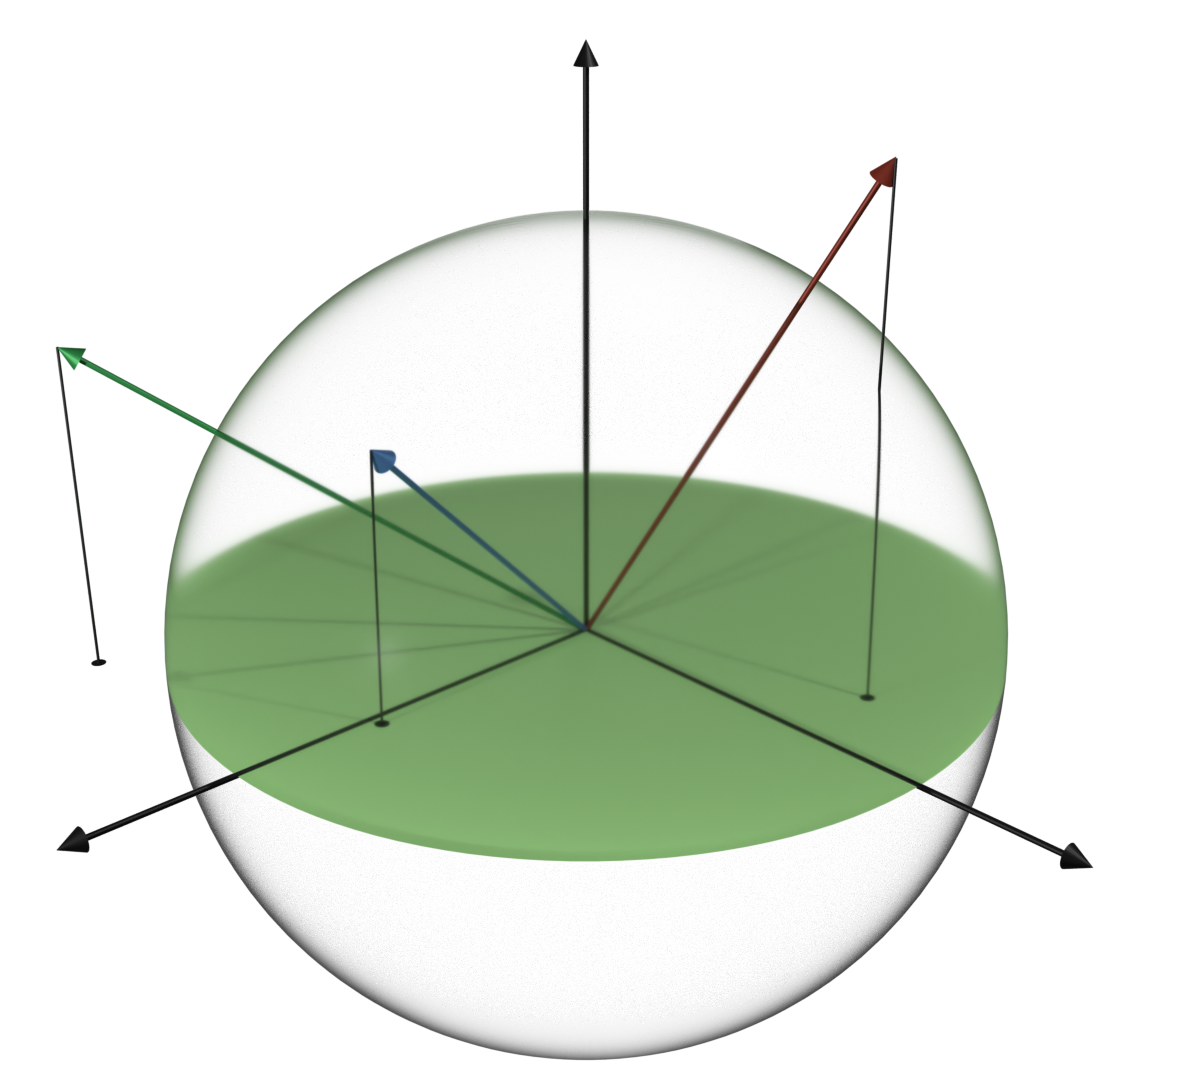
\includegraphics[width=0.75\textwidth]{figures/tiltSphere.png}
  % 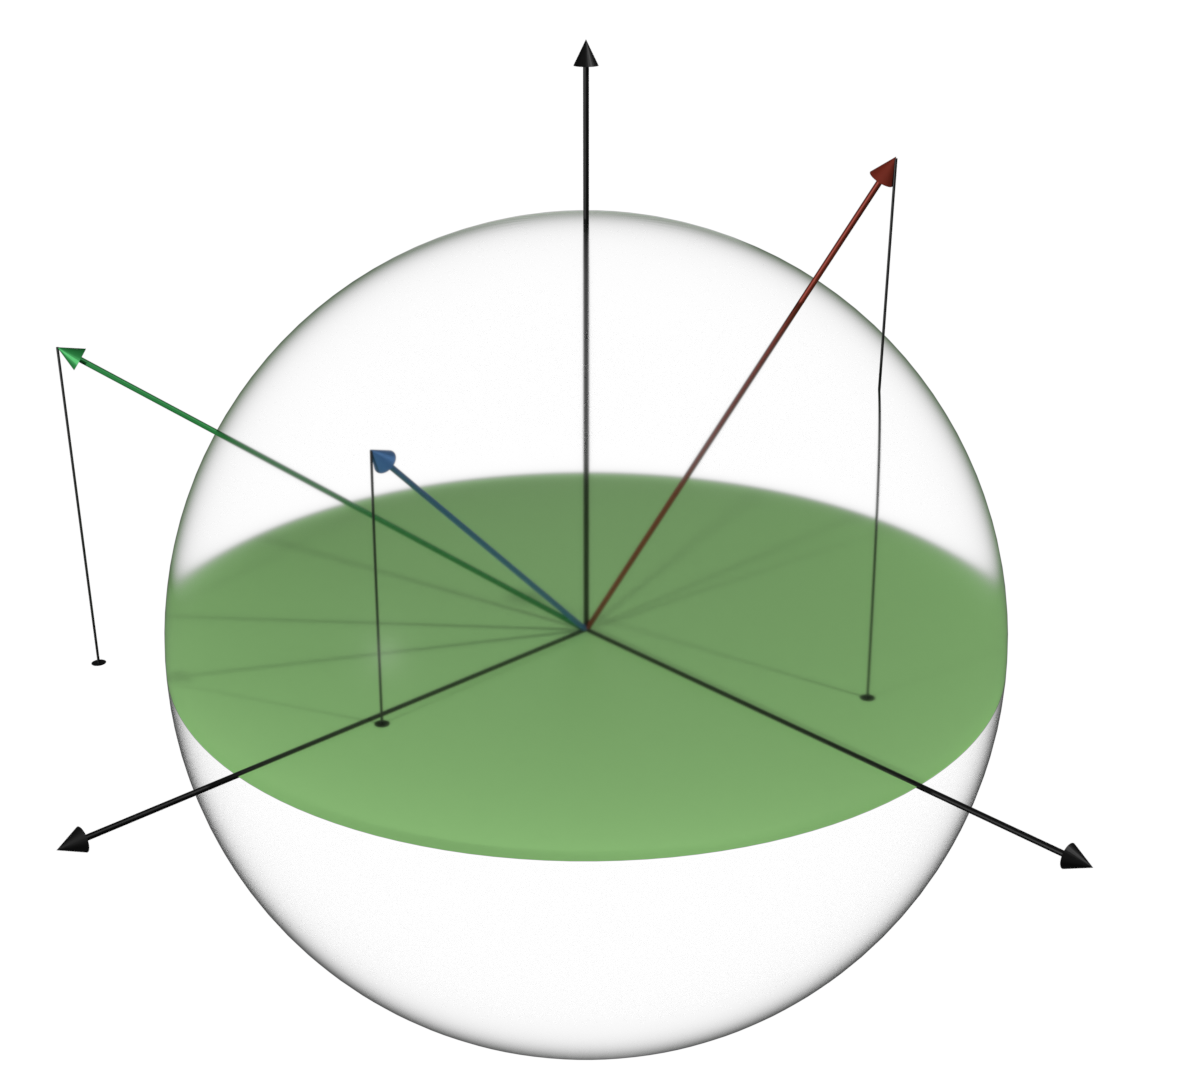
\includegraphics[width=0.75\textwidth]{figures/tiltSpherewactualWhiteBackground.png}
  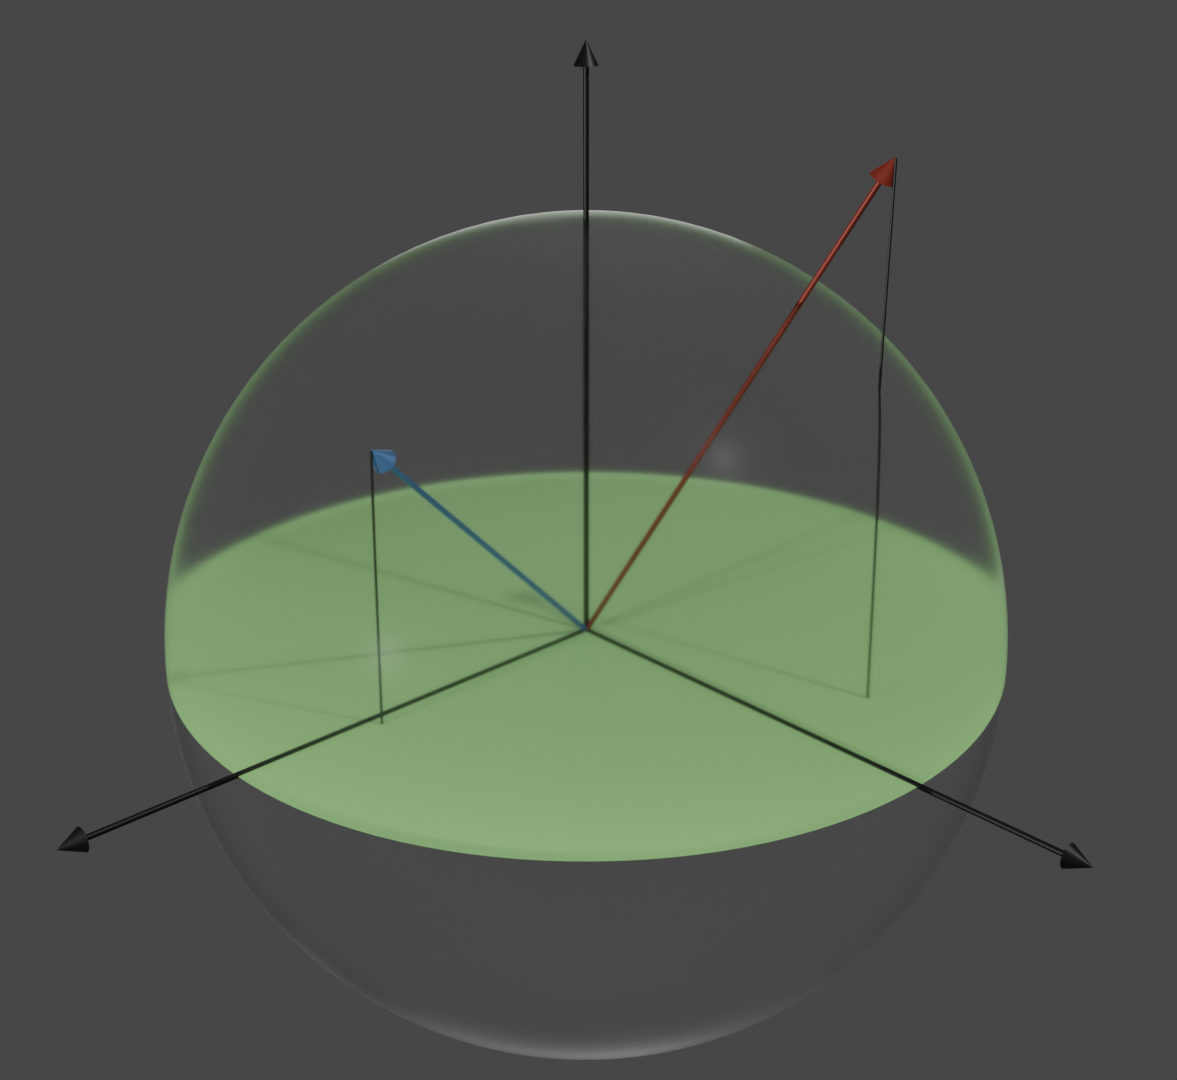
\includegraphics[width=0.75\textwidth]{figures/tiltSpherewBackground.png}
  \caption{Geometric visualization of the \emph{tilt vector} \( \vec{t} \).
    When the vector is inside the unit sphere (\( t < 1 \)), the system is in the Type-I regime.
    When the vector is outside the unit sphere (\( t > 1 \)), the system is in the Type-II regime.
    When the projection onto the \( xy \)-plane is on the unit disc, the system is in the \emph{magnetic} regime, otherwise it is in the \emph{electric} regime.
    Shown is Type-I tilt (blue), Type-II magnetic (red), and Type-II electric (green).
    Figure inspired by \textcite{tchoumakovMagneticFieldInducedRelativisticProperties2016}.
\label{fig:tiltSphere}
  }
\end{figure}

We now return to solving Eq.~\eqref{eq:32}, using the solution angle we just found.
By insertion, and after some clean up, we get
% \emph{note to thorvald: we chose \(\theta = Log \left(+ \dots\right) \)}
% \begin{multline}
%   \label{eq:39}
%   (R H_{B} R - E R^2 ) \ket{\tilde{\psi}} = 0
%   = v_F\\
%   \times \begin{pmatrix}
%           k_z ( s + t^s_z \gamma ) - E / v_F \gamma & -s ( ik_y + k_z t_x t_z \gamma - k_x / \gamma - E /v_{F} \gamma t^s_x)\\
%           s ( i k_y - k_z t_x t_z \gamma + k_x / \gamma + E /v_F \gamma t^s_x) & - k_z (s - t^s_z \gamma) - E /v_F \gamma
%         \end{pmatrix}
%     \ket{\tilde{\psi}}.
% \end{multline}
\begin{equation}
  \label{eq:39}
  (R H_{B} R - E R^2 ) \ket{\tilde{\psi}}
  = v_F  A \ket{\tilde{\psi}} = 0,
\end{equation}
with
\begin{align*}
  A_{11} &=   k_z ( s + t_{\parallel}^s \gamma ) - E / v_F \gamma,\\
  A_{12} &=  -s ( ik_y + k_z t_\perp t_\parallel \gamma - k_x / \gamma - E /v_{F} \gamma t_{\perp}^s),\\
  A_{21} &= s ( i k_y - k_z t_\perp t_\parallel \gamma + k_x / \gamma + E /v_F \gamma t_{\perp}^s),\\
  A_{22} &= - k_z (s - t_{\parallel}^s \gamma) - E /v_F \gamma.
\end{align*}
In order to simplify this further, absorb \(\gamma t_{\perp}^s (k_{z} t_{\parallel}^s - E /v_{F}) \) into \(k_{x}\).
Thus, let
\begin{equation}
  \label{eq:40}
  \begin{split}
    \tilde{k}_{x} &= k_{x} / \gamma + \gamma t_{\perp}^s ( E /v_F - k_{z} t_{\parallel}^s),\\
    \tilde{k}_{y} &=  k_{y},\\
    \tilde{k}_{z} &=  k_{z}.\\
  \end{split}
\end{equation}

These expressions warrant some explanation, as the Lorentz boost is of course
\begin{equation}
  \label{eq:41}
  \tilde{k}_x = \gamma (k_x - t_{\perp} \frac{E}{v_{F}}),
\end{equation}
where we used the four momentum \( p^{\mu } = (\frac{E}{v_{F}}, \vec{p}) \), and the effective speed of light \( v_F \).
It can thus look like our expression in Eq. \eqref{eq:40} is wrong.
The solution to this seeming inconsitency is that the proper energy is not \( \frac{E}{v_{F}} - k_z t_{\parallel} \), but rather \( \frac{E}{v_{F}} - k_z t_{\parallel} - k_x t_{\perp}\).
\todo{Something smart here, or remove discussion}

The eigenvalue equation is simply
\begin{equation}
  \label{eq:42}
  \left[  \gamma \left( t^s_{\parallel} \tilde{k}_{z} - \frac{E}{v_{F}} \right) \mathcal{I}_{2} +
  s \tilde{k}_{i} \sigma _{i} \right] \ket{\tilde{\psi}}= 0.
\end{equation}
If we now again introduce the magnetic field using minimal coupling, \(k_{x} \to  k_{x} - ey B_{z} \), this corresponds to an effective field \(B_{z} /\gamma \) in the new quantities.
This is because \(\tilde{k}_{x} \to  \tilde{k}_{x} - e y B_{z} /\gamma \).
The Landau level equation thus reads
\begin{equation}
  \label{eq:43}
  \left[
  \sum\limits_{i} s v_{F} \left(\tilde{k}_{i} + e \tilde{A}_{i} \right) \sigma _{i}
\right  ] \ket{\tilde{\psi}} =
(E- t^s_{\parallel} v_{F} \tilde{k}_{z}) \gamma \ket{\tilde{\psi}},
\end{equation}
where \(\vec{\tilde{A}}=-B_{z}/ \gamma y \hat{x}\).
We may thus use directly the result for the untilted cone, Eq.~\eqref{eq:26}, giving
\begin{subequations}
  \label{eq:44}
  \begin{align}
    \left(E - t^s_{\parallel} v_{F} \tilde{k}_{z} \right) \gamma &= \sign (m) v_{F} \sqrt{2 |m| e \frac{B}{ \gamma }  + \tilde{k}_{z}^2}, & m \neq 0,\\
    \left(E - t^s_{\parallel} v_{F} \tilde{k}_{z} \right) \gamma &= - s   \tilde{k}_{z} v_{F}, & m=0.
  \end{align}
\end{subequations}
Cleaning up, we get
\begin{subequations}
  \label{eq:45}
  \begin{align}
    E &= t^s_{\parallel} v_F \tilde{k}_{z} + \sign(m) v_F \sqrt{2 |m| e \frac{B}{\gamma ^3}  + \tilde{k}_{z}^2 /\gamma ^2}, & m\neq 0,\\
    E &= \tilde{k}_{z} v_{F} \left( t^s_{\parallel}  - s  / \gamma  \right), & m=0.
  \end{align}
\end{subequations}

As the perpendicular tilt is increased, \(\gamma = 1 / \sqrt{1-t_{\perp} ^{2}}\) diverges to infinity.
With the trivial substitution \(\alpha = 1 /\gamma \), which goes to zero, this gets an intuitive interpretation.
As the perpendicular tilt increases, the Landau levels converge towards \(t_{\parallel} v_{F} \tilde{k}_{z}\).
In particular, the separation between Landau levels is reduced by a factor \(\alpha ^{3 /2}\).
The effect of the tilt on the Landau levels is to squeeze the Landau levels together, and we will call the \(\alpha \) the \emph{squeezing factor}.
We note that when approaching the degree of tilt where we are no longer able to find a boost which enables us to solve for the Landau levels, i.e. when \( |t_{\perp}| \to 1\), the squeezing factor goes to zero.
As the tilt exceeds this limit, the squeezing factor is imaginary.
The Landau level description is only valid for \( |t_{\perp}| < 1 \).

The energy levels of the tilted cone expressed in terms of the energy levels of the untilted cone
\[
E = t^s_{\parallel} v_F k_z + \alpha E^0_{m, \alpha B},
\]
where \( E^0_{m, \alpha B} \) is the energy in the untilted case, with magnetic field \( \alpha B \).
Tilting of the Landau levels is induced by the parallel tilt component, \( t_\parallel \).
In fact, the Landau levels cross the Fermi level at the transition from Type-I to Type-II as well.
The Landau levels are shown in Figure~\ref{fig:llevelstilt}.


\begin{figure}[p!]
  \centering
  \resizebox{\textwidth}{!}{
  \newcommand{\LLplot}[2]{
  %% #1 is alpha, #2 is tz
  \addplot[forget plot]{(#2-#1) * x};  % Zeroth level
  \addplot[forget plot, black!60, dash pattern={on 3pt off 2pt on 1pt off 2pt on 1pt off 2pt on 1pt off 2pt}]{(-#2+#1) * x};  % Zeroth level, s=-1
  \addplot[forget plot, dashed]{(#2+#1) * x};  % Zeroth level, s=-1, P broken
  \addplot[forget plot, dotted]{(-#2-#1) * x};  % Zeroth level, s=1, tz<1
  \addplot[dashed, forget plot, gray] {0};
  \pgfplotsforeachungrouped \n in {1,...,5} {
    \addplot+[red, forget plot, solid] {#2 * x + #1 * sqrt(\n * #1 + x^2)};  % Positive E
    \addplot+[blue, solid] {#2 * x - #1 * sqrt(\n * #1 + x^2)};  % Negative E
  }
  \pgfplotsforeachungrouped \n in {1,...,5} {
    \addplot+[red, forget plot, dotted] {-#2 * x + #1 * sqrt(\n * #1 + x^2)};  % Positive E
    \addplot+[blue, dotted] {-#2 * x - #1 * sqrt(\n * #1 + x^2)};  % Negative E
  }
}

\tikzsetnextfilename{lllevels}
%% \hspace{-1.6cm}
\begin{tikzpicture}
  \begin{groupplot} [%
    % width=0.64\textwidth, %% Width of each window... Can be set more elegantly, but here just trial and error
    cycle list name=linestyles,
    samples=100,
    ymin=-2.5,ymax=2.5,
    xmin=-3.9, xmax=3.9,
    xlabel=\( \kappa_z \),
    ylabel=\( \epsilon_{\kappa_z m s} \),
    group style={
      x descriptions at=edge bottom,
      y descriptions at=edge left,
      horizontal sep=4pt, vertical sep=4pt,
      group size=2 by 3,
    },
    ]
    \newcommand\varalpha{1}
    \newcommand\vartz{0}
    %%
    \nextgroupplot
    \LLplot{\varalpha}{\vartz}
    \pgfmathsetmacro\hfirst{\vartz-\varalpha}
    \pgfmathsetmacro\hsecond{\vartz * 1 + \varalpha * sqrt(\varalpha + 1)}
    \draw[->] (axis cs:1,\hfirst)--(axis cs:1, \hsecond);
    %%
    \nextgroupplot
    \renewcommand\varalpha{0.6}
    \renewcommand\vartz{0}
    \LLplot{\varalpha}{\vartz}
    \pgfmathsetmacro\hfirst{\vartz-\varalpha}
    \pgfmathsetmacro\hsecond{\vartz * 1 + \varalpha * sqrt(\varalpha + 1)}
    \draw[->] (axis cs:1,\hfirst)--(axis cs:1, \hsecond);
    %%

    \nextgroupplot
    \renewcommand\varalpha{1}
    \renewcommand\vartz{0.5}
    \LLplot{\varalpha}{\vartz}
    \pgfmathsetmacro\hfirst{\vartz-\varalpha}
    \pgfmathsetmacro\hsecond{\vartz * 1 + \varalpha * sqrt(\varalpha + 1)}
    \draw[->] (axis cs:1,\hfirst)--(axis cs:1, \hsecond);
    %%
    \nextgroupplot
    \renewcommand\varalpha{0.6}
    \renewcommand\vartz{0.5}
    \LLplot{\varalpha}{\vartz}
    \pgfmathsetmacro\hfirst{\vartz-\varalpha}
    \pgfmathsetmacro\hsecond{\vartz * 1 + \varalpha * sqrt(\varalpha + 1)}
    \draw[->] (axis cs:1,\hfirst)--(axis cs:1, \hsecond);

    \pgfmathsetmacro\x{-0.8}
    \pgfmathsetmacro\gfirst{\vartz * \x - \varalpha * sqrt(1 * \varalpha + (\x)^2)}
    \pgfmathsetmacro\gsecond{\vartz * \x + \varalpha * sqrt(4 * \varalpha + (\x)^2)}
    \draw[brown, ->] (axis cs:\x,\gfirst)--(axis cs:\x, \gsecond);  %% Higher order transition
    %%
    \nextgroupplot
    \renewcommand\varalpha{1}
    \renewcommand\vartz{1.2}
    \pgfmathsetmacro\x{-sqrt(\varalpha^2/(\vartz^2-\varalpha^2))-0.3}
    \LLplot{\varalpha}{\vartz}
    \pgfmathsetmacro\hfirst{\vartz * \x + \varalpha * sqrt(\varalpha + (\x)^2)}
    \pgfmathsetmacro\hsecond{\vartz * \x + \varalpha * sqrt(2 * \varalpha + (\x)^2)}
    \draw[teal!80!black, ->, thick] (axis cs:\x,\hfirst)--(axis cs:\x, \hsecond);  %% Intraband
    %%
    \nextgroupplot
    \renewcommand\varalpha{0.6}
    \renewcommand\vartz{1.2}
    \pgfmathsetmacro\x{-sqrt(\varalpha^2/(\vartz^2-\varalpha^2))/2}
    \LLplot{\varalpha}{\vartz}
    \pgfmathsetmacro\hfirst{(\vartz - \varalpha) * \x}
    \pgfmathsetmacro\hsecond{\vartz * \x + \varalpha * sqrt(1 * \varalpha + (\x)^2)}
    \draw[->] (axis cs:\x,\hfirst)--(axis cs:\x,\hsecond);
  \end{groupplot}
\end{tikzpicture}

  }
  % \includegraphics[width=0.8\textwidth]{example-image-10x16}
  \caption{\label{fig:llevelstilt}Landau levels for different values of \( t_x, t_z \).
    The top two rows show Type-I, while the lowest row shows Type-II.
    Left column shows \( t_x = 0 \), right column \( t_x = 0.64 \) (\( \alpha = 0.6 \)).
    The rows shows \( t_z = 0, 0.5, 1.2 \), from top to bottom.
    The dotted lines show the Landau levels with opposite sign of \( t_z \), the dashed show the opposite chirality.
    The arrows indicate valid ``transitions'', namely the \( 0\to 1 \) interband in black, \( -1 \to 4 \) interband in \textcolor{brown!70!black}{brown}, and \( 1\to 2 \) intraband in \textcolor{teal!70!black}{teal}.
  }
\end{figure}

The eigenstate of
\[
H = v_{F} \sigma ^{i} ( p_{i} + e A_{i} ),
\]
with \(A_{i} = - B_{z} y \delta _{i x}\), given in the position basis, is
\begin{equation}
  \phi _{\vec{k} m s}(\vec{r}) = \frac{1}{\sqrt{L_xL_z}}
  \frac{e^{ik_x x}e^{ik_z z}}{\sqrt{\alpha_{k_z m s}^2 + 1}}
  e^{-\frac{y-k_x l^2}{2 l_B^2}}
  \begin{pmatrix}
    \frac{\alpha_{k_z m s}}{\sqrt{2^{M-1} (M-1)! \sqrt{\pi } l_B}} H_{M-1}\left( \frac{y-k_x l_B^2}{l_B} \right)\\
    \frac{1}{\sqrt{2^M M! \sqrt{\pi } l_B}} H_M \left( \frac{y-k_x l_B^2}{l_B} \right)
  \end{pmatrix},
\end{equation}
where capital letters indicate absolute value of corresponding quantity, $M=|m|, \vec{k} = (k_x, k_z)$, and with the normalization factor
\begin{equation}
  \alpha_{k_z m s} = \frac{-\sqrt{2eB M}}{\frac{E_{k_z m s}}{s v_{F}} -   k_z}.
\end{equation}
Taking care to keep track of boosted and rescaled quantites, the eigenstate in the boosted frame is
\begin{equation}
  \label{eq:47}
  \tilde{\psi}(\tilde{\vec{r}}) =
  \frac{1}{\sqrt{L_xL_z}}
  \frac{e^{i \tilde{k}_x \tilde{x}}e^{i k_z z}}{\sqrt{\alpha_{\tilde{k}_z m s}^2 + 1}}
  e^{-\frac{\left(\tilde{y} - \tilde{k}_x l_{B'}^2\right)^2}{2 l_{B'}^2}}
  \begin{pmatrix}
    \frac{\alpha_{\tilde{k}_z m s}}{\sqrt{2^{M-1} (M-1)! \sqrt{\pi } l_{B'}}} H_{M-1}\left( \frac{\tilde{y} - \tilde{k}_x l_{B'}^2}{l_{B'}} \right)\\
    \frac{1}{\sqrt{2^M M! \sqrt{\pi } l_{B'}}} H_M \left( \frac{\tilde{y} - \tilde{k}_x l_{B'}^2}{l_{B'}} \right)
  \end{pmatrix},
\end{equation}
with
\begin{equation}
  \alpha_{\tilde{k}_z m s} = \frac{-\sqrt{2e B'  M}}{ \gamma \frac{E_{\tilde{k}_z m s} - t^s_{\parallel} v_{F} \tilde{k}_{z}}{s v_{F}} -   \tilde{k}_z},
\end{equation}
where
\[
B' = B \alpha.
\]
We note that \( \alpha_{k_z 0 s} = 0 \), so using the explicit form of the energy we may simplify the expression some.
For \( m\neq 0 \)
\[
  \frac{
    E_{k_z m s} - t^s_{\parallel} v_F k_z
  }{s v_{F}} = \sign(m) s \alpha \sqrt{2 M e B \alpha + k_{z}^2}
\]
and thus
\begin{equation}
  \label{eq:48}
  \alpha_{k_z m s} =
  \frac{-\sqrt{ \alpha M }}{\sign(m) s \sqrt{\alpha M + \kappa^2} - \kappa}
\end{equation}
where we defined the dimensionless \( \kappa_z = \sqrt{2 e B} k_z  \).

The original eigenstate \(\ket{\psi } = 1 /\mathcal{N} e^{\theta /2 \sigma _{x}} \ket{\tilde{\psi} }\) of the tilted system is easily found.
Reinserting explicitly, in the boosted frame, that
\[
  \tilde{k}_{x} = \alpha k_{x} + \frac{t_{\perp}^s}{\alpha} (E_{k_z m s} /v_F- k_{z} t_{\parallel}^s)
  = \alpha k_x + t_{\perp}^s \frac{E^0_{m, \alpha B} }{v_{F}}
\]
and \(l_{B'}=\frac{l_{B}}{\sqrt{\alpha} }\)
we define
\begin{equation}
  \label{eq:49}
  \chi =
  \frac{y-\tilde{k}_{x} l_{B'}^2}{l_{B'}}
  =
  \sqrt{\alpha } (y-k_{x} l_{B}^2) /l_{B}
  + \frac{ t_{\perp}^s l_B }{ \sqrt{\alpha} v_F} E^{0}_{m, \alpha B},
\end{equation}
which is the argument of the Hermite polynomials.
For later convenience, let us explicitly define
\begin{equation}
  \label{eq:50}
  \tilde{\phi} _{\vec{k} m s} (\vec{\tilde{r}}) =
  \frac{e^{i \tilde{k}_{x} \tilde{x} + i k_{z} z}}{\sqrt{L_{x} L_{z}} }
  \underbrace{
  \frac{
    e^{-\frac{1}{2} \chi ^2}
    \sqrt[4]{\alpha }
  }
  {\sqrt{\alpha^2_{\tilde{k}_{z} m s} + 1} }
  \begin{pmatrix}
    \frac{\alpha_{\tilde{k}_z m s}}{\sqrt{2^{M-1} (M-1)! \sqrt{\pi } l_{B}}} H_{M-1}\left( \chi  \right)\\
    \frac{1}{\sqrt{2^M M! \sqrt{\pi } l_{B}}} H_M \left( \chi \right)
  \end{pmatrix}}_{\tilde{\phi}_{\vec{k} m s} (y)},
\end{equation}
and thus
\begin{equation}
  \label{eq:51}
  \tilde{\phi}_{\vec{k} m s} (y) =
  e^{-\frac{1}{2} \chi ^2}
  \begin{pmatrix}
    a_{\vec{k} m s} H_{M-1} (\chi)\\
    b_{\vec{k} m s} H_{M} (\chi)
  \end{pmatrix},
\end{equation}
with
\begin{align}
 \label{eq:52}
  a_{\vec{k} m s} &=
                    \frac{
                    \alpha_{\tilde{k}_z m s} \sqrt[4]{\alpha }
                    }{
                    \sqrt{\alpha^2 _{\tilde{k}_z m s} + 1}
                    \sqrt{2^{M-1} (M-1)! \sqrt{\pi} l_B}
                    },\\
  \label{eq:53}
  b_{\vec{k} m s} &=
                    \frac{
                     \sqrt[4]{\alpha }
                    }{
                    \sqrt{\alpha^2 _{\tilde{k}_z m s} + 1}
                    \sqrt{2^{M} M! \sqrt{\pi} l_B}
                    }.
\end{align}

We proceed now to find the normalization factor \( \mathcal{N} \), as it will become necessary in later steps.
Recall that
\[
  \ket{\psi} = \frac{1}{\mathcal{N}} e^{\theta /2 \sigma _x} \ket{\tilde{\psi}},
\]
and
\[
e^{\theta \sigma _x} =
\frac{1}{\alpha }
\begin{pmatrix}
  1 & -s t_{\perp}^s\\
  -s t_{\perp}^s & 1
\end{pmatrix}.
\]
The upper and lower part of the spinor are orthogonal, thus we have
\begin{equation}
  \label{eq:54}
  \braket{\psi  | \psi } = \frac{1}{\mathcal{N}^{*} \mathcal{N}} \frac{1}{\alpha } \braket{\tilde{\psi}  | \tilde{\psi} } = 1 \implies \mathcal{N}^{*}\mathcal{N} = \frac{1}{\alpha }.
\end{equation}
We choose \( \mathcal{N} = \alpha^{-\frac{1}{2}} \).

\begin{summary}\label{summary:llevels}
The tilted Hamiltonian
  \[
    H = v_F \vec{t}^s \vec{p} + s v_F \vec{p} \vec{\sigma}
  \]
  in a magnetic field \( \vec{B} \) has the Landau levels
  \[
    E =
    \begin{cases}
      t^s_{\parallel} v_F k_z + \sign(m) v_F \alpha \sqrt{2 e B \alpha M + k_{z} ^2} & m \neq 0,\\
      t^s_{\parallel} v_F k_z - s \alpha v_F k_z & m = 0,
    \end{cases}
  \]
  with the the \emph{squeezing factor} \( \alpha = \sqrt{1 - t_{\perp} ^2}  \).
  The associated eigenstates in the position basis are
  \[
    \psi(\vec{r}) = \sqrt{\alpha} e^{\theta /2 \sigma_x}
    \frac{
      e^{ik_{x} x + ik_{z} z}
    }{
      \sqrt{L_{x}  L_z}
    } \tilde{\psi}(y),
    \]
    where
    \[
      \tilde{\psi} (y) = e^{-\frac{1}{2} \chi^2}
      \begin{pmatrix}
        a_{k_z m s} H_{M - 1} (\chi) \\
        b_{k_z m s} H_M (\chi)
      \end{pmatrix},
    \]
    where we have defined \( \chi = \sqrt{\alpha} \frac{ y - k_x l_B^2 }{l_{B}} + \frac{t_{\perp}^s l_B}{\sqrt{\alpha} v_{F}} E^0_{m, \alpha B} \) and \( a_{k_z m s}, b_{k_z m s} \) are given in Eqs.~(\ref{eq:52}, \ref{eq:53}).
\end{summary}

\section{Analytical expression for the response function}
We will here find analytical expressions for the current operator $J^i(\omega, \vec{q})$ and energy-momentum tensor $T^{j 0}(\omega, \vec{q})$, needed to calculate the correlation function.
The fields are given, in the position basis, by
\begin{align}
  \psi &= \sum\limits_{\vec{k}n}^{}\braket{\vec{r} | \vec{k} n s} a_{\vec{k}ns}(t) = \sum\limits_{\vec{k}n}^{} \phi_{\vec{k} n s} (\vec{r}) a_{\vec{k}n s}(t),\\
  \psi^{\dagger} &= \sum\limits_{\vec{k}n}^{}
                   \braket{\vec{k} ns | \vec{r} }
                   a^{\dagger}_{\vec{k}ns}(t)
                   =\sum\limits_{\vec{k}n}^{} \phi^{*}_{\vec{k} n s} (\vec{r}) a^{\dagger}_{\vec{k}n s}(t).
\end{align}
\todo{Is the asterisk supposed to be dagger? \( \phi^{*} \to \phi^{\dagger} \) as it must be transpose??}
Here $a_{\lambda }^{\dagger} (t) = \exp(iE_{\lambda } t / ) a_{\lambda }^{\dagger}$ and $a_{\lambda }^{\dagger}, a_{\lambda }$ are the creation and annihilation operators of the state with quantum numbers $\lambda $.
\subsection{Expressions for the operators}
\subsubsection{The current operator}
The current operator $\hat{\vec{J}} = e \hat{\vec{v}}$, where $\hat{\vec{v}}$ is the velocity operator.
Using the relation of Heisenberg operators $\dot{A} = -i [A, H] $~\cite{sakuraiModernQuantumMechanics2017}, for the operator $A$ and Hamiltonian $H$, and with the minimal coupling \( \vec{p}^B = \vec{p} + e \vec{A} \),
\begin{align}
  \vec{v} = \dot{\vec{r}} &= -i \left[ \vec{r}, H \right]\\
  &= -i v_F (s \sigma^i + (t^s)^i) \left[\vec{r}, p^B_i\right]\\
  &= v_F (s \vec{\sigma} + \vec{t}^s),
\end{align}
where we used the canonical commutation relation \( [r_i, p_j] = i \delta_{ij} \) and the commutation between the position operator and magnetic potential \( \vec{A} \).
We thus get
\begin{equation}
  J^x = \psi ^{\dagger} \hat{J}^x \psi = sv_F e \sum\limits_{\vec{k}m, \vec{l}n}^{}
  \phi _{\vec{k}ms}^{*}(\vec{r}) \left(\sigma^x + s t^s_x\right) \phi _{\vec{l}ns}(\vec{r})
  a_{\vec{k}ms}^{\dagger}(t)
  a_{\vec{l}ns}(t).
\end{equation}

\subsubsection{The energy-momentum tensor}
The \emph{canonical} energy-momentum tensor is generally defined by
\begin{equation}
  \label{eq:55}
  T^{\mu \nu} =  \frac{\delta \mathcal{L}}{\delta(\partial_{\mu} \phi_{i})} \partial_{\nu} \phi_i - \eta^{\mu \nu} \mathcal{L},
\end{equation}
where the index \( i \) runs over the types of fields.
This definition is correct for commuting fields, however, for non-commuting fields like ours, this formula is slightly wrong.
This is often overlooked in many textbooks and papers, so we will here elucidate the issue to some degree.
While a proper derivation requires the use of Grassman variables and defining left and right derivation, which we will not do here, some simple considerations help in understanding the issue.
In the standard textbook derivation of the canonical energy-momentum tensor, one expands the total derivative of the Lagrangian \( \mathcal{L}(\psi_i, \partial \psi_i)\) in terms of the fields,
\begin{equation}
  \label{eq:56}
  \frac{\mathrm{d} \mathcal{L}(\psi_{i}, \partial \psi_i)}{\mathrm{d} x_{\nu }} \equiv \mathrm{d}^{\nu } \mathcal{L}
  = \frac{\partial \mathcal{L}}{\partial (\partial_{\mu } \phi_i)} \frac{\partial(\partial _{\mu } \psi_i)}{\partial x_{\nu }}
  + \frac{\partial \mathcal{L}}{\partial \psi _{i}} \frac{\partial \psi_i}{\partial x_{\nu }}.
\end{equation}
This expansion, however, ignores the non-commutative nature of the fields.
For concreteness, consider \( \psi _i = \bar{\psi} \).
Heuristically, the correct expression would be obtained by reordering the factors in the two terms.
By naively employing \cref{eq:55}, the resulting canonical energy-momentum tensor of the Dirac theory would be
\begin{equation}
  T^{\mu \nu} = \frac{\delta \mathcal{L}}{\delta (\partial_{\mu} \bar{\psi})} \partial^{\nu} \bar{\psi}  + \frac{\delta \mathcal{L}}{\delta (\partial_{\mu} \psi)} \partial^{\nu} \psi - \eta^{\mu \nu} \mathcal{L},
\end{equation}
while the correct form is~\cite[Eq.~3-153]{itzyksonQuantumFieldTheory1980}
\begin{equation}
  \label{eq:57}
  T^{\mu \nu} = \partial^{\nu} \bar{\psi} \frac{\delta \mathcal{L}}{\delta (\partial_{\mu} \bar{\psi})} + \frac{\delta \mathcal{L}}{\delta (\partial_{\mu} \psi)} \partial^{\nu} \psi - \eta^{\mu \nu} \mathcal{L}.
\end{equation}

The untilted Weyl Hamiltonian
\begin{equation}
  H_s = s \sigma^i p_i,
\end{equation}
where natural units (\( c = v_F = 1 \)) are used, to have the expressions explicitly match those of \gls{qft} literature;
the associated Lagrange density~\cite{kachelriessQuantumFieldsHubble2018}
\begin{equation}
  \mathcal{L}_s = i \phi^{\dagger} \sigma_s^{\mu} \partial_{\mu} \phi,
\end{equation}
with \( \sigma_s^{\mu} = (I_2, s \vec{\sigma}) \), i.e. \( \sigma_{s=1}^{\mu} = \sigma^{\mu}, \sigma_{s=-1}^{\mu} = \bar{\sigma}^{\mu} \) known from the Dirac solutions.
This is seen directly from the Dirac Lagrangian \( i \bar{\psi} \slashed{\partial} \psi \) by taking \( \psi = (\phi_L, \phi_R)^T \) and setting, for example, \( \phi_R = 0 \).
Symmetrize in daggered and undaggered fields
\footnote{The Lagrangian itself is nonphysical, and we may transform it in any way that leaves the action \( \int \mathcal{L} \) invariant.}
\begin{equation}
  \mathcal{L}_s = \frac{i}{2} (\phi^{\dagger} \sigma_s^{\mu} \partial_{\mu} \phi - \partial_{\mu} \phi^{\dagger} \sigma_s^{\mu} \phi),
\end{equation}
which will prove more convenient to work with.
From the definition of the canonical energy-momentum tensor for Dirac fields \cref{eq:57}, one gets
\begin{equation}
  T^{\mu \nu} =
  \frac{i}{2} (
  \phi^{\dagger} \sigma_s^{\mu} \partial_{\nu} \phi
  - \partial_{\nu} \phi^{\dagger} \sigma_s^{\mu} \phi
  - \eta^{\mu \nu} \mathcal{L}
  ).
\end{equation}
Consider now the tilted Weyl Hamiltonian
\begin{equation}
  H_s = s \sigma^ik_i + (t^s)^i p_i.
\end{equation}
Exactly analogous to the treatment of~\textcite{vanderwurffMagnetovorticalThermoelectricTransport2019} for the full \( 4 \times 4 \) tilted Dirac Lagrangian, absorb the tilt term into the Pauli matrices, giving the Lagrangian density
\begin{equation}
  \mathcal{L}_s = i \phi^{\dagger} \tilde{\sigma}_s^{\mu} \partial_{\mu} \phi,
\end{equation}
where \( \tilde{\sigma}_s^{\mu} = \sigma_s^{\mu} + (t^s)^{\mu}, \; (t^s)^{\mu} = (0, \vec{t^s}) \).
The corresponding energy-momentum tensor, after again symmetrizing in the fields,
\begin{equation}
  \label{eq:T-canon-tilt}
  T^{\mu\nu} =
  \frac{i}{2} (
  \phi^{\dagger} \tilde{\sigma}_s ^{\mu} \partial_{\nu} \phi
  - \partial_{\nu} \phi^{\dagger} \tilde{\sigma}_s ^{\mu} \phi
  - \eta^{\mu \nu} \mathcal{L}
  ).
\end{equation}
Reintroducing the explicit effective speed of light \( v_F \) and recalling \( \partial_0 = \partial_t / v_F \) this gives
% \begin{comment}
% The untilted Weyl Hamiltonian
% \[
% H_s = s \sigma^i k_i
% \]
% may of course be considered a Weyl decomposition of a full massless Dirac equation.

% \todo{Why do we have to consider 4x4? Is the definitions not also valid for 2x2?}
% \todo{Regarding the non-symmetry of the stress tensor, see keichelriess eq 5.16 with discussion}

% The untilted Weyl Hamiltonian
% \[
% H_s = s \sigma^i k_i
% \]
% can be considered the Hamiltonian of one part of a Weyl decomposition of a Dirac system.
% The Weyl field has the Lagrangian density~\cite{kachelriessQuantumFieldsHubble2018}
% \begin{equation}
%   \label{eq:58}
%   \mathcal{L} = i \phi^{\dagger} \sigma^{\mu} \partial_{\mu} \phi,
% \end{equation}
% which may be seen directly from the Dirac Lagrangian \( i \bar{\psi} \slashed{\partial } \psi  \) by taking \( \psi = (\phi_L, \phi_R)^T \) and set, for example, \( \phi _R = 0 \).
% Symmetrizing in daggered and undaggered fields
% \footnote{The Lagrangian itself is unphysical, and we may transform it in any way that leaves the action \( \int \mathcal{L} \) invariant.}
% \todo{Alternatively argue by directly showning that this does not affect the action by doing an integration by parts}
% \[
%   \mathcal{L} = \frac{i}{2} \left(\phi^{\dagger} \sigma^{\mu} \partial_{\mu} \phi - \partial_{\mu} \phi^{\dagger} \sigma^{\mu} \phi \right),
% \]
% which will prove to be more convenient to work with.
% Adapting the definition \cref{eq:57} the energy-momentum tensor for the untilted Dirac cone is thus
% \begin{equation}
%   \label{eq:59}
%   T^{\mu \nu} =
%   \frac{i}{2} (
%   \phi^{\dagger} \sigma^{\mu} \partial_{\nu} \phi
%   - \sigma^{\mu} \phi \partial_{\nu} \phi^{\dagger}
%   - \eta^{\mu \nu} \mathcal{L}
%   ).
% \end{equation}

% Moving now to the tilted case, the 4x4 Lagrangian becomes~\cite{vanderwurffMagnetovorticalThermoelectricTransport2019}
% \todo{check sign compared to action in stoof}
% \begin{equation}
%   \label{eq:60}
%   \mathcal{L}_{\text{tilt}} = i \bar{\psi} \Gamma ^{\mu }\partial_{\mu } \psi ,
% \end{equation}
% where we have introduced modified gamma matrices
% \begin{equation}
%   \label{eq:61}
%   \Gamma ^{\mu } =
%   \begin{cases}
%     \gamma ^{\mu } + t^{\mu} \gamma ^0& \text{ inversion symmetry broken},\\
%     \gamma^{\mu} + t^{\mu} \gamma^0 \gamma^5 & \text{ inversion symmetric},
%   \end{cases}
% \end{equation}
% with \( t^{\mu } = (0, \vec{t}) \).
% Decomposing to \( 2\times 2 \), this yields
% \begin{equation}
%   \label{eq:62}
%   T^{\mu \nu} =
%   \frac{i}{2} (
%   \phi^{\dagger} \tilde{\sigma} ^{\mu} \partial_{\nu} \phi
%   - \tilde{\sigma} ^{\mu} \phi \partial_{\nu} \phi^{\dagger}
%   - \eta^{\mu \nu} \mathcal{L}
%   ),
% \end{equation}
% where we defined the modified Pauli matrices
% \begin{equation}
%   \label{eq:63}
%   \tilde{\sigma}^{\mu} =
%   \begin{cases}
%     \sigma^{\mu} + t^{\mu} & \text{ inversion symmetry broken},\\
%     \sigma^{\mu} + s t^{\mu} & \text{ inversion symmetric}.
%   \end{cases}
% \end{equation}
% \end{comment}
% \begin{equation}
%   \begin{split}
%     T^{y_0}(t, \vec{r}) &=
%     \sum\limits_{\vec{k} m, \vec{l} n}^{}
%     \frac{1}{2}
%     \bigg\{
%     \phi ^{*}_{\vec{k} m s}(\vec{r}) (s \sigma^y + (t^s)^y) \phi _{\vec{l} n s }(\vec{r})\\
%     & \times \left[
%       a^{\dagger}_{\vec{k} m s}(t) i \partial_t  a_{\vec{l} n s}(t)
%       -
%       i \left(\partial_t a^{\dagger}_{\vec{k} ms }(t) \right) a_{\vec{l} n s}(t)
%     \right]\\
%       &+ \phi ^{*}_{\vec{k} m s}(\vec{r}) (s \sigma^y + (t^s)^y) 2\mu \phi _{\vec{l} n s}(\vec{r}) a^{\dagger}_{\vec{k} m s}(t) a_{\vec{l} n s}(t)
%     \bigg\}.
%   \end{split}
% \end{equation}
\begin{multline}
    T^{y_0}(t, \vec{r}) =
    \frac{1}{2}
    \sum\limits_{\vec{k} m, \vec{l} n}^{}
    \phi ^{*}_{\vec{k} m s}(\vec{r}) (s \sigma^y + (t^s)^y) \phi _{\vec{l} n s }(\vec{r})\\
    \times \left[
      a^{\dagger}_{\vec{k} m s}(t) i \partial_t  a_{\vec{l} n s}(t)
      -
      i \left(\partial_t a^{\dagger}_{\vec{k} ms }(t) \right) a_{\vec{l} n s}(t)
      -  2\mu  a^{\dagger}_{\vec{k} m s}(t) a_{\vec{l} n s}(t)
        \right].
\end{multline}
Here, also a non-zero potential $\mu $ is included by hand%
\footnote{This is of course in no way a rigorous treatment of the chemical potential. Heuristically, one may argue that as the \( T^{y0} \) component is to be regarded as the energy flux, the contribution from chemical potential should be the chemical potential multiplied by the particle velocity operator. },%
\todo{The footnote makes the definition sound much like heat current (see Mahan eq. 3.484)}
equal to what was done in~\textcite{arjonaFingerprintsConformalAnomaly2019}.
% Our final result will be given at zero potential, however, it is included in the calculations as it is later interesting to consider small deviations from zero chemical potential.
Our final result will be given at zero potential, however, it is included in the calculations as it for future work is interesting to consider small deviations from zero chemical potential.
Recalling the time dependence of $a(t), a^{\dagger}(t)$ we have that
\[
  i \partial_t a_{\lambda }(t) = E_{\lambda }a_{\lambda },
  \quad
  i \partial_t a^{\dagger}_{\lambda }(t) = -E_{\lambda }a^{\dagger}_{\lambda },
\]
which further simplifies the expression.

\begin{summary}
  The current- and energy-momentum tensor operator are
  \begin{align}
    J^x &= sv_F e \sum\limits_{\vec{k}m, \vec{l}n}^{}
          \phi _{\vec{k}ms}^{*}(\vec{r}) \left(\sigma^x + s t^s_x\right) \phi _{\vec{l}ns}(\vec{r})
          a_{\vec{k}ms}^{\dagger}(t)
          a_{\vec{l}ns}(t),\\
    T^{y_0}(t, \vec{r}) &=
                          \frac{1}{2}
                          \sum\limits_{\vec{k} m, \vec{l} n}^{}
                          \phi ^{*}_{\vec{k} m s}(\vec{r}) (s \sigma^y + (t^s)^y) \phi _{\vec{l} n s }(\vec{r})\\
\nonumber        &\times \left[
                   E_{k_z m s} + E_{l_z n s} - 2\mu \right]
                   a^{\dagger}_{\vec{k} m s}(t)  a_{\vec{l} n s}(t).
  \end{align}
\end{summary}

\begin{comment}
  The energy-momentum tensor of the massles \gls{qed}
  \begin{equation}
    \label{eq:64}
    \mathcal{L} = -\frac{1}{4} F^{\mu \nu }F_{\mu \nu } + \overline{\psi} i \slashed{D} \psi
  \end{equation}
  is given by~\cite{chernodubGenerationNernstCurrent2018}
  \begin{equation}
    T^{\mu \nu } = -F^{\mu \nu } F_{\mu \nu } + \frac{1}{4} \eta ^{\mu \nu } F_{\alpha \beta } F^{\alpha \beta } + \frac{i}{2} \overline{\psi}
    \left( \gamma ^{\mu } D^{\nu } + \gamma ^{\nu } D^{\mu } \right) \psi
    - \eta ^{\mu \nu } \overline{\psi} i \slashed{D} \psi .
  \end{equation}
  Specializing to the Weyl Hamiltonian we may drop the terms originating with the $F$ field self energy, and also we will consider only one Weyl spinor part of the Dirac four spinor.
  Thus, the energy-momentum tensor is given by
  \begin{equation}
    T^{\mu \nu } = \frac{i}{2} \psi ^{\dagger} \left( \sigma ^{\mu } D^{\nu } + \sigma ^{\nu } D^{\mu } \right) \psi  - \eta ^{\mu \nu } \psi ^{\dagger} i \sigma ^{\mu } D_{\mu } \psi ,
    \label{eq:65}
  \end{equation}
  where $\psi $ is to be understood as the solutions found above, $D_{\mu }=\partial _{\mu }  - i e A_{\mu }$ is the covariant derivative, and $\sigma ^{\mu } = (I, \sigma ^i)$
  In our calculations we will require the $T^{y 0}$ component, which we will now find.

  By using \cref{eq:65} directly
  \begin{align}
    T^{y 0} &= \frac{i}{2} \psi ^{\dagger} \left( D^{y} + \sigma ^{y} D^{0} \right)\psi \\
           &= \frac{i}{2} \psi ^{\dagger} \left( \partial ^{y} + \sigma ^{y} \partial ^{0} \right)\psi \\
           &= \frac{i}{2} \left[
             \phi ^{*} \sigma ^y \phi  a^{\dagger} \partial ^0 a + \phi ^{*} \left( \partial ^y\phi  \right) a^{\dagger}a
             \right].
  \end{align}
  The energy-momentum tensor is obviously real, thus
  \[
    T^{y 0} = \frac{1}{2} \left( T^{y 0} + \left(  T^{y 0}\right)^{\dagger} \right),
  \]
  which after evaluation gives
  \begin{equation}
    T^{y 0} =  \frac{i}{4} \left[
      \phi ^{*} \sigma ^y \phi \left( a^{\dagger} \partial ^0 a - (\partial ^0a)^{\dagger} a \right)
      +
      \left(
        \phi ^{*} \partial ^y \phi  - \left( \partial ^y \phi  \right)^{\dagger} \phi 
      \right)
      a^{\dagger}a
    \right].
  \end{equation}
  Now, recovering our dimensionfull quantities by letting $i\partial_{\mu }  \to v_F p_{\mu }$ \todo{what happens to s?}, which we see from comparing the \gls{qed} Lagrangian in \cref{eq:64} to our system.
  The four momentum is given as usual, with $c \to v_F$, by $p_{\mu } = \left( \frac{E}{v_{F}}, -\vec{p} \right) =  (i\frac{\partial_0}{v_{F}}, -p _i)$.
  This gives the final expression 
  \begin{equation}
    T^{y 0} =  \frac{1}{4} \left[
      \phi ^{*} \sigma ^y \phi \left( a^{\dagger} i \partial ^0 a - (i \partial ^0a)^{\dagger} a \right)
      - v_{F}
      \left(
        \phi ^{*} p^y \phi  - \left( p^y \phi  \right)^{\dagger} \phi 
      \right)
      a^{\dagger}a
    \right].
  \end{equation}
\end{comment}


\subsection{Response function in momentum space}
Fourier transforming the position gives
\begin{align}
  \label{eq:66}
  J^x(t, \vec{q}) &= \sum\limits_{\vec{k}m, \vec{l}n}
                    J^x_{\vec{k}ms, \vec{l}ns}(\vec{q})
                    a^{\dagger}_{\vec{k}ms}(t)
                    a_{\vec{l} ns}(t),\\
  \label{eq:67}
  T^{y 0}(t, -\vec{q}) &= \sum\limits_{\vec{k}m, \vec{l}n}^{}
                    T^{y 0}_{\vec{k}m s, \vec{l}n s}(\vec{q})
                    a^{\dagger}_{\vec{k}m s}(t)
                    a_{\vec{l} n s}(t),
\end{align}
where the matrix elements in momentum space are given by
\begin{align}
  J^x_{\vec{k}ms, \vec{l}ns}(\vec{q}) &=  \int \mathrm{d} \vec{r} e^{-i \vec{q} \vec{r}} s v_F e \phi ^{*}_{\vec{k}ms} (\vec{r}) (\sigma^x + s t^s_x) \phi _{\vec{l}ns}(\vec{r}),\\
  %%
  \label{eq:68}
  T^{y 0}_{\vec{k}m s, \vec{l} n s}(\vec{q}) &= \frac{1}{2}
                                                \int \mathrm{d}\vec{r} e^{i\vec{q}\vec{r}}
                                              \phi ^{*}_{\vec{k}m s}(\vec{r})
                                              (s \sigma ^y + (t^s)^y)
                                                (E_{\vec{k}_z m s} + E_{\vec{l}_z n  s} - 2 \mu ) \phi _{\vec{l} n  s}(\vec{r}).
\end{align}
Note that as $T^{y 0}(t, -\vec{q})$ will be used later, we here for convenience included the sign into the definition of the matrix element  $T^{y 0}_{\vec{k}ms, \vec{l}ns}$, as is reflected in the sign of the exponent of \cref{eq:68}.

As was noted earlier, the eigenvectors are plane waves in the \( x \)- and \( z \)-directions, and the non-trivial part is the $y$-dependent $\phi (y)$.
Thus, we want to express these matrix elements in terms of $\phi (y)$.
The sum over $\vec{l}$ in \cref{eq:66} can be replaced by an integral, as it is a good quantum number.
As usual, the measure in the integration is given by the density of states in momentum space, the well-known $L_{i} /2\pi $, with $L_i$ being the length of the system in the $i$-direction.
\begin{align}
  J^x(t, \vec{q}) &= \sum\limits_{\vec{k}m, n}^{} \int \mathrm{d}l_x \mathrm{d}l_z \frac{L_xL_z}{4 \pi ^2}
                    J^x_{\vec{k}ms, \vec{l}ns} (\vec{q}) a^{\dagger}_{\vec{k} ms} (t) a_{\vec{l} ns}(t)\\
  \nonumber &= \int \mathrm{d}l_x \mathrm{d} l_{z} \int \mathrm{d} y e^{-i q_y y}
                    \delta (l_x - k_x - q_x) \delta (l_z - k_z -  q_z)\\
                    \nonumber &\pe \times sv_F e \phi ^{*}_{\vec{k} ms}(y) (\sigma^x + s t^s_x) \phi _{\vec{l}ns}(y).
\end{align}
The Dirac delta functions appeared from taking the integrals from the matrix element over $x$ and $z$, as the integrand in these variables was only plane waves.
The exact same procedure may be done for the energy-momentum tensor in \cref{eq:67}.
Eliminating $l$ by doing the integrals yields
\begin{align}
  J^x(t, \vec{q}) &= \sum\limits_{\vec{k}, mn}^{}
                    J^x_{\vec{k}ms, \vec{k}+\qvec{q} ns}(\vec{q}) a^{\dagger}_{\vec{k} ms}(t) a_{\vec{k}+\qvec{q} ns}(t),\\
  T^{y 0}(t, -\vec{q}) &= \sum\limits_{\vec{\kappa}, \mu  \nu }^{} T^{y 0}_{\vec{\kappa } \mu  s, \vec{\kappa } - \qvec{q}, \nu  s}(\vec{q}) a^{\dagger}_{\vec{\kappa } \mu   s}(t) a_{\vec{\kappa } - \qvec{q} \nu  s}(t),
\end{align}
where ${\qvec{q}} = (q_x, q_z)$.
Keeping in mind that $a_{\lambda }^{\dagger} (t) = e^{i E_{\lambda } t /  }a_{\lambda }^{\dagger}$, and that
\begin{equation}
  \Braket{\left[
a^{\dagger}_{\vec{k}ms} a_{\vec{k}+\qvec{q} ns}, a^{\dagger}_{\vec{\kappa}\mu s} a_{\vec{\kappa}-\qvec{q} \nu  s}
\right]}
=
\delta_{\vec{k}, \vec{\kappa}-\qvec{q}}
\delta _{m, \nu }
\delta _{\vec{k}+\qvec{q}, \vec{\kappa}}
\delta _{n, \mu }
\left[ n_{\vec{k}ms}- n_{\vec{k}+\qvec{q} ns} \right],
\end{equation}
where \( n_{\vec{k} m s} \) is the Fermi-Dirac distribution, the correlation function is given by
\begin{multline}
  \Braket{\left[ J^x(t, \vec{q}), T^{y 0}(t', -\vec{q}) \right]}
  =
  \sum\limits_{\vec{k} mn}^{}
  e^{i( E_{k_zms} - E_{k_z+\qvec{q}_z ns} )t}
  e^{i( E_{k_z+\qvec{q}_z ns} - E_{k_z ms} ) t'}\\
  \times
  J^x_{\vec{k}ms, \vec{k}+\qvec{q}ns}(\vec{q})
  T^{y 0}_{\vec{k}+\qvec{q}ns, \vec{k}ms}(\vec{q})
  \left[ n_{\vec{k}ms}- n_{\vec{k}+\qvec{q} ns} \right].
\end{multline}

We are now ready to find the correlation function $\chi ^{xy}$ given in \cref{eq:22}
\begin{equation}
  \label{eq:69}
  \chi ^{xy}(\omega, \vec{q}) =
  \frac{-i v_F}{\mathcal{V}  }
  \int \mathrm{d}t e^{i \omega t} \int\limits_{-\infty }^0 \mathrm{d}t'
  \Theta (t)
  \Braket{\left[
J^x(t, \vec{q}), T^{y 0}(t', -\vec{q})
    \right]}.
\end{equation}
Introduce as usual a decay factor $e^{-\eta (t-t')}$ to ensure convergence in the time integrals, and make a change of variables $t' \to -t'	$.
The integral part of \cref{eq:69}, ignoring everything without time dependence for clarity, is then
\begin{align}
  &\lim_{\eta \to 0}
  \int\limits_{0}^{\infty } \mathrm{d}t \mathrm{d}t'
    e^{\left[ i \left(
        E_{k_z m s} - E_{k_z+\qvec{q}_z ns} + \omega   + i \eta
      \right) t \right]}
    e^{\left[ i \left(
        E_{k_z m s} - E_{k_z+\qvec{q}_z ns} + i \eta
      \right) t' \right]} \nonumber \\
  =
  &\lim_{\eta \to 0} i \left[ E_{k_zms} - E_{k_z+\qvec{q}_z ns} + \omega   + i\eta   \right]^{-1}
i \left[ E_{k_zms} - E_{k_z+\qvec{q}_z ns} + i \eta   \right]^{-1}.
\end{align}
The response function then reads
\begin{multline}
  \chi ^{xy}(\omega , \vec{q}) =
  \frac{i v_F  }{\mathcal{V} }
  \lim_{\eta \to 0}
  \sum\limits_{\vec{k}mn}^{}
  J^x_{\vec{k}ms, \vec{k}+\qvec{q}ns}(\vec{q})
  T^{y 0}_{\vec{k}+\qvec{q}ns, \vec{k}ms}(\vec{q})
  \left[ n_{\vec{k}ms}- n_{\vec{k}+\qvec{q} ns} \right] \\
  \left[ E_{k_zms} - E_{k_z+\qvec{q}_z ns} + \omega   + i\eta   \right]^{-1}
  \left[ E_{k_zms} - E_{k_z+\qvec{q}_z ns} + i \eta   \right]^{-1},
\end{multline}
where the matrix elements are
\begin{align}\label{eq:70}
  J^x_{\vec{k}ms, \vec{k}+\qvec{q}ns}(\vec{q}) &= \int \mathrm{d}y
                                                e^{-i q_y y}
                                                 s v_F e\phi ^{*}_{\vec{k}m s}(y)
                                                 (\sigma^x + s t^s_x)
                                                \phi _{\vec{k}+\qvec{q}n s}(y),\\
\label{eq:9} T^{y 0}_{\vec{k}+\qvec{q} n s, \vec{k} m s}(\vec{q}) &= \frac{1}{2}
              \int \mathrm{d}y
              e^{iq_y y}
              \phi ^{*}_{\vec{k}+\qvec{q} n s}(y)
              (s\sigma^y + t^s_y )
              \phi _{\vec{k} m s}(y)\\
\nonumber              & \times \left(
              E_{k_zm s} + E_{k_z+\qvec{q}_z n s} - 2 \mu
              \right).
\end{align}
We will for the rest of the calculation consider \( \eta \to 0 \).
The calculation was also done with a finite impurity \( \eta \), which gives no important contributions.

We will consider the response function in the static limit \( \lim_{\omega \to 0} \lim_{\vec{q} \to 0} \).
We may use the property of the limit of a product of functions \( \lim A\cdot B = \lim A \cdot \lim B \) to write
\begin{equation}
  \label{eq:general-response-function}
  \lim_{\omega \to 0} \lim_{\vec{q} \to 0} \chi^{xy}(\omega, \vec{q}) = \frac{i v_F }{\mathcal{V}} \sum\limits_{\vec{k} m n}^{}
  \frac{
    J^x_{\vec{k} m s, \vec{k} n s} T^{y 0}_{\vec{k} n s, \vec{k} m s} [n_{\vec{k} m s} - n_{\vec{k} n s}]
  }{
    % (E_{k_z m s} - E_{k_z n s}) (E_{k_z m s}- E_{k_z n s})
    (E_{k_z m s} - E_{k_z n s})^2
  },
\end{equation}
where the current and energy-momentum tensor matrix elements are the expression given in \cref{eq:70,eq:9} taken in the limit.
Furthermore, we will take the zero temperature limit \( T\to 0 \), where \( n_{\vec{k} m s} = \theta(\mu - E_{k_z m s}) \).


\section{Response of an untilted cone}
We here evaluate \cref{eq:general-response-function} for the untilted cone.

\subsection{Explicit form of the matrix elements}\label{sec:notilt:explicit}
Compared to the procedure used by~\textcite{arjonaFingerprintsConformalAnomaly2019}, taking the limit of each matrix element by itself greatly simplifies the calculation.

Let
\begin{equation}
  \label{eq:72}
  \phi _{\vec{k}ms}(y)
  = e^{-\frac{(y-k_xl_B^2)^2}{2 l_{B}^2}}
  \begin{pmatrix}
    a_{k_zms} H_{M-1} \left( \frac{y - k_xl_B^2}{l_B} \right)\\
    b_{k_zms} H_M \left( \frac{y - k_xl_B^2}{l_B} \right)
  \end{pmatrix},
\end{equation}
where \( a_{k_z m s}, b_{k_z m s} \) are as defined in \cref{eq:52,eq:53}, with \( \vec{t}=0 \).


\subsubsection{The current operator}
The matrix element
\begin{align}
  &J_{\vec{k}ms; \vec{k}+\qvec{q} ns}(\vec{q})\\
  \nonumber &=  \int \mathrm{d}y
    e^{-iq_yy} sv_Fe \phi ^{*}_{\vec{k} ms}(y)
    \sigma ^x
    \phi _{\vec{k} +\qvec{q} ns}(y)\\
  &= s v_F e \int \mathrm{d}y
    \exp \left\{
    - i q_yy - \frac{(y-k_xl_B^2)^2 + (y-(k_x + q_x) l_B^2)^2}{2 l_B^2}
    \right\}\\
  \nonumber &\pe \left[
    a_{k_zms}b_{k_z + \qvec{q}_z ns} H_{M-1} \left( \frac{y - k_xl_B^2}{l_B} \right) H_N\left( \frac{y - (k_x + q_x) l_B^2}{l_B} \right)\right.\\
  \nonumber &+
    \left.  b_{k_zms} a_{k_z + \qvec{q}_z ns}
    H_M \left( \frac{y - k_xl_B^2}{l_B} \right)
    H_{N-1} \left( \frac{y - (k_x+ q_x) l_B^2}{l_B} \right)
    \right]\\
    %%% 
  &= s v_F e \int \mathrm{d}y
    \exp \left[-\left\{
    y+ \frac{l_B^2}{2} \left( iq_y - 2k_x - q_x \right)
    \right\}^2 /l_B^2\right]\\
  \nonumber &\pe \exp \left[- \frac{1}{4} l_B^2 \left\{
    \qvec{q}_y^2 + 2 i (2k_x + q_x) q_y 
    \right\}\right]\\
  \nonumber &\pe \left[
    a_{k_zms}b_{k_z + \qvec{q}_z ns} H_{M-1} \left( \frac{y - k_xl_B^2}{l_B} \right) H_N\left( \frac{y - (k_x + q_x) l_B^2}{l_B} \right) \right.\\
  \nonumber &\left. +
    b_{k_zms} a_{k_z + \qvec{q}_z ns}
    H_M \left( \frac{y - k_xl_B^2}{l_B} \right)
    H_{N-1} \left( \frac{y - (k_x + q_x) l_B^2}{l_B} \right)
    \right],
\end{align}
where we completed the square in the exponent, to get the form $e^{-a(y + b)^2}$.
Also, $\qvec{q}_y=(q_x, q_y)$, was introduced, not to be confused with $\qvec{q} = (q_x, q_z)$.
By introducing $\tilde{y} = \frac{y}{l_{B}} + l_B(iq_y - q_x - 2 k_x) / 2$ the matrix element may be rewritten
\begin{multline}
  \label{eq:73}
    J_{\vec{k}ms; \vec{k}+\qvec{q} ns}(\vec{q}) =
    s v_F e \int \mathrm{d}\tilde{y} \: l_B
\exp \left[- \frac{1}{4} l_B^2 \left\{
    \qvec{q}_y^2 + 2 i (2k_x + q_x) q_y 
    \right\}\right]\\
  \begin{split}
  e^{-\tilde{y}^2}
   &\left[
    a_{k_zms}b_{k_z + \qvec{q}_z ns}
    H_{M-1} \left( \tilde{y} + \frac{l_B}{2}(q_x - iq_y) \right)
    H_N\left( \tilde{y} + \frac{l_B}{2}(-q_x - iq_y) \right) \right.\\
    &+\left.
    b_{k_zms} a_{k_z + \qvec{q}_z ns}
    H_M \left( \tilde{y} + \frac{l_B}{2}(q_x - iq_y) \right)
    H_{N-1} \left( \tilde{y} +  \frac{l_B}{2}(-q_x - iq_y)\right)
    \right].
  \end{split}
\end{multline}
Taking the limit we find the simple form
\begin{equation}
  \label{eq:74}
  J_{\vec{k} m s; \vec{k} n s} = J_{k_z m n s} =
  s v_F e l_B \int \mathrm{d}\tilde{y} e^{-\tilde{y} }
  \left[
    a_{k_zms} b_{k_z n s} H_{M-1}(\tilde{y} )H_N(\tilde{y} )
    + m \leftrightarrow n
  \right],
\end{equation}
where \( m \leftrightarrow n \) are the repetition of the previous term under the interchange of \( m, n \).
We employ now the orthogonality relation of the Hermite polynomials~\cite[Table~18.3.1]{NIST:DLMF}
\begin{equation}
  \label{eq:hermite-ortho}
  \int\limits_{-\infty}^{\infty} \mathrm{d}x e^{-x^2} H_n(x)H_m(x) = \sqrt{\pi} 2^{n} n! \delta_{n,m}
\end{equation}
to write
\begin{equation}
  J_{\vec{k} m s, \vec{k} n s} = J_{k_z m n s}
  = s v_F e l_B \sqrt{\pi} (a_{k_z ms} b_{k_z n s} \delta_{M-1, N} 2^N N! + m \leftrightarrow n).
\end{equation}
With
\begin{align}
  a_{\vec{k}ms}b_{\vec{k}ns} &= 
  \frac{\alpha_{k_z ms} }{
    \sqrt{\alpha_{k_z ms}^2 +1}
    \sqrt{\alpha_{k_z ns}^2 + 1}
  }
  \left[ 2^{N+M-1} (M-1)! N! \pi l_B^2 \right]^{-\frac{1}{2}},\\
  b_{\vec{k}ms}a_{\vec{k} ns} &= 
  \frac{\alpha_{k_z ns} }{
    \sqrt{\alpha_{k_z ms}^2 +1}
    \sqrt{\alpha_{k_z ns}^2 + 1}
  }
  \left[ 2^{N+M-1} (N-1)! M! \pi l_B^2 \right]^{-\frac{1}{2}},
\end{align}
we find explicitly
\begin{equation}
  J_{\vec{k} m s, \vec{k} n s} = J_{k_z m n s} =
  s v_F e
  \frac{\alpha_{k_z m s} \delta_{M-1, N} + \alpha_{k_z n s} \delta_{M, N-1}}{\sqrt{\alpha_{k_z m s}^2 + 1} \sqrt{\alpha_{k_z n s}^2 + 1}}.
\end{equation}


\subsubsection{The energy-momentum tensor operator}
Consider now the matrix element of the energy-momentum tensor
\begin{equation}
\label{eq:75}
T^{y 0}_{\vec{k}+\qvec{q}ns, \vec{k}ms} (\vec{q})
=
\frac{1}{2}
\int \mathrm{d}y e^{iq_y y}
\phi ^* _{\vec{k}+\qvec{q} ns}(y) s \sigma ^y (E_{k_z m s} + E_{k_z+\qvec{q}_z n s}- 2\mu )
\phi _{\vec{k} ms}(y).
\end{equation}
Recall that 
\begin{equation}
  \phi _{\vec{k}ms}(y) =
  e^{- \frac{(y - k_x l_B ^2)^2}{2 l_B^2}}
  \begin{pmatrix}
    a_{k_z ms} H_{M-1} \left( \frac{y-k_x l_B^2}{l_B} \right)\\
    b_{k_z ms} H_M \left( \frac{y - k_x l_B^2}{l_B} \right)
  \end{pmatrix}.
\end{equation}
The form of the integrand is similar to the current matrix case, with the exchange of the Pauli matrix $\sigma ^x \to \sigma ^y$, thus giving an additional $i$ and a negative sign to the first term.
{
\setlength\multlinegap{0pt}  %% Make multline go all the way left
\begin{multline}
T^{y 0}_{\vec{k}+\qvec{q}ns, \vec{k}ms} (\vec{q})
  = \frac{i s}{2}
    (E_{k_z m s} + E_{k_z+\qvec{q}_z n s}- 2\mu )
    \int \mathrm{d}y e^{iq_y y} e^{- \frac{(y-k_xl_B^2)^2 + (y-(k_x + q_x) l_B^2)^2}{2 l_B^2}}\\
    \times \left[
    - a_{k_z+\qvec{q}_z ns} b_{k_z ms} H_{N-1} (\dots ) H_M(\dots )
    + b_{k_z+\qvec{q}_z ns} a_{k_zms} H_N(\dots ) H_{M-1}(\dots )
    \right].
\end{multline}
}
Taking care to note that the factor from the Fourier transform, that was $e^{-iq_y y}$ in the current matrix element is here $e^{+ i q_y y}$, a similar completion of the square is done
\begin{equation}
  \begin{split}
    &T^{y 0}_{\vec{k}+\qvec{q}ns, \vec{k}ms} (\vec{q}) =
    \frac{i s}{2}
    (E_{k_z m s} + E_{k_z+\qvec{q}_z n s}- 2\mu )
    \exp \left[
      -\frac{l_B^2}{4} \left\{ \qvec{q}_y^2 - 2 i q_y (2 k_x + q_x) \right\}
    \right]\\
    &\times \int \mathrm{d}y
    \exp \left[
      -\left\{ y + \frac{l_B^2}{2} (-iq_y - 2 k_x - q_x) \right\}^2 / l_B^2
    \right]\\
    &\times \left[
      - a_{k_z+\qvec{q}_z ns} b_{k_z ms} H_{N-1} (\dots ) H_M(\dots )
      + b_{k_z+\qvec{q}_z ns} a_{k_zms} H_N(\dots ) H_{M-1}(\dots )
    \right].
  \end{split}
\end{equation}
The arguments of the Hermite polynomials have been dropped for brevity of notation.
As before make a change of variables to get the integral on the form of the shifted orthogonality relation for the Hermite polynomials \cref{eq:hermite-shift-ortho}.
Upon introducing $\tilde{y} = \frac{y}{l_{B}} + l_B( -iq_y - q_x - 2k_x) / 2$ the shifted orthogonality relation is used on the expression
{\setlength\multlinegap{0pt}  %% Make multline go all the way left
\begin{multline}
  \label{eq:76}
    T^{y 0}_{\vec{k}+\qvec{q}ns, \vec{k}ms} (\vec{q})
    = \frac{i s}{2}
    (E_{k \mu s} + E_{\lambda \nu s}- 2\mu )
    \exp \left[
      -\frac{l_B^2}{4} \left\{ \qvec{q}_y^2- 2 i q_y (2 k_x + q_x) \right\}
    \right]\\
    % \exp \left[
    %   -\left\{ y + \frac{l_B^2}{2} (-iq_y - 2 k_x - q_x) \right\}^2 / l_B^2
    % \right]\\
    \int \mathrm{d}\tilde{y} \; l_B
    e^{-\tilde{y}^2}
     \left[
      - a_{\vec{k}+\qvec{q} ns} b_{\vec{k} ms}
      H_{N-1} \left( \tilde{y} + \frac{l_B}{2} ( iq_y - q_x) \right)
      H_M \left( \tilde{y} + \frac{l_B}{2} (iq_y + q_x) \right)\right.\\
       \left.+ b_{\vec{k}+\qvec{q} ns} a_{\vec{k}ms}
      H_N \left( \tilde{y} + \frac{l_B}{2} ( iq_y - q_x) \right)
      H_{M-1} \left( \tilde{y} + \frac{l_B}{2} (iq_y + q_x) \right)
    \right].
\end{multline}
}
The terms in the integrand are exactly the same as in the current matrix element case, just in the reverse order and with $q_y \to -q_y$.
\begin{equation}
  \label{eq:77}
  T^{y 0}_{\vec{k} ns, \vec{k}ms} (\vec{q})
  = \frac{i s}{2}
  \frac{
    (E_{k_z m s} + E_{k_z n s}- 2\mu )
  }{
    \sqrt{\alpha_{k_zms}^2 +1}
    \sqrt{\alpha_{k_zns}^2 + 1}
  }
  \left(
    \alpha_{k_z m s}
    \delta_{M-1, N}
    -
    \alpha_{k_z n s}
    \delta_{M, N-1}
  \right).
\end{equation}
\begin{summary}
  For an untilted Weyl cone, in the local limit \( q\to 0 \), we have the matrix elements
  \begin{align}
    J_{\vec{k} ms; \vec{k} ns}&=
                                \Gamma_{k_z m n s}
                                sv_F e
                                \left(
                                \alpha_{k_z m s} \delta _{M-1, N}
                                + m\leftrightarrow n
                                \right),\\
                                %%
    T^{y 0}_{\vec{k} ns, \vec{k}ms} &=
                                           \frac{is \Gamma_{k_z m n s}}{2}
                                           \left(E_{k_z m s} + E_{k_z n s}- 2\mu \right)
                                           \left(
                                           \alpha_{k_z m s} \delta_{M-1, N}
                                           -
                                           m\leftrightarrow n
                                           \right),
  \end{align}
where \( m \leftrightarrow n \) represent the preceding term under the interchange of \( m, n \) and where we have defined
$
\Gamma_{k_z m n s} =
\left[(\alpha_{k_zm s}^2 + 1) (\alpha_{k_z n s}^2 + 1) \right]^{-\frac{1}{2}}
$.
\end{summary}

\subsection{Computing the response function}
\label{sec:response_notilt}
It is now finally possible to write out the entire response function.
We begin by replacing the sum over \( \vec{k} \) with an integral.
Firstly, we will show that the sum over $k_x$ is restricted;
recall that the eigenfunctions are exponentially centered around $y_0 = k_x l_B^2$, which for a finite sample we expect to be restricted to $0 \leq y_0 \leq L_y$.
This restricts the $k_x$ sum to $0 \leq k_x \leq L_y / l_B^2 = L_ye B$, resulting in the $k_x$ summation giving a finite degeneracy contribution~\cites[Ch.~1.4.1]{tongGaugeTheoryLecture}{linderIntermediateQuantumMechanics2017}, as the integrand is independent of \( k_x \).
\begin{align}
  \sum\limits_{\vec{k}}^{} = \sum\limits_{k_x = 0}^{L_y eB } \sum\limits_{k_z}^{} &\to
                                                                                            \frac{L_xL_z}{(2\pi )^2} \int\limits_0^{L_y e B } \mathrm{d}k_x \int\mathrm{d}k_z \\
  &= \frac{\mathcal{V} e B}{(2 \pi)^2  } \int \mathrm{d}k_{z}.
\end{align}

Recall the response function
\begin{equation}
  \chi ^{xy} (\omega , \vec{q}) =
  \sum\limits_{\vec{k}, mn}^{}
  \frac{1}{\mathcal{V}}
  \frac{
    i v_F  J^x_{\vec{k} m s, \vec{k}+\qvec{q} n s}(\vec{q})
    T^{y 0}_{\vec{k}+\qvec{q} ns, \vec{k}ms}(\vec{q})
    \;
    [n_{\vec{k} m s}- n_{\vec{k}+\qvec{q} ns }]
  }{
    (E_{k_z m s} - E_{k_z + \qvec{q}_z ns} )
    (E_{k_z m s} - E_{k_z + \qvec{q}_z ns} +  \omega)
  }
  .
\end{equation}
Firstly, introduce the dimensionless quantities \( \kappa_z \sqrt{2 eB} = k_z, \epsilon_{k_z m s} v_F \sqrt{2 e B} = E_{k_z m s}  \), in order to facilitate solving the integral over \( k_z \).
Collecting dimensionfull quantities, the response function reads
\begin{multline}
  \label{eq:90}
\lim_{\omega \to 0} \lim_{\vec{q} \to 0} \chi^{xy} =
  -\frac{e^2 v_F B }{2 (2 \pi)^2}
  \sum\limits_{m n}^{}
  \int \mathrm{d} \kappa_z
  [n_{\kappa_z m s} - n_{\kappa_z n s}]
  [(\alpha_{\kappa_z m s}^2 + 1) (\alpha_{\kappa_z n s}^2 + 1)]^{-1}\\
  \times
  \frac{
    (\epsilon_{\kappa_z m s} + \epsilon_{\kappa_z n s})
    (\alpha_{\kappa_z m s}^2 \delta_{M-1, N} - \alpha_{\kappa_z n s}^2 \delta_{N-1, M})
  }{
    (\epsilon_{\kappa_z m s} - \epsilon_{\kappa_z n s})^2
  }.
\end{multline}

Let us now define
\begin{equation}
  \xi(\kappa_z, m, n) = \frac{[n_{\kappa ms} - n_{\kappa + \qvec{q} ns}]
  \left[ (\alpha_{\kappa ms}^2 + 1) (\alpha_{\kappa +\qvec{q} ns}^2 + 1) \right]^{-1}
  }{
    (\epsilon _{\kappa m s} - \epsilon _{\kappa +\qvec{q}ns} )
    (\epsilon _{\kappa m s} - \epsilon _{\kappa +\qvec{q}ns} + \frac{ \omega }{v_F \sqrt{2 e B  }} )
  }.
\end{equation}
As is shown in \cref{tab:transform-sign}, in the limit, \( \xi(\kappa_z, m, n) \) is odd under interchange of \( m,n \).
% which is odd under interchange of \( m,n \), i.e. \( \xi_{m,n} = -\xi _{n,m} \). \footnote{The impurity factor \( \etae \) also acquires a sign, but this is not an issue.}
Using this, we may simplify our expressions.
In the last term of \cref{eq:90}, relabel the summation indices \( m \leftrightarrow n \), and then use that \( \xi \) is odd under interchange of \( m,n \).
This renders the two terms equal, and we may consider
\[
\alpha_{\kappa_z m s}^2 \delta_{M-1,N} - \alpha_{\kappa_z n s}^2 \delta_{N-1, M} \to 2 \alpha_{\kappa_z m s}^2 \delta_{M-1, N}.
\]
The simplified expression is then
\begin{equation}
  \label{eq:91}
  \lim_{\omega \to 0} \lim_{\vec{q} \to 0} \chi^{xy} =
  -\frac{e^2 v_F B}{(2 \pi)^2} \sum\limits_{\underset{N=M-1}{mn}}
  \int \mathrm{d}\kappa_z \xi(\kappa_z, m, n)
  (\epsilon_{\kappa_z m s} + \epsilon_{\kappa_z n s} - 2 \mu) \alpha_{\kappa_z m s}^2.
\end{equation}

\begin{table}[ht]
  \centering
  \caption{Sign change of factors under various transformations. Note that \( \xi(\kappa_z, m, n) \) is taken in the limit \( \omega\to0, \vec{q}\to 0 \). \label{tab:transform-sign}}
  \begin{tabular}{l r r r}
    \toprule
    Transformation & \( \xi(\kappa_z, m, n) \) & \( \epsilon_{\kappa_z m s} \) & \( \alpha_{\kappa_z m s} \)\\
    \midrule
    \( (m, n, \kappa_z) \mapsto (-m, -n, -\kappa_z) \) & -1 & -1 & -1\\
    \( \hphantom{(m, n, \kappa_z)}\mathllap{(\kappa_z, s)} \mapsto (-\kappa_z, -s) \) & +1 & +1 & -1\\
    \(  \hphantom{(m, n, \kappa_z)}\mathllap{ (m, n)} \mapsto (n, m)\) & -1 &&\\
    \bottomrule
  \end{tabular}
\end{table}

Before solving the integral, we note that in addition to the \( {N = M - 1} \) selection rule%
\footnote{Known as the \emph{dipolar} selection rule~\cite{tchoumakovMagneticFieldInducedRelativisticProperties2016}.} %
of the sum, the distribution functions \( n_{\kappa_z m s} - n_{\kappa_z n s} \) in \( \xi(\kappa_z, m, n) \) impose further restrictions on which transitions are energetically allowed.
We consider the limit \( T \to 0 \), where the distributions take the form of step functions, \( n_{\kappa_z m s} \to \theta(-\epsilon_{\kappa_z m s}) \).
As the sign of energy level \( m \), for \( m \neq 0 \), is given by the sign of \( m \) itself, this gives a rather simple restriction on the sum.
For the zeroth energy level, the sign of the energy is given by \( \sign(-s\kappa_z) \).
The distribution factor is
\begin{equation}
  \label{eq:92}
  n_{\vec{k} m s} - n_{\vec{k} n s} =
  \begin{cases}
    \phantom{-} 0 & m n > 0 \text{ or  } m,n = 0,\\
    - \sign(m) & m,n \neq 0,\\
    -\sign(m) \theta\left[\sign(m) s \kappa_z\right] & n = 0.
  \end{cases}
\end{equation}
Combining this with the selection rule \( N=M-1 \), we see that the only allowed transitions are
\[ M \to -N = -(M-1), \; -M \to N = (M-1). \]

The sum may be further restricted by noting that as both \( \xi(\kappa_z, m, n) \) and \( \epsilon_{\kappa_z m s} + \epsilon_{\kappa_z n s} \) are odd under \( (m, n, \kappa_z) \to (-m, -n, -\kappa_z) \), the two transitions above give the same contribution when \( \mu = 0 \).
In the case of zero chemical potential, the expression may thus be simplified further, by considering only \( -N \to M = N + 1\) transitions, adding a factor 2.

Lastly, we now show that the contributions from cones of opposite chirality \( s \) are the same.
Under the transformation \( (\kappa_z, s) \mapsto (-\kappa_z, -s) \), the product \( \kappa_z s \) is obviously invariant.
Note that \( \epsilon_{\kappa_z m s} \) only depends on \( s \) and \( \kappa_z \) through the product \( \kappa_z s \).
While it is not the case for \( \alpha_{\kappa_z m s} \), it is the case for its square.
Consequently, the integrand is invariant under \( (\kappa_z, s) \mapsto (-\kappa_z, -s) \).
Similar to the argumentation used above, as the integral goes over all \( \kappa_z \), the integral is invariant under \( s \mapsto -s \).

\begin{summary}
  We have shown the following simplifications of \cref{eq:90}:
  \begin{itemize}
    \item The contributions from the terms \( \alpha_{\kappa_z m s}^2 \delta_{M-1, N} \) and \( - \alpha_{\kappa_z n s}^2 \delta_{N-1, M} \) are equal, and we consider therefore only one of them, adding a degeneracy factor 2.
    \item The difference of the step functions takes the form \cref{eq:92}, which limits the transitions to states with energies of opposite signs.
          For each value of \( M,N \), this means the only valid transitions are \( m=M, n=-N \) and \( m=-M, n=N \).
    \item As the integrand is invariant under \( (m,n,\kappa_z) \mapsto (-m, -n, -\kappa_z) \), we may consider only one of the transitions mentioned in the previous point, adding once again a degeneracy factor of 2.
    \item We lastly showed that the contribution is independent of the chirality \( s \).
  \end{itemize}
\end{summary}

For zero chemical potential, the response function is
\begin{equation}
  \label{eq:93}
  \lim_{\omega \to 0} \lim_{\vec{q} \to 0} \chi^{xy} =
  -\frac{2 e^2 v_F B}{(2 \pi)^2}
  \sum\limits_{i=0} \int \mathrm{d}\kappa_z
  \xi(\kappa_z, m, n) (\epsilon_{\kappa_z m s} + \epsilon_{\kappa_z n s})
  \alpha_{\kappa_z m s}^2
  \big|_{\underset{n=-i}{m=i+1}},
\end{equation}
where the integration limits are \( (-\infty, \infty) \) for \( i \neq 0 \), \( (-\infty, 0) \) for \( i = 0, s=-1 \), and \( (0, \infty) \) for \( i=0, s=1 \).

Including only the first term of the sum, we find
\begin{equation}
  \label{eq:94}
  \lim_{\omega \to 0} \lim_{\vec{q} \to 0} \chi^{xy} = \frac{e^2 v_F B}{2 (2 \pi)^2 \hbar},
\end{equation}
where we have reinserted the explicit \( \hbar \).
Including contributions from the \( \bar{N} \) lowest landau levels, one acquire additional numerical prefactors,
\begin{equation}
  \label{eq:95}
  \lim_{\omega \to 0} \lim_{\vec{q} \to 0} \chi^{xy} = \gamma_{\bar{N}} \frac{e^2 v_F B}{2 (2 \pi)^2 \hbar},
\end{equation}
where the factor by analytical integration was found to be \( \gamma_0 = 1, \gamma_{20} \approx 2 \).
Furthermore, \( \gamma_{\bar{N}} \) goes like \( \log \bar{N} \).
The first 300 contributions are shown in \cref{fig:contributions}.

Solving the integral analytically, we obtained the contribution from each term
\begin{equation}
  \gamma_{\bar{N}} - \gamma_{\bar{N}-1} = 1 + 2 \bar{N} \left\{1 - (1+\bar{N}) \log(1 + \frac{1}{\bar{N}}) \right\} , \quad \bar{N} > 0.
\end{equation}
The sum can be shown to equal the rather nasty expression
\begin{equation}
  \begin{split}
  \gamma_{\bar{N}} = \gamma_0 + \frac{1}{3} &\Big(
    6 \zeta ^{(1,0)}(-2,\bar{N}+1)
    -6 \zeta ^{(1,0)}(-2,\bar{N}+2)
    +6 \zeta^{(1,0)}(-1,\bar{N}+1)\\
    &\hphantom{\Big(} \mathllap{+} 6 \zeta^{(1,0)}(-1,\bar{N}+2)
    +12 \log (\xi)
    +3 \bar{N}^2
    +6 \bar{N}
    -1
  \Big),
  \end{split}
\end{equation}
where \( \xi \approx  1.28243 \) is Glaisher's constant.
This expression goes like \( \log \bar{N} \).
% \todo{Series expand in \( x=\frac{1}{\bar{N}} \) }

\begin{figure}[ht]
  \centering
  % \newcommand\datafiles{data/notilt_contrib2.csv, data/notilt_contrib.csv}
  \newcommand\datafiles{notilt_contrib.csv/}
  \newcommand\plottitle{Numerical prefactor \( \gamma_N \) for untilted system}  % Leave empty to get default
  \newcommand\prefix{\gamma_N}
  \tikzsetnextfilename{notiltcontrib}
  % Assumes \datafiles is set
\begin{tikzpicture}
  \begin{axis}[
    title=\ifthenelse{\equal{\plottitle}{}}{Convergence Plot}{\plottitle},
    xlabel={Number of terms $N$},
    ylabel={$\gamma_N$},
    grid=major,
    width=\textwidth,
    height=.62\textwidth,
    % width=14cm,
    % height=8cm,
    % ymode=log,
    legend pos=south east,
    ]
    \ifthenelse{\isundefined\prefix}{\newcommand\prefix{t_x=}}{}
    \foreach \datafile/\entry in \datafiles {
      \addplot[mark=o] table[col sep=comma] {data/\datafile};
      \edef\tmp{\noexpand\addlegendentry{$ \prefix \entry $}}
      \tmp
    }
  \end{axis}
\end{tikzpicture}

  \caption{Prefactor \( \gamma_{\bar{N}} \) for a non-tilted system as a function of the number of included Landau levels~\( \bar{N} \).}
  \label{fig:contributions}
\end{figure}


% \todo{Make sure have notes that consider zero T for the distribution}
% In the static limit $\omega \to 0$, with potential $\mu =0$ \todo{explain}, the integral was solved in a CAS \todo{how to formulate this?}, and found to be $\frac{1}{2}$.
% Thus, considering only the lowest Landau level contributions, in which case the sum goes over $n=\pm 1, m=0$ only,
% \begin{equation}
%   \lim_{\omega \to  0} \lim_{\vec{q}\to 0}
%   \chi ^{xy}
%   = \frac{e^2B v_F}{4 (2\pi )^2  }.
% \end{equation}
% Once again, in  the limit the integral is evaluated and found to be $\mp \frac{1}{2}$ for $s=\pm 1$, or rather $- s \frac{1}{2}$.
% Thus, summing over only the two main contributions
% \begin{equation}
%   \lim_{\omega \to  0} \lim_{\vec{q}\to 0}
%   \chi ^{xy}
%   = \frac{e^2B s^2 v_F}{4 (2\pi )^2  }.
% \end{equation}
% The total transverse response function is therefore
% \begin{equation}
%   \lim_{\omega \to  0} \lim_{\vec{q}\to 0}
%   \chi ^{xy}
%   = \frac{e^2B v_F}{2 (2\pi )^2  }.
% \end{equation}

% \begin{figure}[h]
%   \centering
%   \input{figures/convergence_chi}
%   \caption{Prefactor $\gamma_N$ of $\chi$ vs. number of terms $N$ included in sum.}
%   \label{fig:convergence_chi}
% \end{figure}



\subsection{The energy momentum tensor}
The \emph{canonical} energy-momentum tensor is generally defined by
\begin{equation}
  \label{eq:66}
  T^{\mu \nu} =  \frac{\delta \mathcal{L}}{\delta(\partial_{\mu} \phi_{i})} \partial_{\nu} \phi_i - \eta^{\mu \nu} \mathcal{L},
\end{equation}
where the index \( i \) runs over the types of fields.
This definition is correct for commuting fields, however, for non-commuting fields like ours, this formula is slightly wrong.
This is often overlooked in many textbooks and papers, so we will here elucidate the issue to some degree.
While a proper derivation requires the use of Grassman variables and defining left and right derivation, which we will not do here, some simple considerations help in understanding the issue.
In the standard text book derivation of then canonical energy-momentum tensor, one expands the total derivative of the Lagrangian \( \mathcal{L}(\psi_i, \partial \psi_i)\) in terms of the fields
\begin{equation}
  \label{eq:67}
  \frac{\mathrm{d} \mathcal{L}(\psi_{i}, \partial \psi_i)}{\mathrm{d} x_{\nu }} \equiv \mathrm{d}^{\nu } \mathcal{L}
  = \frac{\partial \mathcal{L}}{\partial (\partial_{\mu } \phi_i)} \frac{\partial(\partial _{\mu } \psi_i)}{\partial x_{\nu }}
  + \frac{\partial \mathcal{L}}{\partial \psi _{i}} \frac{\partial \psi_i}{\partial x_{\nu }}.
\end{equation}
This expansion, however, ignores the non-commutative nature of the fields.
For concreteness, consider \( \psi _i = \bar{\psi} \).
Heuristically, the correct expression would be obtained by reordering the factors in the two terms.
By naively employing Eq. \eqref{eq:66}, the resulting canonical energy-momentum tensor of the Dirac theory would be
\begin{equation}
  T^{\mu \nu} = \frac{\delta \mathcal{L}}{\delta (\partial_{\mu} \bar{\psi})} \partial^{\nu} \bar{\psi}  + \frac{\delta \mathcal{L}}{\delta (\partial_{\mu} \psi)} \partial^{\nu} \psi - \eta^{\mu \nu} \mathcal{L},
\end{equation}
while the correct form is \cite[Eq.~3-153]{itzyksonQuantumFieldTheory1980}
\begin{equation}
  \label{eq:68}
  T^{\mu \nu} = \partial^{\nu} \bar{\psi} \frac{\delta \mathcal{L}}{\delta (\partial_{\mu} \bar{\psi})} + \frac{\delta \mathcal{L}}{\delta (\partial_{\mu} \psi)} \partial^{\nu} \psi - \eta^{\mu \nu} \mathcal{L}.
\end{equation}

Our Hamiltonian
\[
H_s = s \sigma^i k_i
\]
may of course be considered as a Weyl decomposition of a full massless Dirac equation.

\todo{Why do we have to consider 4x4? Is the definitions not also valid for 2x2?}
\todo{Regarding the non-symmetry of the stress tensor, see keichelriess eq 5.16 with discussion}

The Hamiltonian
\[
H_s = s \sigma^i k_i
\]
can be considered the Hamiltonian of one part of a Weyl decomposition of a Dirac system.
The Weyl field has the Lagrangian density \cite{kachelriessQuantumFieldsHubble2018}
\begin{equation}
  \label{eq:69}
  \mathcal{L} = i \phi^{\dagger} \sigma^{\mu} \partial_{\mu} \phi,
\end{equation}
which may be seen directly from the Dirac Lagrangian \( i \bar{\psi} \slashed{\partial } \psi  \) by taking \( \psi = (\phi_L, \phi_R)^T \) and set, for example, \( \phi _R = 0 \).
Symmetrizing in daggered and undaggered fields
\footnote{The Lagrangian itself is unphysical, and we may transform it in any way that leaves the action \( \int \mathcal{L} \) invariant.}
\todo{Alternatively argue by directly showning that this does not affect the action by doing an integration by parts}
\[
  \mathcal{L} = \frac{i}{2} \left(\phi^{\dagger} \sigma^{\mu} \partial_{\mu} \phi - \partial_{\mu} \phi^{\dagger} \sigma^{\mu} \phi \right),
\]
which will prove to be more convenient to work with.
Adapting the definition Eq. \eqref{eq:68} the energy-momentum tensor for the untilted Dirac cone is thus
\begin{equation}
  \label{eq:70}
  T^{\mu \nu} =
  \frac{i}{2} (
  \phi^{\dagger} \sigma^{\mu} \partial_{\nu} \phi
  - \sigma^{\mu} \phi \partial_{\nu} \phi^{\dagger}
  - \eta^{\mu \nu} \mathcal{L}
  ).
\end{equation}

Moving now to the tilted case, the 4x4 Lagrangian becomes \cite{vanderwurffMagnetovorticalThermoelectricTransport2019}
\todo{check sign compared to action in stoof}
\begin{equation}
  \label{eq:71}
  \mathcal{L}_{\text{tilt}} = i \bar{\psi} \Gamma ^{\mu }\partial_{\mu } \psi ,
\end{equation}
where we have introduced modified gamma matrices
\begin{equation}
  \label{eq:72}
  \Gamma ^{\mu } =
  \begin{cases}
    \gamma ^{\mu } + t^{\mu} \gamma ^0& \text{ inversion symmetry broken },\\
    \gamma^{\mu} + t^{\mu} \gamma^0 \gamma^5 & \text{ inversion symmetric },
  \end{cases}
\end{equation}
with \( t^{\mu } = (0, \vec{t}) \).
\begin{equation}
  \label{eq:73}
  T^{\mu \nu} =
  \frac{i}{2} (
  \phi^{\dagger} \tilde{\sigma} ^{\mu} \partial_{\nu} \phi
  - \tilde{\sigma} ^{\mu} \phi \partial_{\nu} \phi^{\dagger}
  - \eta^{\mu \nu} \mathcal{L}
  ),
\end{equation}
where we defined the modified Pauli matrices
\begin{equation}
  \label{eq:74}
  \tilde{\sigma}^{\mu} =
  \begin{cases}
    \sigma^{\mu} + t^{\mu} & \text{ inversion symmetry broken },\\
    \sigma^{\mu} + s t^{\mu} & \text{ inversion symmetric }.
  \end{cases}
\end{equation}



\section{The response of a tilted cone}

Repeating the calculation of the response function is now straightforward, but rather tedious.
Due to the boost transformation, the elements of the spinor in the untilted system, Eq. \eqref{eq:34}, mix.
We thus have twice as many terms to keep track of.

Consider the expression for the current operator, Eq. 4.39, which we derived form the time evolution relation
\[
  \dot{A} = [A, H]/i\hbar,
\]
by considering \(\vec{v} = \vec\dot{r}\), as \(\vec{J} = e \vec{v}\).
In the tilted Hamiltonian, the tilt term thus causes another term in the current operator.
\begin{equation}
  \label{eq:75}
  \begin{split}
    \vec{v} = \vec\dot{r} &= \frac{1}{i \hbar } [\vec{r}, H] \\
    &= \frac{s v_{F} \sigma ^{ i}}{i \hbar } [\vec{r}, p_{i} + e A_{i}] + \frac{1}{i\hbar } [\vec{r}, \omega_{0} \vec{k}]\\
    &= \frac{s v_{F} \sigma ^{ i}}{i \hbar } (i\hbar + e[\vec{r}, A_{i}]) + \vec{\omega}_{0}\\
    &= s v_{F} \sigma ^{i} + \vec{\omega} _{0}.
  \end{split}
\end{equation}

Take for example the matrix element of the current operator
\[
  J_{\vec{k} m s; \vec{k}+\qvec{q} n s } (\vec{q}) = \int \mathrm{d}y e^{-i q_{y} y}
  s v_{F} e \phi ^{*}_{\vec{k} m s} (y) \sigma ^{x} \phi _{\vec{k} + \qvec{q} n s}(y).
\]
We must find the matrix product \(\phi \sigma_{x} \phi \).
Recall that \(\phi = \frac{1}{\mathcal{N}} e^{\theta /2 \sigma _{x}} \tilde{\phi} \), and thus we must find
\[
  \phi ^{*} \sigma _{x} \phi = \frac{1}{\mathcal{N}^{*} \mathcal{N}} \tilde{\phi}^{*} e^{\theta /2 \sigma _{x}} \sigma _{x} e^{\theta /2 \sigma _{x}} \tilde{\phi} =  \frac{1}{\mathcal{N}^{*} \mathcal{N}} \tilde{\phi}^{*} \sigma _{x} e^{\theta \sigma _{x}} \tilde{\phi}.
\]
With the previously found solution \(\theta = - \tanh ^{-1} t_{x}\), we get the rather simple form
\[
  e^{\theta \sigma _{x}} =
  \begin{pmatrix}
    1 & - s t_{x}\\
    -s t_{x} & 1
  \end{pmatrix}
  \frac{1}{\sqrt{1-t_{x}^2}}.
\]
With
\begin{equation}\label{eq:76}
  \tilde{\phi} = e^{-\frac{1}{2} \chi ^2}
  \begin{pmatrix}
    a_{\vec{k} m s} H_{M-1} (\chi)\\
    b_{\vec{k} m s} H_{M} (\chi)
  \end{pmatrix}
\end{equation}
we see how the expressions change when \(t_{x}\) become non-zero.
Where we previoulsy had
\begin{equation}
  \label{eq:77}
  \phi ^{*}_{\vec{k} m s} \sigma _{x} \phi _{\vec{k} + \qvec{q} n s}
  =
  a_{\vec{k} m s} H_{M-1}(\dots) \left[ b_{\vec{k}+\qvec{q} n s} H_{N}(\dots) \right]
  + \dots
\end{equation}
the contents of the square brackets must now include also the other element of the spinor:
\begin{equation}
  \label{eq:78}
  \phi ^{*}_{\vec{k} m s} \sigma _{x} e^{\theta \sigma _{x}} \phi _{\vec{k} + \qvec{q} n s}
  =
  a_{\vec{k} m s} H_{M-1}(\dots)
  \left[
    b_{\vec{k}+\qvec{q} n s} H_{N}(\dots)
    - s t_{x} a_{\vec{k} + \qvec{q} n s} H_{N-1} (\dots)
  \right]
  \frac{1}{\sqrt{1-t_{x}^2}}
  + \dots .
\end{equation}

First of all, let us consider the exponent of the product.
Due to the extra term in \(\chi\), this becomes more elaborate.
The exponent is of course
\begin{equation}
  \label{eq:79}
  \exp\{-i q_{y} y - \frac{1}{2} \chi_{\vec{k}} ^2 - \frac{1}{2} \chi _{\vec{k} + \qvec{q}}^2\}
\end{equation}
A straightforward but tedious calculation shows that the argument of the exponent can be written as
\begin{equation}
  \label{eq:80}
  -\frac{\alpha}{l_{B}^2} \left(y + \frac{l_{B}^2}{2 \alpha } (i q_{y} - (q'_x + 2 k'_x))\right)^2
  -\frac{l_{B}^2}{4 \alpha } (q_{y}^2 + 2i (q'_x + 2 k'_x) q_{y} + ( q' _{x} )^2 ),
\end{equation}
where we have defined
\begin{align}
  \label{eq:qkprime}
  q' _x &= q_x \alpha  - \frac{\beta}{v_{F} }( E^0_{n,\alpha B} - E^0_{m, \alpha B} ),\\
  k' _x &= k_x\alpha - \frac{\beta}{v_F } E^0_{m, \alpha B}.
\end{align}
These must not be confused with the transformed momenta \( \tilde{k} \), which are similar in form.
Eq. \eqref{eq:80} is on the same for as in the untilted cone case, and we may thus proceed with the same method.
Make a change of variable
\[
\tilde{y} = \frac{\sqrt{\alpha }}{l_{B}} \left(y + \frac{l_{B}^2}{2\alpha } (iq_{y} - 2 k' _x - q' _x )\right),
\]
\todo{Follow up the substitution of the root in the integral. Consider moving the root into \(\Xi \)}
to get the exponent on the form \(e^{-\tilde{y}^2}\).
With this substitution,
\begin{align}
  \chi _{\vec{k}} &= \tilde{y} + \frac{l_{B}}{2 \sqrt{\alpha }} \left(q' _x - i q_{y}\right)\\
  \chi _{\vec{k} + \qvec{q}} &= \tilde{y} + \frac{l_{B}}{2 \sqrt{\alpha }} \left(- q' _x - i q_{y}\right)
\end{align}

Doing this, Eq. (4.59) \todo{fix ref} in the project thesis, becomes
\begin{equation}
  \begin{split}
    J_{\vec{k}ms; \vec{k}+\qvec{q} ns}(\vec{q}) &=
    \frac{s v_F e}{\sqrt{\alpha }} \int \mathrm{d}\tilde{y} \: l_B
    \exp \left[
      -\frac{l_{B}^2}{4 \alpha } \left(q_{y}^2 + 2i (2 k' _x + q' _x) q_{y} + (q'_x)^2 \right)
    \right]
   \\
    e^{-\tilde{y}^2}
   &\left[
    a_{\vec{k}ms}b_{\vec{k} + \qvec{q} ns}
    H_{M-1} \left(  \chi_{\vec{k}} \right)
    H_N\left( \chi_{\vec{k} + \qvec{q}} \right) \right.\\
    &- s t_{x} a_{\vec{k}ms}a_{\vec{k} + \qvec{q} ns}
    H_{M-1} \left( \chi_{\vec{k}} \right)
    H_{N-1}\left( \chi_{\vec{k} + \qvec{q}} \right)\\
   & +
    b_{\vec{k}ms} a_{\vec{k} + \qvec{q} ns}
    H_M \left( \chi_{\vec{k}} \right)
    H_{N-1} \left( \chi_{\vec{k} + \qvec{q}} \right)\\
    &\left. - s t_{x}
    b_{\vec{k}ms} b_{\vec{k} + \qvec{q} ns}
    H_M \left( \chi_{\vec{k}} \right)
    H_{N} \left(  \chi_{\vec{k} + \qvec{q}}\right)
    \right],
  \end{split}
\end{equation}
where we used \( \mathcal{N}^{*}\mathcal{N} \alpha = 1 \)

\begin{multline}
  J_{\vec{k} m s; \vec{k} + \qvec{q} n s} (\vec{q}) =
  s v_{F} e
  \frac{
    \exp \left[
      -\frac{l_{B}^2}{4 \alpha } (q_{y}^2 + 2i (2 k'_x + q'_x) q_{y} + (q'_x)^2 )
    \right]
  }{
    \sqrt{\alpha _{\vec{k} m s}^2 + 1} \sqrt{ \alpha _{\vec{k} + \qvec{q} n s}^2 + 1 }
  } \\
  % \sum\limits_{i=1}^{4} \chi_{i} (\vec{q}, m, n, s)
  \Big[
   \alpha _{\vec{k} m s} \Xi_{1} (\vec{q}, m, n, s)
    + \alpha _{\vec{k} + \qvec{q} n s} \Xi _{2} (\vec{q}, m, n, s)\\
    -s t_x \alpha _{\vec{k} m s} \alpha _{\vec{k} + \qvec{q} n s} \Xi _1(\vec{q}, m, n\mp 1, s)
    -s t_x \Xi _2(\vec{q}, m, n\pm 1, s)
  \Big].
\end{multline}

We here used definitions of \( \Xi \) similar to that in the project thesis, but modified to the tilted case.
\begin{equation}
  \label{eq:81}
  \frac{ \sqrt{\alpha } \alpha _{\vec{k} m s} \Xi_1 ( \vec{q}, m, n, s )}{
    \sqrt{\alpha _{\vec{k} m s}^2 + 1}
    \sqrt{\alpha _{\vec{k} + \qvec{q} n s} ^2 + 1}
  }
  =
  \int \mathrm{d} \tilde{y}
  ~e^{-\tilde{y}^2}
  l_{B}
  a_{\vec{k} m s} b_{\vec{k} + \qvec{q} ns}
  H_{M-1} (\chi_{\vec{k}})
  H_N ( \chi _{\vec{k} + \qvec{q}} )
\end{equation}
\begin{equation}
  \label{eq:82}
  \frac{ \sqrt{\alpha } \alpha _{\vec{k} + \vec{q} n s} \Xi_2 ( \vec{q}, m, n, s )}{
    \sqrt{\alpha _{\vec{k} m s}^2 + 1}
    \sqrt{\alpha _{\vec{k} + \qvec{q} n s} ^2 + 1}
  }
  =
  \int \mathrm{d} \tilde{y}
  ~e^{-\tilde{y}^2}
  l_{B}
  b_{\vec{k} m s} a_{\vec{k} + \qvec{q} ns}
  H_{M} (\chi_{\vec{k}})
  H_{N-1} ( \chi _{\vec{k} + \qvec{q}} )
\end{equation}

Recall the \emph{shifted orthogonality} relation for Hermite polynomials~\cite[Eq. (7.377)]{gradshteinTableIntegralsSeries2015}
\begin{equation}
  \label{eq:hermite-shift-ortho}
  \int\limits_{-\infty }^{\infty } \mathrm{d}x
  e^{-x^2} H_m(x+y) H_n(x+z)
  = 2^n \pi^{\frac{1}{2}} m! y^{n-m} L^{n-m}_m(-2yz), \quad m\leq n,
\end{equation}
where \(L^{a}_{b}\) is the \emph{generalized Laguerre polynomial} of order \(b\) and type \(a\).
Using that
\begin{align}
  a_{\vec{k} m s} b_{\vec{k} +\qvec{q} ns}
  &=
    \sqrt{\alpha } \frac{\alpha_{\vec{k} m s}}{\sqrt{\alpha _{\vec{k} m s} ^2 + 1} \sqrt{\alpha _{\vec{k} + \qvec{q} ns} ^2  + 1}  }
    \left[
    2^{N+M-1} (M-1)! N! \pi l_{B}^2
    \right  ]^{-\frac{1}{2}}\\
  b_{\vec{k} m s} a_{\vec{k} +\qvec{q} ns}
  &=
    \sqrt{\alpha } \frac{\alpha_{\vec{k} + \qvec{q} n s}}{\sqrt{\alpha _{\vec{k} m s} ^2 + 1} \sqrt{\alpha _{\vec{k} + \qvec{q} ns} ^2  + 1}  }
    \left[
    2^{N+M-1} (N-1)! M! \pi l_{B}^2
    \right  ]^{-\frac{1}{2}}\\
  a_{\vec{k} m s} a_{\vec{k} +\qvec{q} ns}
  &=
    \sqrt{\alpha } \frac{\alpha_{\vec{k} m s} \alpha_{\vec{k} + \qvec{q} n s}}{
    \sqrt{\alpha _{\vec{k} m s} ^2 + 1} \sqrt{\alpha _{\vec{k} + \qvec{q} ns} ^2  + 1}
    }
    \left[
    2^{N+M-2} (M-1)! (N-1)! \pi l_{B}^2
    \right  ]^{-\frac{1}{2}}\\
  b_{\vec{k} m s} b_{\vec{k} +\qvec{q} ns}
  &=
    \sqrt{\alpha } \frac{1}{
    \sqrt{\alpha _{\vec{k} m s} ^2 + 1} \sqrt{\alpha _{\vec{k} + \qvec{q} ns} ^2  + 1}
    }
    \left[
    2^{N+M} M! N! \pi l_{B}^2
    \right  ]^{-\frac{1}{2}}\\
\end{align}
\todo{NB!! definition changed compared to project thesis. Here, we have dropped the \( \alpha  \) factor}
\todo{Verify if we need to add some factors due to the tilt.}
\begin{align}
  \Xi_1 ^{(1)}(\vec{q}, m, n, s) &= \sqrt{\frac{2^N (M-1)!}{2^{M-1} N!}}
                                   \left( \frac{q'_x - iq_y}{2 \sqrt{\alpha } } l_B \right)^{N-M + 1}
                                   L^{N-M+1}_{M-1} \left( \frac{\qvec{q}_y^2 l_B^2}{2 \alpha } \right),\\
                                   %%%
  \Xi_1 ^{(2)}(\vec{q}, m, n, s) &= \sqrt{\frac{2^{M-1} N!}{2^N (M-1)!}}
                                   \left( \frac{-q'_x - iq_y}{2 \sqrt{\alpha } } l_B \right)^{M-N - 1}
                                   L^{M - N - 1}_N \left( \frac{\qvec{q}_y^2 l_B^2}{2 \alpha } \right),\\
  \Xi_1(\vec{q}, m, n, s) &=
          \begin{cases}
            \Xi _1 ^{(1)} & \text{if } N \geq M-1\\
            \Xi _1 ^{(2)} & \text{if } N \leq M-1
          \end{cases},
\end{align}
\begin{align}
  \Xi_2 ^{(1)}(\vec{q}, m, n, s) &= \sqrt{\frac{2^{N-1} M!}{2^M (N-1)!}}
                                   \left( \frac{q'_x - iq_y}{2 \sqrt{\alpha }} l_B \right)^{N-1 - M}
                                   L^{N-1 -M}_{M} \left( \frac{\qvec{q}_y^2 l_B^2}{2 \alpha } \right),\\
                                   %%%
  \Xi_2 ^{(2)}(\vec{q}, m, n, s) &= \sqrt{\frac{2^M (N-1)!}{2^{N-1} M!}}
                                   \left( \frac{-q'_x - iq_y}{2 \sqrt{\alpha }} l_B \right)^{M-N + 1}
                                   L^{M - N + 1}_{N-1} \left( \frac{\qvec{q}_y^2 l_B^2}{2 \alpha } \right),\\
  \Xi_2(\vec{q}, m, n, s) &=
          \begin{cases}
            \Xi _2 ^{(1)} & \text{if } N-1 \geq M\\
            \Xi _2 ^{(2)} & \text{if } N-1 \leq M
          \end{cases},
\end{align}
Here, \( \qvec{q}_y = (q'_x, q_y) \).
\todo{In the future, might be nice to go over to having only one function, Xi1, and simply mix around the arguments}


Now we will consider the second term of the current operator.
\begin{equation}
  \label{eq:83}
  J_{\vec{k} m s; \vec{k} + \qvec{q} n s}^{(2)} (\vec{q}) =
  \int \mathrm{d} y
  e^{-iq_{y} y} e
  \phi ^{*}_{\vec{k} m s}(y) \omega _{0 x} \phi _{\vec{k} + \qvec{q} n s}(y).
\end{equation}
Thus
\begin{multline}
  \label{eq:84}
  J_{\vec{k} m s; \vec{k} + \qvec{q} n s}^{(2)} (\vec{q}) =
  \frac{e v_F t_x }{\mathcal{N}^{*} \mathcal{N}}
  \int \mathrm{d} y
  \exp\{-i q_{y} y - \frac{1}{2} \chi_{\vec{k}} ^2 - \frac{1}{2} \chi _{\vec{k} + \qvec{q}}^2\} \\
  \tilde{\phi} ^{*}_{\vec{k} m s}(y) e^{\theta \sigma _{x}} \tilde{\phi} _{\vec{k} + \qvec{q} n s}(y).
\end{multline}
Using the same substitution and completion of the square as above, this is
\begin{multline}
  \label{eq:85}
  J_{\vec{k} m s; \vec{k} + \qvec{q} n s}^{(2)} (\vec{q}) =
  \frac{e v_F t_x l_{B}}{\sqrt{\alpha}}
  \int \mathrm{d} \tilde{y}
    \exp \left[
      -\frac{l_{B}^2}{4 \alpha } (q_{y}^2 + 2i (2 k'_x + q' _x) q_{y}  + (q'_x)^2 )
    \right]\\
  e^{-\tilde{y}^2} \big[
    a_{\vec{k} m s} H_{M-1}( \chi _{\vec{k}} ) \left(a_{\vec{k} + \qvec{q} n s} H_{N-1}( \chi _{\vec{k} + \qvec{q}} ) - s t_{x} b_{\vec{k} + \qvec{q} n s} H_{N}( \chi _{\vec{k} + \qvec{q}} ) \right)\\
   +
    b_{\vec{k} m s} H_{M}( \chi _{\vec{k}} ) \left(- s t_{x} a_{\vec{k} + \qvec{q} n s} H_{N-1}( \chi _{\vec{k} + \qvec{q}} ) + b_{\vec{k} + \qvec{q} n s} H_{N}( \chi _{\vec{k} + \qvec{q}} ) \right)
    \big].
\end{multline}
Thus
\footnote{Note to self: note that we dropped the \( \frac{1}{\sqrt{\alpha } } \) for the \( \sqrt{\alpha }  \) coming from the \( \Xi  \) definition.}
\begin{multline}
  J_{\vec{k} m s; \vec{k} + \qvec{q} n s}^{(2)} (\vec{q}) =
  e v_F t_x
  \frac{
    \exp \left[
      -\frac{l_{B}^2}{4 \alpha } (q_{y}^2 + 2i (2 k' _x + q' _x) q_{y} + (q'_x)^2 )
    \right]
  }{
    \sqrt{\alpha_{\vec{k} m s}^2 + 1} \sqrt{\alpha _{\vec{k}+\qvec{q} n s}^2 + 1}
  }\\
  \Big[
  -s t_x [ \alpha_{\vec{k} m s} \Xi_1(\vec{q}, m, n) + \alpha_{\vec{k} + \qvec{q} n s} \Xi_2(\vec{q}, m, n) ]\\
  + \alpha_{\vec{k} m s} \alpha_{\vec{k} + \qvec{q} ns} \Xi_1(\vec{q}, m, n\mp 1)
  + \Xi_2(\vec{q}, m, n \pm 1) \Big].
\end{multline}
We notice that this part has the same form as \( J^{(1)} \), with only a change of the prefactors of the \( \Xi  \)-functions.
\emph{Note to self: } I believe it is here important to consider if we have an inversion symmetric or inversion unsymmetric case. In the former, this makes everything easier, as the nasty terms are dropped.

\begin{multline}
  J_{\vec{k} m s; \vec{k} + \qvec{q} n s} (\vec{q}) =
  e v_F s \alpha^2
  \frac{
    \exp \left[
      -\frac{l_{B}^2}{4 \alpha } (q_{y}^2 + 2i (2 k' _x + q' _x) q_{y} + (q'_x)^2 )
    \right]
  }{
    \sqrt{\alpha_{\vec{k} m s}^2 + 1} \sqrt{\alpha _{\vec{k}+\qvec{q} n s}^2 + 1}
  }\\
  \left[
     \alpha_{\vec{k} m s} \Xi_1(\vec{q}, m, n) + \alpha_{\vec{k} + \qvec{q} n s} \Xi_2(\vec{q}, m, n)
  \right].
\end{multline}
We used here that \( 1 - t_x^2 = \alpha^2 \).

\subsubsection{Stress-energy tensor}
Consider now
\begin{equation}
  \label{eq:86}
  T_{\vec{k} + \qvec{q} n s, \vec{k} m s}^{0y(1)} (\vec{q}) =
  \frac{1}{4}
  \int \mathrm{d} y
  e^{i q_{y} y}
  \phi ^{*}_{\vec{k} + \qvec{q} n s}(y) s \sigma ^{y}
  (E_{k \mu  s} + E_{\lambda \nu s} - 2 \mu)
  \phi _{\vec{k} m s} (y).
\end{equation}
As
\begin{equation}
  \label{eq:87}
  % e^{\theta /2 \sigma _{x}} \sigma _{y} e^{\theta /2 \sigma _{x}} = 1
  \sigma _{y} e^{\theta /2 \sigma _{x}} = e^{-\theta /2 \sigma _{x}} \sigma _{y}
\end{equation}
we get the very fortunate result
\begin{equation}
  \label{eq:88}
  \phi^{*} \sigma _{y} \phi = \frac{1}{\mathcal{N}^{*} \mathcal{N}} \tilde{\phi}^{*} \sigma _{y} \tilde{\phi}.
\end{equation}
The first term of the stress-energy tensor thus has the exact same form as the untilted case.
Recalling the expression for \(\tilde{\phi}\) from Eq. \eqref{eq:76},
\[
  \tilde{\phi} = e^{-\frac{1}{2} \chi ^2}
  \begin{pmatrix}
    a_{\vec{k} m s} H_{M-1} (\chi)\\
    b_{\vec{k} m s} H_{M} (\chi)
  \end{pmatrix},
\]
where
\[
\chi = \sqrt{\alpha} (y - q_{x} l_{B}^2 ) /l_{B} - \sign(m) \beta \sqrt{2 |m| + \frac{k_{z}^2 l_{B}^2}{\alpha }}.
\]
We thus get
\begin{multline}
  \label{eq:89}
  T_{\vec{k}+\qvec{q} ns, \vec{k} m s}^{0y (1)} (\vec{q}) =
  \frac{is}{4 \mathcal{N}^{*}\mathcal{N}} (E_{k\mu  s} + E_{\lambda \nu s} - 2 \mu)
  \int \mathrm{d} y
  e^{i q_{y} y}
  e^{-\frac{1}{2} (\chi_{\vec{k}+\qvec{q}}^2 + \chi_{\vec{k}} ^2) }\\
  [
  -a_{\vec{k} + \qvec{q} ns} b_{\vec{k} m s} H_{N-1} (\chi_{\vec{k} + \qvec{q}}) H_{M} (\chi_{\vec{k}})
  + b_{\vec{k} + \qvec{q} n s} a_{\vec{k} ms} H_{N}(\chi_{\vec{k} + \qvec{q}}) H_{M-1} (\chi_{\vec{k}})
  ].
\end{multline}
We will perform once again the completion of the square and substituion of \(y\).
The exponent is the same as that which we found for the current operator case, Eq. \eqref{eq:80}, with the change \(q_{y} \to - q_{y}\).
We thus make the change of variables
\begin{equation}
  \label{eq:90}
  \tilde{y} = \frac{\sqrt{\alpha}}{l_{B}} \left(y  - \frac{l_{B}^2}{2 \alpha } (i q_{y} + (2k' _x + q' _x) )\right),
\end{equation}
giving
\begin{align}
  \chi _{\vec{k}} &= \tilde{y} + \frac{l_{B}}{2 \sqrt{\alpha }} \left( q'_x + i q_{y}\right),\\
  \chi _{\vec{k} + \qvec{q}} &= \tilde{y} + \frac{l_{B}}{2 \sqrt{\alpha }} \left( -q' _{x} + i q_{y}\right).
\end{align}
Thus, analogous to Eq. (4.79), we get
\begin{multline}
  \label{eq:91}
  T_{\vec{k} + \qvec{q} n s, \vec{k} m s}^{0y (1)} (\vec{q}) =\\
  \frac{is}{4 \mathcal{N}^{*}\mathcal{N} \sqrt{\alpha} }
  (E_{k\mu s} + E_{\lambda  \nu  s} - 2 \mu)
  \exp \left[
    -\frac{l_{B}^2}{4 \alpha } (q_{y}^2 - 2i (2 k' _x + q' _x) q_{y} + (q' _x)^2 )
  \right  ]
  \int \mathrm{d} \tilde{y} l_{B} e^{-\tilde{y}^2}\\
 \Big[
  - a_{\vec{k} + \qvec{q} ns} b_{\vec{k} m s}
  H_{N-1} ( \chi _{\vec{k}} )
  H_{M} ( \chi _{\vec{k} + \qvec{q}} )
  + b_{\vec{k} + \qvec{q} ns } a_{\vec{k} m s}
  H_{N}( \chi _{\vec{k}} )
  H_{M-1} ( \chi _{\vec{k} + \qvec{q}} )
  \Big]
\end{multline}
And thus we have
\begin{align}
  T_{\vec{k} + \qvec{q} n s, \vec{k} m s}^{0y (1)} (\vec{q}) &=
  \frac{is \alpha }{4  }
  \frac{E_{k\mu s} + E_{\lambda  \nu  s} - 2 \mu}{
    \sqrt{\alpha _{\vec{k} m s}^2 + 1}
    \sqrt{\alpha _{\vec{k} + \qvec{q} n s}^2 + 1}
  }\\
  &\pe \exp \left[
    -\frac{l_{B}^2}{4 \alpha } (q_{y}^2 - 2i ( 2k' _x + q' _x ) q_{y} + (q' _x)^2)
  \right  ]\\
  &\pe (-\alpha_{\vec{k}+\qvec{q} n s} \Xi_{2} (\bar{\vec{q}}, m, n, s) + \alpha_{\vec{k} m s} \Xi_{1}(\bar{\vec{q}}, m, n, s)),
\end{align}
where \(\bar{\vec{q}} = (q_{x}, -q_{y}, q_{z})\).

We must now consider the latter parts of the stress energy tensor
\begin{align}
  T_{\vec{k} + \qvec{q} ns, \vec{k} ms}^{0y (2)} (\vec{q}) &=
                                                             + \frac{1}{4} \int \mathrm{d} y
                                                             e^{iq_{y} y} v_{F}
                                                             \phi ^{*}_{\vec{k}+\qvec{q} ns} (y) p_{y} \phi _{\vec{k} m s} (y),\\
  T_{\vec{k} + \qvec{q} ns, \vec{k} ms}^{0y (3)} (\vec{q}) &=
                                                             - \frac{1}{4} \int \mathrm{d} y
                                                             e^{iq_{y} y} v_{F}
                                                             (p_{y} \phi ^{*}_{\vec{k}+\qvec{q} ns} (y))  \phi _{\vec{k} m s} (y).
\end{align}
Firstly, we note that
\[
  [p_{y} , e^{\theta /2 \sigma _{x}}] = 0.
\]
Furthermore, exactly as for the untilted case, the momentum operator acting on the exponential prefactor of \(\phi \) gives contributions proportional to \(q_{x}\).
In the local limit \(q\to  0\) this term vanishes, and we need only consider the effect of the momentum operator acting on the Hermite polynomials.

Denote by \(\tilde{p}_{y}\) the momentum operator \(p_{y}\) acting only on the Hermite polynomial part of \(\phi \).
Furthermore, we will use the property of Hermite polynomials \(\partial _{x} H_{n} (x) = 2 n H_{n-1} (x)\) \cite[Eq.~18.9.25]{NIST:DLMF}.
\begin{align}
  \tilde{p}_{y} \phi _{\vec{k} ms} &=
  -i \hbar
  e^{\theta /2 \sigma _{x}}
  e^{-\frac{1}{2} \chi ^2}
  \partial _{y}
  \begin{pmatrix}
    a_{\vec{k} m s} H_{M-1} (\chi) \\
    b_{\vec{k} ms} H_{M} (\chi)
  \end{pmatrix}\\
                                   &=
                                     -i \hbar
                                     e^{\theta /2 \sigma _{x}}
                                     e^{-\frac{1}{2} \chi ^2}
                                     2 \frac{\partial \chi }{\partial y}
                                     \begin{pmatrix}
                                       a_{\vec{k} m s} (M-1) H_{M-2} (\chi) \\
                                       b_{\vec{k} ms} (M) H_{M-1} (\chi)
                                     \end{pmatrix}\\
                                   &=
                                     -i \hbar
                                     e^{\theta /2 \sigma _{x}}
                                     e^{-\frac{1}{2} \chi ^2}
                                     \frac{2 \sqrt{\alpha}}{ l_{B} }
                                     \begin{pmatrix}
                                       a_{\vec{k} m s} (M-1) H_{M-2} (\chi) \\
                                       b_{\vec{k} ms} (M) H_{M-1} (\chi)
                                     \end{pmatrix}.
\end{align}
And thus, recalling that
\[
  e^{\theta \sigma _{x}} =
  \begin{pmatrix}
    1 & -t_{x}\\
    -t_{x} & 1
  \end{pmatrix}
  \frac{1}{\sqrt{1-t_{x}^2}},
\]
we find the product
\begin{multline}
  \phi ^{*} _{\vec{k} + \qvec{q} ns} (y) \tilde{p}_{y} \phi _{\vec{k} m s}
  % = -\frac{i\hbar 2 \sqrt{\alpha } }{ l_{B} }
  % e^{-\frac{1}{2} \chi _{\vec{k}}^2 - \frac{1}{2} \chi _{\vec{k} + \qvec{q}} ^2}
  % \phi ^{*}_{\vec{k} + \qvec{q} ns}(y)
  % e^{\theta \sigma _{x}}
  % \phi _{\vec{k} ms} (y)\\
  % %
  = -\frac{i\hbar 2 \sqrt{\alpha } }{l_{B} \sqrt{1 - t_{x}^2} }
  e^{-\frac{1}{2} \chi _{\vec{k}}^2 - \frac{1}{2} \chi _{\vec{k} + \qvec{q}} ^2}\\
  \Big[
  a_{\vec{k} + \qvec{q} ns} H_{N-1}(\chi_{\vec{k}+\qvec{q}})
  \left\{a_{\vec{k} ms} (M-1) H_{M-2} (\chi_{\vec{k}}) - t_{x} b_{\vec{k} ms} M H_{M-1} (\chi_{\vec{k}})\right\}\\
  +
  b_{\vec{k} + \qvec{q} ns} H_{N} (\chi_{\vec{k} + \qvec{q}})
  \left\{-t_{x} a_{\vec{k} ms} (M-1) H_{M-2} (\chi_{\vec{k}}) + b_{\vec{k} ms} M H_{M-1} (\chi_{\vec{k}})\right\}
  \Big].
\end{multline}
Completing the square and substituting
\[
  \tilde{y} = \frac{\sqrt{ \alpha  }}{l_{B}}
  \left(y - \frac{l_{B}^2}{2 \alpha } (i q_{y} + (2 k'_x + q' _x) ) \right)
\]
gives
\begin{multline}
  \int \mathrm{d}y
  e^{i q_{y}}
  \phi ^{*}_{\vec{k} + \qvec{q} ns}(y) \tilde{p}_{y}
  \phi_{\vec{k} ms} (y)
  =
  - \frac{i\hbar 2 \sqrt{\alpha} }{l_{B} \sqrt{1 - t_{x}^2} }
  \exp
  \left[
    - \frac{l_{B}^2}{4 \alpha } (q_{y}^2 - 2 i (2k' _x + q' _x) q_{y} + (q' _x)^2 )
  \right  ]\\
  \int \mathrm{d} \tilde{y} \frac{l_{B}}{\sqrt{\alpha } }\\
  \Big[
  a_{\vec{k} + \qvec{q} ns} H_{N-1}( \chi _{\vec{k} + \qvec{q}} )
  \left\{
    a_{\vec{k} ms} (M-1) H_{M-2} ( \chi _{\vec{k}} )
    - t_{x} b_{\vec{k} ms} M H_{M-1} ( \chi _{\vec{k}} ) \right\}\\
  +
  b_{\vec{k} + \qvec{q} ns} H_{N} ( \chi _{\vec{k} + \qvec{q}} )
  \left\{
    -t_{x} a_{\vec{k} ms} (M-1) H_{M-2} ( \chi _{\vec{k}} )
    + b_{\vec{k} ms} M H_{M-1} ( \chi _{\vec{k}} )
  \right\}
  \Big].
\end{multline}

We must now evaluate the integral, and express the result in the \( \Xi \)-functions.
\[
    \begin{pmatrix}
      a_{\vec{k} + \qvec{q} n s} H_{N-1} ( \chi _{\vec{k} + \qvec{q}} )\\
      b_{\vec{k} + \qvec{q} ns} H_N ( \chi _{\vec{k} + \qvec{q}} )
    \end{pmatrix}^{T}
  \underbrace{
    \begin{pmatrix}
      1 & -t_x\\
      -t_x & 1
    \end{pmatrix}
    }_{T}
    \begin{pmatrix}
      a_{\vec{k} m s} (M-1) H_{M-2} (\chi_{\vec{k}})\\
      b_{\vec{k} m s} M H_{M-1} ( \chi _{\vec{k}} )
    \end{pmatrix}
\]
For each of the entries in \( T \), we get a product on of Hermite polynomials.
Where the untilted cone had two such terms, the tilt parameter \( t _x \) now gives two extra products, which we must evaluate.
Let \( M^{(2)}_{ij} \) be the product corresponding to \( T_{ij} \), i.e.
\begin{align}
  M^{(2)}_{11} &= \phantom{-t_x} a_{\vec{k} + \qvec{q} ns} a_{\vec{k} ms} (M-1) H_{N-1} (\chi_{\vec{k} + \qvec{q}}) H_{M-2} (\chi_{\vec{k}}),\\
  M^{(2)}_{12} &= -t_x a_{\vec{k} + \qvec{q} ns} b_{\vec{k} ms} M H_{N-1} (\chi_{\vec{k} + \qvec{q}}) H_{M-1} (\chi_{\vec{k}}),\\
  M^{(2)}_{21} &= -t_x b_{\vec{k} + \qvec{q} ns} a_{\vec{k} ms} ( M-1 ) H_{N} (\chi_{\vec{k} + \qvec{q}}) H_{M-2} (\chi_{\vec{k}}),\\
  M^{(2)}_{22} &= \phantom{-t_x} b_{\vec{k} + \qvec{q} ns} b_{\vec{k} ms} M H_N (\chi_{\vec{k} + \qvec{q}}) H_{M-1} (\chi_{\vec{k}}).
\end{align}
We want to evaluate
\begin{equation}
  \label{eq:92}
  F^{(2)}_{ij} =
  \left[(\alpha_{\vec{k} m s}^2 + 1) ( \alpha _{\vec{k} + \qvec{q} n s}^2 + 1 )\right]^{\frac{1}{2}}
  \int \mathrm{d} \tilde{y}
  e^{-\tilde{y}^2}
  M^{(2)}_{ij},
\end{equation}
with the prefactor introduced for later convenience.

Notice that
\todo{Verify \( l_B \) in this section}
\begin{equation}
  F^{(2)}_{12}
  = -t_x \sqrt{\alpha}  \sqrt{\frac{M}{2}} \alpha _{k+q, n} \Xi_2(\bar{\vec{q}}, m\mp 1, n).
\end{equation}
and
\begin{equation}
  \label{eq:93}
  F^{(2)}_{21}
  =
  -t_{x} \sqrt{\alpha} \sqrt{\frac{M-1}{2}} \frac{a_{\vec{k} m s}^2}{l_B a_{\vec{k} m \mp 1 s}}
  \Xi_{1} (\bar{\vec{q}}, m \mp 1, n, s).
\end{equation}
\( F^{(2)}_{11} \) and \( F^{(2)}_{22} \) are the same as for the untilted case:
\begin{equation}
  \label{eq:94}
  F^{(2)}_{11} = \sqrt{\alpha}  \frac{\alpha_{\vec{k} m s} \alpha_{\vec{k} + \qvec{q} ns} \sqrt{M-1} }{ l_B \sqrt{2} }
  \Xi_{1} (\bar{\vec{q}}, m\mp 1, n\mp 1, s),
\end{equation}
and
\begin{equation}
  \label{eq:95}
  F^{(2)}_{22} =
  \sqrt{\alpha }
  \frac{\sqrt{M} }{l_B \sqrt{2} }
  \Xi_{1} ( \bar{\vec{q}}, m, n, s ).
\end{equation}
In summary we have
\begin{align}
  \label{eq:96}
  T^{0y~(2)}_{\vec{k} + \qvec{q} ns, \vec{k} ms} (\vec{q}) &= + \frac{v_F}{4} \int \mathrm{d} y
  e^{i q_y q} \phi _{\vec{k} + \qvec{q} ns}^{*} (y) p_{y} \phi _{\vec{k} ms} (y)\\
&= -\frac{ i \hbar v_{F} }{2}
                                                                                     \Gamma _{\vec{k} \qvec{q} m n s}^+
\sum\limits_{i,j}^{} F^{(2)}_{ij},
\end{align}
where
\[
  \Gamma _{\vec{k} \qvec{q} m n s}^+ =
  \frac{
  \exp
  \left[
    - \frac{l_{B}^2}{4 \alpha } (q_{y}^2 - 2 i (2k' _x + q' _x) q_{y} + (q' _x)^2 )
  \right  ]
}{
  \left[(\alpha_{\vec{k} m s}^2 +1) (\alpha_{\vec{k} + \qvec{q} ns} ^2 + 1)\right]^{\frac{1}{2}}
  \sqrt{1 - t_x^2 }}
\]

In a similar procedure, we find \( T^{0y~(2)}_{\vec{k}+\qvec{q} ns, \vec{k} ms}(\vec{q}) \).
\begin{equation}
  \tilde{p}_y \phi^{*}_{\vec{k}+\qvec{q} m s} = \frac{-i \hbar \sqrt{\alpha } }{l_{B}}  e^{-\frac{1}{2} \chi ^2}
                                   \begin{pmatrix}
                                     a_{\vec{k}+\qvec{q} m s} (M-1) H_{M-2} (\chi) \\
                                     b_{\vec{k}+\qvec{q} m s} (M) H_{M-1} (\chi)
                                   \end{pmatrix}.
\end{equation}
And thus,
\begin{multline}
  \left( \tilde{p}_y \phi ^{*} _{\vec{k} + \qvec{q} ns} (y) \right) \phi _{\vec{k} m s}
  = -\frac{i\hbar 2 \sqrt{\alpha } }{l_{B} \sqrt{1 - t_{x}^2} }
  e^{-\frac{1}{2} \chi _{\vec{k}}^2 - \frac{1}{2} \chi _{\vec{k} + \qvec{q}} ^2}\\
  \Big[
  a_{\vec{k} + \qvec{q} ns} (N-1) H_{N-2}(\chi_{\vec{k}+\qvec{q}})
  \left\{a_{\vec{k} ms} H_{M-1} (\chi_{\vec{k}}) - t_{x} b_{\vec{k} ms} H_{M} (\chi_{\vec{k}})\right\}\\
  +
  b_{\vec{k} + \qvec{q} ns} N H_{N-1} (\chi_{\vec{k} + \qvec{q}})
  \left\{-t_{x} a_{\vec{k} ms}  H_{M-1} (\chi_{\vec{k}}) + b_{\vec{k} ms} H_{M} (\chi_{\vec{k}})\right\}
  \Big].
\end{multline}
With the now well-known completion of the square and substitution, we have
\begin{multline}
  \int \mathrm{d}y
  e^{i q_{y}}
  \left[\tilde{p}_y \phi ^{*}_{\vec{k} + \qvec{q} ns}(y) \right]
  \phi_{\vec{k} ms} (y)
  =
  - \frac{i\hbar 2 \sqrt{\alpha} }{l_{B} \sqrt{1 - t_{x}^2} }
  \exp
  \left[
    - \frac{l_{B}^2}{4 \alpha } (q_{y}^2 - 2 i (2k' _x + q' _x) q_{y} + (q' _x)^2 )
  \right  ]\\
  \int \mathrm{d} \tilde{y} \frac{l_{B}}{\sqrt{\alpha } }\\
  \Big[
  a_{\vec{k} + \qvec{q} ns} (N-1) H_{N-2}(\chi_{\vec{k}+\qvec{q}})
  \left\{a_{\vec{k} ms} H_{M-1} (\chi_{\vec{k}}) - t_{x} b_{\vec{k} ms} H_{M} (\chi_{\vec{k}})\right\}\\
  +
  b_{\vec{k} + \qvec{q} ns} N H_{N-1} (\chi_{\vec{k} + \qvec{q}})
  \left\{-t_{x} a_{\vec{k} ms}  H_{M-1} (\chi_{\vec{k}}) + b_{\vec{k} ms} H_{M} (\chi_{\vec{k}})\right\}
  \Big].
\end{multline}
Denote the terms of the integrand by
\begin{align}
  M^{(3)}_{11} &= \phantom{-t_x} a_{\vec{k} + \qvec{q} ns} a_{\vec{k} ms} (N-1) H_{N-2} (\chi_{\vec{k} + \qvec{q}}) H_{M-1} (\chi_{\vec{k}}),\\
  M^{(3)}_{12} &= -t_x a_{\vec{k} + \qvec{q} ns} b_{\vec{k} ms} (N-1) H_{N-2} (\chi_{\vec{k} + \qvec{q}}) H_{M} (\chi_{\vec{k}}),\\
  M^{(3)}_{21} &= -t_x b_{\vec{k} + \qvec{q} ns} a_{\vec{k} ms} N H_{N-1} (\chi_{\vec{k} + \qvec{q}}) H_{M-1} (\chi_{\vec{k}}),\\
  M^{(3)}_{22} &= \phantom{-t_x} b_{\vec{k} + \qvec{q} ns} b_{\vec{k} ms} N H_{N-1} (\chi_{\vec{k} + \qvec{q}}) H_{M} (\chi_{\vec{k}}).
\end{align}
We must evaluate
\begin{equation}
  \label{eq:97}
  F^{(3)}_{ij} = \left[(\alpha_{\vec{k} m s}^2  + 1) ( \alpha _{\vec{k} + \qvec{q} ns}^2 + 1 )\right]^{\frac{1}{2}} \int \mathrm{d} \tilde{y} e^{-\tilde{y}^2} M^{(3)}_{ij}.
\end{equation}
From the untilted case we know
\begin{align}
  F^{(3)}_{11} &= \sqrt{\frac{N-1}{2}}
                 \frac{\alpha_{\vec{k} m s} \alpha_{\vec{k}+\qvec{q} n s}}{l_{B} \alpha _{\vec{k} + \qvec{q} n \mp 1 s}}
                 \Xi_2( \bar{\vec{q}}, m\mp 1, n\mp 1, s ),\\
  F^{(3)}_{22} &= \sqrt{\frac{N}{2}}
                 \frac{1}{l_{B} \alpha _{\vec{k} + \qvec{q} n s}}
                 \Xi_{2} (\bar{\vec{q}}, m, n, s).
\end{align}
Furthermore,
\begin{align}
  F^{(3)}_{12} &= -t_x \frac{\alpha _{\vec{k} + \qvec{q} n}}{\alpha _{\vec{k}+\qvec{q} n \mp 1} l_{B}}
                 \sqrt{\frac{N-1}{2}}
                 \Xi_{2} (\bar{\vec{q}}, m, n \mp 1, s),\\
  F^{(3)}_{21} &= -\frac{t_x}{l_{B}}
                 \sqrt{\frac{N}{2}}
                 \frac{\alpha_{\vec{k} m}}{\alpha _{\vec{k} + \qvec{q} n}}
                 \Xi_2 ( \bar{\vec{q}}, m \mp 1, n, s ).
\end{align}
We thus have
\begin{align}
  \label{eq:98}
  T^{0y~(3)}_{\vec{k} + \qvec{q} ns, \vec{k} ms} (\vec{q})
  &= - \frac{v_F}{4}
    \int \mathrm{d} y
    e^{i q_y y}
    \left( p_y \phi ^{*}_{\vec{k} + \qvec{q} ns}(y) \right) \phi _{\vec{k} m s}(y)\\
  &= \frac{i \hbar v_F}{2}
    \Gamma ^{+}_{\vec{k} \qvec{q} m n s}
    \sum\limits_{ij}^{} F^{(3)}_{ij}.
\end{align}




\todo{Remember normalization factor \(\mathcal{N}\)!!!}
\todo{squeezing figure}


\todo{Fix anisotropic directions}



\todo{Squeezing, etc}


We will boost the frame of the tilted cone such that the system is again isotropic, and use the well known solution for the Landau levels in that frame.
The issue is that the boost is only valid for certain directions of the field.
Add pretty figures describing the situation.


In summary we have
\begin{align}
  \label{eq:99}
  J_{\vec{k} m s; \vec{k} + \qvec{q} n s} (\vec{q}) &=
    v_{F} e s \alpha^2
    \Gamma ^-_{\vec{k} \qvec{q} m n s}
    % \sum\limits_{i=1}^{4} \chi_{i} (\vec{q}, m, n, s)
    \left[ \alpha _{\vec{k} m s} \Xi_{1} (\vec{q}, m, n, s)
      + \alpha _{\vec{k} + \qvec{q} n s} \Xi _{2} (\vec{q}, m, n, s) \right],\\
  T_{\vec{k} + \qvec{q} n s, \vec{k} m s}^{0y (1)} (\vec{q}) &=
  \frac{is \alpha}{4  }
  (E_{k\mu s} + E_{\lambda  \nu  s} - 2 \mu) \Gamma ^+_{\vec{k} \qvec{q} m n s} \\
  &\pe (- \alpha_{\vec{k}+ \qvec{q} n s} \Xi_{2} (\bar{\vec{q}}, m, n, s) + \alpha_{\vec{k} m s} \Xi_{1}(\bar{\vec{q}}, m, n, s)),\\
  T^{0y~(2)}_{\vec{k} + \qvec{q} ns, \vec{k} ms} (\vec{q})
&= -\frac{ i \hbar v_{F} }{2}
                                                                                     \Gamma _{\vec{k} \qvec{q} m n s}^+
                                                             \sum\limits_{i,j}^{} F^{(2)}_{ij},\\
  T^{0y~(3)}_{\vec{k} + \qvec{q} ns, \vec{k} ms} (\vec{q})
  &= \frac{i \hbar v_F}{2}
    \Gamma ^{+}_{\vec{k} \qvec{q} m n s}
    \sum\limits_{ij}^{} F^{(3)}_{ij}.
\end{align}
with
\[
  \Gamma _{\vec{k} \qvec{q} m n s}^{\pm} =
  \frac{
  \exp
  \left[
    - \frac{l_{B}^2}{4 \alpha } (q_{y}^2 + (q' _x)^2) \pm  i q_y l_B^2 (k' _x + \frac{q'_x}{2} )
  \right]
}{
  \left[(\alpha_{\vec{k} m s}^2 +1) (\alpha_{\vec{k} + \qvec{q} ns} ^2 + 1)\right]^{\frac{1}{2}}
}
\]

\subsection{Static limit and dimensionless form}
We are interested in the response in the static limit \( \vec{q} \to  0 \).
We may use the property of limits that
\[
  \lim_{n \to a} A \cdot  B = \lim_{n \to a} A \cdot \lim_{n \to a} B.
\]
We are thus interested in the current and energy-momentum matrix elements in the static limit.
Furthermore, we will write them in dimensionless quantities.

Consider firstly the exponent in the \( \Gamma ^{\pm } \) factor,
\[
  \exp
  \left[
    - \frac{l_{B}^2}{4 \alpha } (q_{y}^2 + (q' _x)^2) \pm  i q_y l_B^2 (k' _x + \frac{q'_x}{2} )
  \right].
\]
Recall the definition Eq. \eqref{eq:qkprime},
\begin{equation*}
  q' _x = q_x \alpha  - \frac{\beta}{v_{F} }( E^0_{n,\alpha B} - E^0_{m, \alpha B} ).
\end{equation*}
In the static limit
\[
  \lim_{\vec{q} \to 0} q'_x = - \frac{\beta}{v_{F}}( E^0_{n,\alpha B} - E^0_{m, \alpha B} ),
\]
and thus the for the exponent one has in the limit
\[
  \exp
  \left[
    - \frac{l_{B}^2 \beta ^2}{4 \alpha v_F^2} ( E^0_{n,\alpha B} - E^0_{m, \alpha B} )^2
  \right].
\]
Expressed in the dimensionless energies \( \epsilon = \frac{E}{v_{F} \sqrt{2 e B} } \)
\[
  \exp
  \left[
    - \frac{\beta ^2 }{2 \alpha} ( \epsilon ^0_{n,\alpha B} - \epsilon ^0_{m, \alpha B} )^2
  \right].
\]

The normalization factor \( \alpha _{k_z m s} \) is independent on \( \vec{q} \), and already dimensionless.
Explicity, it is given in dimensionless quantities as
\begin{equation}
  \alpha _{k_z m s} =
  -\frac{\sqrt{2 e \alpha B M}}{ \frac{E_{k_{z} m s} - t_{\parallel} v_F k_z}{v_{F} s \alpha } - k_z}
  = -\frac{\sqrt{\alpha M}}{s \epsilon ^{0}_{m, \alpha B} - \kappa }.
\end{equation}

In the tilted case, the \( \Xi \) functions do not have a trivial form in the static limit, as was the case in the untilted case.
Define
\[
P = \lim_{\vec{q} \to 0} \frac{l_B q_x'}{\sqrt{2 \alpha } } = \frac{\beta}{\sqrt{\alpha}} (\epsilon^0_{n, \alpha B} - \epsilon^0_{m, \alpha B}).
\]
In the static limit, the \( \Xi \) functions thus take the form
\begin{align}
  \Xi_1 ^{(1)}(m, n, s) &= \sqrt{\frac{2^N (M-1)!}{2^{M-1} N!}}
                                   \left( \frac{P}{\sqrt{2}} \right)^{N-M + 1}
                                   L^{N-M+1}_{M-1} \left( P^2 \right),\\
                                   %%%
  \Xi_1 ^{(2)}(\vec{q}, m, n, s) &= \sqrt{\frac{2^{M-1} N!}{2^N (M-1)!}}
                                   \left( -\frac{P}{\sqrt{2}} \right)^{M-N - 1}
                                   L^{M - N - 1}_N \left( P^2 \right),\\
  \Xi_1(\vec{q}, m, n, s) &=
          \begin{cases}
            \Xi _1 ^{(1)} & \text{if } N \geq M-1\\
            \Xi _1 ^{(2)} & \text{if } N \leq M-1
          \end{cases},
\end{align}
\begin{align}
  \Xi_2 ^{(1)}(\vec{q}, m, n, s) &= \sqrt{\frac{2^{N-1} M!}{2^M (N-1)!}}
                                   \left( \frac{P}{\sqrt{2}} \right)^{N-1 - M}
                                   L^{N-1 -M}_{M} \left( P^2 \right),\\
                                   %%%
  \Xi_2 ^{(2)}(\vec{q}, m, n, s) &= \sqrt{\frac{2^M (N-1)!}{2^{N-1} M!}}
                                   \left( -\frac{P}{\sqrt{2}} \right)^{M-N + 1}
                                   L^{M - N + 1}_{N-1} \left( P^2 \right),\\
  \Xi_2(\vec{q}, m, n, s) &=
          \begin{cases}
            \Xi _2 ^{(1)} & \text{if } N-1 \geq M\\
            \Xi _2 ^{(2)} & \text{if } N-1 \leq M
          \end{cases}.
\end{align}

\subsection{Solving the kx integral -- draft}
We have the response function
\todo{comment limits (q->0, omega ->0)}
\todo{Make shure there are no alphas in the prefactor}
\[
  \lim_{\omega \to 0} \lim_{\vec{q} \to 0} \chi^{xy}(\omega, \vec{q}) = \lim_{\eta \to 0}
  \frac{e B i v_F}{(2 \pi)^2}
  \sum\limits_{mn}^{} \int \mathrm{d}k_z [n_{\vec{k} m s} - n_{\vec{k}+\qvec{q} n s}]
  \frac{
    J^x_{\vec{k} m s, \vec{k} + \qvec{q} ns} (\vec{q}) T^{0y~(i)}_{\vec{k}+\qvec{q} n s, \vec{k}ms}(\vec{q})
  }{
    (E_{\vec{k} m s} - E_{\vec{k}+\qvec{q} ns} + i \eta)(E_{\vec{k}ms}-E_{\vec{k}+\qvec{q} ns} + i \eta)
  }.
\]
Writing out the matrix products we have
\begin{multline}
  J^x_{\vec{k} m s, \vec{k} + \qvec{q} ns} (\vec{q}) T^{0y~(i)}_{\vec{k}+\qvec{q} n s, \vec{k}ms}(\vec{q})
  =
  \frac{v_F e i \alpha^{3}}{4}
  e^{-P^2}\\
  \frac{
    (E_{\vec{k} m s} + E_{\vec{k}+\qvec{q} n s})
    (\alpha_{\vec{k} m s}^2 \Xi_1(m,n)^2 - \alpha_{\vec{k} + \qvec{q} n s}^2 \Xi_2(m,n)^2)
  }{
    (\alpha_{\vec{k} m s}^2 + 1)(\alpha_{\vec{k}+\qvec{q} n s}^2 + 1)
  }
  \label{eq:100}
\end{multline}

\begin{multline}
  \label{eq:101}
  \lim_{\omega \to 0} \lim_{\vec{q} \to 0} \chi^{xy}(\omega, \vec{q}) = \lim_{\eta \to 0}
  \frac{- e \alpha^3 v_F \sqrt{e B} }{4 (2 \pi)^2 \sqrt{2} }
  \sum\limits_{mn}^{}
  \int \mathrm{d}k_z
  e^{-P^2}\\
  \frac{
    [n_{\vec{k} m s} - n_{\vec{k}+\qvec{q} n s}]
    (\epsilon_{\vec{k} m s} + \epsilon_{\vec{k}+\qvec{q} n s})
    (\alpha_{\vec{k} m s}^2 \Xi_1(m,n)^2 - \alpha_{\vec{k} + \qvec{q} n s}^2 \Xi_2(m,n)^2)
  }{
    (\alpha_{\vec{k} m s}^2 + 1)(\alpha_{\vec{k}+\qvec{q} n s}^2 + 1)
    (\epsilon_{\vec{k} m s} - \epsilon_{\vec{k}+\qvec{q} ns} + i \eta)^2
  }
\end{multline}

We make the observation that \( \Xi _1(M, N) = \Xi _2(N, M) \).
The rest of the factors are invariant under the interchange \( m \leftrightarrow n \), except for the step functions, which gives an overall sign change.
Thus, using \( \Xi _1(M, N) = \Xi _2(N, M) \) and relabelling the summation indices we may consider
\[
  \alpha_{\kappa_z m s}^2 \Xi_1^2 - \alpha_{\kappa_z n s}^2 \to 2 \alpha_{\kappa_z m s}^2 \Xi_1^2.
\]

We may also simplify the step function expression.
Physically, the step function term corresponds to only considering overlap between states with energies of opposite sign.
Restricting ourselves to Type-I for now, the energy of the state with quantum number \( n \) has the same sign as \( n \) itself, excluding of course the zeroth state.
For the zeroth state, the sign of the energy is \( \sign(-s \kappa_z) \).
Using these considerations, we may make certain seletion rules for the sum.
In the \( (m,n) \)-plane, the first and third quadrant give no contribution, as there \( m n > 0 \), i.e. they have the same sign.
Our sum is thus restricted to the second and fourth quadrant.
We have
\begin{equation}
  \label{eq:102}
  n_{\vec{k} m s} - n_{\vec{k} + \qvec{q} n s} =
  \begin{cases}
    \phantom{-} 0 & m n > 0 \text{ or  } m,n = 0\\
    - \sign(m) & m,n \neq 0\\
    \phantom{-} \sign(n) \theta(\sign(n) s \kappa) & m = 0\\
    -\sign(m) \theta(\sign(m) s \kappa) & n = 0
  \end{cases}.
\end{equation}

\newpage
Furthermore, the contributions from those quadrants are equal, which we will now show.

The mapping \( (m,n) \mapsto (-m, -n) \), i.e. a \( \pi \) rotation, transforms points in the second quadrant to the fourth quadrant.
We want to consider how the integrand in question transforms under such a mapping.
First of all, recall that
\[
\alpha _{\kappa _z m} = \frac{-\sqrt{M} }{ \epsilon_{\kappa_z m} /s - \kappa _z},
\]
and thus \( \alpha _{\kappa _z m} = -\alpha _{-\kappa _z -m} \).
We consider this factor squared, so no overall sign is introduced.
The sign of \( \kappa_z  \) is however flipped, but no issue as we integrate over \( (-\infty, \infty) \).
\todo{Be careful with this argument. It also requires the rest of the integrand to be symmetric under \( \kappa \to -\kappa  \), which I believe might be the case only for \( t_{z} = 0 \).}
By Eq. \eqref{eq:qprimelimit}, \( \Xi _2 \) acquires an extra factor \( (-1)^{N-M-1} \) when \( N-1 > M \), however this gives no overall change as we consider \( (\Xi_2) ^2 \).
Lastly, \( (\epsilon_{\kappa _z m} + \epsilon_{\kappa _z n}) \) acquires a negative sign change, which cancels with the negative sign from the step function factor.
Every term of the sum from the second quadrant may thus be mapped to a term from the fourth quadrant.
We may thus restrict the sum to the fourth quadrant, by simply introducing a factor 2.

\begin{figure}[h]
  \centering
  \begin{tikzpicture}
    \draw[step=1cm,gray,very thin] (-1.9,1.9) grid (5.9,-5.9);
    \draw[thick,->] (0,0) -- (4.5,0) node[anchor=north west] {\( m \)};
    \draw[thick,->] (0,-5.3) -- (0,0.5) node[anchor=south east] {\( n \)};
    \foreach \x in {0,1,2,3,4}
    \draw (\x cm,1pt) -- (\x cm,-1pt) node[anchor=south] {$\x$};
    \foreach \y in {0,-1,-2,-3,-4,-5}
    \draw (1pt,\y cm) -- (-1pt,\y cm) node[anchor=east] {$\y$};
    % \fill[blue!20, opacity=0.4] (-0.5, 0) -- (4, -4.5) -- (-0.5, -4.5) -- (-0.5, 0);
    % \fill[red!20, opacity=0.4] (0, -0.5) -- (4.5, -5) -- (4.5, -0.5) -- (0, -0.5);
    \fill[blue!20, opacity=0.4] (0, -1) -- (4, -5) -- (0, -5) -- (-0, 0);
    \fill[red!20, opacity=0.4] (0,-1) -- (4, -5) -- (4, -1) -- (1,-1);
    \draw (0, -1) -- (4, -5);
  \end{tikzpicture}

  \caption{TODO}
  \label{fig:nmregion}
\end{figure}

\begin{figure}[H]
  \centering
  \pgfplotsset{
    % colormap={X}{ gray(0cm)=(1); gray(1cm)=(0);},
    colormap={mycool}{ rgb255(0)=(255,0,255); rgb255(8)=(0,128,255); rgb255(10)=(255,255,255);},
  }
  \begin{tikzpicture}
    \begin{axis}[
      axis equal,
      xmin=0, xmax=12,
      ymin=-12, ymax=0,
      ]
      \addplot [
      matrix plot*,
      mesh/cols=12,
      point meta=explicit,
      ] table[x=m, y=n, meta=Contrib, col sep=comma] {data/tx0.csv};
    \end{axis}
  \end{tikzpicture}
  \begin{tikzpicture}
    \begin{axis}[
      axis equal,
      xmin=0, xmax=12,
      ymin=-12, ymax=0,
      ]
      \addplot [
      matrix plot*,
      mesh/cols=12,
      point meta=explicit,
      ] table[x=m, y=n, meta=Contrib, col sep=comma] {data/tx0.1.csv};
    \end{axis}
  \end{tikzpicture}
  \begin{tikzpicture}
    \begin{axis}[
      axis equal,
      xmin=0, xmax=12,
      ymin=-12, ymax=0,
      colorbar
      ]
      \addplot [
      matrix plot*,
      mesh/cols=12,
      point meta=explicit,
      ] table[x=m, y=n, meta=Contrib, col sep=comma] {data/tx0.4.csv};
    \end{axis}
  \end{tikzpicture}
  \caption{TODO}
\end{figure}

\subsection{Tilt parallell to the magnetic field}
We consider here a tilt parallel to the magnetic field, \( \vec{t} \parallel \vec{B} \). We will consider only the canonical part of the energy-momentum tensor, and not the full symmetrized form, as described \citeauthor{vanderwurffMagnetovorticalThermoelectricTransport2019} \cite{vanderwurffMagnetovorticalThermoelectricTransport2019}.
\begin{equation}
  \label{eq:103}
  T^{\mu 0} = \frac{i}{2}
  [
  \partial_j \bar{\psi} \Gamma ^j \gamma ^0 \Gamma ^{\mu } \psi - \bar{\psi} \Gamma ^{\mu } \gamma ^0 \Gamma ^j \partial _j \psi
  ],
\end{equation}
where \( \Gamma ^{\mu } = \gamma ^{\mu } + \gamma ^0 t^{\mu } \) with \( t^{\mu } = (0, \vec{t}) \) when inversion symmetry is broken and \( \Gamma ^{\mu }= \gamma ^{\mu } = \gamma ^0 \gamma ^5 t^{\mu } \) in the inversion symmetric case.

We have, with \( \vec{t}^{\chi } = \vec{t} \) in the inversion symmetric case, and \( \vec{t}^{\chi } = \vec{t} \) in the symmetry broken case.
The expression is exactly the same as for the untilted case, only with different energies.
The dimensionless quantities are
\begin{equation}
  \label{eq:104}
  \epsilon_{\kappa m s} =
  \begin{cases}
    t_z^{\chi } \kappa + \sign{m} \sqrt{M + \kappa ^2} & m \neq 0\\
    (t_z^{\chi } - s) \kappa & m = 0
  \end{cases}.
\end{equation}
The normalization factor \( \alpha _{\vec{k} m s} \) is, expressed in dimensionless quantities,
\begin{equation}
  \label{eq:105}
  \alpha _{\kappa m s} =
  -\sqrt{\frac{M}{(\epsilon_{\kappa  m s} - t_{z}^{\chi })s - \kappa }}.
\end{equation}
The integrand is
\begin{equation}
  \label{eq:106}
  \sum\limits_{mn}^{}
  (\epsilon_{\kappa m s} + \epsilon_{\kappa n s}) (\alpha_{\kappa n s}^2 \delta _{N, M+1}- \alpha_{\kappa m s}^2 \delta_{M, N+1}).
\end{equation}
As described above, the contributions from the \( \alpha _{\kappa n s}^2  \) and \( \alpha _{\kappa m s}^2 \) terms are identical, and we may simply take
\begin{equation}
  \label{eq:107}
  \sum\limits_{\underset{N=M+1}{mn}}^{}
  (\epsilon_{\kappa m s} + \epsilon_{\kappa n s}) \alpha_{\kappa n s}^2.
\end{equation}
For Type-I semimetals, the sign energy of state \( m \neq 0 \) is given by the sign of \( m \) itself.
For \( m = 0 \) the sign of the energy is given by \( -s \sign{\kappa } \).
Due to this, the sum is restricted to \( n=M+1, m=-M \) and \( n=-M-1, m=M \).
In the case of Type-II, however, the situation is not so simple.
The energy bands cross the Fermi surface, and we must also include in our sum overlap between states of the same sign, i.e. \( n=M+1, m=M \) and \( n=-M-1, m=-M \), which is non-zero for certain intervals of \( \kappa  \).
\todo{Include a figure}


\section{Notes}
\subsection{Spin states for Dirac cone}
See mathematica file.

Consider a simple Dirac cone Hamiltonian \(H_{D} = s v_{F} \vec{\sigma} \vec{p}\), with \(s\) denoting the chirality of the cone.
The eigenvalues of the system is of course \(E = \pm v_{F} k, \quad k=|\vec{k}|\).
We want to find the eigenstates of this system.
Assume plane wave state, and some arbitrary linear combination of spin up and spin down,
\[
  \psi _{\pm} = e^{i \vec{k} \vec{r}} \alpha
  \begin{pmatrix}
    1\\
    b
  \end{pmatrix},
\]
where \(\alpha \) is some normalization.
Solving the time independent Schrodinger equation
\[
H \psi = E \psi,
\]
we may solve for \(b\), which gives
\begin{equation}
  \label{eq:108}
  b = -\frac{k_{z} \pm k}{k_{x} - i k_{y}}.
\end{equation}
Requiring normalization of the state \(\braket{\psi | \psi } = 1\) gives the normalization
\[
|\alpha |^2 = \frac{1}{1 + |b|^2}.
\]

Having found the states, we find the spin expectation value
\begin{equation}
  \label{eq:109}
  \vec{S} = \braket{\psi | \hat{S} | \psi },
\end{equation}
where \(\vec{S}\) is the spin expectation value and \(\hat{S} = \frac{\vec{\sigma}}{2} \) is the spin operator, where \(\hbar \) was set to 1.
Simply evaluating Eq. \eqref{eq:109}, yields
\begin{equation}
  \label{eq:110}
  \vec{S} = \pm \frac{\vec{k}}{2 k}.
\end{equation}

The spin structure is that of a hedgehog.

\begin{figure}[ht]
  \centering
  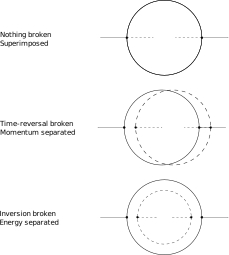
\includegraphics[width=0.75\textwidth]{figures/spinStructureWeyl}
  \caption{\label{fig:spinStructure} }
\end{figure}



\subsection{Symmetries}
In order to separate weyl cones in momentum, we introduce a pseuod spin degree of freedom, making the system 4x4.
We may then get solutions with the cones separated in momentum (or energy).
We may also ask what heppens if we try to separate tilted cones?

Firstly, in the most intuitive way to extend the 2x2 tilted cones to 4x4, we get that the cones tilt opposite direction, thus not superimposed even before separating in momentum.
They are after that simple to separate in momentum.
We might wonder if it makes sense to do it in this way.

The lattice model of the energy dispersion to explain tilted cones gives two cones separated in momentum, and tilting corresponds to ``bending'' the dispersion curves between them.
Maybe we therefore always have cones separated in momentum, and thus tilting superimposed does not make sense?
All depends on the origin of the tilt I believe.
Also, we must not confuse the global dispersion relation, to the Dirac cones which are expansions around the nodes.

Key to understand how spin behaves in all of this, and also maybe the symmetries.

To properly investigate the symmetry properties of the system, we must consider the 4x4, not 2x2 Hamiltonians.
While the 2x2 system does a goood job at describing a single cone, much important phsycis is lost when reducing the 4x4 Hamiltonian.
For example, the requirement that the total Berry curvature over the entire Briolluine zone is zero is not met for the 2x2 Hamiltonian, as it describes only one cone of a certain chirality.
The 4x4, however, includes two cones, which may in general be superimposed, thus conserving the total zero-divergence of the Berry curvature.
As a matter of fact, the inclusion of both cones is important also for symmetry considerations.

Let
\[
  H = v_{F} \tau _{x} \otimes \vec{\sigma} \vec{k},
\]
where \(\tau \) is some pseudo spin degree of freedom, transforming like \(\vec{r}\) under parity in time reversal.
This system describes two superimposed cones at the origin, with opposite chirality.
The effect of parity \(\mathcal{P}\) and time reversal \(\mathcal{T}\) is
\begin{table}[h]
  \centering
  \begin{tabular}{lcc}
    & \(\mathcal{P}\) & \(\mathcal{T}\)\\
    \hline
    \(\tau \) & - & +\\
    \(\sigma \) & + & -\\
    \(k\) & - & -
  \end{tabular}
\end{table}
\begin{equation}
  \label{eq:111}
  \begin{aligned}
    \mathcal{P} \tau \mathcal{P}^{\dagger} &= -\tau, & \mathcal{T} \tau \mathcal{T}^{\dagger} &= +\tau\\
    \mathcal{P} \sigma  \mathcal{P}^{\dagger} &= + \sigma,  & \mathcal{T} \sigma  \mathcal{T}^{\dagger} &= -\sigma \\
    \mathcal{P} k \mathcal{P}^{\dagger} &= -k, & \mathcal{T} k \mathcal{T}^{\dagger} &= -k
  \end{aligned}
\end{equation}
Obviously then, the Hamiltonian is both time reversal and parity invariant, as \(\mathcal{P} \mathcal{P}^{\dagger} = \mathcal{T} \mathcal{T}^{\dagger} = 1\).

A tilt term \(\tau _{x} \otimes \mathcal{I} \vec{\omega} _{0} \vec{k}\) breaks time reversal invariance, while maintaining parity invariance.
This is due to the two cones of opposite chirality tilting in opposite directions.

\begin{figure}[h]
  \centering
  \begin{tikzpicture}
    \draw[->] (-4, 0) -- (4, 0) node[right] {\(k\)};
    \draw[->] (0, 0) -- (0, 4) node[right] {\(E\)};

    % vf = 1, v0 = 0.8
    \draw[blue] (-3.5, 0.7) -- (0, 0) -- (2, 3.6) node[right] {\(\ket{\uparrow}\)} coordinate[pos=0.7] (a);
    \draw[red] (3.5, 0.7) node[right] {\(\ket{\downarrow }\)} -- (0, 0) -- (-2, 3.6)
    coordinate[pos=0.7] (b);

    \draw[->] (a) -- ++(1, 0);
    \draw[->] (b) -- ++(1, 0);
  \end{tikzpicture}
  \caption{Time reversal breaking in tilted system.
    Cross section in the tilt direction shown, with blue showing one cone and red the other.
    Black arrows indicate spin direction, which for \(\ket{\uparrow {}}\) is proporitional to  \(k\) while for \(\ket{\downarrow {}}\) is proportional to \( -k \).
  }
\end{figure}

The unperturbed Dirac Hamiltonian is Lorentz invariant, given that we consider an ``effective speed of light'', namely the Fermi velocity, instead of the actual speed of light \( c \).
Specifically, Lorentz invariance means invariance under the \emph{Lorentz group}.
The Lorentz group is the \( O(1,3) \) Lie group that conserves
\[
x_{\mu } x^{\mu } = t^2 - x^2 - y^2 - z^2,
\]
i.e. all isometries of Minkowski space.
More specifically, the group consists of all 3D rotations, \( O(3) \), and all \emph{boosts}.
A boost is a hyperbolic rotation from a spactial dimension to the temporal dimension.
If we now direct our focus at the Hamiltonian of the Dirac cone
\[
H = \pm v_{F} \vec{\sigma} \vec{p},
\]
we may easily show the Lorentz invariance of the system.
The time independent Schrodinger equation is
\begin{equation}
  \label{eq:112}
  H \ket{\psi } = E \ket{\psi } \implies (H^2 - E^2) \ket{\psi } = 0.
\end{equation}
As
\[
p^{\mu } = \left(\frac{E}{c}, \vec{p}\right),
\]
the operator in Eq. \eqref{eq:112} is nothing more than
\todo{ Make clear the matrix strucute here. There is an implicit identity matrix of size 2 }
\begin{equation}
  \label{eq:113}
  H^2-E^2 = v_{F}^2 \vec{p}^2 - c^2 \left(p^0\right)^2 ,
\end{equation}
where we used the anticommutation relation
\[
\{\sigma_{i}, \sigma_{j}\} =  2 \delta _{ij}
\]
of the Pauli matrices.
Using now the effective speed of light \( c=v_F \), Eq. \eqref{eq:113} is
\begin{equation}
  \label{eq:114}
  - v_F^2 p_{\mu } p^{\mu }.
\end{equation}
The invariance of \( x^{\mu} x_{\nu} \) is the very definition of the Lorentz group, and so is obviously Lorentz invariant.

Consider now a \emph{tilted} Dirac cone
\begin{equation}
  \label{eq:115}
  H = \pm v_F \vec{\sigma} \vec{p} + \omega_x k_x,
\end{equation}
where we, without loss of generality, chose the tilt to be in the \( x \)-direction.
By the same argumentation as above, the eigenequation
\[
  H \ket{\psi} = E\ket{\psi} \implies (H^2 - E^2)\ket{\psi} = 0
\]
leads to the equation
\begin{equation}
  \label{eq:116}
  -v_F^2 p^{\mu} p_{\mu} + \omega_{x} k_x (2 E - \omega_x k_x) = 0.
\end{equation}
This is \emph{not} invariant under a Lorentz transformation, as can be seen by, for example, a rotation around the \( z \)-axis.
\todo{Clean up p vs k}




\section{Conclusion and outlook}


\begin{description}
  \item[Tilt parallel to temperature gradient]
        -Time constraints did not compute for tilt parallel to \( \nabla T \).

  \item[The energy-momentum tensor]
        - Still open question

  \item[Fully covariant calculation]
        - Move the explicit tilt parameter in the lagrangian into the metric

  \item[Finite chemical potential and temperature]
        Similar to doen ine sec
\end{description}


\appendix
\chapter{Long expressions not included in the main text\label{cha:long_expression}}
\begin{lstlisting}[breaklines=true, caption={Expression for Type-II interband transition with \( t_z > 1 \), given in Mathematica format.\label{lst:typeii-interband-tzpos}},language=Mathematica]
(m/(-1 + tz^2) - (2*m*tz)/(-1 + tz^2) - (4*(-1 + m)*m*tz)/(-1 + tz^2) + (m*tz^2)/(-1 + tz^2) +
  tz*Sqrt[(m*tz^2*(1 + (-1 + m)*tz^2))/(-1 + tz^2)^2] + 2*(-1 + m)*tz*Sqrt[(m*tz^2*(1 + (-1 + m)*tz^2))/(-1 + tz^2)^2] -
  Sqrt[m + (-1 + m)*m*tz^2]/(-1 + tz^2) - (2*(-1 + m)*Sqrt[m + (-1 + m)*m*tz^2])/(-1 + tz^2) +
  (2*tz*Sqrt[m + (-1 + m)*m*tz^2])/(-1 + tz^2) + 2*(-1 + m)*Log[(1 - Sqrt[(1 + (-1 + m)*tz^2)/m])/(1 + tz)] +
  (-1 + m)*tz*Log[(1 - Sqrt[(1 + (-1 + m)*tz^2)/m])/(1 + tz)] -
  2*(-1 + m)^2*Log[((1 + tz)*Sqrt[m/(-1 + tz^2)])/(Sqrt[m/(-1 + tz^2)] - Sqrt[(1 + (-1 + m)*tz^2)/(-1 + tz^2)])] -
  (-2*(-1 + m)^(3/2)*Sqrt[-1 + m*tz^2] + (-1 + tz)*Sqrt[(-1 + m)*(-1 + m*tz^2)] -
    tz*(2*m^2 - (1 + tz)*(-1 + Sqrt[(-1 + m)*(-1 + m*tz^2)]) + m*(-3 + tz*(-1 + 2*Sqrt[(-1 + m)*(-1 + m*tz^2)]))) -
    (1 - m)*(-1 + tz)*(-1 + (1 + tz)*(2 + tz)*Log[-((-1 + tz)*Sqrt[(-1 + m)/(-1 + tz^2)])]) -
    (-1 + tz^2)*(-2 + m*(2 + tz))*Log[(Sqrt[-1 + m] + Sqrt[-1 + m*tz^2])/Sqrt[-1 + tz^2]] +
    tz*Log[(-(Sqrt[-1 + m]*tz) + Sqrt[-1 + m*tz^2])/Sqrt[-1 + tz^2]] -
    tz^3*Log[(-(Sqrt[-1 + m]*tz) + Sqrt[-1 + m*tz^2])/Sqrt[-1 + tz^2]] -
    2*(-1 + m)^2*(tz + (-1 + tz^2)*Log[(-1 + m + Sqrt[(-1 + m)*(-1 + m*tz^2)])/(-1 + m + tz - m*tz)]))/(-1 + tz^2) -
  tz*Log[(m*tz - Sqrt[m + (-1 + m)*m*tz^2])/(-1 + tz)])/4
\end{lstlisting}


\begin{lstlisting}[breaklines=true, caption={Expression for Type-II interband transition with \( t_z < -1 \), given in Mathematica format.\label{lst:typeii-interband-tzneg}},language=Mathematica]
(1 + Sqrt[(-1 + m)*(-1 + m*tz^2)] - 2*m*Sqrt[(-1 + m)*(-1 + m*tz^2)] - Sqrt[m + (-1 + m)*m*tz^2] +
  2*m*Sqrt[m + (-1 + m)*m*tz^2] + (-1 + m)*(2 + tz)*Log[-((1 + tz)*Sqrt[(-1 + m)/(-1 + tz^2)])] +
  (-2 + m*(2 + tz))*Log[-((-1 + tz)*Sqrt[m/(-1 + tz^2)])] + 2*Log[(Sqrt[m]*(1 - tz))/(Sqrt[m] + Sqrt[1 + (-1 + m)*tz^2])] -
  4*m*Log[(Sqrt[m]*(1 - tz))/(Sqrt[m] + Sqrt[1 + (-1 + m)*tz^2])] +
  2*m^2*Log[(Sqrt[m]*(1 - tz))/(Sqrt[m] + Sqrt[1 + (-1 + m)*tz^2])] +
  2*Log[(Sqrt[m] + Sqrt[1 + (-1 + m)*tz^2])/Sqrt[-1 + tz^2]] - 2*m*Log[(Sqrt[m] + Sqrt[1 + (-1 + m)*tz^2])/Sqrt[-1 + tz^2]] +
  tz*Log[(Sqrt[m] + Sqrt[1 + (-1 + m)*tz^2])/Sqrt[-1 + tz^2]] - m*tz*Log[(Sqrt[m] + Sqrt[1 + (-1 + m)*tz^2])/Sqrt[-1 + tz^2]] +
  tz*Log[(-(Sqrt[m]*tz) + Sqrt[1 + (-1 + m)*tz^2])/Sqrt[-1 + tz^2]] -
  tz*Log[(-(Sqrt[-1 + m]*tz) + Sqrt[-1 + m*tz^2])/Sqrt[-1 + tz^2]] - 2*Log[(1 - Sqrt[(-1 + m*tz^2)/(-1 + m)])/(1 + tz)] +
  4*m*Log[(1 - Sqrt[(-1 + m*tz^2)/(-1 + m)])/(1 + tz)] - 2*m^2*Log[(1 - Sqrt[(-1 + m*tz^2)/(-1 + m)])/(1 + tz)] +
  2*Log[-Sqrt[(-1 + m)/(-1 + tz^2)] + Sqrt[(-1 + m*tz^2)/(-1 + tz^2)]] -
  2*m*Log[-Sqrt[(-1 + m)/(-1 + tz^2)] + Sqrt[(-1 + m*tz^2)/(-1 + tz^2)]] -
  m*tz*Log[-Sqrt[(-1 + m)/(-1 + tz^2)] + Sqrt[(-1 + m*tz^2)/(-1 + tz^2)]])/4
\end{lstlisting}

\begin{lstlisting}[breaklines=true, caption={Expression for Type-II intraband transition with \( t_z > 1 \), given in Mathematica format.\label{lst:typeii-intraband-tzpos}},language=Mathematica]
(-((-1 + m)*m*tz*AppellF1[1, 1/2, 1/2, 2, (1 - tz^2)^(-1), (1 - m)/(m*(-1 + tz^2))]) +
  m^2*tz*AppellF1[1, 1/2, 1/2, 2, -(m/((-1 + m)*(-1 + tz^2))), (1 - tz^2)^(-1)] +
  (-1 + tz^2)*(-2*Sqrt[(-1 + m)*m^3] + 2*m^2*Sqrt[(-1 + m)*(1 + (-1 + m)*tz^2)] - 4*m^3*Sqrt[(-1 + m)*(1 + (-1 + m)*tz^2)] +
    2*Sqrt[m^3*(-1 + m*tz^2)] - 6*Sqrt[m^5*(-1 + m*tz^2)] + 4*Sqrt[m^7*(-1 + m*tz^2)] -
    (-2*Sqrt[(-1 + m)*m^5] + 2*Sqrt[(-1 + m)*m^7] + (-Sqrt[(-1 + m)*m^3] + Sqrt[(-1 + m)*m^5])*tz)*Log[-1 + m] -
    2*Sqrt[(-1 + m)*m^5]*Log[m] + 2*Sqrt[(-1 + m)*m^7]*Log[m] + Sqrt[(-1 + m)*m^5]*tz*Log[m] +
    2*Sqrt[(-1 + m)*m^3]*tz*Log[1 + tz] - Sqrt[(-1 + m)*m^3]*tz*Log[-1 + tz^2] -
    4*Sqrt[(-1 + m)*m^5]*Log[(Sqrt[m] + Sqrt[1 + (-1 + m)*tz^2])/Sqrt[-1 + tz^2]] +
    4*Sqrt[(-1 + m)*m^7]*Log[(Sqrt[m] + Sqrt[1 + (-1 + m)*tz^2])/Sqrt[-1 + tz^2]] -
    2*Sqrt[(-1 + m)*m^3]*tz*Log[(Sqrt[m] + Sqrt[1 + (-1 + m)*tz^2])/Sqrt[-1 + tz^2]] +
    2*Sqrt[(-1 + m)*m^5]*tz*Log[(Sqrt[m] + Sqrt[1 + (-1 + m)*tz^2])/Sqrt[-1 + tz^2]] +
    4*Sqrt[(-1 + m)*m^5]*Log[(Sqrt[-1 + m] + Sqrt[-1 + m*tz^2])/Sqrt[-1 + tz^2]] -
    4*Sqrt[(-1 + m)*m^7]*Log[(Sqrt[-1 + m] + Sqrt[-1 + m*tz^2])/Sqrt[-1 + tz^2]] -
    2*Sqrt[(-1 + m)*m^5]*tz*Log[(Sqrt[-1 + m] + Sqrt[-1 + m*tz^2])/Sqrt[-1 + tz^2]]))/(8*Sqrt[-1 + m]*m^(3/2)*(-1 + tz^2))
\end{lstlisting}

\begin{lstlisting}[breaklines=true, caption={Expression for Type-II intraband transition with \( t_z < - 1 \), given in Mathematica format.\label{lst:typeii-intraband-tzneg}},language=Mathematica]
(4*m*(-1 + tz)*Sqrt[(-1 + m)*(1 + (-1 + m)*tz^2)]*(-1 + Abs[tz]) - 4*(-1 + m)*(-1 + tz)*Sqrt[m*(-1 + m*tz^2)]*(-1 + Abs[tz]) +
  8*(-1 + m)^(3/2)*m*Sqrt[1 + (-1 + m)*tz^2]*(1 + tz*Abs[tz]) - 8*(-1 + m)^2*Sqrt[m*(-1 + m*tz^2)]*(1 + tz*Abs[tz]) +
  2*(-1 + m)*tz*(AppellF1[1, 1/2, 1/2, 2, (1 - tz^2)^(-1), (1 - m)/(m*(-1 + tz^2))] -
    AppellF1[1, 1/2, 1/2, 2, m/(-1 + m - (-1 + m)*tz^2), (1 - tz^2)^(-1)]) -
  2*tz*AppellF1[1, 1/2, 1/2, 2, m/(-1 + m - (-1 + m)*tz^2), (1 - tz^2)^(-1)] -
  4*(-1 + m)^(5/2)*Sqrt[m]*(-1 + tz^2)*(Log[(-1 + m)/m] - 2*Log[(Sqrt[m] + Sqrt[1 + (-1 + m)*tz^2])/Sqrt[-1 + tz^2]] +
    2*Log[(Sqrt[-1 + m] + Sqrt[-1 + m*tz^2])/Sqrt[-1 + tz^2]]) - Sqrt[(-1 + m)*m]*(-1 + tz)*
   (-4 + 4*Abs[tz] + tz*Log[m/(-1 + tz^2)] + 4*tz*Log[(Sqrt[-1 + m] + Sqrt[-1 + m*tz^2])/Sqrt[-1 + tz^2]] +
    4*tz^2*Log[(Sqrt[-1 + m] + Sqrt[-1 + m*tz^2])/Sqrt[-1 + tz^2]] + 2*tz*Log[1 + Abs[tz]] -
    6*tz*Log[Sqrt[m/(-1 + tz^2)]*(1 + Abs[tz])] - 4*tz^2*Log[Sqrt[m/(-1 + tz^2)]*(1 + Abs[tz])]) +
  (-1 + m)^(3/2)*Sqrt[m]*(8*tz + 8*Abs[tz] + Log[(-1 + m)/m] - tz^2*Log[(-1 + m)/(-1 + tz^2)] + tz^2*Log[m/(-1 + tz^2)] -
    8*Log[(Sqrt[m] + Sqrt[1 + (-1 + m)*tz^2])/Sqrt[-1 + tz^2]] - 4*tz*Log[(Sqrt[m] + Sqrt[1 + (-1 + m)*tz^2])/Sqrt[-1 + tz^2]] +
    8*tz^2*Log[(Sqrt[m] + Sqrt[1 + (-1 + m)*tz^2])/Sqrt[-1 + tz^2]] +
    4*tz^3*Log[(Sqrt[m] + Sqrt[1 + (-1 + m)*tz^2])/Sqrt[-1 + tz^2]] +
    8*Log[(Sqrt[-1 + m] + Sqrt[-1 + m*tz^2])/Sqrt[-1 + tz^2]] + 4*tz*Log[(Sqrt[-1 + m] + Sqrt[-1 + m*tz^2])/Sqrt[-1 + tz^2]] -
    8*tz^2*Log[(Sqrt[-1 + m] + Sqrt[-1 + m*tz^2])/Sqrt[-1 + tz^2]] -
    4*tz^3*Log[(Sqrt[-1 + m] + Sqrt[-1 + m*tz^2])/Sqrt[-1 + tz^2]] + 6*Log[Sqrt[(-1 + m)/(-1 + tz^2)]*(1 + Abs[tz])] +
    4*tz*Log[Sqrt[(-1 + m)/(-1 + tz^2)]*(1 + Abs[tz])] - 6*tz^2*Log[Sqrt[(-1 + m)/(-1 + tz^2)]*(1 + Abs[tz])] -
    4*tz^3*Log[Sqrt[(-1 + m)/(-1 + tz^2)]*(1 + Abs[tz])] - 6*Log[Sqrt[m/(-1 + tz^2)]*(1 + Abs[tz])] -
    4*tz*Log[Sqrt[m/(-1 + tz^2)]*(1 + Abs[tz])] + 6*tz^2*Log[Sqrt[m/(-1 + tz^2)]*(1 + Abs[tz])] +
    4*tz^3*Log[Sqrt[m/(-1 + tz^2)]*(1 + Abs[tz])]))/(16*Sqrt[(-1 + m)*m]*(-1 + tz^2))
\end{lstlisting}


% \begin{multline}
%   \label{eq:typeii-interband-tzpos}
%   \frac{1}{4} \Bigg\{
%   -\frac{1}{t_z^2-1}
%   \Bigg[
%   t_z \left(2 m^2+m \left(t_z \left(2 \sqrt{(m-1) \left(m t_z^2-1\right)}-1\right)-3\right)\\
%     -(t_z+1) \left(\sqrt{(m-1) \left(m t_z^2-1\right)}-1\right)\right)-2 (m-1)^{3/2} \sqrt{m t_z^2-1}+(t_z-1) \sqrt{(m-1) \left(m
%       t_z^2-1\right)}\\
%   +t_z \log \left(t_z \sqrt{\frac{m-1}{t_z^2-1}}+\sqrt{\frac{m t_z^2-1}{t_z^2-1}}\right)-(1-m) (t_z-1) \left[\left(t_z^2+3 t_z+2\right) \log \left((t_z+1)
%       \sqrt{\frac{m-1}{t_z^2-1}}\right)
%     -1\right]\\
%   -\left(t_z^2-1\right) (m (t_z+2)-2) \log \left(\frac{\sqrt{m t_z^2-1}+\sqrt{m-1}}{\sqrt{t_z^2-1}}\right)\\
%   -2 (m-1)^2 \left(\left(t_z^2-1\right) \log \left(\frac{\sqrt{(m-1) \left(m
%             t_z^2-1\right)}+m-1}{(m-1) (t_z+1)}\right)+t_z\right)\\
%   +t_z^3 \left(-\log \left(t_z \sqrt{\frac{m-1}{t_z^2-1}}+\sqrt{\frac{m t_z^2-1}{t_z^2-1}}\right)\right)
%   \Bigg]
%   +\frac{2 (m-1) t_z^2 \sqrt{(m-1) m
%       t_z^2+m}}{t_z^2-1}\\
%   -\frac{2 (m-1) \sqrt{(m-1) m t_z^2+m}}{t_z^2-1}+\frac{t_z^2 \sqrt{(m-1) m t_z^2+m}}{t_z^2-1}-\frac{\sqrt{(m-1) m t_z^2+m}}{t_z^2-1}+\frac{m t_z^2}{1-t_z^2}\\
%   +\frac{m}{t_z^2-1}-2 (m-1)^2 \log
%   \left(-\frac{(t_z-1) \sqrt{\frac{m}{t_z^2-1}}}{\sqrt{\frac{m}{t_z^2-1}}-\sqrt{\frac{(m-1) t_z^2+1}{t_z^2-1}}}\right)-(m-1) t_z \log \left((t_z-1) \sqrt{\frac{m}{t_z^2-1}}\right)\\
%   -2 (m-1) \log \left((t_z-1)
%     \sqrt{\frac{m}{t_z^2-1}}\right)+(m-1) t_z \log \left(\sqrt{\frac{(m-1) t_z^2+1}{t_z^2-1}}-\sqrt{\frac{m}{t_z^2-1}}\right)\\
%   +2 (m-1) \log \left(\sqrt{\frac{(m-1) t_z^2+1}{t_z^2-1}}-\sqrt{\frac{m}{t_z^2-1}}\right)-t_z \log
%   \left((t_z-1) \sqrt{\frac{m}{t_z^2-1}}\right)\\
%   -t_z \log \left(t_z \sqrt{\frac{m}{t_z^2-1}}+\sqrt{\frac{(m-1) t_z^2+1}{t_z^2-1}}\right)
%   \Bigg\}
% \end{multline}

\begin{multline}
  \label{eq:typeii-interband-tzneg}
\end{multline}

\begin{multline}
  \label{eq:typeii-intraband-tzpos}
\end{multline}


\begin{multline}
  \label{eq:typeii-intraband-tzneg}
\end{multline}

\chapter{Contributions from the Symmetric Energy-Momentum Tensor}\label{sec:otherterm-appendix}
As noted in the main text, there are some subtlety in the definition of the energy-momentum tensor.
The \emph{canonical} definition, which we have used in the main text, is in general not symmetric.
% The tensor enter our calculation from the conservation law
% \[
% \partial_\mu T^{\mu \nu} = 0,
% \]
% which for \( \nu = 0 \) is nothing more than the conservation law of energy: \( \partial_t \epsilon - \vec{\nabla} \vec{J}_\epsilon = 0 \), where \( \epsilon \) is energy density and \( \vec{J}_\epsilon \) is the energy current.
In the calculation by~\textcite{arjonaFingerprintsConformalAnomaly2019}, the symmetrized\footnote{See \cref{sec:commen-T} for a more precise discussion on the symmetrization of the energy-momentum tensor.}
energy-momentum tensor
\[
T_S^{\mu \nu} = \frac{T^{\mu \nu} + T^{\nu \mu}}{2}
\]
was used.
In this appendix we show the contributions of the symmetric tensor.
The contributions from \( T^{\mu \nu} \) and \( T^{\nu \mu} \) are shown to be equal in the non-tilted case, while they differ in the tilted case.

In the main text we have already found the contributions from the canonical tensor, and so we focus here on the contributions from \( T_F^{\mu \nu } = T^{\nu \mu} \).
The relevant element is \( T_F^{y 0} = T^{0 y} \).

The tilted canonical energy-momentum tensor, \cref{eq:T-canon-tilt},
\[
  T^{\mu\nu} =
  \frac{i}{2} (
  \phi^{\dagger} \tilde{\sigma}_s ^{\mu} \partial_{\nu} \phi
  - \partial_{\nu} \phi^{\dagger} \tilde{\sigma}_s ^{\mu} \phi
  - \eta^{\mu \nu} \mathcal{L}
  ),
\]
and so the symmetric tensor is
\renewcommand\overleftrightarrow[1]{\overset{\tiny\leftrightarrow}{#1}}
\begin{equation}
  \label{eq:87}
  T_S^{\mu\nu} =
  \frac{i}{2} (
  \phi^{\dagger} \tilde{\sigma}_s ^{\mu} \overleftrightarrow{\partial}_{\nu} \phi
  +
  \phi^{\dagger} \tilde{\sigma}_s ^{\nu} \overleftrightarrow{\partial}_{\mu} \phi
  - \eta^{\mu \nu} \mathcal{L}
  ),
\end{equation}
where we used the notation \( \phi^{\dagger} \overleftrightarrow{\partial} \phi = (\phi^{\dagger} \partial \phi - (\partial \phi^{\dagger}) \phi) /2 \).
We split \( T_S^{y0} \) into three parts;
the first part corresponds to the canonical energy-momentum tensor, while the two latter correspond to the two terms of \( T_F^{y0} \).
Explicitly
\begin{equation}
  \label{eq:88}
  T_S^{y 0} =
  \underbrace{\frac{i}{2} \phi^{\dagger} \tilde{\sigma}_s^{y} \overleftrightarrow{\partial_0} \phi}_{T^{(1)}}
  +  \underbrace{ \frac{i}{4} \phi^{\dagger} \partial_y \phi}_{T^{(2)}}
  + \underbrace{ \frac{i}{4} \phi^{\dagger} \partial_y \phi}_{T^{(3)}}.
\end{equation}
In other words, the first part is half that found in the main text, while the two latter are unique to the symmetric tensor.
For convenience, we will for the rest of the appendix rename \( T^{\mu \nu} = T_S^{\mu \nu} \).

\section{No tilt}\label{sec:otherstressterm:notilt}
Begin by considering the matrix elements
\begin{align}
  \label{eq:144}
  T ^{0y\; (2)} _{\vec{k}+\qvec{q}ns, \vec{k}ms} (\vec{q}) &= +
                                                            \frac{1}{4}
                                                            \int \mathrm{d}y
                                                            e^{iq_y y} v_F
                                                            \phi ^{*}_{\vec{k}+\qvec{q} ns}(y)
                                                            p_y \phi _{\vec{k}ms} (y),\\
  \label{eq:145}
  T ^{0y\; (3)} _{\vec{k}+\qvec{q}ns, \vec{k}ms} (\vec{q}) &= -
                                                            \frac{1}{4}
                                                            \int \mathrm{d}y
                                                            e^{iq_y y} v_F
                                                            \left( p_y\phi ^{*}_{\vec{k}+\qvec{q} ns}(y) \right)
                                                            \phi _{\vec{k}ms}(y).
\end{align}
Recall that $\phi_{\vec{k}ms} (y)$, defined in \cref{eq:72}, consists of two $y$-dependent factors:
\(
  \exp \left[-\frac{(y-k_x l_B^2)^2}{2 l_{B}^2 } \right]
\)
and the Hermite polynomials.
The operator $p_y$ thus produces two terms when operating on $\phi $.
The first term, coming from the exponent, is proportional to $y-k_xl_B^2$.
The operator in \cref{eq:144,eq:145} acts on $\phi $ with the quantum  number $\vec{k}$ and $\vec{k} + \qvec{q}$, respectively;
when summing the two contributions, everything thus cancels except for a term proportional to $q_x$, which vanishes in the local limit.

It remains to consider the result of $p_y$ operating on the Hermite polynomials.
Let $\tilde{p}_y$ indicate the $p_y$ operator acting only on the Hermite polynomial part of $\phi $, and use the property of Hermite polynomials $\partial _x H_n(x) = 2 n H_{n-1}(x)$~\cite[Eq.~18.9.25]{NIST:DLMF}.
\begin{multline}
      \phi ^{*}_{\vec{k}+\qvec{q}ns}(y) \tilde{p}_y \phi _{\vec{k}ms} =
    -i \hbar \exp \left\{
      - \frac{(y-k_xl_B^2)^2 + (y-(k_x + q_x) l_B^2)^2}{2 l_B^2}
    \right\}\\
    \frac{2}{l_B}\Bigg\{
      (M-1) a _{\vec{k} ms}a _{\vec{k}+\qvec{q} ns} H_{M-2}\left( \frac{y-k_x l_B^2}{l_B} \right) H_{N-1} \left( \frac{y - (k_x+q_x)l_B^2}{l_B} \right)\\
      + M b _{\vec{k} ms} b _{\vec{k}+\qvec{q} ns} H_{M-1} \left( \frac{y - k_xl_B^2}{l_B} \right) H_N \left( \frac{y - (k_x+q_x)l_B^2}{l_B} \right)
    \Bigg\}.
\end{multline}
Completing the square, we get
\begin{multline}
  \int \mathrm{d}y e^{iq_y y} \phi ^{*}_{\vec{k}+\qvec{q} ns}(y) \tilde{p}_y \phi _{\vec{k} ms}(y) =
  -i\hbar
  \exp \left[ -\frac{l_B^2}{4} \left\{ \qvec{q}_y^2 - 2iq_y ( 2k_x + q_x) \right\} \right]\\
  \int \mathrm{d}y
  \exp \left[
    - \left\{
      y + \frac{l_B^2}{2} \left( -iq_y - 2k_x - q_x \right)
    \right\} ^2
    / l_B^2
  \right]\\
  \frac{2}{l_B}\Bigg\{
  (M-1) a _{\vec{k}ms}a _{\vec{k}+\qvec{q} ns} H_{M-2}\left( \frac{y-k_x l_B^2}{l_B} \right) H_{N-1} \left( \frac{y - (k_x+q_x)l_B^2}{l_B} \right)\\
  + M b _{\vec{k} ms} b _{\vec{k}+\qvec{q} ns} H_{M-1} \left( \frac{y - k_xl_B^2}{l_B} \right) H_N \left( \frac{y - (k_x+q_x)l_B^2}{l_B} \right)
  \Bigg\}.
\end{multline}
Upon introducing $\tilde{y} = \frac{y}{l_B} + l_B( -iq_y - q_x - 2k_x) / 2$, as was also done in the main text, the expression reduces to
\begin{multline}
  \int \mathrm{d}y e^{iq_y y} \phi ^{*}_{\vec{k}+\qvec{q} ns}(y) \tilde{p}_y \phi _{\vec{k} ms}(y) =
  -i\hbar
  \exp \left[ -\frac{l_B^2}{4} \left\{ q_x^2 + q_y^2 - 2iq_y ( 2k_x + q_x) \right\} \right]\\
  \int \mathrm{d}\tilde{y} l_B
  \exp \left[
    - \tilde{y}^2
  \right]\\
  \frac{2}{l_B}\Bigg\{
  (M-1) a _{\vec{k}ms}a _{\vec{k}+\qvec{q} ns}
  H_{M-2}\left( \tilde{y} + \frac{l_B}{2}(iq_y + q_x) \right)
  H_{N-1} \left( \tilde{y} + \frac{l_B}{2}(iq_y - q_x) \right)\\
  + M b _{\vec{k} ms} b _{\vec{k}+\qvec{q} ns}
  H_{M-1} \left( \tilde{y} + \frac{l_B}{2}(iq_y + q_x)\right)
  H_N \left( \tilde{y} + \frac{l_B}{2}(iq_y - q_x) \right)
  \Bigg\}.
\end{multline}

Considering now the local limit \( \vec{q} \to 0 \), the expression greatly simplifies, and we may use the orthogonality relation for the Hermite polynomials \cref{eq:hermite-ortho}
\[
  \int\limits_{-\infty}^{\infty} \mathrm{d}x e^{-x^2} H_n(x)H_m(x) = \sqrt{\pi} 2^{n} n! \delta_{n,m}
\]
to evaulate the integral.
\begin{equation}
  \label{eq:146}
  \lim_{\vec{q} \to 0} \int \mathrm{d}y e^{iq_y y} \phi ^{*}_{\vec{k}+\qvec{q} ns}(y) \tilde{p}_y \phi _{\vec{k} ms}(y) =
  -i \hbar \sqrt{2}
  \frac{
    \alpha_{k m s} \alpha_{k n s} \sqrt{M-1}
    +
    \sqrt{M}
  }{
    {l_{B} \sqrt{\alpha_{k m s}^2 + 1}\sqrt{\alpha_{k n s} ^2 + 1}}
  }
  \delta_{N, M-1}.
\end{equation}

Similarly, for $T^{0y\; (3)}_{\vec{k}+\qvec{q}ns, \vec{k}ms} (\vec{q})$, one has
\begin{multline}
  \left( \tilde{p}_y \phi ^{*}_{\vec{k}+\qvec{q} ns}(y) \right)
  \phi _{\vec{k} m s}(y) =
  -i \hbar \exp \left\{
    - \frac{(y-k_xl_B^2)^2 + (y-(k_x + q_x) l_B^2)^2}{2 l_B^2}
  \right\}\\
  \frac{2}{l_{B}} \left\{
    (N-1) a_{\vec{k} m s} a_{\vec{k} + \qvec{q} n s} H_{M-1} \left( \frac{y-k_xl_B^2}{l_B} \right)H_{N-2} \left( \frac{y - (k_x + q_x) l_B^2}{l_B} \right) \right.\\
  \left. +
    N b_{\vec{k} m s} b_{\vec{k}+\qvec{q} n s} H_M \left( \frac{y - k_xl_B^2}{l_B} \right) H_{N-1}\left( \frac{y-(k_x+q_x) l_B^2}{l_B} \right)
  \right\}
\end{multline}
which with the same procedure as above gives
\begin{equation}
 \lim_{\vec{q}\to 0} \int \mathrm{d}y e^{iq_y y}
  \left( \tilde{p}_y \phi ^{*}_{\vec{k}+\qvec{q} ns}(y) \right)
  \phi _{\vec{k} m s}(y)
  =
  -i \hbar \sqrt{2}
  \frac{
    \alpha_{k m s} \alpha_{k n s} \sqrt{N-1}
    +
    \sqrt{N}
  }{
    {l_{B} \sqrt{\alpha_{k m s}^2 + 1}\sqrt{\alpha_{k n s} ^2 + 1}}
  }
  \delta_{M, N-1}.
\end{equation}

\begin{summary}\label{summary:notilt-otherterm}%
  In the untilted case, we have
  \begin{align}
    \label{eq:71}
    \lim_{\vec{q} \to 0} T^{y0\; (2)}_{\vec{k} n s, \vec{k} m s} &= -\frac{i \hbar \sqrt{2}}{4}
        \frac{
          \alpha_{k m s} \alpha_{k n s} \sqrt{M-1}
          +
          \sqrt{M}
        }{
          {l_{B} \sqrt{\alpha_{k m s}^2 + 1}\sqrt{\alpha_{k n s} ^2 + 1}}
        }
                                                                   \delta_{N, M-1},\\
    \lim_{\vec{q} \to 0} T^{y0\; (3)}_{\vec{k} n s, \vec{k} m s} &= \frac{i \hbar \sqrt{2}}{4}
        \frac{
          \alpha_{k m s} \alpha_{k n s} \sqrt{N-1}
          +
          \sqrt{N}
        }{
          {l_{B} \sqrt{\alpha_{k m s}^2 + 1}\sqrt{\alpha_{k n s} ^2 + 1}}
        }
                                                                   \delta_{M, N-1}.
  \end{align}
\end{summary}

\section{With tilt}
In the tilted case, we have shown in the main text that \todo{insert ref}
\[
  T^{\mu 0} = \frac{i}{2}
  \left[\partial_i \bar{\psi} \Gamma^j \gamma^0 \Gamma^{\mu} \psi
    - \bar{\psi} \Gamma^{\mu} \gamma^0 \Gamma^j \partial_j \psi
  \right].
\]
Swapping the indices, we have for \( \mu \neq 0 \)~\cite{vanderwurffMagnetovorticalThermoelectricTransport2019}
\[
  T^{0 i} = \frac{i}{2} [\bar{\psi} \gamma^0 \partial^{\mu } \psi
  - \partial^{\mu }\bar{\psi} \gamma^{0 } \psi ].
\]
In our work, we have considered only tilt perpendiculat to the thermal gradient,  so the component of the energy-momentum tensor of interest are not affected by the tilt.

or
\begin{align}
  T_{\vec{k} + \qvec{q} ns, \vec{k} ms}^{0y (2)} (\vec{q}) &=
                                                             + \frac{1}{4} \int \mathrm{d} y
                                                             e^{iq_{y} y} v_{F}
                                                             \phi ^{*}_{\vec{k}+\qvec{q} ns} (y) p_{y} \phi _{\vec{k} m s} (y),\\
  T_{\vec{k} + \qvec{q} ns, \vec{k} ms}^{0y (3)} (\vec{q}) &=
                                                             - \frac{1}{4} \int \mathrm{d} y
                                                             e^{iq_{y} y} v_{F}
                                                             (p_{y} \phi ^{*}_{\vec{k}+\qvec{q} ns} (y))  \phi _{\vec{k} m s} (y).
\end{align}
Firstly, we note that
\[
  [p_{y} , e^{\theta /2 \sigma _{x}}] = 0.
\]
Furthermore, exactly as for the untilted case, the momentum operator acting on the exponential prefactor of \(\phi \) gives contributions proportional to \(q_{x}\).
In the local limit \(q\to  0\) this term vanishes, and we need only consider the effect of the momentum operator acting on the Hermite polynomials.

Denote by \(\tilde{p}_{y}\) the momentum operator \(p_{y}\) acting only on the Hermite polynomial part of \(\phi \).
Furthermore, we will use the property of Hermite polynomials \(\partial _{x} H_{n} (x) = 2 n H_{n-1} (x)\)~\cite[Eq.~18.9.25]{NIST:DLMF}.
\begin{align}
  \tilde{p}_{y} \phi _{\vec{k} ms} &=
  -i \hbar
  e^{\theta /2 \sigma _{x}}
  e^{-\frac{1}{2} \chi ^2}
  \partial _{y}
  \begin{pmatrix}
    a_{\vec{k} m s} H_{M-1} (\chi) \\
    b_{\vec{k} ms} H_{M} (\chi)
  \end{pmatrix}\\
                                   &=
                                     -i \hbar
                                     e^{\theta /2 \sigma _{x}}
                                     e^{-\frac{1}{2} \chi ^2}
                                     2 \frac{\partial \chi }{\partial y}
                                     \begin{pmatrix}
                                       a_{\vec{k} m s} (M-1) H_{M-2} (\chi) \\
                                       b_{\vec{k} ms} (M) H_{M-1} (\chi)
                                     \end{pmatrix}\\
                                   &=
                                     -i \hbar
                                     e^{\theta /2 \sigma _{x}}
                                     e^{-\frac{1}{2} \chi ^2}
                                     \frac{2 \sqrt{\alpha}}{ l_{B} }
                                     \begin{pmatrix}
                                       a_{\vec{k} m s} (M-1) H_{M-2} (\chi) \\
                                       b_{\vec{k} ms} (M) H_{M-1} (\chi)
                                     \end{pmatrix}.
\end{align}
And thus, recalling that
\[
  e^{\theta \sigma _{x}} =
  \begin{pmatrix}
    1 & -t_{x}\\
    -t_{x} & 1
  \end{pmatrix}
  \frac{1}{\sqrt{1-t_{x}^2}},
\]
we find the product
\begin{multline}
  \phi ^{*} _{\vec{k} + \qvec{q} ns} (y) \tilde{p}_{y} \phi _{\vec{k} m s}
  % = -\frac{i\hbar 2 \sqrt{\alpha } }{ l_{B} }
  % e^{-\frac{1}{2} \chi _{\vec{k}}^2 - \frac{1}{2} \chi _{\vec{k} + \qvec{q}} ^2}
  % \phi ^{*}_{\vec{k} + \qvec{q} ns}(y)
  % e^{\theta \sigma _{x}}
  % \phi _{\vec{k} ms} (y)\\
  % %
  = -\frac{i\hbar 2 \sqrt{\alpha } }{l_{B} \sqrt{1 - t_{x}^2} }
  e^{-\frac{1}{2} \chi _{\vec{k}}^2 - \frac{1}{2} \chi _{\vec{k} + \qvec{q}} ^2}\\
  \Big[
  a_{\vec{k} + \qvec{q} ns} H_{N-1}(\chi_{\vec{k}+\qvec{q}})
  \left\{a_{\vec{k} ms} (M-1) H_{M-2} (\chi_{\vec{k}}) - t_{x} b_{\vec{k} ms} M H_{M-1} (\chi_{\vec{k}})\right\}\\
  +
  b_{\vec{k} + \qvec{q} ns} H_{N} (\chi_{\vec{k} + \qvec{q}})
  \left\{-t_{x} a_{\vec{k} ms} (M-1) H_{M-2} (\chi_{\vec{k}}) + b_{\vec{k} ms} M H_{M-1} (\chi_{\vec{k}})\right\}
  \Big].
\end{multline}
Completing the square and substituting
\[
  \tilde{y} = \frac{\sqrt{ \alpha  }}{l_{B}}
  \left(y - \frac{l_{B}^2}{2 \alpha } (i q_{y} + (2 k'_x + q' _x) ) \right)
\]
gives
\begin{multline}
  \int \mathrm{d}y
  e^{i q_{y}}
  \phi ^{*}_{\vec{k} + \qvec{q} ns}(y) \tilde{p}_{y}
  \phi_{\vec{k} ms} (y)
  =
  \exp
  \left[
    - \frac{l_{B}^2}{4 \alpha } (q_{y}^2 - 2 i (2k' _x + q' _x) q_{y} + (q' _x)^2 )
  \right  ]\\
\times\frac{ - i\hbar 2 \sqrt{\alpha} }{l_{B} \sqrt{1 - t_{x}^2} }
  \int \mathrm{d} \tilde{y} \frac{l_{B}}{\sqrt{\alpha } }\\
\times  \Big[
  a_{\vec{k} + \qvec{q} ns} H_{N-1}( \chi _{\vec{k} + \qvec{q}} )
  \left\{
    a_{\vec{k} ms} (M-1) H_{M-2} ( \chi _{\vec{k}} )
    - t_{x} b_{\vec{k} ms} M H_{M-1} ( \chi _{\vec{k}} ) \right\}\\
  +
  b_{\vec{k} + \qvec{q} ns} H_{N} ( \chi _{\vec{k} + \qvec{q}} )
  \left\{
    -t_{x} a_{\vec{k} ms} (M-1) H_{M-2} ( \chi _{\vec{k}} )
    + b_{\vec{k} ms} M H_{M-1} ( \chi _{\vec{k}} )
  \right\}
  \Big].
\end{multline}

We must now evaluate the integral, and express the result in the \( \Xi \)-functions, defined in \cref{eq:xi1def,eq:xi2def} of the main text.
\[
    \begin{pmatrix}
      a_{\vec{k} + \qvec{q} n s} H_{N-1} ( \chi _{\vec{k} + \qvec{q}} )\\
      b_{\vec{k} + \qvec{q} ns} H_N ( \chi _{\vec{k} + \qvec{q}} )
    \end{pmatrix}^{T}
  \underbrace{
    \begin{pmatrix}
      1 & -t_x\\
      -t_x & 1
    \end{pmatrix}
    }_{T}
    \begin{pmatrix}
      a_{\vec{k} m s} (M-1) H_{M-2} (\chi_{\vec{k}})\\
      b_{\vec{k} m s} M H_{M-1} ( \chi _{\vec{k}} )
    \end{pmatrix}
\]
For each of the entries in \( T \), we get a product of Hermite polynomials.
Where the untilted cone had two such terms, the tilt parameter \( t _x \) now gives two extra products, which we must evaluate.
Let \( M^{(2)}_{ij} \) be the product corresponding to \( T_{ij} \), i.e.
\begin{align}
  M^{(2)}_{11} &= \phantom{-t_x} a_{\vec{k} + \qvec{q} ns} a_{\vec{k} ms} (M-1) H_{N-1} (\chi_{\vec{k} + \qvec{q}}) H_{M-2} (\chi_{\vec{k}}),\\
  M^{(2)}_{12} &= -t_x a_{\vec{k} + \qvec{q} ns} b_{\vec{k} ms} M H_{N-1} (\chi_{\vec{k} + \qvec{q}}) H_{M-1} (\chi_{\vec{k}}),\\
  M^{(2)}_{21} &= -t_x b_{\vec{k} + \qvec{q} ns} a_{\vec{k} ms} ( M-1 ) H_{N} (\chi_{\vec{k} + \qvec{q}}) H_{M-2} (\chi_{\vec{k}}),\\
  M^{(2)}_{22} &= \phantom{-t_x} b_{\vec{k} + \qvec{q} ns} b_{\vec{k} ms} M H_N (\chi_{\vec{k} + \qvec{q}}) H_{M-1} (\chi_{\vec{k}}).
\end{align}
We want to evaluate
\begin{equation}
  \label{eq:147}
  F^{(2)}_{ij} =
  \left[(\alpha_{k_z m s}^2 + 1) ( \alpha_{k_z + \qvec{q}_z n s}^2 + 1 )\right]^{\frac{1}{2}}
  \int \mathrm{d} \tilde{y}
  e^{-\tilde{y}^2}
  M^{(2)}_{ij},
\end{equation}
with the prefactor introduced for later convenience.

Notice that
\todo{Verify \( l_B \) in this section}
\begin{equation}
  F^{(2)}_{12}
  = -t_x \sqrt{\alpha}  \sqrt{\frac{M}{2}} \alpha_{k+q, n} \Xi_2(\bar{\vec{q}}, m\mp 1, n).
\end{equation}
and
\begin{equation}
  \label{eq:148}
  F^{(2)}_{21}
  =
  -t_{x} \sqrt{\alpha} \sqrt{\frac{M-1}{2}} \frac{a_{\vec{k} m s}^2}{l_B a_{\vec{k} m \mp 1 s}}
  \Xi_{1} (\bar{\vec{q}}, m \mp 1, n, s).
\end{equation}
\( F^{(2)}_{11} \) and \( F^{(2)}_{22} \) are the same as for the untilted case:
\begin{equation}
  \label{eq:149}
  F^{(2)}_{11} = \sqrt{\alpha}  \frac{\alpha_{k_z m s} \alpha_{k_z + \qvec{q}_z ns} \sqrt{M-1} }{ l_B \sqrt{2} }
  \Xi_{1} (\bar{\vec{q}}, m\mp 1, n\mp 1, s),
\end{equation}
and
\begin{equation}
  \label{eq:150}
  F^{(2)}_{22} =
  \sqrt{\alpha }
  \frac{\sqrt{M} }{l_B \sqrt{2} }
  \Xi_{1} ( \bar{\vec{q}}, m, n, s ).
\end{equation}
In summary we have
\begin{align}
  \label{eq:151}
  T^{0y~(2)}_{\vec{k} + \qvec{q} ns, \vec{k} ms} (\vec{q}) &= + \frac{v_F}{4} \int \mathrm{d} y
  e^{i q_y q} \phi _{\vec{k} + \qvec{q} ns}^{*} (y) p_{y} \phi _{\vec{k} ms} (y)\\
&= -\frac{ i \hbar v_{F} }{2}
                                                                                     \Gamma _{\vec{k} \qvec{q} m n s}^+
\sum\limits_{i,j}^{} F^{(2)}_{ij},
\end{align}
where
\[
  \Gamma _{\vec{k} \qvec{q} m n s}^+ =
  \frac{
  \exp
  \left[
    - \frac{l_{B}^2}{4 \alpha } (q_{y}^2 - 2 i (2k' _x + q' _x) q_{y} + (q' _x)^2 )
  \right  ]
}{
  \left[(\alpha_{k_z m s}^2 +1) (\alpha_{k_z + \qvec{q}_z ns} ^2 + 1)\right]^{\frac{1}{2}}
  \sqrt{1 - t_x^2 }}
\]

In a similar procedure, we find \( T^{0y~(2)}_{\vec{k}+\qvec{q} ns, \vec{k} ms}(\vec{q}) \).
\begin{equation}
  \tilde{p}_y \phi^{*}_{\vec{k}+\qvec{q} m s} = \frac{-i \hbar \sqrt{\alpha } }{l_{B}}  e^{-\frac{1}{2} \chi ^2}
                                   \begin{pmatrix}
                                     a_{\vec{k}+\qvec{q} m s} (M-1) H_{M-2} (\chi) \\
                                     b_{\vec{k}+\qvec{q} m s} (M) H_{M-1} (\chi)
                                   \end{pmatrix}.
\end{equation}
And thus,
\begin{multline}
  \left( \tilde{p}_y \phi ^{*} _{\vec{k} + \qvec{q} ns} (y) \right) \phi _{\vec{k} m s}
  = -\frac{i\hbar 2 \sqrt{\alpha } }{l_{B} \sqrt{1 - t_{x}^2} }
  e^{-\frac{1}{2} \chi _{\vec{k}}^2 - \frac{1}{2} \chi _{\vec{k} + \qvec{q}} ^2}\\
  \Big[
  a_{\vec{k} + \qvec{q} ns} (N-1) H_{N-2}(\chi_{\vec{k}+\qvec{q}})
  \left\{a_{\vec{k} ms} H_{M-1} (\chi_{\vec{k}}) - t_{x} b_{\vec{k} ms} H_{M} (\chi_{\vec{k}})\right\}\\
  +
  b_{\vec{k} + \qvec{q} ns} N H_{N-1} (\chi_{\vec{k} + \qvec{q}})
  \left\{-t_{x} a_{\vec{k} ms}  H_{M-1} (\chi_{\vec{k}}) + b_{\vec{k} ms} H_{M} (\chi_{\vec{k}})\right\}
  \Big].
\end{multline}
With the now well-known completion of the square and substitution, we have
\begin{multline}
  \int \mathrm{d}y
  e^{i q_{y}}
  \left[\tilde{p}_y \phi ^{*}_{\vec{k} + \qvec{q} ns}(y) \right]
  \phi_{\vec{k} ms} (y)
  =
  \exp
  \left[
    - \frac{l_{B}^2}{4 \alpha } (q_{y}^2 - 2 i (2k' _x + q' _x) q_{y} + (q' _x)^2 )
  \right  ]\\
  \times \frac{ - i\hbar 2 \sqrt{\alpha} }{l_{B} \sqrt{1 - t_{x}^2} }
  \int \mathrm{d} \tilde{y} \frac{l_{B}}{\sqrt{\alpha } }\\
  \times \Big[
  a_{\vec{k} + \qvec{q} ns} (N-1) H_{N-2}(\chi_{\vec{k}+\qvec{q}})
  \left\{a_{\vec{k} ms} H_{M-1} (\chi_{\vec{k}}) - t_{x} b_{\vec{k} ms} H_{M} (\chi_{\vec{k}})\right\}\\
  +
  b_{\vec{k} + \qvec{q} ns} N H_{N-1} (\chi_{\vec{k} + \qvec{q}})
  \left\{-t_{x} a_{\vec{k} ms}  H_{M-1} (\chi_{\vec{k}}) + b_{\vec{k} ms} H_{M} (\chi_{\vec{k}})\right\}
  \Big].
\end{multline}
Denote the terms of the integrand by
\begin{align}
  M^{(3)}_{11} &= \phantom{-t_x} a_{\vec{k} + \qvec{q} ns} a_{\vec{k} ms} (N-1) H_{N-2} (\chi_{\vec{k} + \qvec{q}}) H_{M-1} (\chi_{\vec{k}}),\\
  M^{(3)}_{12} &= -t_x a_{\vec{k} + \qvec{q} ns} b_{\vec{k} ms} (N-1) H_{N-2} (\chi_{\vec{k} + \qvec{q}}) H_{M} (\chi_{\vec{k}}),\\
  M^{(3)}_{21} &= -t_x b_{\vec{k} + \qvec{q} ns} a_{\vec{k} ms} N H_{N-1} (\chi_{\vec{k} + \qvec{q}}) H_{M-1} (\chi_{\vec{k}}),\\
  M^{(3)}_{22} &= \phantom{-t_x} b_{\vec{k} + \qvec{q} ns} b_{\vec{k} ms} N H_{N-1} (\chi_{\vec{k} + \qvec{q}}) H_{M} (\chi_{\vec{k}}).
\end{align}
We must evaluate
\begin{equation}
  \label{eq:152}
  F^{(3)}_{ij} = \left[(\alpha_{k_z m s}^2  + 1) ( \alpha_{k_z + \qvec{q}_z ns}^2 + 1 )\right]^{\frac{1}{2}} \int \mathrm{d} \tilde{y} e^{-\tilde{y}^2} M^{(3)}_{ij}.
\end{equation}
From the untilted case we know
\begin{align}
  F^{(3)}_{11} &= \sqrt{\frac{N-1}{2}}
                 \frac{\alpha_{k_z m s} \alpha_{k_z + \qvec{q}_z n s}}{l_{B} \alpha_{k_z + \qvec{q}_z n \mp 1 s}}
                 \Xi_2( \bar{\vec{q}}, m\mp 1, n\mp 1, s ),\\
  F^{(3)}_{22} &= \sqrt{\frac{N}{2}}
                 \frac{1}{l_{B} \alpha_{k_z + \qvec{q}_z n s}}
                 \Xi_{2} (\bar{\vec{q}}, m, n, s).
\end{align}
Furthermore,
\begin{align}
  F^{(3)}_{12} &= -t_x \frac{\alpha_{k_z + \qvec{q}_z n}}{\alpha_{k_z + \qvec{q}_z n \mp 1} l_{B}}
                 \sqrt{\frac{N-1}{2}}
                 \Xi_{2} (\bar{\vec{q}}, m, n \mp 1, s),\\
  F^{(3)}_{21} &= -\frac{t_x}{l_{B}}
                 \sqrt{\frac{N}{2}}
                 \frac{\alpha_{k_z m}}{\alpha_{k_z + \qvec{q}_z n}}
                 \Xi_2 ( \bar{\vec{q}}, m \mp 1, n, s ).
\end{align}
We thus have
\begin{align}
  \label{eq:153}
  T^{0y~(3)}_{\vec{k} + \qvec{q} ns, \vec{k} ms} (\vec{q})
  &= - \frac{v_F}{4}
    \int \mathrm{d} y
    e^{i q_y y}
    \left( p_y \phi ^{*}_{\vec{k} + \qvec{q} ns}(y) \right) \phi _{\vec{k} m s}(y)\\
  &= \frac{i \hbar v_F}{2}
    \Gamma ^{+}_{\vec{k} \qvec{q} m n s}
    \sum\limits_{ij}^{} F^{(3)}_{ij}.
\end{align}

\begin{summary}
The non-canonical part of the energy-momentum tensor \( T_F^{\mu \nu} = T^{\nu \mu} \) in a tilted system have the matrix elements
  \begin{align}
    T^{0y~(2)}_{\vec{k} + \qvec{q} ns, \vec{k} ms} (\vec{q})
    &= -\frac{ i \hbar v_{F} }{2}
      \Gamma _{\vec{k} \qvec{q} m n s}^+
      \sum\limits_{i,j}^{} F^{(2)}_{ij},\\
    T^{0y~(3)}_{\vec{k} + \qvec{q} ns, \vec{k} ms} (\vec{q})
    &= \frac{i \hbar v_F}{2}
      \Gamma ^{+}_{\vec{k} \qvec{q} m n s}
      \sum\limits_{ij}^{} F^{(3)}_{ij}.
  \end{align}
  with
  \[
    \Gamma _{\vec{k} \qvec{q} m n s}^{+} =
    \frac{
      \exp
      \left[
        - \frac{l_{B}^2}{4 \alpha } (q_{y}^2 + (q' _x)^2) +  i q_y l_B^2 (k' _x + \frac{q'_x}{2} )  )
      \right  ]
    }{
      \left[(\alpha_{k_z m s}^2 +1) (\alpha_{k_z + \qvec{q}_z ns} ^2 + 1)\right]^{\frac{1}{2}}
    }
  \]
  and where the factors \( F_{ij}^{(n)} \) where found to be
  \begin{align}
    F^{(2)}_{12}
    &= -t_x \sqrt{\alpha}  \sqrt{\frac{M}{2}} \alpha_{k+q, n} \Xi_2(\bar{\vec{q}}, m\mp 1, n),\\
    F^{(2)}_{21}
    &=
      -t_{x} \sqrt{\alpha} \sqrt{\frac{M-1}{2}} \frac{a_{\vec{k} m s}^2}{l_B a_{\vec{k} m \mp 1 s}}
      \Xi_{1} (\bar{\vec{q}}, m \mp 1, n, s),\\
    F^{(2)}_{11} &= \sqrt{\alpha}  \frac{\alpha_{k_z m s} \alpha_{k_z + \qvec{q}_z ns} \sqrt{M-1} }{ l_B \sqrt{2} }
                   \Xi_{1} (\bar{\vec{q}}, m\mp 1, n\mp 1, s),\\
    F^{(2)}_{22} &=
                   \sqrt{\alpha }
                   \frac{\sqrt{M} }{l_B \sqrt{2} }
                   \Xi_{1} ( \bar{\vec{q}}, m, n, s ),\\
    F^{(3)}_{11} &= \sqrt{\frac{N-1}{2}}
                   \frac{\alpha_{k_z m s} \alpha_{k_z + \qvec{q}_z n s}}{l_{B} \alpha_{k_z + \qvec{q}_z n \mp 1 s}}
                   \Xi_2( \bar{\vec{q}}, m\mp 1, n\mp 1, s ),\\
    F^{(3)}_{22} &= \sqrt{\frac{N}{2}}
                   \frac{1}{l_{B} \alpha_{k_z + \qvec{q}_z n s}}
                   \Xi_{2} (\bar{\vec{q}}, m, n, s),\\
    F^{(3)}_{12} &= -t_x \frac{\alpha_{k_z + \qvec{q}_z n}}{\alpha_{k_z + \qvec{q}_z n \mp 1} l_{B}}
                   \sqrt{\frac{N-1}{2}}
                   \Xi_{2} (\bar{\vec{q}}, m, n \mp 1, s),\\
    F^{(3)}_{21} &= -\frac{t_x}{l_{B}}
                   \sqrt{\frac{N}{2}}
                 \frac{\alpha_{k_z m}}{\alpha_{k_z + \qvec{q}_z n}}
                 \Xi_2 ( \bar{\vec{q}}, m \mp 1, n, s ).
\end{align}
\end{summary}

\subsection{Simplifications for tilt parallel to the magnetic field}
The procedure greatly simplifies in the case of parallel tilt.
As noted in the main text, parallel tilt only rescales the energies Landau levels, while the wave functions and operators stay invariant.
The procedure for the untilted cone, done in \cref{sec:otherstressterm:notilt}, is thus relevant here as well, with an interchange of the energy levels where relevant.

The \( T^{(2)} \) and \( T^{(3)} \) parts of the energy-momentum tensor for parallel tilt is therefore the same as the result without tilt, found in summary~\ref{summary:notilt-otherterm}.
In the main text we showed a simplification procedure for terms of the form
\begin{equation}
 \label{eq:86}
  \alpha_{\kappa_z m s}^2 \delta_{M-1, N} - \alpha_{\kappa_z n s}^2 \delta_{N-1,M}
\end{equation}
in the total response function.
The outline of the idea was to note that we sum over all \( m,n \), and by certain symmetries of the terms under interchange of \( m\leftrightarrow n \), we could rename summation indices and replace
\begin{equation}
  \alpha_{\kappa_z m s}^2 \delta_{M-1, N} - \alpha_{\kappa_z n s}^2 \delta_{N-1,M}
  \to
  2 \alpha_{\kappa_z m s}^2 \delta_{M-1, N}.
\end{equation}
For details on the procedure see \cref{sec:response_notilt} of the main text.
By simply inserting \( T^{(2)}, T^{(3)} \) in the response function, one may easily show that the resulting term is on the form \cref{eq:86}, with the first term corresponding to \( T^{(3)} \) and the second to \( T^{(2)} \).
The response from \( T^{(2)} \) and \( T^{(3)} \) is thus equal.

By the procedure explained in \cref{sec:commen-T}, the response of \( T^{(2)} + T^{(3)} \) may be rewritten as the response of \( T^{(1)} \), which contains the factor \( E_{k_z m s} + E_{k_z n s} \), with the energies replaced with the untilted energies.
In other words, using the energy momentum tensor \( T^{\mu \nu}_F \), the response is the same as the response found for parallel tilt in the main text, \cref{eq:120},
\begin{multline*}
  \lim_{\omega \to 0} \lim_{\vec{q} \to 0} \chi^{xy} =
  - \frac{e^2 v_F B}{2 (2\pi)^2}
  \sum\limits_{mn} \int \mathrm{d} \kappa_z
  \xi(\kappa_z)
  (\epsilon_{\kappa_z m s} + \epsilon_{\kappa_z n s})\\
  \times(\alpha_{\kappa_z m s}^2 \delta_{M-1, N} - \alpha_{\kappa_z n s}^2 \delta_{N-1, M}),
\end{multline*}
with the term \( \epsilon_{\kappa_z m s} + \epsilon_{\kappa_z n s} \) replaced with the untilted energies \( \epsilon^0_{\kappa_z m s} + \epsilon^0_{\kappa_z m s}\).
The response from the \( T^{\mu \nu}_F \) tensor is therefore the exact same as that of the untilted cone, as long as one stays in Type-I.
It differs from the response found in the main text by the divergent prefactor \( \gamma_{\text{div}, N} \).

\chapter{Auxiliary Results}\label{sec:aux-appendix}
\chapter{Conformal symmetry of a tilted system}
The origin of the term \emph{conformal anomaly} is the \emph{conformal symmetry}.
Under the conformal transformation, the massless \gls{qed} Lagrangian is invariant, as shown in the main text.
Specifically, the \gls{qed} Lagrangian
\[
\mathcal{L} = - \frac{1}{4} F^{\mu \nu }F_{\mu \nu} + i \bar{\psi} \slashed{D} \psi,
\]
with the usual \( \bar{\psi} = \psi^{\dagger} \gamma^0, \slashed{D} = \gamma^{\mu} D_{\mu}, D_{\mu} = \partial_{\mu - i e A_{\mu}} \) transforms under the scaling
\[
x \to \lambda^{-1}, \: A_{\mu} \to \lambda A_{\mu}, \: \psi \to \lambda^{\frac{3}{2}} \psi,
\]
as
\[
\mathcal{L} \to \lambda^4 \mathcal{L}.
\]
The action \( S = \int \mathrm{d}^4x \mathcal{L} \) is thus invariant (as \( \mathrm{d}^4x \to \lambda^{-4}\mathrm{d}^4x \)), and the theory is classically manifestly scale invariant.

Consider now the tilted Dirac Lagrangian considered in our work,
\begin{equation}
  \label{eq:128}
  \mathcal{L} k i\bar{\psi} \Gamma^{\mu} \partial_{\mu} \psi,
\end{equation}
with \( \Gamma^{\mu} = \gamma^{\mu} + t^{\mu} \gamma_P \gamma^0 \), where \( \gamma_P = I_4 \) when inversion summery is broken and \( \gamma_P = \gamma^5 \) for inversion symmetric systems.
The tilt parameter \( t^{\mu} = (0, \vec{t}) \) is invariant under scaling, and thus also this theory is classically scale invariant.

\chapter{Spin states for Dirac cone}
Similar to the discussion in section \ref{sec:spin-orbit} on the spin structure of a system with Rashba coupling, we here consider the spin structure of the Weyl cone.
We begin by finding the eigenstates of the Weyl Hamlitonian \( H = v_F \vec{\sigma} \vec{p} \).
Assume plane wave states, and some arbitrary linear combination of spin up and spin down,
\[
  \psi _{\pm} = e^{i \vec{k} \vec{r}} \alpha
  \begin{pmatrix}
    1\\
    b
  \end{pmatrix},
\]
where \(\alpha \) is some normalization.
Solving the time independent Schrodinger equation
\[
H \psi = E \psi,
\]
we find
\begin{equation}
  \label{eq:132}
  b = -\frac{k_{z} \pm k}{k_{x} - i k_{y}}.
\end{equation}
Requiring normalized states \(\braket{\psi | \psi } = 1\) gives the normalization
\[
|\alpha |^2 = \frac{1}{1 + |b|^2}.
\]

Having found the states, we find the spin expectation value
\begin{equation}
  \label{eq:133}
  \vec{S} = \braket{\psi | \hat{S} | \psi },
\end{equation}
where \(\vec{S}\) is the spin expectation value and \(\hat{S} = \frac{\vec{\sigma}}{2} \) is the spin operator, where \(\hbar \) was set to 1.
Simply evaluating Eq. \eqref{eq:133}, yields
\begin{equation}
  \label{eq:134}
  \vec{S} = \pm \frac{\vec{k}}{2 k}.
\end{equation}

The spin structure is that of a hedgehog.

\begin{figure}[ht]
  \centering
  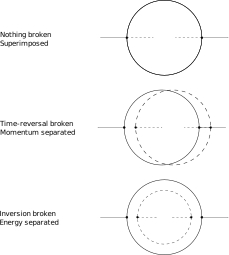
\includegraphics[width=0.75\textwidth]{figures/spinStructureWeyl}
  \caption{\label{fig:spinStructure} }
\end{figure}

\section{Only translationally invariant systems have conservation of momentum in correlators}
\todo{rewrite section title}
\begin{theorem}
  If the momentum space correlator is $\braket{A(p)B(-p)}$, the real space correlator is translationally invariant.
\end{theorem}
\begin{Proof}
Consider the correlator
\begin{equation}
  \Braket{A(x)B(y)}.
\end{equation}
If its momentum space equivalent is
\begin{equation}
  \Braket{A(q)B(-q)} = \Braket{A(q)B(p)} \delta (p+q),
\end{equation}
then the real space correlator is given by
\begin{equation}
  \int \mathrm{d}p \mathrm{d}q
  \Braket{A(p)B(q)}\delta (p+q)
  e^{ipx + iqy}
  = \int \mathrm{d}p \Braket{A(p)B(-p)} e^{ip(x-y)}.
\end{equation}
This function is only dependent on $x-y$, and thus translationally invariant.
Therefore, the only way to get a correlator on the form $\braket{A(p)B(-p)}$ is to assume trnaslational invariance.
\end{Proof}

\section{Removing the explicit tilt from the Lagrangian by a non-flat metric}\label{sec:tilt-metric}
In the main text, we have used the Lagrangian
\begin{equation}
  L_s = i \phi^{\dagger} \tilde{\sigma} ^{\mu} \partial_{\mu} \phi,
\end{equation}
where we defined the \emph{modified} Pauli matrices \( \tilde{\sigma} ^{\mu}= \sigma^{\mu} + t^{\mu}, \; t^{\mu} = (0, \vec{t}) \).
We here present an alternative, where we instead consider moving the tilting into the metric, i.e. considering a non-tilted cone in curved spacetime.
In essence, we want
\[
g^{\mu \nu} \sigma_{\nu} p_{\mu}
\]
to give \( (\sigma^{\mu} + t^{\mu}) p_{\mu} \).
We see that this involves putting \( t^{\mu} \) on the 0-components of the metric.

Consider the metric
\begin{equation}
  g^{\mu \nu} = \eta^{\mu \nu } + t^{\mu} (\delta^{\mu}_0 + \delta^{\nu}_0) =
  \begin{pmatrix}
    1 & t^x & t^y & t^z\\
    t^x & -1 & 0 &0\\
    t^y & 0 & -1 &0\\
    t^z & 0 & 0 &-1
  \end{pmatrix}.
\end{equation}
The top row is however problematic, as it gives an unwanted
\[
g^{0 \nu} \sigma_{\nu} = \sigma^0 - \vec{t} \vec{\sigma}.
\]
Interestingly, the metric thus \emph{cannot} be symmetric!
We conclude that the appropriate choice is
\begin{equation}
  g^{\mu \nu} = \eta^{\mu \nu } + t^{\mu} \delta^{\nu}_0 =
  \begin{pmatrix}
    1 & 0 & 0 & 0\\
    t^x & -1 & 0 &0\\
    t^y & 0 & -1 &0\\
    t^z & 0 & 0 &-1
  \end{pmatrix}.
\end{equation}

Consider therefore the Lagrangian
\begin{equation}
  \mathcal{L} = \phi^{\dagger} g^{\mu \sigma} \sigma_{\sigma} \partial_{\mu} \phi.
\end{equation}
Using once again the canoncial defintion
\begin{align}
  T^{\mu \nu} &= \frac{\partial \mathcal{L}}{\partial(\partial_{\mu}\phi)} \partial^{\nu} \phi\\
  &= \phi^{\dagger} g^{\mu \sigma} \sigma_{\sigma} \partial^{\nu} \phi,
\end{align}
we find the component of the energy-momentum tensor
\begin{equation}
  T^{y 0} = \phi^{\dagger} g^{y \sigma} \sigma_{\sigma} \partial^0 \phi =
  \phi^{\dagger} (t^y \sigma_0 + \sigma_y) \partial^0 \phi.
\end{equation}

\begin{remark}
  The four-Pauli matrices are defined as
  \begin{equation}
    \sigma^{\mu} = (\sigma^0, \sigma^1, \sigma^2, \sigma^{3}) = (\sigma^0, \sigma_x, \sigma_y, \sigma_z),
  \end{equation}
  where the matrices with lower roman indices are the well-known Pauli matrices.
  Thus, the four-matrices with lowered inddex are
  \begin{equation}
    \sigma_{\mu} = \eta_{\mu \nu} \sigma^{\mu} = (\sigma^0, -\sigma^1, -\sigma^2, -\sigma^{3}).
  \end{equation}
\end{remark}


\backmatter
\nocite{Mathematica}
\printbibliography[heading=bibintoc]

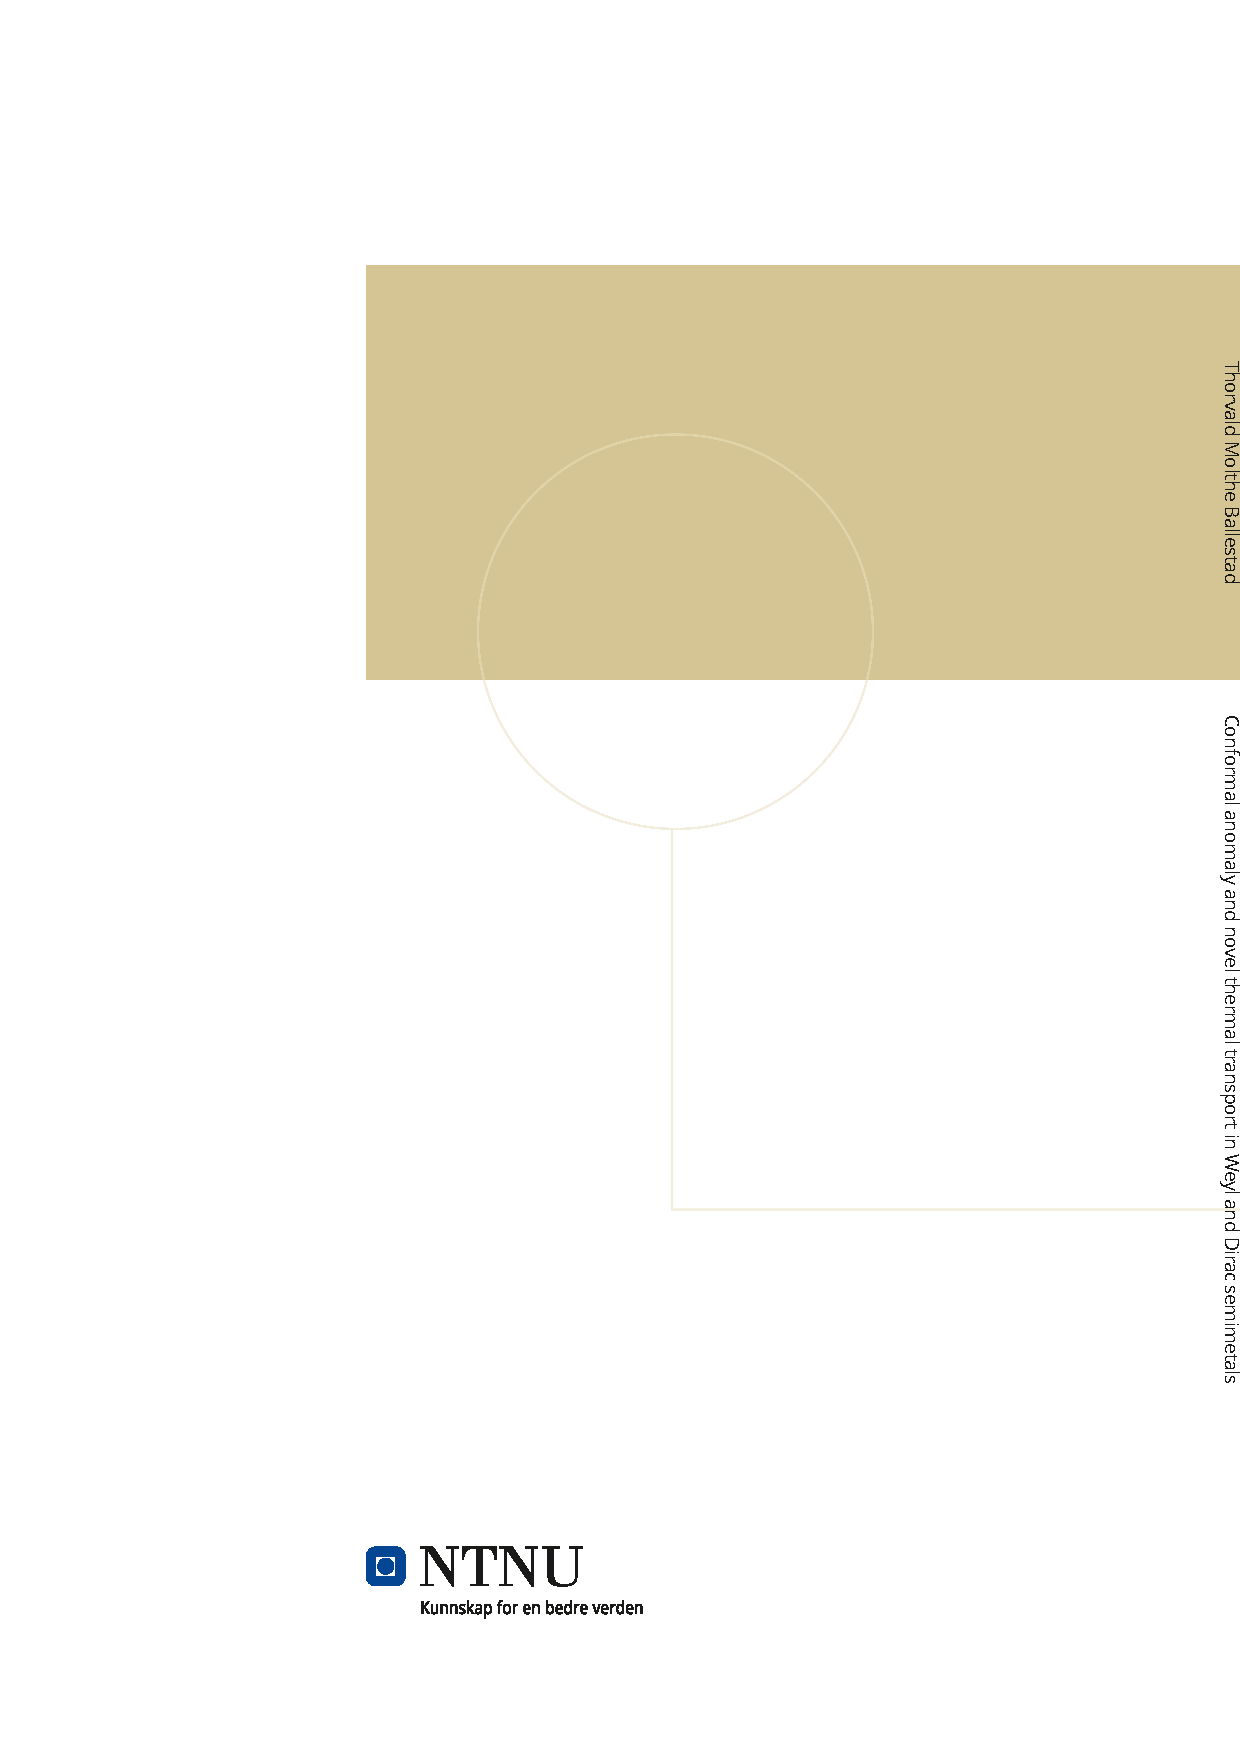
\includepdf{endpagethesis.pdf}
\end{document}
